% -*- Mode:TeX -*-

%% IMPORTANT: The official thesis specifications are available at:
%%            http://libraries.mit.edu/archives/thesis-specs/
%%
%%            Please verify your thesis' formatting and copyright
%%            assignment before submission.  If you notice any
%%            discrepancies between these templates and the 
%%            MIT Libraries' specs, please let us know
%%            by e-mailing thesis@mit.edu

%% The documentclass options along with the pagestyle can be used to generate
%% a technical report, a draft copy, or a regular thesis.  You may need to
%% re-specify the pagestyle after you \include  cover.tex.  For more
%% information, see the first few lines of mitthesis.cls. 

%\documentclass[12pt,vi,twoside]{mitthesis}
%%
%%  If you want your thesis copyright to you instead of MIT, use the
%%  ``vi'' option, as above.
%%
%\documentclass[12pt,twoside,leftblank]{mitthesis}
%%
%% If you want blank pages before new chapters to be labelled ``This
%% Page Intentionally Left Blank'', use the ``leftblank'' option, as
%% above. 

\documentclass[12pt,twoside]{mitthesis}
\usepackage{lgrind}
%% These have been added at the request of the MIT Libraries, because
%% some PDF conversions mess up the ligatures.  -LB, 1/22/2014
\usepackage{cmap}
\usepackage[T1]{fontenc}
\usepackage{graphicx}
\usepackage{multirow}
\usepackage{url}
%\usepackage[numbers,sort]{natbib}
\pagestyle{plain}
\usepackage{amsmath}

%% This bit allows you to either specify only the files which you wish to
%% process, or `all' to process all files which you \include.
%% Krishna Sethuraman (1990).

\typein [\files]{Enter file names to process, (chap1,chap2 ...), or `all' to
process all files:}
\def\all{all}
\ifx\files\all \typeout{Including all files.} \else \typeout{Including only \files.} \includeonly{\files} \fi

\begin{document}
\newcommand{\CLs}{\ensuremath{CL_\mathrm{s}}}
\newcommand{\CLb}{\ensuremath{CL_\mathrm{b}}}
\newcommand{\CLsb}{\ensuremath{CL_\mathrm{s+b}}}

\newcommand{\GeV}{\ensuremath{\mathrm{Ge\kern -0.1em V}}}
\newcommand{\TeV}{\ensuremath{\mathrm{Te\kern -0.1em V}}}
\newcommand{\TeVcc}{\ensuremath{\,\mathrm{Te\kern -0.1em V\!/c}^2}}
\newcommand{\GeVcc}{\ensuremath{\,\mathrm{Ge\kern -0.1em V\!/c}^2}}
\newcommand{\MeVcc}{\ensuremath{\,\mathrm{Me\kern -0.1em V\!/c}^2}}
\newcommand{\GeVc}{\ensuremath{\mathrm{Ge\kern -0.1em V}\!/c}}
\newcommand{\nanob}{\mbox{{\rm ~nb}~}}
\newcommand{\fb}{\ensuremath{\mathrm{fb}}}
\newcommand{\pb}{\ensuremath{\mathrm{pb}}}
\newcommand{\ifb}{\ensuremath{\mathrm{fb^{-1}}}}
\newcommand{\ipb}{\ensuremath{\mathrm{pb^{-1}}}}
\newcommand{\grad}{\ensuremath{^{\circ}}}

%
% Special user made math symbols
%
%\newcommand{\lsim}{\raisebox{-1.5mm}{$\:\stackrel{\textstyle{<}}{\textstyle{\sim}}\:$}}
%\newcommand{\gsim}{\raisebox{-1.5mm}{$\:\stackrel{\textstyle{>}}{\textstyle{\sim}}\:$}}

% particles
\newcommand{\pipm}{\ensuremath{\pi^{\pm}}}
\newcommand{\pizero}{\ensuremath{\pi^{0}}}
\newcommand{\Hi}{\PH\xspace}
\newcommand{\V}{\ensuremath{\mathrm{V}}}
\newcommand{\W}{\PW}
\newcommand{\Wjets}{\ensuremath{\mathrm{W+jets}}}
\newcommand{\Zjets}{\ensuremath{\mathrm{Z+jets}}}
\newcommand{\Wt}{\ensuremath{\mathrm{Wt}}}
\newcommand{\Wstar}{\ensuremath{\mathrm{W}^{*}}}
\newcommand{\Wparenthesisstar}{\ensuremath{\mathrm{W}^{(*)}}}
\newcommand{\WW}{\PW\PW\xspace}
\newcommand{\Z}{\ensuremath{\mathrm{Z}}}
\newcommand{\Zstar}{\ensuremath{\mathrm{Z}^{*}}}
\newcommand{\Astar}{\ensuremath{\mathrm{\gamma}^{*}}}
\newcommand{\ZZ}{\ensuremath{\Z\Z}}
\newcommand{\WZ}{\ensuremath{\W\Z}}
\newcommand{\VVV}{\ensuremath{\V\V\V}}
\newcommand{\Wgstar}{\ensuremath{\W\gamma}^{*}}
\newcommand{\E}{\Pe}
\newcommand{\Ep}{\Pep}
\newcommand{\Em}{\ensuremath{\mathrm{e}^{-}}}
\newcommand{\Epm}{\ensuremath{\Pe^{\pm}}}
\newcommand{\Emp}{\ensuremath{\Pe^{\mp}}}
\newcommand{\M}{\Pgm}
\newcommand{\Mp}{\Pgmp}
\newcommand{\Mm}{\Pgmm}
\newcommand{\Mpm}{\ensuremath{\mu^{\pm}}}
\newcommand{\Mmp}{\ensuremath{\mu^{\mp}}}
\newcommand{\Tau}{\ensuremath{\tau}}
\newcommand{\Nu}{\ensuremath{\nu}}
\newcommand{\Nubar}{\ensuremath{\overline{\nu}}}
\newcommand{\Lep}{\ensuremath{\ell}}
\newcommand{\Lepp}{\ensuremath{\ell^{+}}}
\newcommand{\Lepm}{\ensuremath{\ell^{-}}}
\newcommand{\Lprime}{\ensuremath{\Lep^{\prime}}}
\newcommand{\Prot}{\Pp}
\newcommand{\Pbar}{\Pap}
\newcommand{\PP}{\Pp\Pp}
\newcommand{\PPbar}{\Pp\Pap}
\newcommand{\ttbar}{\ensuremath{\mathrm{t}\bar{\mathrm{t}}}}
\newcommand{\qq}{\ensuremath{\mathrm{q}\mathrm{q}}}
\newcommand{\qqbar}{\ensuremath{\mathrm{q}\overline{\mathrm{q}}}}
\newcommand{\Wtb}{\ensuremath{\W\mathrm{t}\mathrm{b}}}
\newcommand{\Top}{\ensuremath{\mathrm{t}}}
\newcommand{\Bot}{\ensuremath{\mathrm{b}}}
\newcommand{\Atop}{\ensuremath{\overline{\mathrm{t}}}}
\newcommand{\Abot}{\ensuremath{\overline{\mathrm{b}}}}
% arrow
\newcommand{\To}{\ensuremath{\rightarrow}}

% masses
\newcommand{\mH}{\ensuremath{m_{\PH}}}
\newcommand{\mHi}{\ensuremath{m_{\PH}}\xspace}
\newcommand{\mW}{\ensuremath{m_{\PW}}}
\newcommand{\mZ}{\ensuremath{m_{\cPZ}}}
\newcommand{\mll}{\ensuremath{m_{\Lep\Lep}}}
\newcommand{\mt}{\ensuremath{m_{\mathrm{T}}}}
%%%\newcommand{\mth}{\ensuremath{m_{\mathrm{T}}^{\ell\ell\not{E}_{\mathrm T}}}}
\newcommand{\mth}{\ensuremath{m_{\mathrm{T}}}}
\newcommand{\mtlnjj}{\ensuremath{m_{\mathrm{T}}^{\ell\nu 2j}}}
\newcommand{\mr}{\ensuremath{m_{\mathrm{R}}}}
\newcommand{\delphir}{\ensuremath{\Delta\phi_{\mathrm{R}}}}

% generators
\newcommand{\pythia} {\textsc{pythia}}
\newcommand{\geant} {\textsc{geant4}}
\newcommand{\herwig} {\textsc{herwig}}
\newcommand{\acermc} {\textsc{acermc}}
\newcommand{\jimmy} {\textsc{jimmy}}
\newcommand{\mcatnlo} {\textsc{mc@nlo}}
\newcommand{\sherpa} {\textsc{sherpa}}
\newcommand{\madgraph} {\textsc{madgraph}}
\newcommand{\mcfm} {\textsc{mcfm}}
\newcommand{\powheg} {\textsc{powheg}}
\newcommand{\Phantom} {\textsc{phantom}}
\newcommand{\fastjet} {\textsc{fastJet}}
\newcommand{\tauola} {\textsc{tauola}}

% kinematics
% \newcommand{\pt}{\ensuremath{p_\mathrm{T}}}
\newcommand{\Et}{\ensuremath{E_\mathrm{T}}}
\newcommand{\ptveto}{\ensuremath{\pt^\text{veto}}}
\newcommand{\ptl}{\ensuremath{p_\perp^{\Lep}}}
\newcommand{\ptlmax}{\ensuremath{p_{\mathrm{T}}^{\Lep,\text{max}}}}
\newcommand{\ptlmin}{\ensuremath{p_{\mathrm{T}}^{\Lep,\text{min}}}}
\newcommand{\ptll}{\ensuremath{\pt^{\ell\ell}}}
\newcommand{\met}{\ensuremath{\Et^{\text{miss}}}}
\newcommand{\delphill}{\ensuremath{\Delta\phi_{\Lep\Lep}}}
\newcommand{\deletall}{\ensuremath{\Delta\eta_{\Lep\Lep}}}
\newcommand{\delphimetl}{\ensuremath{\Delta\phi(\vec{E}_\mathrm{T}^{\text{miss}},\Lep)}}
\newcommand{\delphillmet}{\ensuremath{\Delta\phi(\Lep\Lep,\vec{E}_\mathrm{T}^{\text{miss}})}}
\newcommand{\delR}{\ensuremath{\Delta R}}
\newcommand{\Eta}{\ensuremath{\eta}}
\newcommand{\GAMMA}{\ensuremath{\gamma}}
\newcommand{\pmet}{\ensuremath{E^{\text{miss}\angle}_\mathrm{T}}}
\newcommand{\vmet}{\ensuremath{\vec{E}_\mathrm{T}}^{\text{miss}}}

%efficiencies
\newcommand{\effsig}{\ensuremath{\varepsilon_{\text{bkg}}^{\mathrm{S}}}}
\newcommand{\effnorm}{\ensuremath{\varepsilon_{\text{bkg}}^{\mathrm{N}}}}
\newcommand{\Nsig}{\ensuremath{N_{\text{bkg}}^{\mathrm{S}}}}
\newcommand{\Nnorm}{\ensuremath{N_{\text{bkg}}^{\mathrm{N}}}}

% processes
\newcommand{\dyeepm}{\ensuremath{{\Z}/\GAMMA^*{\to \Pep\Pem}}}
\newcommand{\dymmpm}{\ensuremath{{\Z/}\GAMMA^*\to\Pgmp\Pgmm}}
\newcommand{\dyttpm}{\ensuremath{{\Z}/\GAMMA^* \to\tau^+\tau^-}}
\newcommand{\dyllpm}{\ensuremath{{\Z}/\GAMMA^*{\to \ell^+\ell^-}}}
\newcommand{\dyee}{\ensuremath{{\Z}/\GAMMA^*{\to \Pe\Pe}}}
\newcommand{\dymm}{\ensuremath{{\Z/}\GAMMA^*\to\mu\mu}}
\newcommand{\dytt}{\ensuremath{{\Z}/\GAMMA^* \to\tau\tau}}
\newcommand{\dyll}{\ensuremath{{\Z}/\GAMMA^*{\to \ell\ell}}}
\newcommand{\zee}{\ensuremath{{\Z\to \Pep\Pem}}}
\newcommand{\zmm}{\ensuremath{{\Z}\to\Pgmp\Pgmm}}
\newcommand{\ztt}{\ensuremath{{\Z}\to\tau^+\tau^-}}
\newcommand{\zll}{\ensuremath{{\Z\to \ell^+\ell^-}}}
\newcommand{\ppww}{\ensuremath{pp \to \PWp\PWm}}
\newcommand{\wwlnln}{\ensuremath{\PWp\PWm\to \ell^+\nu \ell^-\overline{\nu}}}
\newcommand{\ww}{\ensuremath{\W\W}}
\newcommand{\WWpm}{\ensuremath{\PWp\PWm}}
\newcommand{\Hww}{\Hi\to\WW}
\newcommand{\hww}{\Hi\to\WW}
\newcommand{\hwwnopm}{\Hi\to\ww}
\newcommand{\hwwlnlnnopm}{\ensuremath{\Hi\to \W\W\to \ell \nu \ell \nu}}
\newcommand{\wz}{{\PW\cPZ}}
\newcommand{\zz}{{\cPZ\cPZ}}
\newcommand{\wgamma}{\ensuremath{\W\GAMMA}}
\newcommand{\wjets}{\ensuremath{\PW+}\text{jets}}
\newcommand{\tw}{\ensuremath{\mathrm{t}\W}}
\newcommand{\singletopt}{\ensuremath{t} ($t$-chan)}
\newcommand{\singletops}{\ensuremath{t} ($s$-chan)}

%other
\def\fixme{({\bf FixMe})}
\newcommand{\ee}{\ensuremath{ee}}
\newcommand{\emu}{\ensuremath{e\mu}}
\def\mm{\ensuremath{\mu\mu}}
\newcommand{\spintwopmin}{\ensuremath{2^+_\text{min}}}

% integrated luminosity
\newcommand{\usedLumi}{19.7 \fbinv}
\newcommand{\usedLumiWithSyst}{\ensuremath{19.7 \pm 0.5 \fbinv}}


% -*-latex-*-
% 
% For questions, comments, concerns or complaints:
% thesis@mit.edu
% 
%
% $Log: cover.tex,v $
% Revision 1.8  2008/05/13 15:02:15  jdreed
% Degree month is June, not May.  Added note about prevdegrees.
% Arthur Smith's title updated
%
% Revision 1.7  2001/02/08 18:53:16  boojum
% changed some \newpages to \cleardoublepages
%
% Revision 1.6  1999/10/21 14:49:31  boojum
% changed comment referring to documentstyle
%
% Revision 1.5  1999/10/21 14:39:04  boojum
% *** empty log message ***
%
% Revision 1.4  1997/04/18  17:54:10  othomas
% added page numbers on abstract and cover, and made 1 abstract
% page the default rather than 2.  (anne hunter tells me this
% is the new institute standard.)
%
% Revision 1.4  1997/04/18  17:54:10  othomas
% added page numbers on abstract and cover, and made 1 abstract
% page the default rather than 2.  (anne hunter tells me this
% is the new institute standard.)
%
% Revision 1.3  93/05/17  17:06:29  starflt
% Added acknowledgements section (suggested by tompalka)
% 
% Revision 1.2  92/04/22  13:13:13  epeisach
% Fixes for 1991 course 6 requirements
% Phrase "and to grant others the right to do so" has been added to 
% permission clause
% Second copy of abstract is not counted as separate pages so numbering works
% out
% 
% Revision 1.1  92/04/22  13:08:20  epeisach

% NOTE:
% These templates make an effort to conform to the MIT Thesis specifications,
% however the specifications can change.  We recommend that you verify the
% layout of your title page with your thesis advisor and/or the MIT 
% Libraries before printing your final copy.
\title{Electroweak physics and evidence for a Higgs Boson in leptonic decays with the CMS Detector}

\author{Aram Apyan}
% If you wish to list your previous degrees on the cover page, use the 
% previous degrees command:
%       \prevdegrees{A.A., Harvard University (1985)}
% You can use the \\ command to list multiple previous degrees
%       \prevdegrees{B.S., University of California (1978) \\
%                    S.M., Massachusetts Institute of Technology (1981)}
\department{Department of Physics}

% If the thesis is for two degrees simultaneously, list them both
% separated by \and like this:
% \degree{Doctor of Philosophy \and Master of Science}
\degree{Doctor of Philosophy in Physics}

% As of the 2007-08 academic year, valid degree months are September, 
% February, or June.  The default is June.
\degreemonth{September}
\degreeyear{2016}
\thesisdate{September 30, 2016}

%% By default, the thesis will be copyrighted to MIT.  If you need to copyright
%% the thesis to yourself, just specify the `vi' documentclass option.  If for
%% some reason you want to exactly specify the copyright notice text, you can
%% use the \copyrightnoticetext command.  
%\copyrightnoticetext{\copyright IBM, 1990.  Do not open till Xmas.}

% If there is more than one supervisor, use the \supervisor command
% once for each.
\supervisor{Markus Klute}{Associate Professor}

% This is the department committee chairman, not the thesis committee
% chairman.  You should replace this with your Department's Committee
% Chairman.
\chairman{Professor Nergis Mavalvala}{Associate Department Head for Education}

% Make the titlepage based on the above information.  If you need
% something special and can't use the standard form, you can specify
% the exact text of the titlepage yourself.  Put it in a titlepage
% environment and leave blank lines where you want vertical space.
% The spaces will be adjusted to fill the entire page.  The dotted
% lines for the signatures are made with the \signature command.
\maketitle

% The abstractpage environment sets up everything on the page except
% the text itself.  The title and other header material are put at the
% top of the page, and the supervisors are listed at the bottom.  A
% new page is begun both before and after.  Of course, an abstract may
% be more than one page itself.  If you need more control over the
% format of the page, you can use the abstract environment, which puts
% the word "Abstract" at the beginning and single spaces its text.

%% You can either \input (*not* \include) your abstract file, or you can put
%% the text of the abstract directly between the \begin{abstractpage} and
%% \end{abstractpage} commands.

% First copy: start a new page, and save the page number.
\cleardoublepage
% Uncomment the next line if you do NOT want a page number on your
% abstract and acknowledgments pages.
% \pagestyle{empty}
\setcounter{savepage}{\thepage}
\begin{abstractpage}
% $Log: abstract.tex,v $
% Revision 1.1  93/05/14  14:56:25  starflt
% Initial revision
% 
% Revision 1.1  90/05/04  10:41:01  lwvanels
% Initial revision
% 
%
%% The text of your abstract and nothing else (other than comments) goes here.
%% It will be single-spaced and the rest of the text that is supposed to go on
%% the abstract page will be generated by the abstractpage environment.  This
%% file should be \input (not \include 'd) from cover.tex.
Hey hey hey ...
\end{abstractpage}

% Additional copy: start a new page, and reset the page number.  This way,
% the second copy of the abstract is not counted as separate pages.
% Uncomment the next 6 lines if you need two copies of the abstract
% page.
% \setcounter{page}{\thesavepage}
% \begin{abstractpage}
% % $Log: abstract.tex,v $
% Revision 1.1  93/05/14  14:56:25  starflt
% Initial revision
% 
% Revision 1.1  90/05/04  10:41:01  lwvanels
% Initial revision
% 
%
%% The text of your abstract and nothing else (other than comments) goes here.
%% It will be single-spaced and the rest of the text that is supposed to go on
%% the abstract page will be generated by the abstractpage environment.  This
%% file should be \input (not \include 'd) from cover.tex.
Hey hey hey ...
% \end{abstractpage}

\cleardoublepage

\section*{Acknowledgments}

I would like to express my deep gratitude to La Meyrinoise for providing excellent Tiramisu throughout last four years.      

%%%%%%%%%%%%%%%%%%%%%%%%%%%%%%%%%%%%%%%%%%%%%%%%%%%%%%%%%%%%%%%%%%%%%%
% -*-latex-*-

% Some departments (e.g. 5) require an additional signature page.  See
% signature.tex for more information and uncomment the following line if
% applicable.
% % -*- Mode:TeX -*-
%
% Some departments (e.g. Chemistry) require an additional cover page
% with signatures of the thesis committee.  Please check with your
% thesis advisor or other appropriate person to determine if such a 
% page is required for your thesis.  
%
% If you choose not to use the "titlepage" environment, a \newpage
% commands, and several \vspace{\fill} commands may be necessary to
% achieve the required spacing.  The \signature command is defined in
% the "mitthesis" class
%
% The following sample appears courtesy of Ben Kaduk <kaduk@mit.edu> and
% was used in his June 2012 doctoral thesis in Chemistry. 

\begin{titlepage}
\begin{large}
This doctoral thesis has been examined by a Committee of the Department
of Chemistry as follows:

\signature{Professor Jianshu Cao}{Chairman, Thesis Committee \\
   Professor of Chemistry}

\signature{Professor Troy Van Voorhis}{Thesis Supervisor \\
   Associate Professor of Chemistry}

\signature{Professor Robert W. Field}{Member, Thesis Committee \\
   Haslam and Dewey Professor of Chemistry}
\end{large}
\end{titlepage}


\pagestyle{plain}
  % -*- Mode:TeX -*-
%% This file simply contains the commands that actually generate the table of
%% contents and lists of figures and tables.  You can omit any or all of
%% these files by simply taking out the appropriate command.  For more
%% information on these files, see appendix C.3.3 of the LaTeX manual. 
\tableofcontents
\newpage
\listoffigures
\newpage
\listoftables


%%% This is an example first chapter.  You should put chapter/appendix that you
%% write into a separate file, and add a line \include{yourfilename} to
%% main.tex, where `yourfilename.tex' is the name of the chapter/appendix file.
%% You can process specific files by typing their names in at the 
%% \files=
%% prompt when you run the file main.tex through LaTeX.
\chapter{Introduction}

Micro-optimization is a technique to reduce the overall operation count of
floating point operations.  In a standard floating point unit, floating
point operations are fairly high level, such as ``multiply'' and ``add'';
in a micro floating point unit ($\mu$FPU), these have been broken down into
their constituent low-level floating point operations on the mantissas and
exponents of the floating point numbers.

Chapter two describes the architecture of the $\mu$FPU unit, and the
motivations for the design decisions made.

Chapter three describes the design of the compiler, as well as how the
optimizations discussed in section~\ref{ch1:opts} were implemented.

Chapter four describes the purpose of test code that was compiled, and which
statistics were gathered by running it through the simulator.  The purpose
is to measure what effect the micro-optimizations had, compared to
unoptimized code.  Possible future expansions to the project are also
discussed.

\section{Motivations for micro-optimization}

The idea of micro-optimization is motivated by the recent trends in computer
architecture towards low-level parallelism and small, pipelineable
instruction sets \cite{patterson:risc,rad83}.  By getting rid of more
complex instructions and concentrating on optimizing frequently used
instructions, substantial increases in performance were realized.

Another important motivation was the trend towards placing more of the
burden of performance on the compiler.  Many of the new architectures depend
on an intelligent, optimizing compiler in order to realize anywhere near
their peak performance
\cite{ellis:bulldog,pet87,coutant:precision-compilers}.  In these cases, the
compiler not only is responsible for faithfully generating native code to
match the source language, but also must be aware of instruction latencies,
delayed branches, pipeline stages, and a multitude of other factors in order
to generate fast code \cite{gib86}.

Taking these ideas one step further, it seems that the floating point
operations that are normally single, large instructions can be further broken
down into smaller, simpler, faster instructions, with more control in the
compiler and less in the hardware.  This is the idea behind a
micro-optimizing FPU; break the floating point instructions down into their
basic components and use a small, fast implementation, with a large part of
the burden of hardware allocation and optimization shifted towards
compile-time.

Along with the hardware speedups possible by using a $\mu$FPU, there are
also optimizations that the compiler can perform on the code that is
generated.  In a normal sequence of floating point operations, there are
many hidden redundancies that can be eliminated by allowing the compiler to
control the floating point operations down to their lowest level.  These
optimizations are described in detail in section~\ref{ch1:opts}.

\section{Description of micro-optimization}\label{ch1:opts}

In order to perform a sequence of floating point operations, a normal FPU
performs many redundant internal shifts and normalizations in the process of
performing a sequence of operations.  However, if a compiler can
decompose the floating point operations it needs down to the lowest level,
it then can optimize away many of these redundant operations.  

If there is some additional hardware support specifically for
micro-optimization, there are additional optimizations that can be
performed.  This hardware support entails extra ``guard bits'' on the
standard floating point formats, to allow several unnormalized operations to
be performed in a row without the loss information\footnote{A description of
the floating point format used is shown in figures~\ref{exponent-format}
and~\ref{mantissa-format}.}.  A discussion of the mathematics behind
unnormalized arithmetic is in appendix~\ref{unnorm-math}.

The optimizations that the compiler can perform fall into several categories:

\subsection{Post Multiply Normalization}

When more than two multiplications are performed in a row, the intermediate
normalization of the results between multiplications can be eliminated.
This is because with each multiplication, the mantissa can become
denormalized by at most one bit.  If there are guard bits on the mantissas
to prevent bits from ``falling off'' the end during multiplications, the
normalization can be postponed until after a sequence of several
multiplies\footnote{Using unnormalized numbers for math is not a new idea; a
good example of it is the Control Data CDC 6600, designed by Seymour Cray.
\cite{thornton:cdc6600} The CDC 6600 had all of its instructions performing
unnormalized arithmetic, with a separate {\tt NORMALIZE} instruction.}.

% This is an example of how you would use tgrind to include an example
% of source code; it is commented out in this template since the code
% example file does not exist.  To use it, you need to remove the '%' on the
% beginning of the line, and insert your own information in the call.
%
%\tagrind[htbp]{code/pmn.s.tex}{Post Multiply Normalization}{opt:pmn}

As you can see, the intermediate results can be multiplied together, with no
need for intermediate normalizations due to the guard bit.  It is only at
the end of the operation that the normalization must be performed, in order
to get it into a format suitable for storing in memory\footnote{Note that
for purposed of clarity, the pipeline delays were considered to be 0, and
the branches were not delayed.}.

\subsection{Block Exponent}

In a unoptimized sequence of additions, the sequence of operations is as
follows for each pair of numbers ($m_1$,$e_1$) and ($m_2$,$e_2$).
\begin{enumerate}
  \item Compare $e_1$ and $e_2$.
  \item Shift the mantissa associated with the smaller exponent $|e_1-e_2|$
        places to the right.
  \item Add $m_1$ and $m_2$.
  \item Find the first one in the resulting mantissa.
  \item Shift the resulting mantissa so that normalized
  \item Adjust the exponent accordingly.
\end{enumerate}

Out of 6 steps, only one is the actual addition, and the rest are involved
in aligning the mantissas prior to the add, and then normalizing the result
afterward.  In the block exponent optimization, the largest mantissa is
found to start with, and all the mantissa's shifted before any additions
take place.  Once the mantissas have been shifted, the additions can take
place one after another\footnote{This requires that for n consecutive
additions, there are $\log_{2}n$ high guard bits to prevent overflow.  In
the $\mu$FPU, there are 3 guard bits, making up to 8 consecutive additions
possible.}.  An example of the Block Exponent optimization on the expression
X = A + B + C is given in figure~\ref{opt:be}.

% This is an example of how you would use tgrind to include an example
% of source code; it is commented out in this template since the code
% example file does not exist.  To use it, you need to remove the '%' on the
% beginning of the line, and insert your own information in the call.
%
%\tgrind[htbp]{code/be.s.tex}{Block Exponent}{opt:be}

\section{Integer optimizations}

As well as the floating point optimizations described above, there are
also integer optimizations that can be used in the $\mu$FPU.  In concert
with the floating point optimizations, these can provide a significant
speedup.  

\subsection{Conversion to fixed point}

Integer operations are much faster than floating point operations; if it is
possible to replace floating point operations with fixed point operations,
this would provide a significant increase in speed.

This conversion can either take place automatically or or based on a
specific request from the programmer.  To do this automatically, the
compiler must either be very smart, or play fast and loose with the accuracy
and precision of the programmer's variables.  To be ``smart'', the computer
must track the ranges of all the floating point variables through the
program, and then see if there are any potential candidates for conversion
to floating point.  This technique is discussed further in
section~\ref{range-tracking}, where it was implemented.

The other way to do this is to rely on specific hints from the programmer
that a certain value will only assume a specific range, and that only a
specific precision is desired.  This is somewhat more taxing on the
programmer, in that he has to know the ranges that his values will take at
declaration time (something normally abstracted away), but it does provide
the opportunity for fine-tuning already working code.

Potential applications of this would be simulation programs, where the
variable represents some physical quantity; the constraints of the physical
system may provide bounds on the range the variable can take.
\subsection{Small Constant Multiplications}

One other class of optimizations that can be done is to replace
multiplications by small integer constants into some combination of
additions and shifts.  Addition and shifting can be significantly faster
than multiplication.  This is done by using some combination of
\begin{eqnarray*}
a_i & = & a_j + a_k \\
a_i & = & 2a_j + a_k \\
a_i & = & 4a_j + a_k \\
a_i & = & 8a_j + a_k \\
a_i & = & a_j - a_k \\
a_i & = & a_j \ll m \mbox{shift}
\end{eqnarray*}
instead of the multiplication.  For example, to multiply $s$ by 10 and store
the result in $r$, you could use:
\begin{eqnarray*}
r & = & 4s + s\\
r & = & r + r
\end{eqnarray*}
Or by 59:
\begin{eqnarray*}
t & = & 2s + s \\
r & = & 2t + s \\
r & = & 8r + t
\end{eqnarray*}
Similar combinations can be found for almost all of the smaller
integers\footnote{This optimization is only an ``optimization'', of course,
when the amount of time spent on the shifts and adds is less than the time
that would be spent doing the multiplication.  Since the time costs of these
operations are known to the compiler in order for it to do scheduling, it is
easy for the compiler to determine when this optimization is worth using.}.
\cite{magenheimer:precision}

\section{Other optimizations}

\subsection{Low-level parallelism}

The current trend is towards duplicating hardware at the lowest level to
provide parallelism\footnote{This can been seen in the i860; floating point
additions and multiplications can proceed at the same time, and the RISC
core be moving data in and out of the floating point registers and providing
flow control at the same time the floating point units are active. \cite{byte:i860}}

Conceptually, it is easy to take advantage to low-level parallelism in the
instruction stream by simply adding more functional units to the $\mu$FPU,
widening the instruction word to control them, and then scheduling as many
operations to take place at one time as possible.

However, simply adding more functional units can only be done so many times;
there is only a limited amount of parallelism directly available in the
instruction stream, and without it, much of the extra resources will go to
waste.  One process used to make more instructions potentially schedulable
at any given time is ``trace scheduling''.  This technique originated in the
Bulldog compiler for the original VLIW machine, the ELI-512.
\cite{ellis:bulldog,colwell:vliw}  In trace scheduling, code can be
scheduled through many basic blocks at one time, following a single
potential ``trace'' of program execution.  In this way, instructions that
{\em might\/} be executed depending on a conditional branch further down in
the instruction stream are scheduled, allowing an increase in the potential
parallelism.  To account for the cases where the expected branch wasn't
taken, correction code is inserted after the branches to undo the effects of
any prematurely executed instructions.

\subsection{Pipeline optimizations}

In addition to having operations going on in parallel across functional
units, it is also typical to have several operations in various stages of
completion in each unit.  This pipelining allows the throughput of the
functional units to be increased, with no increase in latency.

There are several ways pipelined operations can be optimized.  On the
hardware side, support can be added to allow data to be recirculated back
into the beginning of the pipeline from the end, saving a trip through the
registers.  On the software side, the compiler can utilize several tricks to
try to fill up as many of the pipeline delay slots as possible, as
seendescribed by Gibbons. \cite{gib86}



%% This is an example first chapter.  You should put chapter/appendix that you
%% write into a separate file, and add a line \include{yourfilename} to
%% main.tex, where `yourfilename.tex' is the name of the chapter/appendix file.
%% You can process specific files by typing their names in at the 
%% \files=
%% prompt when you run the file main.tex through LaTeX.

\chapter{Introduction}

The Standard Model (SM) theory of elementary particles provides a remarkably successful description of many experimental results up to currently accessible energies. Leptons and colored quarks are the building blocks of matter and the SM provides a fundamental theory of strong~\cite{Politzer:1973fx,Gross:1973id} and electroweak interactions~\cite{Glashow:1961tr,Weinberg:1967tq,Salam:1968rm}. The strong interactions are mediated by massless gluons, and the force carriers of the electroweak interactions are the massless photon and the massive $W$ and $Z$ bosons. The SM is a renormalizable gauge theory based on the symmetry group $SU(3) \times SU(2) \times U(1)$. However the massive $W$ and $Z$ gauge bosons and the massless photon clearly brake the electroweak symmetry. It was shown that the masses can be generated through spontaneous symmetry breaking by adding a complex scalar field to the model~\cite{Englert:1964et,Higgs:1964ia,Higgs:1964pj,Guralnik:1964eu,Higgs:1966ev,Kibble:1967sv}. A physical neutral heavy scalar boson, the SM Higgs boson ($H$), remains after the spontaneous symmetry breaking for a complex scalar Higgs doublet. The scalar field can also account for the fundamental fermion masses. Postulated Yukawa couplings of the Higgs field to the fundamental fermions introduces the fermion mass terms after the same spontaneous symmetry breaking mechanism that gives masses to the $W$ and $Z$ gauge bosons. 

The mass of the SM Higgs boson ($m_{H}$) is a free parameter in the theory. However the $m_{H}$ should be smaller than about $1~\TeV$ to retain perturbative unitarity of the longitudinal $W/Z$ boson scattering amplitude at higher centre-of-mass energies~\cite{Cornwall:1973tb,Cornwall:1974km,LlewellynSmith:1973yud,Lee:1977eg}.  Previous direct and model-independent searches at the LEP $e^{+}e^{-}$ collider excluded the existence of a Higgs boson with a mass less than $114.4~\GeV$ at $95\%$ Confidence Level (C.L.) at $e^+e^-$ centre-of-mass energies between $90$ and $209~\GeV$~\cite{Barate:2003sz}. Direct searches were performed at the Tevatron collider in proton-antiproton collisions at centre-of-mass energy of $1.96~\TeV$ excluding the existence of a SM Higgs boson in the mass regions of $90-109~\GeV$ and $149-182~\GeV$, and reporting a broad excess in the mass regions of $115-140~\GeV$ with a significance of $2.8$ standard deviations~\cite{Aaltonen:2013ioz}. The significance is not corrected for the so called look-elsewhere effect~\cite{loook}. Moreover, indirect constraints from a global fit of the precision electroweak data at LEP, SLC, and the Tevatron colliders suggest $m_{H}=89^{+22}_{-18}~\GeV$, or $m_{H}<127~\GeV$ at $90\%$ (C.L.)~\cite{Agashe:2014kda}. It has to be noted that the global fit includes the Tevatron measurement of the $W$ mass~\cite{Aaltonen:2013iut} that is $1.5$ standard deviation higher than the SM best fit value. 

\begin{figure}[!h]
\centering
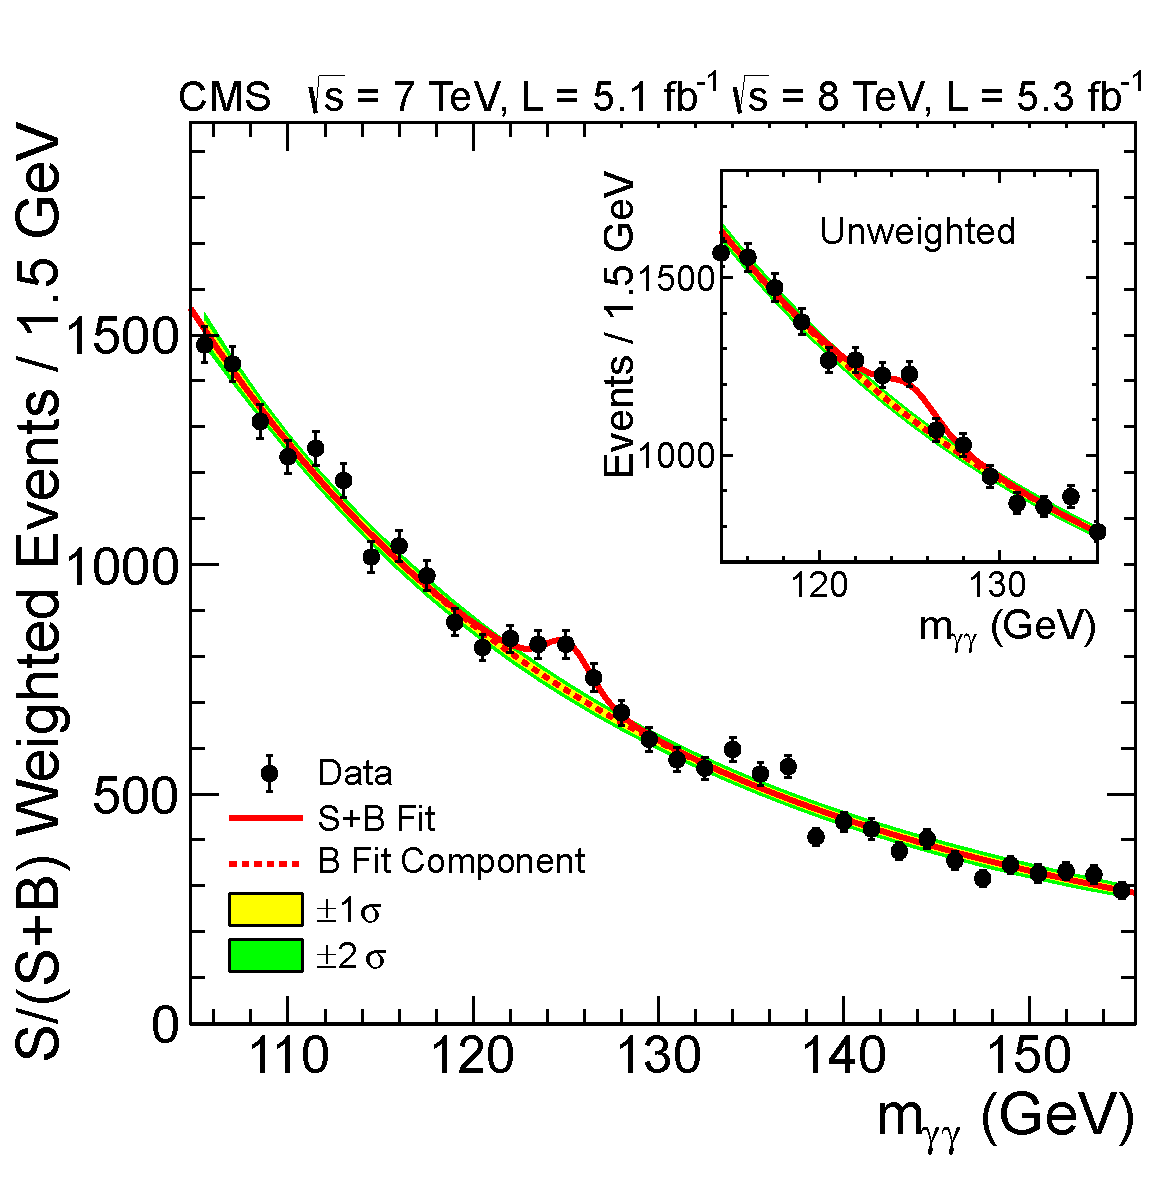
\includegraphics[width=0.49\columnwidth]{figures_chapter2/gammagamma}
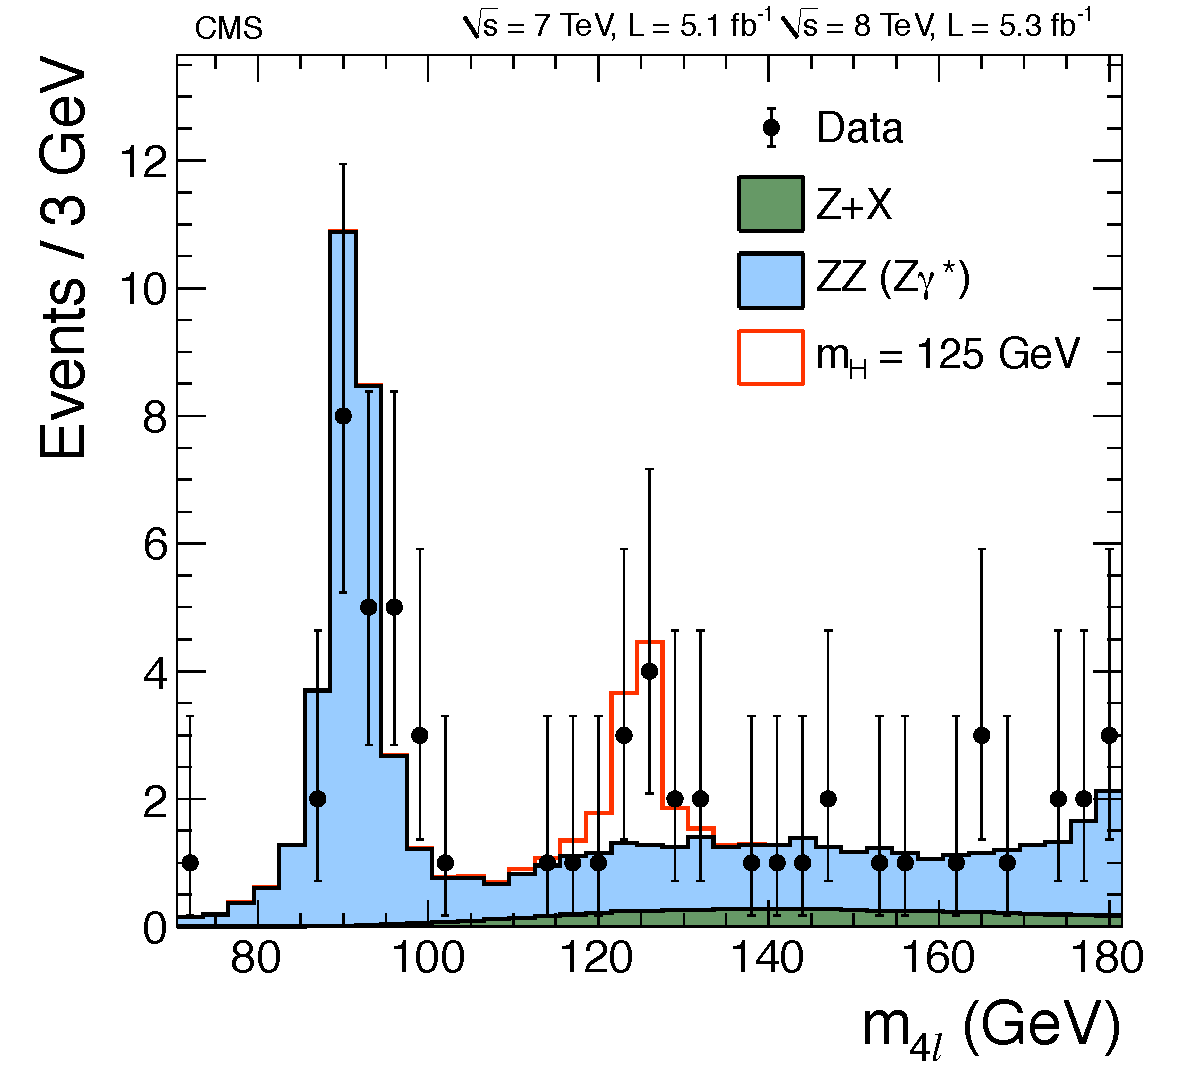
\includegraphics[width=0.49\columnwidth]{figures_chapter2/zz4l}
\caption{Distributions of the diphoton invariant mass with each event weighted by $S/(S+B)$ value (left panel) and the four-lepton invariant mass for the $ZZ \rightarrow 4 \ell$ decays (right panel)~\cite{Chatrchyan:2012xdj}.}
\label{fig:cms_higgs}
\end{figure}

The search for the SM Higgs boson has been one of the highlights of the Large Hadron Collider (LHC)~\cite{1748-0221-3-08-S08001}. In July 2012, the ATLAS and CMS collaborations announced the observation of a narrow resonance with a mass of about $125~\GeV$ with properties consistent with the SM Higgs boson~\cite{Aad:2012tfa,Chatrchyan:2012xdj}. Significant excesses were observed in $\gamma\gamma$ and $ZZ$ decay modes with rates consistent with the SM predictions. There were also strong hints in the data that the new particle decays to $W^+W^-$. The observed decay channels indicate that the new particle is a boson. Figure~\ref{fig:cms_higgs} shows the distributions of the diphoton invariant mass (weighted by the signal-to-background ratio) and four-lepton invariant mass for the $ZZ \rightarrow 4\ell$ decays from the CMS results. The ATLAS and CMS continued to take data after the discovery announcement. Subsequent measurements of the Higgs boson production and decay rates combining the ATLAS and CMS results with proton-proton collisions at centre-of-mass energies of $7$ and $8~\TeV$ show a consistent picture with the SM Higgs predictions~\cite{Khachatryan:2016vau}. The combined measurement measured mass of the discovered boson is $m_{H}=125.09 \pm 0.21 \mathrm{(stat.)} \pm 0.11 \mathrm{(syst.)}~\GeV$~\cite{Aad:2015zhl}. The spin and CP properties of the new boson are also consistent with those expected of the SM Higgs boson~\cite{Chatrchyan:2012jja,Aad:2013xqa,Khachatryan:2014kca}.

The measurement of the Higgs boson decays to $b\bar{b}$ and $\tau^{+}\tau^{-}$ is essential for identifying if the new boson is the SM Higgs boson. Both decay modes provide a direct probe of the Higgs Yukawa coupling to fermions. The $\tau^{+}\tau^{-}$ decay mode is currently the most promising channels to study the SM Higgs boson coupling to leptons.

\section{Overview of the Standard Model}

\subsection{Quantum Chromodynamics}

The gauge group of the strong interactions of the colored quarks and gluons is $SU(3)$. The most general gauge invariant and renormalizable Lagrangian of the quantum chromodynamics (QCD) is given by:

 \begin{equation} \label{eq:qcd_lang}
\mathcal{L} =  \bar{\psi}_{f,\alpha} (i \gamma^{\mu}\partial_{\mu}\delta_{\alpha\beta}-g_{s}\gamma^{\mu}t^{a}_{\alpha\beta}A^{a}_{\mu}-m_{f}\delta_{\alpha\beta})\psi_{f,\beta}-\frac{1}{4}F_{\mu\nu}^{b}F^{b,\mu\nu}-\theta\frac{g_{s}^2}{72\pi^2}\epsilon_{\mu\nu\rho\sigma}F^{c,\mu\nu}F^{c,\rho\sigma},
\end{equation}
where repeated indices are summed over. The $\psi_{f,\alpha}$ are the quark-field Dirac spinors of flavor $f$, color $\alpha$, and mass $m_{f}$. There are $6$ quark flavors, the up (u), charm (c), and top (t) each carrying an electric charge of $+2e/3$, and the down (d), strange (s), and bottom (b) each carrying an electric charge of $-e/3$. Each quark flavor comes in three "colors" transforming according to the fundamental representation of the $SU(3)$ color group. The $A_{\mu}^{a}$ denotes the massless gluon field vector potentials transforming according to the adjoint representation of the $SU(3)$ color group with $a$ running from $1$ to $N_{c}^2-1=8$ (8 gluons).  The $t_{\alpha\beta}^{a}$ are the eight generators of the color group represented by $3 \times 3$ Hermitian traceless matrices. The $g_{s}$ (or $\alpha_{s} = \frac{g_{s}}{4\pi}$) is the strong interaction coupling constant, the $\gamma^{\mu}$ are the Dirac matrices, and the gauge field tensor is given by:
 \begin{eqnarray} \label{eq:qcd_field}
 \begin{aligned}
F_{\mu\nu}^{a} &= \partial_{\mu}A_{\nu}^a-\partial_{\nu}A_{\mu}^a-g_{s}f_{abc}A_{\mu}^{b}A_{\nu}^{c},  \\
\mathrm{[}t^a,t^b\mathrm{]} &= if_{abc}t^{c},
\end{aligned}
\end{eqnarray}
where $f_{abc}$ are the structure constants of the $SU(3)$. The non-Abelian structure of the $SU(3)$ group means that the Feynman rules of QCD involve 3-gluon and 4-gluon vertices in addition to the quark-antiquark-gluon vertex. The last term in the Lagrangian in Eq.~(\ref{eq:qcd_lang}) can induce an electric dipole moment for the neutron introducing a CP violation. However the experimental limits on the electric dipole moment constrain the $\theta$ parameter to be smaller than $10^{-10}$~\cite{Agashe:2014kda}. This is known as the strong CP problem with a possible resolution given by the Peccei-Quinn theory predicting the existence of a hypothetical particle Axion~\cite{PhysRevLett.38.1440}. There are $7$ fundamental parameters in QCD Lagrangian (not counting the $\theta$ parameter): the $6$ quark masses and the strong coupling $g_{s}$ constant.

Predictions utilizing perturbative QCD (pQCD) calculations are expressed in terms of the renormalized coupling $g_{s} (\mu_R)$ as a function of a non-physical renormalization scale $\mu_R$. The renormalization group equation to three-loop order is given by:
\begin{eqnarray} \label{eq:qcd_rge}
\mu\frac{d}{d\mu}g_s{\mu_R} = - (\beta_{0} \frac{g_{s}^{3}(\mu_R)}{16\pi^2} +  \beta_{1} \frac{g_{s}^{5}(\mu_R)}{128\pi^4} + \beta_{2} \frac{g_{s}^{7}(\mu_R)}{8192\pi^6}),
\end{eqnarray}
where the loop coefficients $\beta_{i}$ are:
\begin{eqnarray} \label{eq:qcd_beta}
\begin{aligned}
\beta_{0}&=11-\frac{2}{3}n_{f}, \\
\beta_{1}&=51-\frac{19}{3}n_{f}, \\
\beta_{2}&=2857-\frac{5033}{9}n_{f}-\frac{325}{27}n_{f}^2,
\end{aligned}
\end{eqnarray}
and $n_{f}$ is the number of quark flavors with masses below the energies of interest~\cite{Agashe:2014kda}. The minus sign in Eq.~(\ref{eq:qcd_rge}) is the source of the asymptotic freedom and as can be seen in Eq.~(\ref{eq:qcd_beta}) the theory is asymptotically free as long as there are less than $16$ quark flavors below the energy scale of interest. Setting the renormalization scale near the momentum transfer $Q$ of a given process gives the effective strength of the strong coupling. Thus the strong coupling becomes weak for larger $Q$ and $\alpha_{s} \approx 0.1$ for momentum transfers near $100~\GeV$. Free quarks and gluons have not been observed experimentally. The asymptotic freedom implies that the strong coupling increases at low energies (large distances) and only color-singlet combinations of quarks, massless gluons, and anti-quarks, referred as hadrons, can be observed.  
 
\subsection{Electroweak Model}

The gauge group of the electroweak interactions is $SU(2) \times U(1)$ with the corresponding gauge bosons $\vec{W}_{\mu}$ and $B_{\mu}$ respectively. The $SU(2)$ part of the gauge group is chiral acting only on the left-handed components of the quark and lepton fields. The left handed fermion fields transform as doublets under $SU(2)$ given by:
\begin{eqnarray} \label{eq:doublet}
\Psi  = \left(\begin{array}{c} \nu_{f}\\ \ell_{f} \end{array} \right)\mathrm{,}  \quad \left(\begin{array}{c} \nu_{\mu}\\ \mu \end{array} \right)\mathrm{,}   \quad \left(\begin{array}{c} \nu_{\tau}\\ \tau \end{array} \right),
\end{eqnarray}   
for each lepton generation and by:
\begin{eqnarray} \label{eq:doublet_quark}
\Psi  = \left(\begin{array}{c} u \\ d^{'} \end{array} \right)\mathrm{,}  \quad \left(\begin{array}{c} c\\ s^{'} \end{array} \right)\mathrm{,}   \quad \left(\begin{array}{c} t\\ b^{'} \end{array} \right),
\end{eqnarray}   
for the three quark flavors. The $d^{'}$, $s^{'}$, and $b^{'}$ are given by:
\begin{eqnarray} \label{eq:doublet_quark}
\begin{aligned}
d^{'} &= V_{ud}d + V_{us}s + V_{ub}b, \\
s^{'} &= V_{cd}d + V_{cs}s + V_{cb}b, \\
b^{'} &= V_{td}d + V_{ts}s + V_{tb}b, 
\end{aligned}
\end{eqnarray}   
where $V$ is the unitary Cabibbo-Kobayashi-Maskawa (CKM) mixing matrix~\cite{Cabibbo:1963yz,Kobayashi:1973fv}. The right handed fermion fields are $SU(2)$ singlets. The most general gauge invariant and renormalizable Lagrangian for the fermion fields $\psi_{i}$ is given by:

\begin{equation} \label{eq:ewk_ym}
\mathcal{L} = \sum_{i} \bar{\psi}_{i} \gamma^{\mu}(i \partial_{\mu}-\frac{g^{'}}{2}YB_{\mu}) \psi_{i}  - \bar{\Psi}_{i}\gamma^{\mu}\frac{g}{2}\vec{\sigma}\cdot\vec{W}_{\mu}\Psi_{i} - \frac{1}{4}\vec{W}_{\mu\nu}\cdot\vec{W}^{\mu\nu} - \frac{1}{4} B_{\mu\nu} B^{\mu\nu},
\end{equation}
where $g^{'}$ and $g$ are the gauge coupling constants of the $U(1)$ and $SU(2)$ respectively. Thus the $\frac{Y}{2}$, where $Y$ is the weak hypercharge, and the $\frac{1}{2}\vec{\sigma}$, where $\sigma_{i}$ are the Pauli matrices, are the generators of the $U(1)$ and $SU(2)$ respectively. The gauge field tensors are given by:
\begin{eqnarray} \label{eq:ewk_field}
\begin{aligned}
B_{\mu\nu} &= \partial_{\mu}B_{\nu}-\partial_{\nu}B_{\mu}  \\
\vec{W}_{\mu\nu} &=  \partial_{\mu}\vec{W}_{\nu}-\partial_{\nu}\vec{W}_{\mu} + g \vec{W}^{\mu} \times \vec{W}^{\nu}.
\end{aligned}
\end{eqnarray}
The hypercharge is normalized such that the electric charge $Q=\frac{1}{2}\sigma^3+\frac{Y}{2}$. The vector fields corresponding to particles with spin $1$ and definite mass are the charged $W^{\pm}_{\mu}$ bosons, the neutral $Z_{\mu}$ boson and the photon $A_{\mu}$ given in terms of the gauge fields as: 
\begin{eqnarray} \label{eq:bosons}
\begin{aligned}
A_{\mu} &= B_{\mu} \cos \theta + W_{\mu}^{3} \sin \theta \\
Z_{\mu} &= -B_{\mu} \sin \theta + W_{\mu}^{3} \sin \theta \\
W_{\mu}^{\pm} &= W^{1}_{\mu} \mp i W_{\mu}^{2},
\end{aligned}
\end{eqnarray}
where $\theta$ is the weak angle related to the gauge coupling constants by:
\begin{eqnarray} \label{eq:bosons}
\begin{aligned}
\sin \theta &= \frac{g^{'}}{\sqrt{g^2+g^{'2}}} \\
\cos \theta &= \frac{g}{\sqrt{g^2+g^{'2}}}.
\end{aligned}
\end{eqnarray}
However this theory of the electroweak interactions given in Eq.~(\ref{eq:ewk_ym}) is not satisfactory. It contains four massless bosons whereas only the photon is massless in nature. Attempting to add mass terms for the vector boson fields in the Lagrangian of the form $-M_{Z}^2Z_{\mu}Z^{\mu}$ breaks the gauge invariance. Furthermore introducing explicit mass terms for the spin-1 boson fields makes the theory non-renormalizable. There are also no mass terms in the Lagrangian for the fermion fields.  The Dirac fermion mass terms link the left and right-handed components of the fields:
\begin{eqnarray} \label{eq:fermion}
m\bar{\psi}\psi = m(\bar{\psi}_L\psi_R+\bar{\psi}_R\psi_L).
\end{eqnarray}
This breaks the symmetry as the left and right-handed components transform differently under the $SU(2)$ and $U(1)$. Spontaneous symmetry breaking mechanism leaving the underlying gauge symmetry intact was the solution to the conundrum on how the gauge bosons can acquire mass. 

\subsection{The SM Higgs mechanism}

Spontaneous symmetry breaking occurs when the ground state (vacuum) does not exhibit the symmetry of the theory. A key aspect is that the vacuum is degenerate and it can not be predicted in advance which state will be chosen. Taking a precedence from the superconductivity phenomenon it was reasoned that the gauge symmetry can be broken through spontaneous symmetry breaking~\cite{Nambu:1960tm,Anderson:1963pc}. The main difficulty was the appearance of the massless spin-$0$ Nambu-Goldstone bosons after the spontaneous symmetry breaking (the Goldstone theorem~\cite{Goldstone:1962es}) as no such particles are observed. Englert, Brout, Higgs, Guralnik, Hagen, and Kibble showed that the theorem does not apply to the gauge theories ~\cite{Englert:1964et,Higgs:1964ia,Higgs:1964pj,Guralnik:1964eu,Higgs:1966ev,Kibble:1967sv}.  Taking these ideas Weinberg and Salam completed the electroweak unification started by Glashow~\cite{Glashow:1961tr,Weinberg:1967tq,Salam:1968rm}. They also added the possibility to generate the fermion masses through the same spontaneous symmetry breaking. Finally it was proved by t'Hooft and Veltman that this model is renormalizable~\cite{tHooft:1972fi}. 

The $SU(2)$ symmetry is broken by introducing a scalar field (Higgs) in the spinor representation of the $SU(2)$ 
\begin{eqnarray} \label{eq:lang_higgs}
\Phi  = \frac{1}{\sqrt{2}}\left(\begin{array}{c} \sqrt{2}\phi^{+}\\ \phi_{0}+ia^{0} \end{array} \right),
\end{eqnarray}   
with four real degrees of freedom in the complex doublet and weak hypercharge of $Y=1$. The most general renormalizable Lagrangian of the scalar field consistent with $SU(2) \times U(1)$ is given by

\begin{equation} \label{eq:ewk_higgs}
\mathcal{L}_{\Phi} = (D_{\mu}\Phi)^{\dagger} (D^{\mu}\Phi) - \mu^2 \Phi^{\dagger}\Phi - \lambda (\Phi^{\dagger}\Phi)^2,
\end{equation}
with $\lambda>0$. The covariant derivative, given by
\begin{equation} \label{eq:higgs_cov}
D_{\mu}\Phi = (\partial_{\mu}+\frac{1}{2}ig\vec{\sigma}\cdot\vec{W}_{\mu}+\frac{1}{2}g^{'}YB_{\mu})\Phi,
\end{equation}
is responsible for the Higgs field couplings to the $\vec{W}_{\mu}$ and $B_{\mu}$ gauge fields. There is a tree-approximation non-zero vacuum expectation value (VEV) for $\mu^2<0$ given by

\begin{eqnarray} \label{eq:vev}
<\Phi>  =  \left(\begin{array}{c} 0\\ \frac{1}{\sqrt{2}}\nu \end{array} \right),
\end{eqnarray}    
with VEV $\nu^2= -\frac{\mu^2}{\lambda}$. A $SU(2)\times U(1)$ gauge transformation was performed in Eq.~(\ref{eq:vev}) to a unitary gauge in which $\phi^{+}=0$, and $a^{0}=0$ with $<\phi^{0}>0$. Defining $\phi^{0}=H+\nu$ in the Lagrangian in Eq.~(\ref{eq:ewk_ym}) induces the spontaneous breaking of the SM gauge symmetry $SU(2)\times U(1)$ into $U(1)_{em}$ group. The generator of the $U(1)_{em}$ gauge group is the electric charge $Q=\frac{1}{2}\sigma^3+\frac{Y}{2}$. Thus the photon field $A_{\mu}$ remains massless and the Higgs Lagrangian is given by

 \begin{eqnarray} \label{eq:ewk_higgs2}
 \begin{aligned}
\mathcal{L_{H}} &= \frac{1}{2} \partial_{\mu}H\partial^{\mu}H - \frac{1}{2} m_{H}^2 H^2 -\frac{1}{2}m_{W}^2W_{\mu}^{+}W^{-\mu} - \frac{1}{2}m_{Z}^2Z_{\mu}Z^{\mu}  \\
&+ \frac{m_{H}^2}{2\nu} H^3 + \frac{m_{H}^2}{8\nu^2} H^4 + \frac{m_{Z}^2}{\nu} Z_{\mu}Z^{\mu}H + \frac{2m_{W}^2}{\nu} W^{+}_{\mu}W^{-\mu} H  \\
&+ \frac{m_{Z}^2}{2\nu^2} Z_{\mu}Z^{\mu} H^2 +\frac{m_{W}^2}{\nu^2} W^{+}_{\mu}W^{-\mu} H^2,
\end{aligned}
\end{eqnarray}
where the Lagrangian is expressed in terms of the $W_{\mu}^{\pm}$ and $Z_\mu$ fields given in Eq.~(\ref{eq:bosons}) and
 \begin{eqnarray} \label{eq:masses}
 \begin{aligned}
m_{H}  &= \sqrt{-2\mu^2} \\
m_{W} &= \frac{1}{2}g\nu = \cos\theta m_{Z} \\
m_{Z} &= \frac{1}{2} \sqrt{g^2+g^{'2}}\nu \\
m_{A} &= 0.
\end{aligned}
\end{eqnarray}
Thus the spin-$1$ gauge bosons $W_{\mu}^{\pm}$ and $Z_\mu$ have acquired mass. The Higgs boson field H is also massive. The three scalar fields in Eq.~(\ref{eq:lang_higgs}) are "eaten" by the $W_{\mu}^{\pm}$ and $Z_\mu$ fields and the fourth remains as the neutral Higgs field. One can see that the Higgs boson couplings to the spin-$1$ vector bosons are proportional to the mass squared of the bosons. The Higgs boson trilinear and quartic self couplings are proportional to the $m_{H}^2$.

The final item to complete the theory is to add a mechanism for generating the fermion masses. The fermions acquire a mass through a Yukawa type interactions between the Higgs scalar field and the fermions. The Yukawa Lagrangian before the electroweak symmetry is given by:
\begin{eqnarray} \label{eq:yukawa}
\mathcal{L_{\mathrm{Y}}} = -h_{d_{ij}} \bar{q}_{L_{i}} \Phi d_{R_j}  - h_{u_{ij}} \bar{q}_{L_{i}} i\sigma^{2}\Phi^{*}d_{R_j} - h_{\ell_{ij}} \bar{\ell}_L \Phi e_{R_j} + \quad \mathrm{h.c.}, 
\end{eqnarray}   
where the $q_L$ ($\ell_L$) and $u_R$, $d_R$ ($e_R$) are the quark (lepton) $SU(2)$ doublets (singlets) and the $3\times3$ matrices are the couplings~\cite{Agashe:2014kda}. After the electroweal symmetry breaking and rotating to the fermion mass eigenstate basis the coupling matrices are diagonalized and the fermions acquire masses given by $m_{f} = \frac{h_f \nu}{\sqrt{2}}$. The Higgs to fermion coupling term becomes $\frac{m_{f}}{\nu}\bar{f}fH$. Thus the fermions have acquired mass and the Higgs coupling to fermions is proportional to the mass of the fermion in question. The Dirac neutrino masses can also be included in this framework if one considers the right handed neutrinos. It has to be noted that the fermion mass parameters have been replaced by the Yukawa couplings. Finally the Lagrangian for the fermion fields $\psi_{i}$ after the electroweak symmetry breaking reads:

\begin{eqnarray} \label{eq:lf}
\begin{aligned}
\mathcal{L_F} &= \sum_{i} \bar{\psi}_{i} (i\partial - m_{i} - \frac{m_{i}H}{\nu}) \psi_{i} -\frac{g}{2\sqrt{2}}\sum_{i}\bar{\Psi}_i \gamma^{\mu}(1-\gamma^5)(T^{+}W_{\mu}^{+} + T^{-} W_{\mu}^{-})\Psi_{i}  \\
& -e\sum_{i} Q_i \bar{\psi}_{i} \gamma^{\mu} \psi_i A_{\mu} - \frac{g}{2\cos\theta}\sum_{i}\bar{\psi}_i \gamma^{\mu}(g_{V}^{i}-g_{A}^{i}\gamma^{5})\psi_{i}Z_{\mu}, 
\end{aligned}
\end{eqnarray}
where $e=g \sin \theta$ is the magnitude of the electron electric charge. The vector and axial-vector couplings are given as $g_{A}^{i}=t^{i}_{3}$ and $g_{V}^{i}=t^{i}_{3}-2Q^{i} \sin^{2} \theta$, where the  $t^{i}_{3}$ is the weak isospin of fermion $i$. The $T^{\pm}$ are the weak isospin raising and lowering operators. The source of the CP violation in the Lagrangian is encoded in the CKM matrix.

It is interesting to consider the number of free parameters in the SM not considering the neutrino masses. There are $9$ Yukawa couplings for each fermion. The CKM matrix is unitary and thus has $4$ parameters. The $3$ coupling constants for each gauge component: $g_s$, $g$, $g^{'}$. The vacuum expectation value ($\nu$) and the self coupling $\lambda$ of the Higgs field, and the $\theta$ in the QCD Lagrangian are the remaining parameters. Thus there are $19$ free parameters in the SM theory of elementary particles. 

\subsection{Extended Higgs Sector}

The SM theory of elementary particles has been remarkably successful in describing the present experimental observations. However there are number of undesirable aspects of the theory necessitating an effort to better understand the nature. The large number of free parameters in the model ($19$), the strong CP problem, the naturalness problem, the inclusion of gravity in the SM, understanding the generation of the neutrino masses are few examples to consider. There is also no candidate for the non-baryonic dark matter in the SM. 

The SM Higgs boson is a scalar particle and is therefore susceptible to the ultraviolet (UV) divergent radiative quadratic loop corrections. For example a Dirac fermion loop introduces a correction to the Higgs boson mass given by:
\begin{eqnarray} \label{eq:hierarchy}
m^{2}_{SM} = m^2_{\mathrm{bare}} - \frac{|\lambda_f|^2}{16\pi^2} \Lambda^2, 
\end{eqnarray}
where the $\lambda_f$ is the Yukawa coupling and $\Lambda$ is the ultraviolet cut-off scale. If the cut-off scale is at the Planck scale of $~10^{19}~\GeV$  then dramatic cancellations (fine tuning) are required on the right side of the Eq.~(\ref{eq:hierarchy}) to achieve a Higgs mass of the order of the electroweak scale. Supersymmetry is one of the proposed solutions to this naturalness problem~\cite{Golfand:1971iw,Wess:1974tw} where one introduces a new symmetry in nature between the bosons and fermions. A detailed introduction to the supersymmetry can be found in~\cite{Martin:1997ns}. The quadratic corrections to the Higgs mass have opposite signs for the fermion and boson loop corrections. In supersymmetry theories every SM fermion (boson) has a super-partner boson (fermion) providing a natural cancelation of the quadratic loop divergences. The supersymmetry is a broken symmetry as there are no hints of the super-partners in the experimental data. The naturalness problem is still a concern if the scale at which the symmetry breaks is larger than $1~\TeV$.  

The Minimal Supersymmetric Standard Model (MSSM) is the simplest extension of the SM to include the supersymmetry~\cite{Fayet:1974pd,Fayet:1977yc}. The Higgs sector in the MSSM considers an additional scalar Higgs doublet (2HDM) with hypercharge of $Y=-1$ given by:
 
\begin{eqnarray} \label{eq:2hdm}
\Phi_1  = \frac{1}{\sqrt{2}}\left(\begin{array}{c} \phi^{0}_1+ia_1^0 \\ \sqrt{2}\phi^{-}_1 \end{array} \right), \quad \Phi_2  = \frac{1}{\sqrt{2}}\left(\begin{array}{c} \sqrt{2}\phi^{+}_2 \\ \phi^{0}_2+ia_2^0 \end{array} \right).
\end{eqnarray}    
Analogous to the SM case, the scalar fields acquire vacuum expectation values as the electroweak symmetry is spontaneously broken. There are eight degrees of freedom in the 2HDM leading to five physical Higgs particles after the electroweak symmetry breaking:
\begin{eqnarray} \label{eq:mssm_higgs}
\begin{aligned}
H^{\pm} &= \sin \beta \phi_1^{\pm} + \cos \beta \phi_2^{\pm} \\
A  &= \sin \beta \mathrm{Im}\phi_1^{0} + \cos \beta \mathrm{Im}\phi_2^{0} \\
H  &= \cos \alpha(\mathrm{Re}\phi_1^{0}-\nu_1) + \sin \alpha (\mathrm{Re}\phi_2^{0}-\nu_2) \\
h  &= -\sin \alpha(\mathrm{Re}\phi_1^{0}-\nu_1) + \cos \alpha (\mathrm{Re}\phi_2^{0}-\nu_2),
\end{aligned}
\end{eqnarray}   
where $\nu_i=<\phi_i^0>$ are the vacuum expectation values satisfying the requirement $\nu_{SM}^2 = \nu_1^2 + \nu_2^2$. Thus there are two neutral CP-even states $h$ and $H$, and one neutral CP-odd state $A$. There is also a charged Higgs pair $H^{\pm}$. The mixing angle is related to the ratio of the vacuum expectation values $\tan \beta = \frac{\nu_2}{\nu_1}$. The $h$ ($H$) denotes the light (heavy) CP-even Higgs. The couplings of the $H$ and $A$ bosons to the down type quarks and leptons has an additional factor of about $\tan \beta$ enhancing the decay of the heavy neutral bosons to down type fermions for large $\tan \beta$.

At tree level the MSSM Higgs sector is determined by two parameters: $\tan \beta$ and the mass of one of the Higgs bosons ($m_{A}$ is typically chosen). The mass spectrum is given by:

\begin{eqnarray} \label{eq:mssm_mass}
\begin{aligned}
m_{H,h}^2 &= \frac{1}{2} (m_A^2 + m_Z^2 \pm \sqrt{(m_A^2+m_Z^2)^2-4m_Z^2m_A^2\cos^2_{2\beta}}), \\
m_{H^{\pm}}^2 &= m_{A}^2 + m_{W}^2.
\end{aligned}
\end{eqnarray}   

For $m_{A}$ much larger than the mass of the $Z$ boson (decoupling limit) the heavy scalars are almost degenerate $m_{H} \approx m_{H^{\pm}} \approx m_{A}$. There is also an upper bound on the lightest Higgs boson $m_{h} \leq m_{Z} \cos 2\beta$. However the radiative corrections are important and an upper bound of about $135~\GeV$ is possible~\cite{Degrassi:2002fi}. The strategy in interpreting the experimental results in the MSSM is to fix the parameters that enter through the radiative corrections (benchmark scenarios) and explore the parameter space in $m_{A}-\tan \beta$ plane. The discovery of the Higgs boson at mass of $125~\GeV$ invites to interpret the $h$ as the discovered boson and search for the heavier scalars appearing in the MSSM. Few benchmark scenarios are considered in the results~\cite{Heinemeyer:2011aa,Carena:2013ytb}.

\section{The Large Hadron Collider}
The LHC~\cite{1748-0221-3-08-S08001} is a circular proton-proton collider located at the European Organization for Nuclear Research (CERN). The tunnel has a circumference of $26.7$ km and previously hosted the Large Electron-Positron (LEP)~\cite{lep1,lep2} collider. Located at the border of France and Switzerland, the tunnel lies between $45$ m and $170$ m below the surface. The LHC is designed to collide beams of protons at centre-of-mass energy $\sqrt{s}$ of up to $14~\TeV$. While the LHC is primarily a proton-proton collider, lead (Pb) ion beams of energy of $2.3~\TeV$ per nucleon are used to produce lead-lead  and proton-lead collisions.  
 
Figure~\ref{fig:cern} shows a schematic representation of the accelerator complex at CERN. Ionized hydrogen atoms are accelerated to an energy of $50~\MeV$ in the Linac $2$ linear accelerator. Thereafter they are injected into the Proton Synchrotron Booster (PSB) and Super Proton Synchrotron (SPS) raising the energy to $25~\GeV$ and $450~\GeV$ respectively. From the SPS the protons are injected into two separate rings in discrete bunches. At the design bunch spacing of $25$ ns there are $2808$ proton bunches per beam. 

\begin{figure}[!h]
\centering
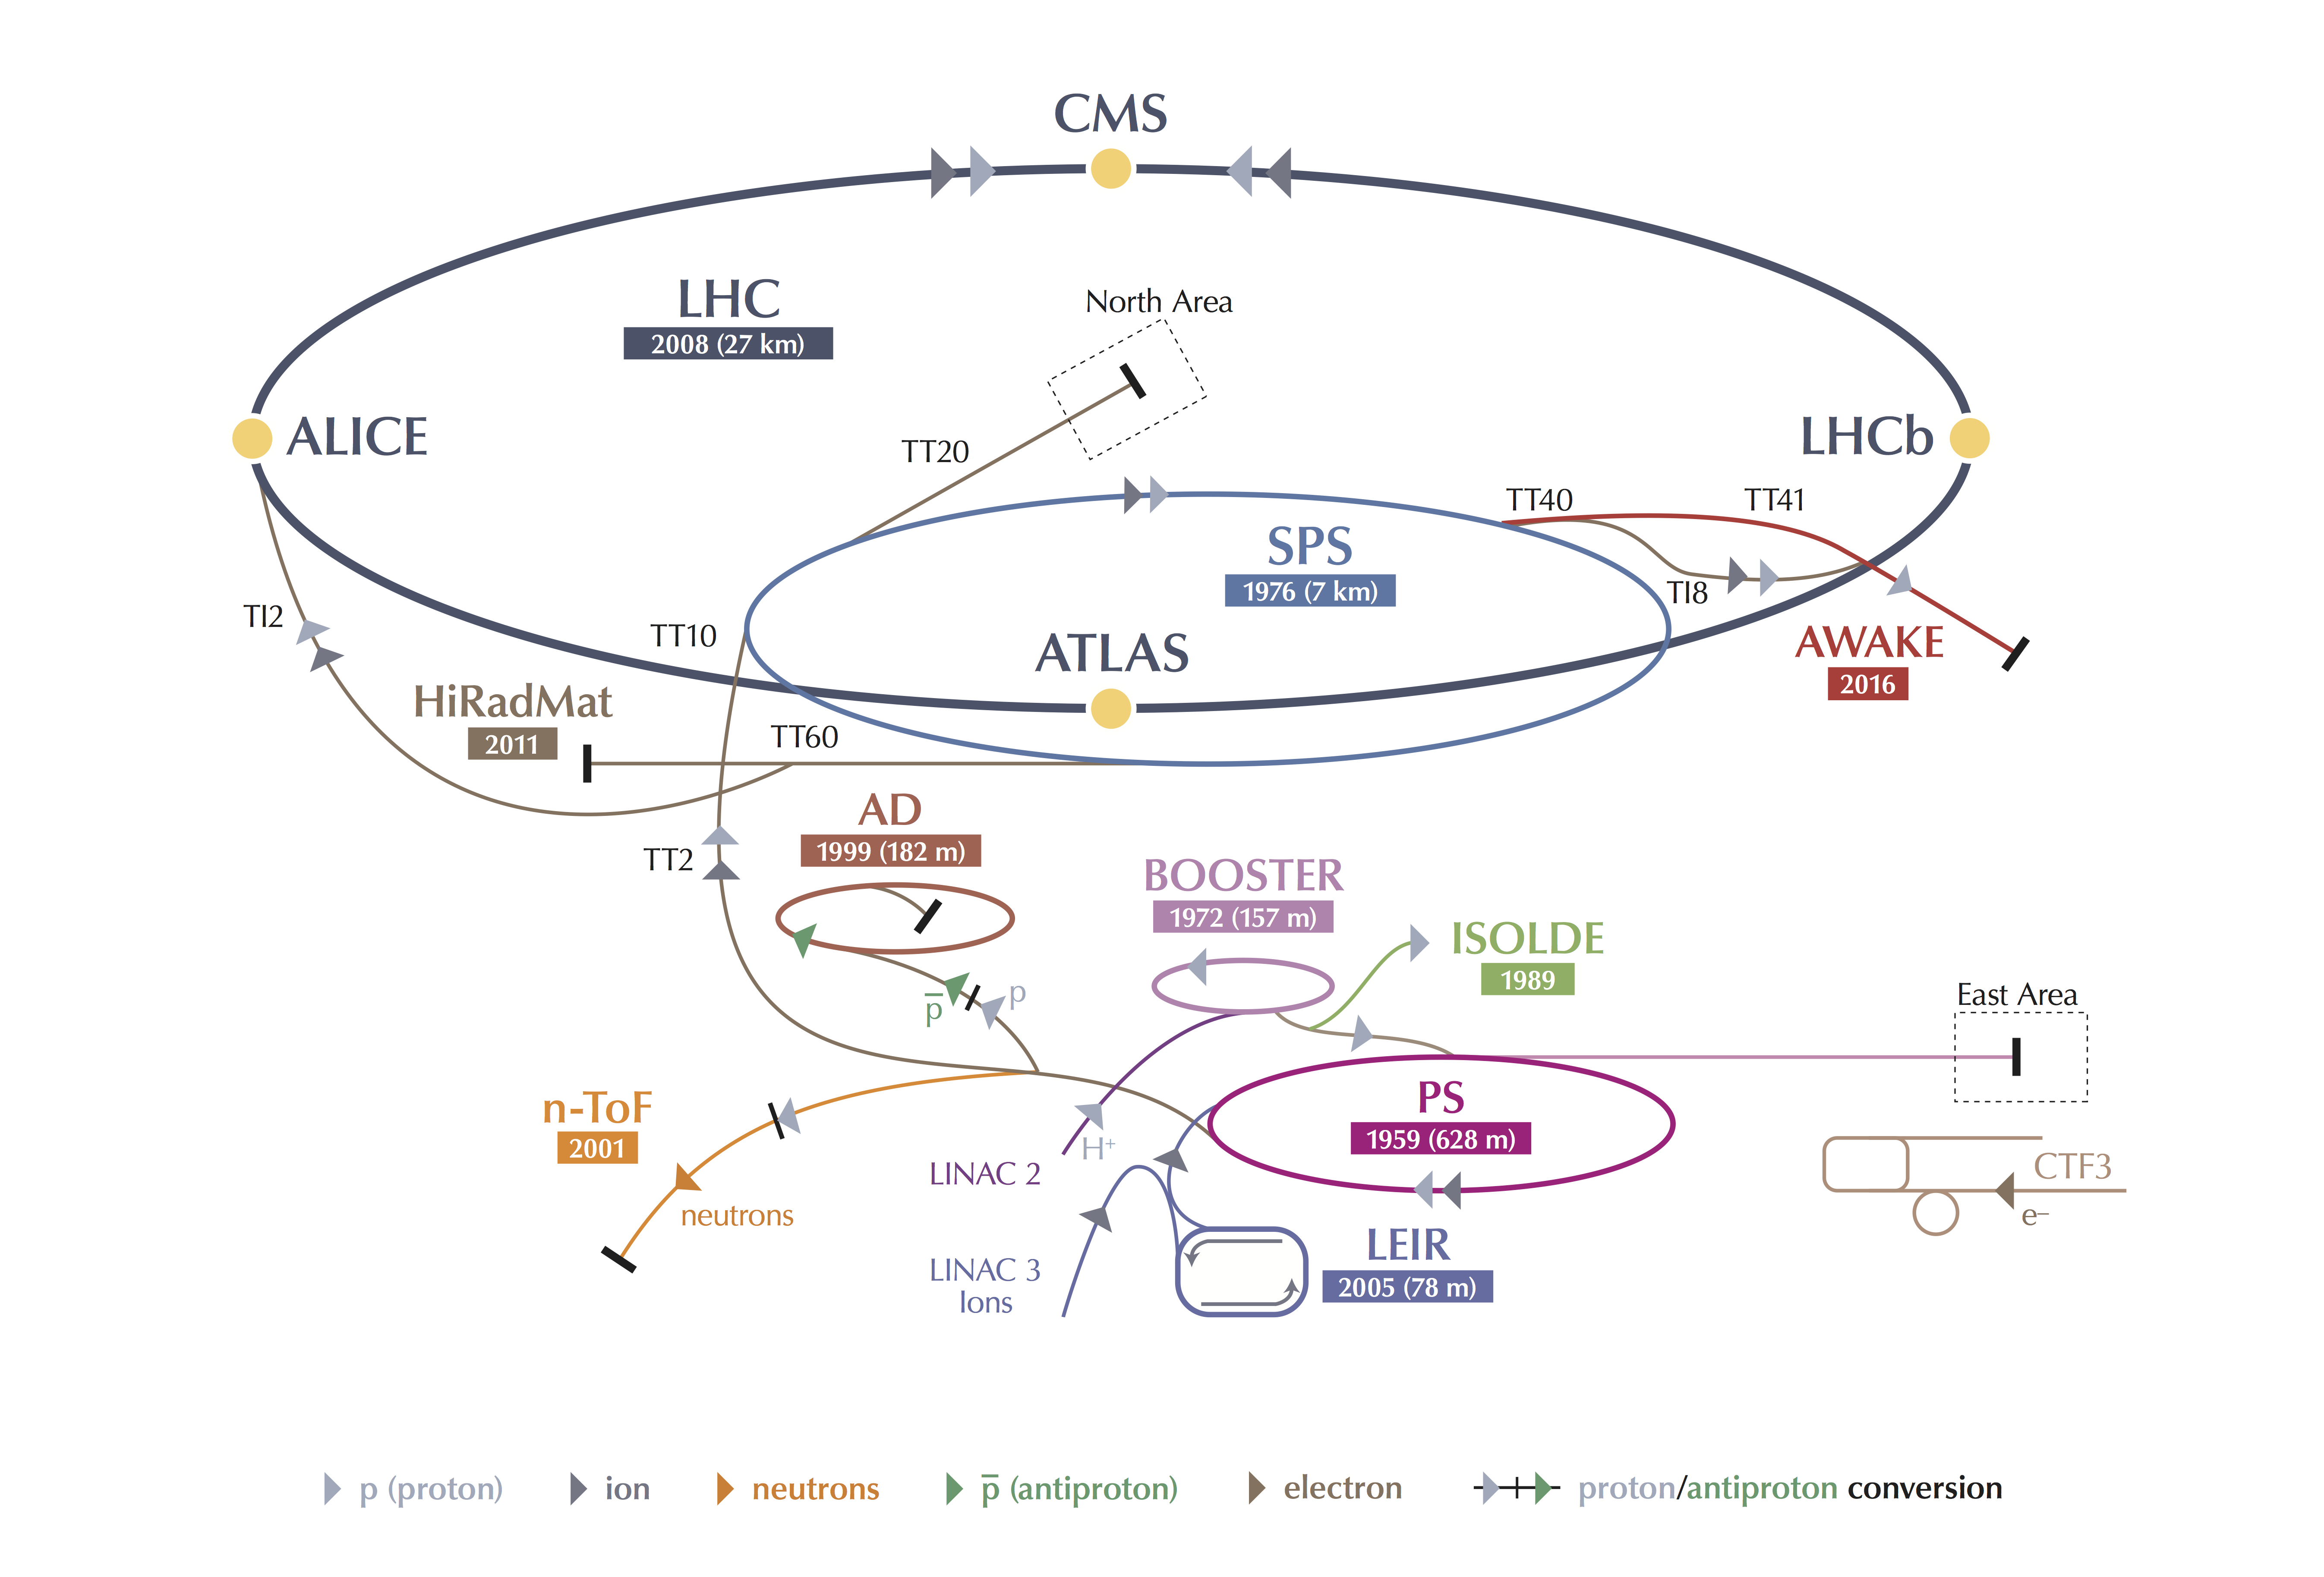
\includegraphics[width=1.0\columnwidth]{figures_chapter2/cern_complex.jpg}
\caption{A schematic representation of the CERN accelerator complex~\cite{Haffner:1621894}.}
\label{fig:cern}
\end{figure}

Using the synchrotron method the design beam energy is achieved with $1232$ dipole magnets (15 meters in length) with a peak dipole field of $8.33$ Tesla. Quadrupole magnets (492) of $5-7$ meters in length are used to focus the beams. Two beam pipes with counter rotating beams are required as the LHC is a particle-particle accelerator.  Space limitations in the tunnels led to the adoption of the twin-bore~\cite{Blewett:1971zzb} magnet design where the beam pipes are magnetically coupled and the magnets share the same mechanical structure and cryostat. The target magnetic field is achieved using niobium-titanium superconducting electromagnets with operating temperatures of $1.9$ K. Superfluid helium is used to cool the magnets to the operating temperature.   

\begin{figure}[!h]
\centering
%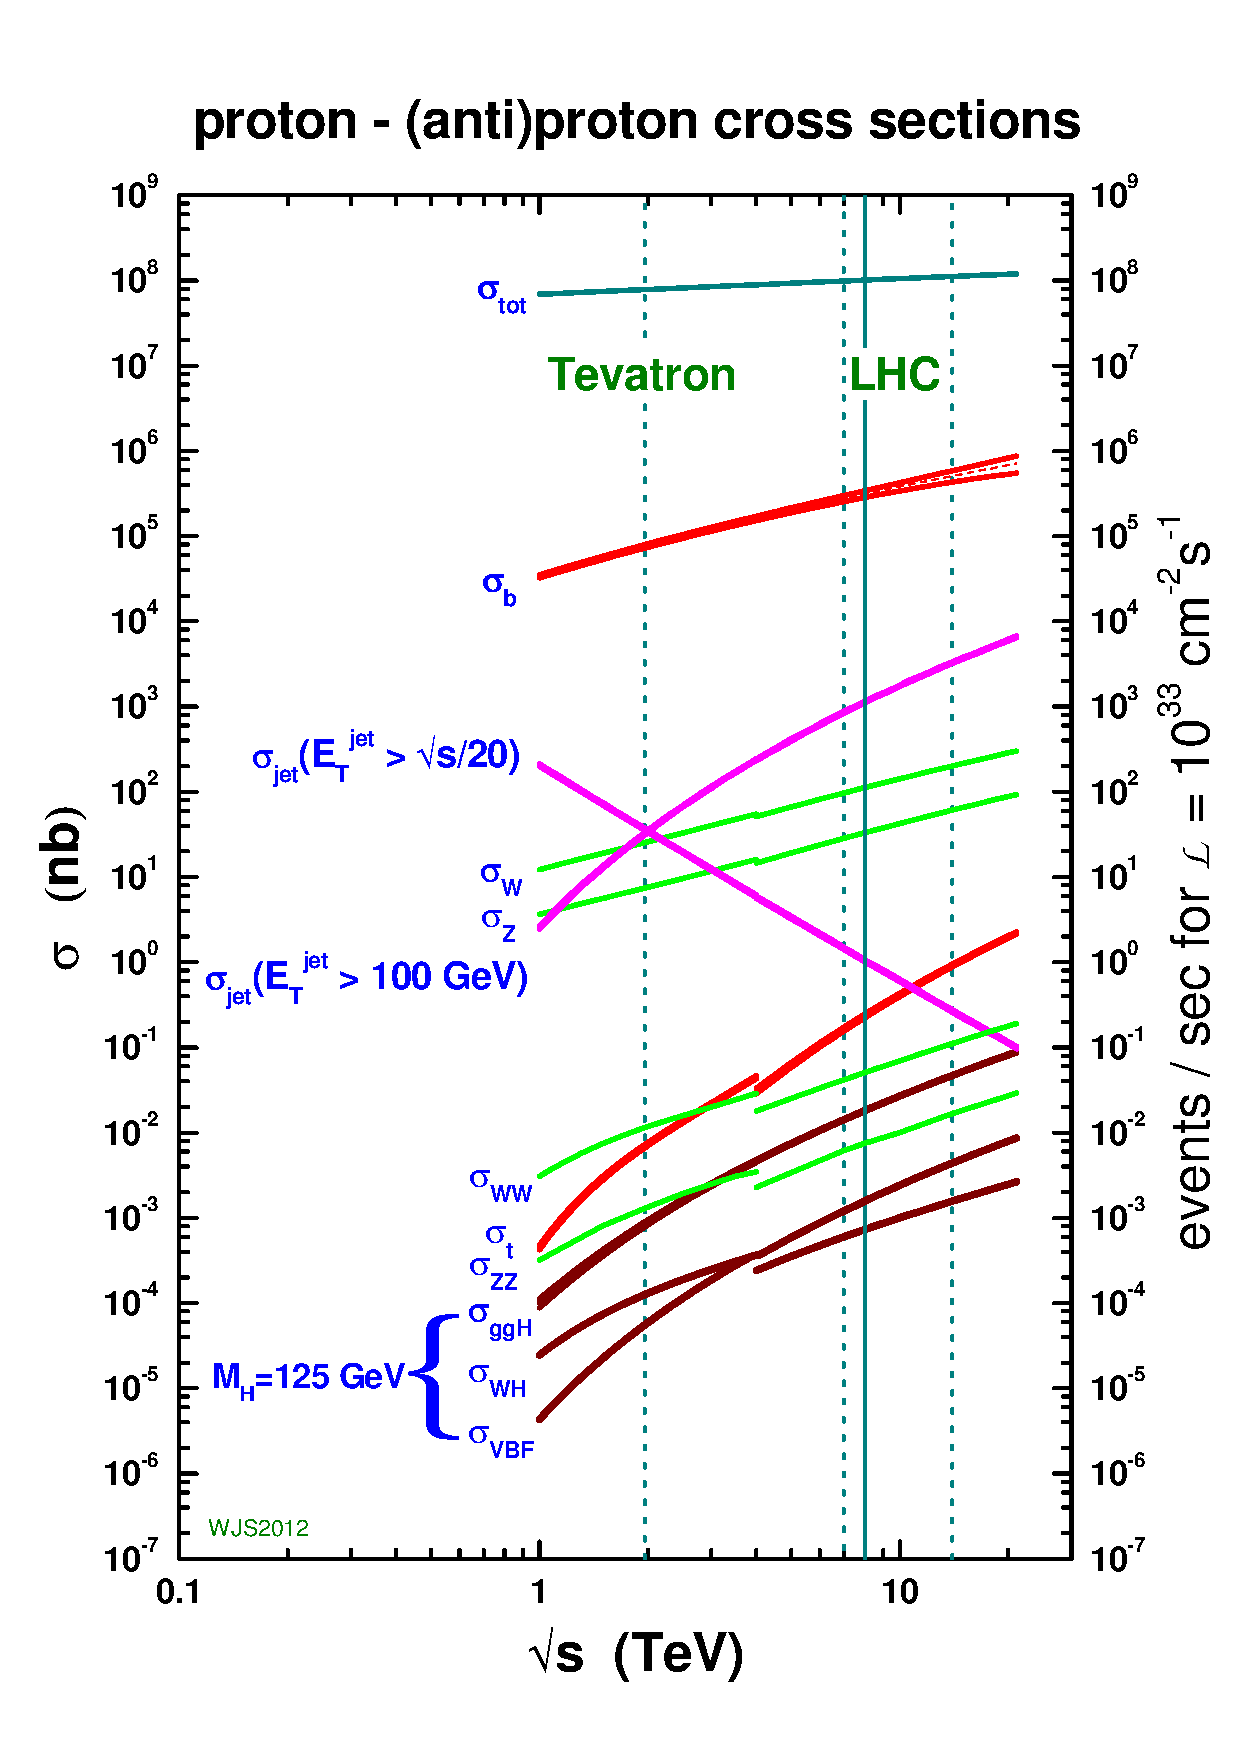
\includegraphics[width=1.0\columnwidth]{figures_chapter2/crosssections2013}
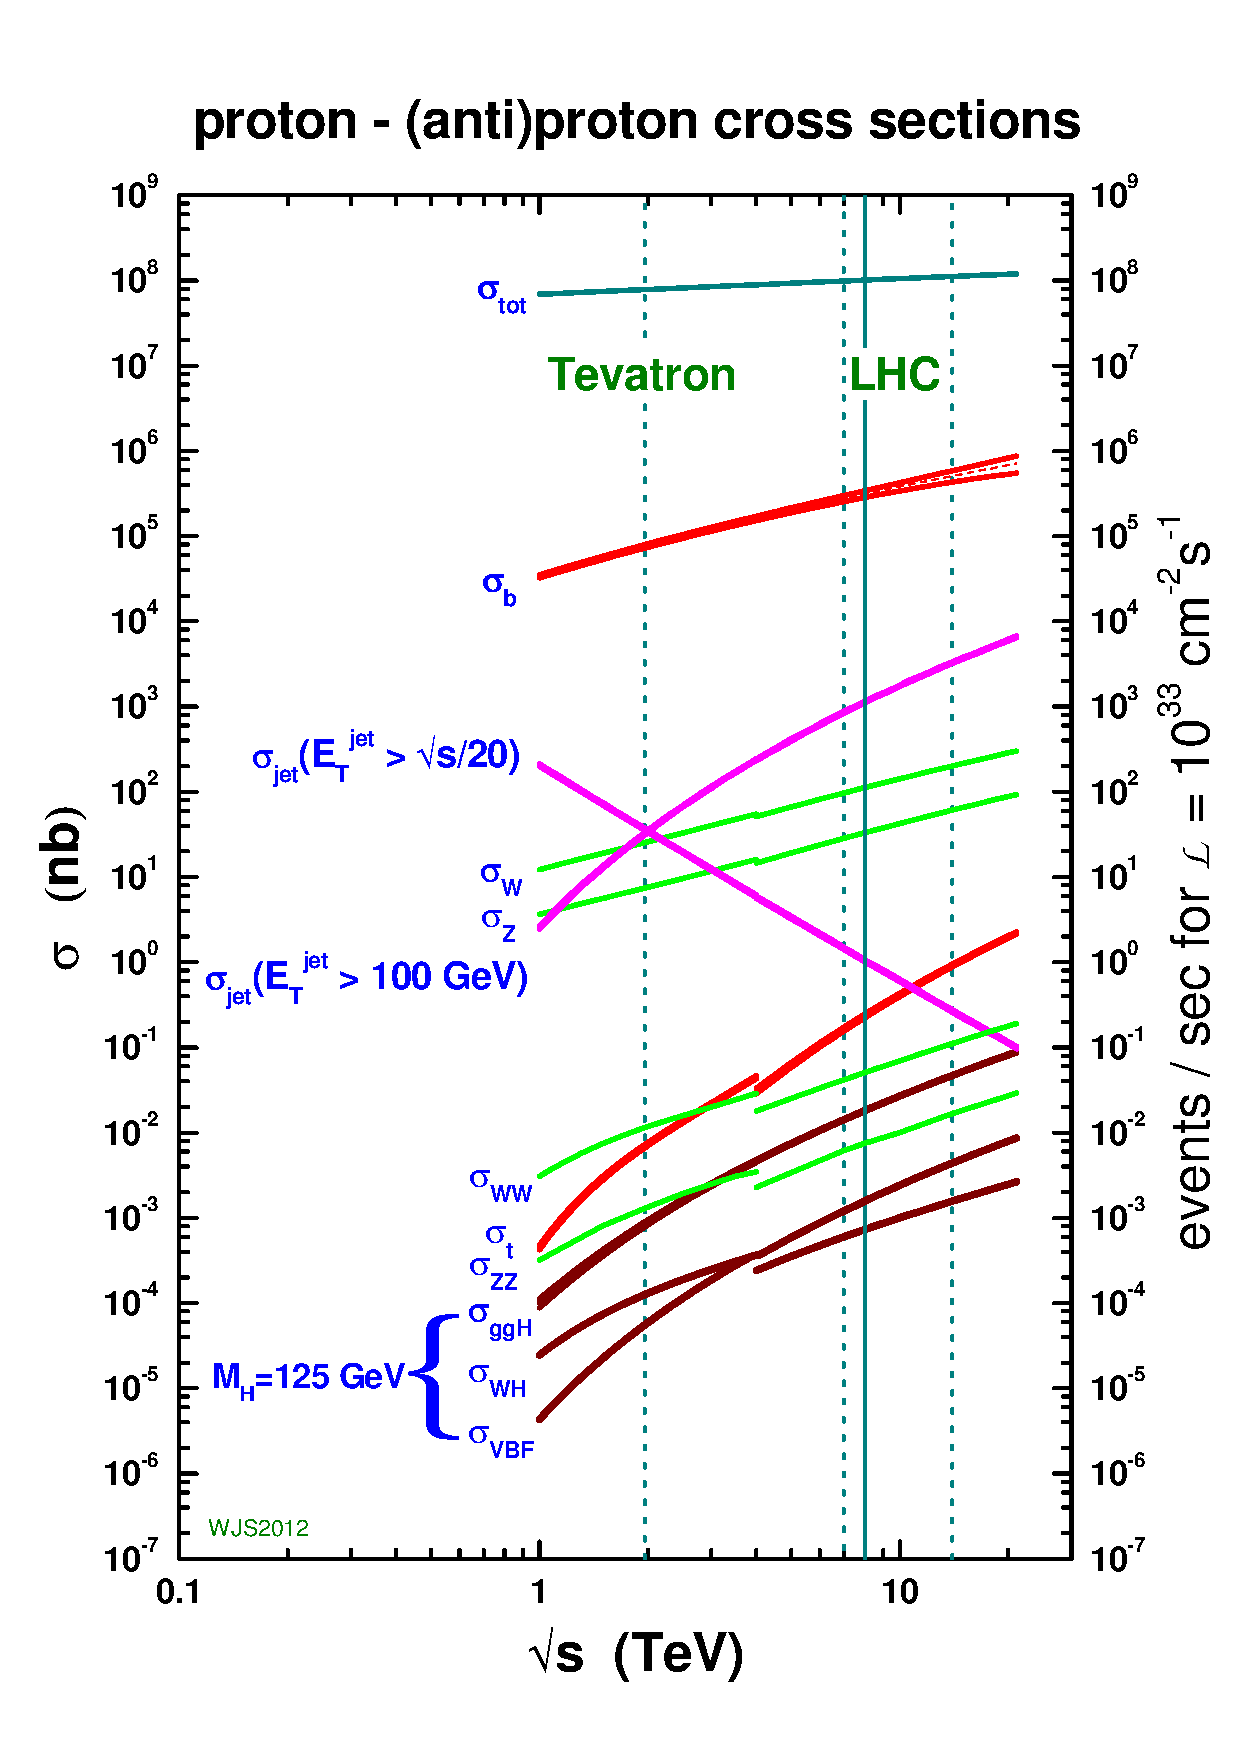
\includegraphics[width=0.6\columnwidth]{figures_chapter2/crosssections2013}
\caption{Cross sections of various SM processes as a function of $\sqrt{s}$ in proton-proton and proton-antiproton collisions~\cite{sterling}. The total hadronic cross section is based on a parameterization from Particle Data Group~\cite{Agashe:2014kda}. The remaining cross sections are calculated at NLO or NNLO using MSTW2008 parton distributions~\cite{MSTW}. The discontinuities illustrate the differences in cross sections between the proton-proton and proton-antiproton collisions.}
\label{fig:xsec}
\end{figure}

The goal of the LHC is to elucidate the mechanism of the electroweak symmetry breaking and to look for hints of beyond the Standard Model (BSM) physics. The rate of events generated in the LHC collisions is given by 
\begin{equation} \label{eq:lumi}
N = \sigma L,
\end{equation}
where $\sigma$ is the cross section of the event under study and $L$ is the luminosity. Figure~\ref{fig:xsec} shows the production cross sections of various SM processes as a function of $\sqrt{s}$ in proton-proton and proton-antiproton collisions. The rear processes of interest at the LHC are orders of magnitude smaller than the total hadronic cross section. Therefore, in addition to high beam energies, high beam intensities are required. The design peak luminosity at the LHC is $10^{34}$ cm$^2$s$^{-1}$ for the proton-proton collisions. The high beam intensity requirement excludes the feasibility of using proton-antiproton collisions at the LHC. 


\begin{figure}[!h]
\centering
%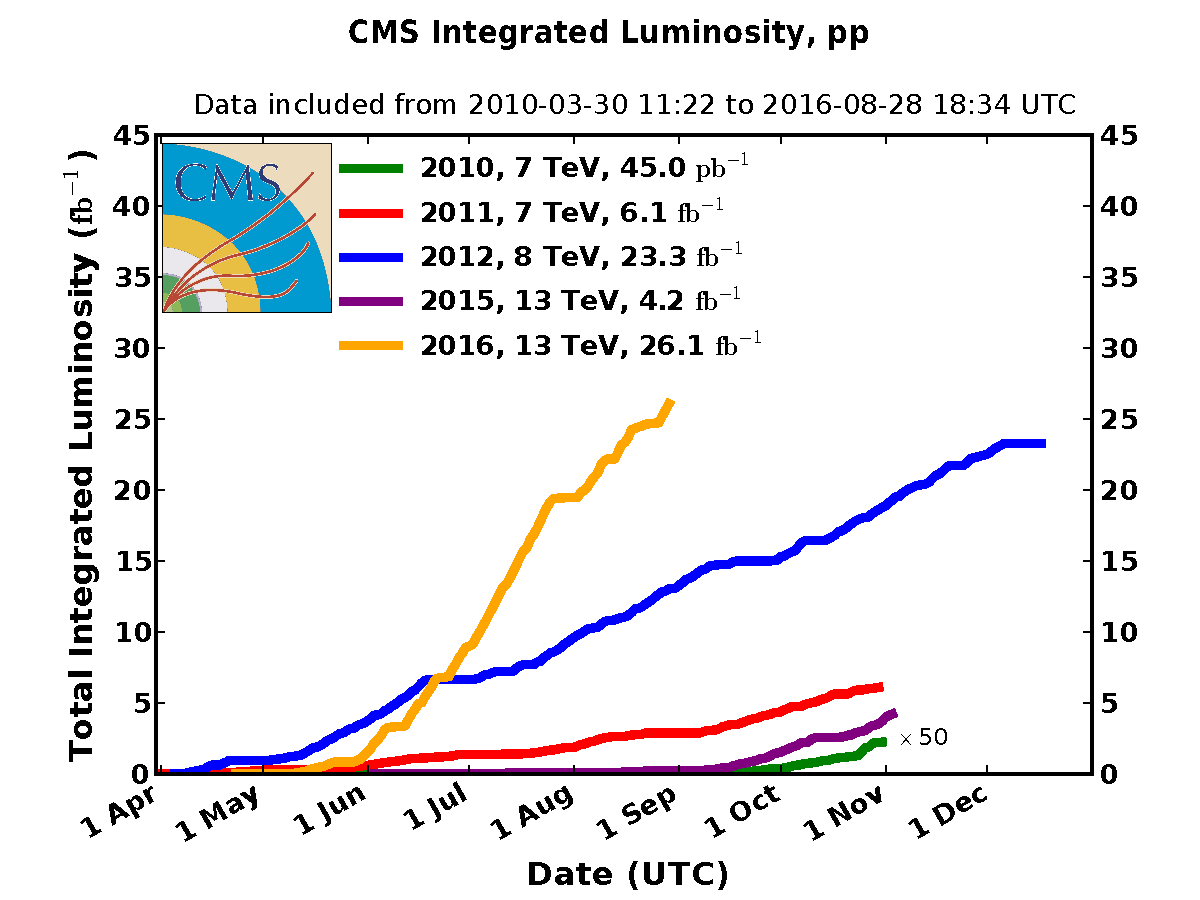
\includegraphics[width=1.0\columnwidth]{figures_chapter2/int_lumi_cumulative_pp_2}
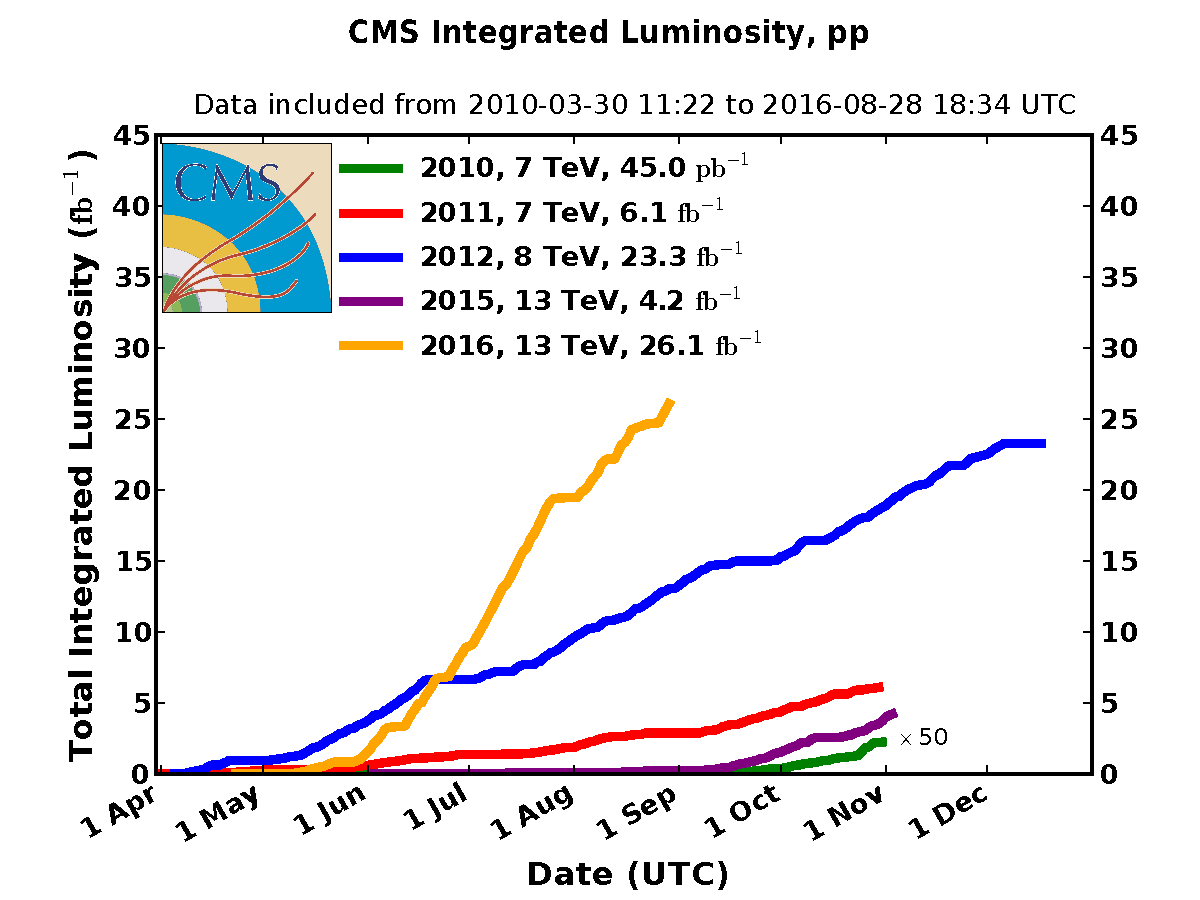
\includegraphics[width=0.8\columnwidth]{figures_chapter2/int_lumi_cumulative_pp_2}
\caption{The total integrated luminosity delivered to CMS during stable beams in proton-proton collisions~\cite{lumi_plot}. It is shown for $2010$ (green), $2011$ (red), $2012$ (blue), $2015$ (purple), and $2016$ (orange) data taking periods. The total integrated luminosity is shown for the data collected up to the end of August for the 2016 data taking period.} 
\label{fig:int}
\end{figure}

The machine luminosity depends only on the beam parameters. For a Gaussian beam distribution the dependance is given by
\begin{equation} \label{eq:lumi_beam}
L = \frac{N_{b}^2n_bf_{rev}\gamma_{r}}{4\pi\epsilon_n\beta^{*}}F,
\end{equation}
where $N_b$ is the number of particle per bunch ($\mathcal{O}(10^{11})$), $n_b$ is the number of bunches per beam, $f_{rev}$ is the revolution frequency, $\gamma_r$ is the relativistic gamma factor, $\epsilon_n$ is the normalized transverse beam emittance, $\beta^{*}$ is the beta function at the collision point, and $F$ is the geometric luminosity reduction factor due to the crossing angle at the interaction point.  The LHC has four interaction points that host ALICE~\cite{Aamodt:2008zz}, ATLAS~\cite{Aad:2008zzm}, CMS~\cite{Chatrchyan:2008aa}, and LHCb~\cite{Alves:2008zz} detectors. The ATLAS and CMS are general purpose, high luminosity experiments. The LHCb is a forward detector specializing in heavy flavor physics. The ALICE experiment is designed to study heavy-ion collisions.   

Figure~\ref{fig:int} shows the total integrated luminosity delivered to CMS during stable beams from October, $2010$ to August, $2016$ data taking periods. The LHC delivered proton-proton collisions at $\sqrt{s}$ of $7~\TeV$ during $2010$ and $2011$. The total integrated luminosity delivered in $2011$ was $6.1~\ifb$ with a peak instantaneous luminosity of $4.0 \times 10^{33}$ cm$^2$ s$^{-1}$. The luminosity recorded and certified, where all the detector sub-components are confirmed to operate normally, for physics results was $5.1~\ifb$. $\sqrt{s}$ was increased to $8~\TeV$ in $2012$ with $23.3~\ifb$ total integrated luminosity delivered to CMS with a peak instantaneous luminosity of $7.7 \times 10^{33}$ cm$^2$ s$^{-1}$. The total certified data amounted to $19.7~\ifb$. A bunch spacing of $50$ ns was used in the $2011$ and $2012$ data taking periods. 

 \begin{figure}[!h]
\centering
%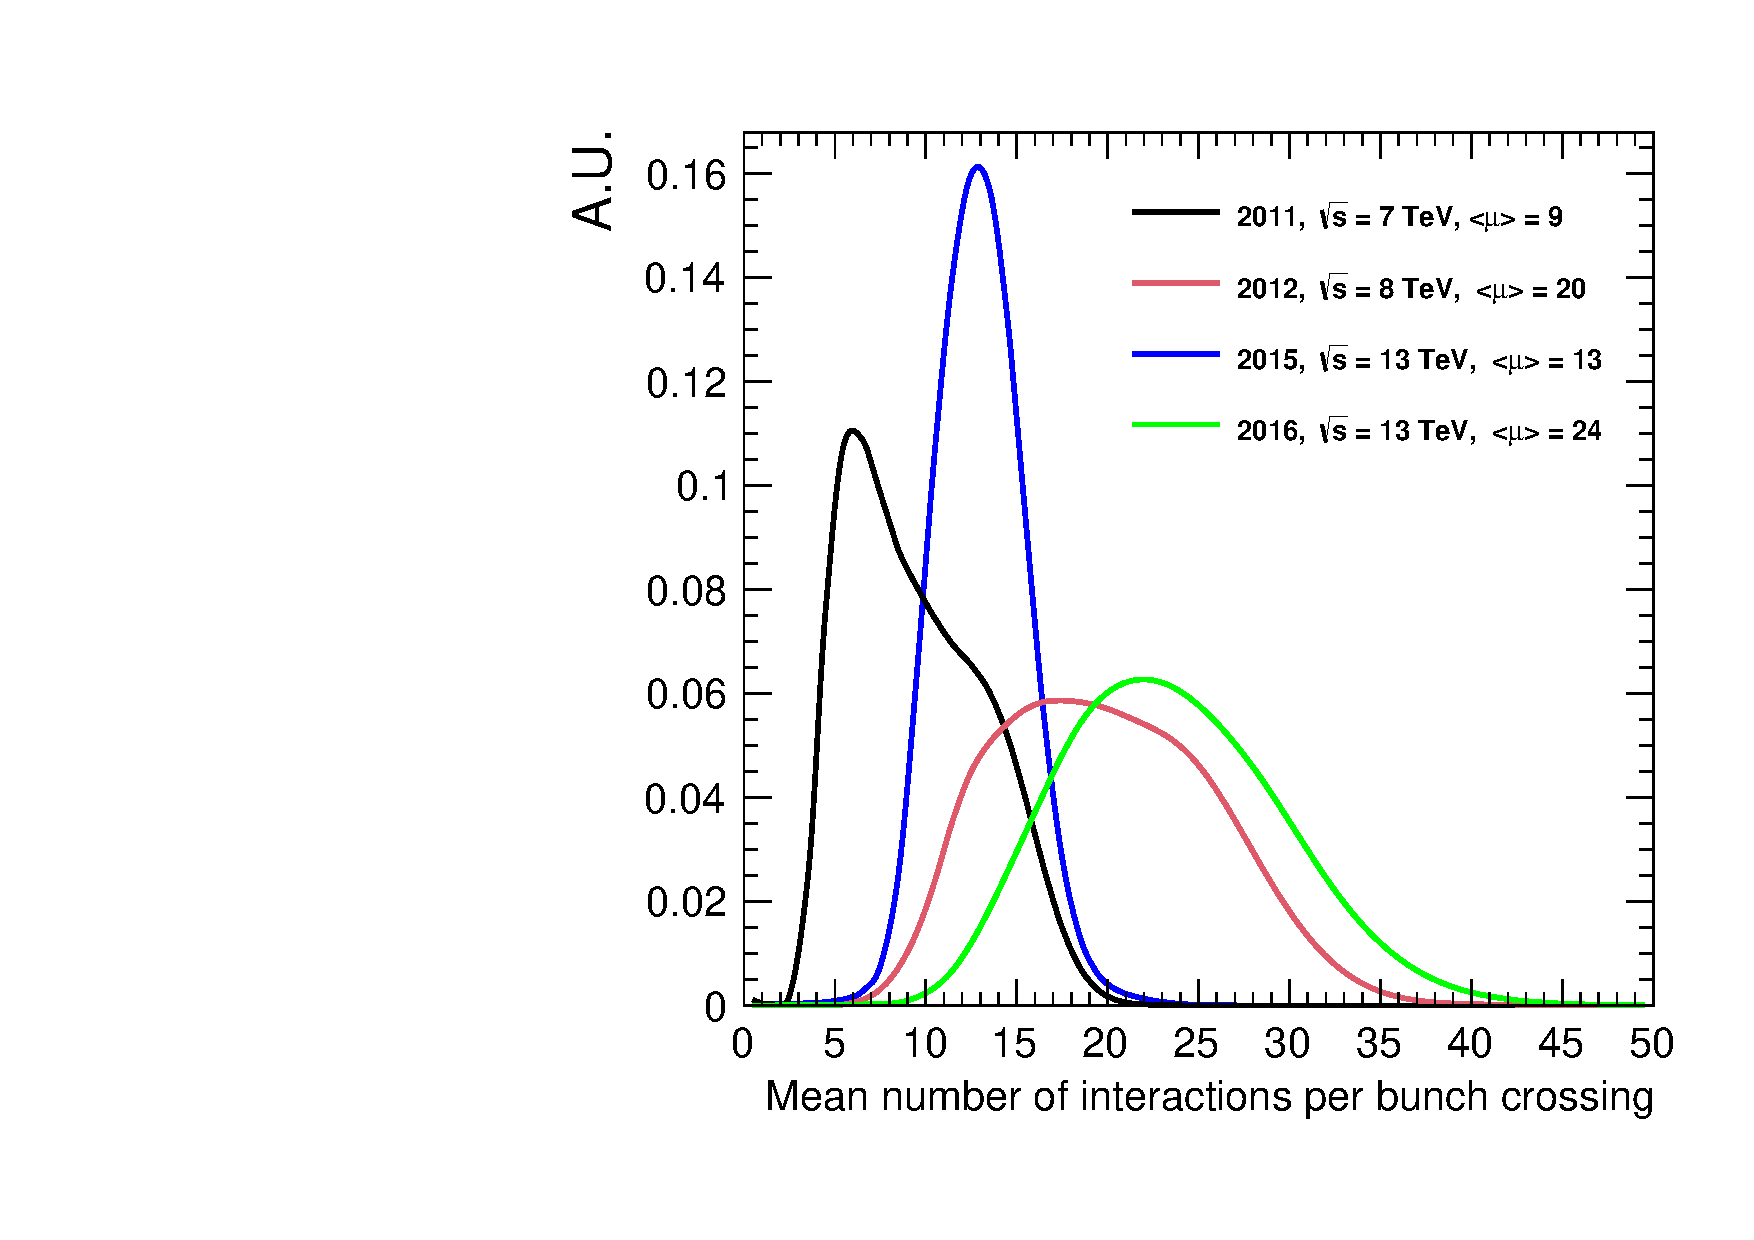
\includegraphics[width=1.0\columnwidth]{figures_chapter2/pileup_cms}
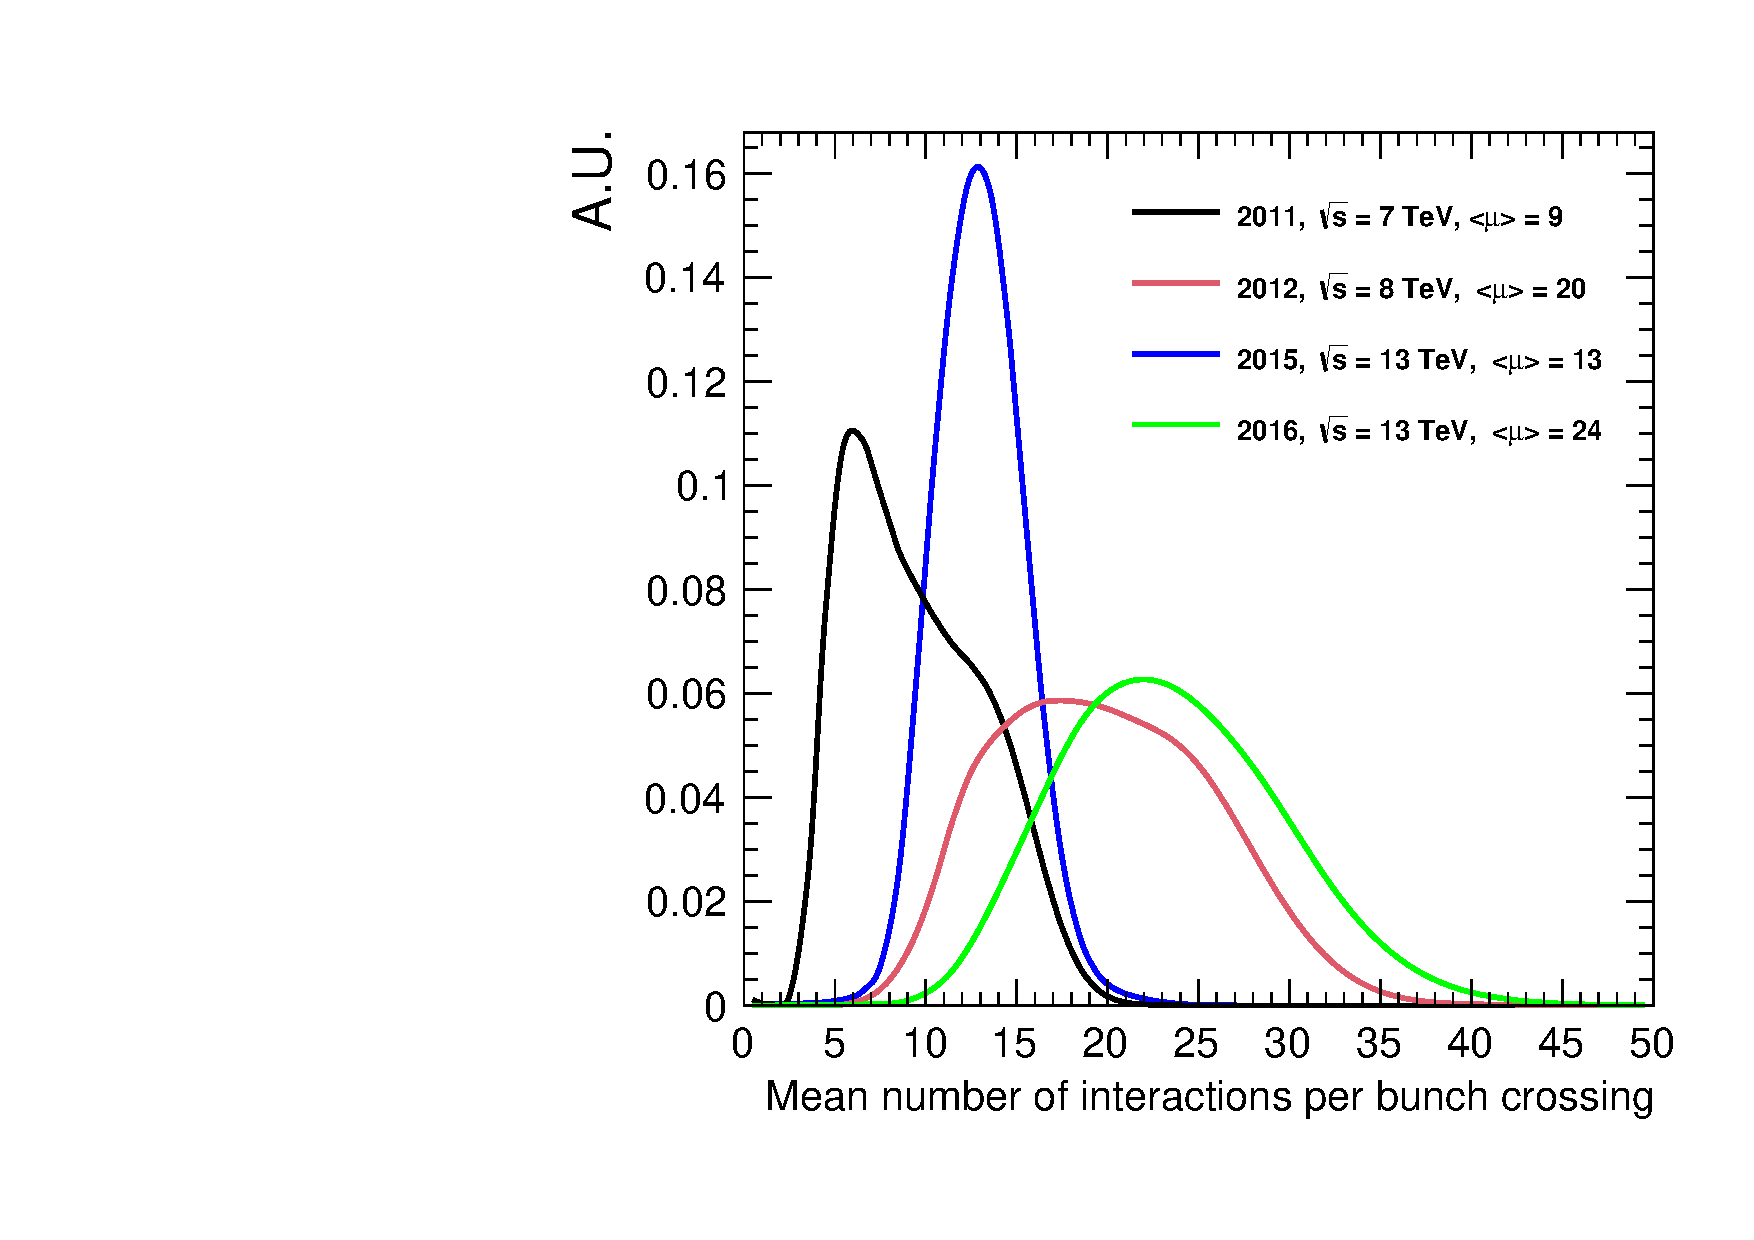
\includegraphics[width=0.6\columnwidth]{figures_chapter2/pileup_cms}
\caption{Mean number of interactions per bunch crossing in proton-proton collisions. A detailed description of the  luminosity measurements in CMS can be found here~\cite{CMS-PAS-LUM-13-001,CMS-PAS-LUM-15-001}. The distributions are shown for $2011$ (black), $2012$ (red), $2015$ (blue), and $2016$ (green) data taking periods.}
\label{fig:pu}
\end{figure} 

The LHC entered the Long Shutdown $1$ (LS1) in $2013$ for maintenance and upgrades during which the CMS detector was upgraded as well. The data taking resumed in $2015$ with $4.2~\ifb$ total integrated luminosity delivered to CMS with a peak instantaneous luminosity of $5.1 \times 10^{33}$ cm$^2$ s$^{-1}$. The LHC started to operate with the nominal bunch spacing of $25$ ns during this period. The total certified data for the nominal CMS operation and bunch spacing of $25$ ns amounted to $2.3~\ifb$. The data taking continued in $2016$ with an excellent performance by the LHC with significantly lower transverse beam sizes. This was achieved using a new bunch production scheme which resulted in a peak luminosity of  $1.2 \times 10^{34}$ cm$^2$ s$^{-1}$. Total integrated luminosity of $26.1~\ifb$ was delivered by the end of August of $2016$.   

Figure~\ref{fig:pu} shows the mean number of additional inelastic proton-proton interactions per bunch crossing (pileup). The additional pileup interactions in events present challenges in reconstruction and identification of the particles originating from the hard scattering of interest. The average number of pileup interactions in $2011$ was $9$ as the instantaneous luminosity continuously increased during the year. The average number of pileup interactions further increased to $20$ in $2012$ and reached to $24$ during $2016$.  While higher instantaneous luminosities are desired to enhance the production of the events of interest, the effects of pileup need to be mitigated to improve the sensitivity of the results. 

\section{Proton-Proton Collisions and Event Simulation}

The $W$, $Z$, and Higgs bosons are produce via the interactions of the quarks and gluons (referred as partons) inside the protons of the LHC colliding proton beams~\cite{Bloom:1969kc,Breidenbach:1969kd}. The cross section of a given process is given by:

\begin{figure}[!h]
\centering
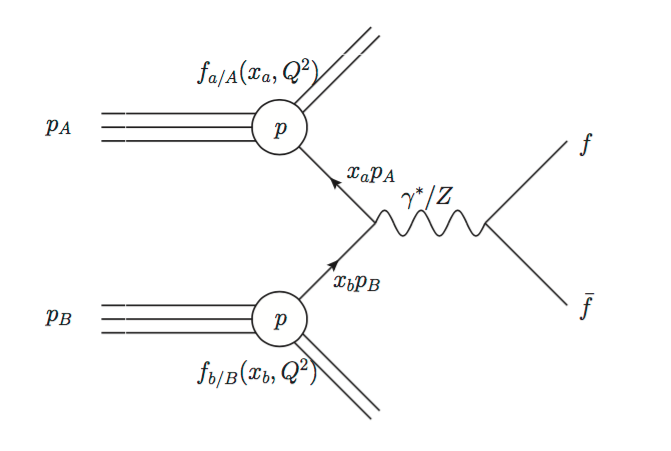
\includegraphics[width=0.60\columnwidth]{figures_chapter2/lhc_cross}
\caption{Illustration of the $Z$ boson production in proton-proton collisions. The parton momenta are given by $x_ap_a$ and $x_bp_b$~\cite{Schott:2014sea}.}
\label{fig:lhc_collision}
\end{figure} 

\begin{eqnarray} \label{eq:xsec}
\begin{aligned}
\sigma_{p_ap_b \rightarrow n} &= \sum_{a,b} \int dx_a dx_b f_{a/A}(x_a,\mu_{F}^2) f_{b/B}(x_{b},\mu_{F}^2)  \\ 
& \times [\hat{\sigma}_{LO}(x_ax_bs,\mu_R^2,\mu_F^2)+\alpha_s(\mu_R^2)\hat{\sigma}_{NLO}(x_ax_bs,\mu_R^2,\mu_F^2)+...],
\end{aligned}
\end{eqnarray}   
where $f(a/A)$, $f_{b/B}$ are the parton distribution functions (PDF) for the quarks and gluons inside the proton, $x_i$ is the relative parton momentum in the direction of proton, and $\hat{\sigma}$ denote the parton-parton cross section at the centre-of-mass energy $x_{a}x_{b}s$, where $s$ is the squared of the proton-proton centre-of-mass energy.  This is illustrated in Figure~\ref{fig:lhc_collision} for the $Z$ boson production. The PDFs can not be described through perturbative calculations however the collinear factorization theorem can be applied to separate the perturbative and non-perturbative regimes in Eq.~(\ref{eq:xsec})~\cite{Collins:1989gx}. The scale at which this separation happens is denoted as the factorization scale $\mu_{F}$. The basic idea is to absorb the large logarithms appearing in the calculations due to collinear emissions of the parton into the PDFs. This scale dependance of the PDFs is described by the Dokshitzer-Gribov-Lipatov-Altarelli-Parisi (DGLAP) parton evolution equations allowing to evolve a given PDF parametrization to a desired scale~\cite{Gribov:1972ri,Altarelli:1977zs,Dokshitzer:1977sg}. In this way a parameterized functional forms are fitted to data and then evolved to a scale of interest by solving the DGLAP equations either in leading-order, next-to-leading-order (NLO) or NNLO. PDF fits by several collaborations are used in the results.

The matrix elements (ME) needed to evaluate the partonic cross sections are performed using a Monte Carlo sampling to integrate the phase space. The QCD ME calculations are done up to a fixed number of final state partons. The transverse momenta of the bosons are zero at LO calculations. The real emissions in the higher order QCD corrections can explain the observed $p_{T}$ distributions of the $W$ and $Z$ bosons for example (there is also a very small boson $p_{T}$ due to a small transverse momentum of the parton inside proton). Thus measuring the $p_{T}$ distributions of these bosons provides new constraints to understand the higher order QCD (and electroweak) corrections. At small vector boson $p_{T}$ values large logarithmic corrections appear in fixed order calculations due to collinear gluon emissions. These logarithmic corrections due to these emissions cancel with the virtual corrections for the inclusive calculations. Resummation can be carried out to provide accurate predictions of the vector boson $p_{T}$ at the low values of the $p_T$~\cite{Laenen:1991af}.

ME calculations at fixed orders break down for soft momenta and collinear final state partons. Parton shower models are used to evolve the partons from the hard scales to the non-perturbative hadron scales. The parton showers are modeled as a sequence os branchings $q \rightarrow qg$, $g \rightarrow q\bar{q}$, and $g \rightarrow g g$ in QCD and $q \rightarrow q\gamma$ and $\ell \rightarrow \ell \gamma$ in quantum eletrodynamics (QED) where $q$, $g$, $\ell$, and $\gamma$ denote a quark, gluon, lepton, and photon respectively~\cite{Schott:2014sea}. The branchings from the initial and final partons add additional outgoing partons in the event. It has to be noted that unlike the ME approach the parton method does not include the spin effects. 

The parton showering is continued up to the scale $\Lambda_{QCD} \approx 200~\MeV$. The final partons are hadronized into color-neutral hadrons to obtain the full generated event simulation. The models are tuned to the data. The unstable hadrons (traveling less than few mm) are decayed according to the branching ratios. Additional parton-parton interactions in the colliding protons, known as multi-parton interactions (MPI), are included as well. The specific software tools utilized to generate the events used in the results are referenced in chapter $4$.  

\section{The $W$,$Z$, and Higgs boson productions at the LHC}

The production of the electroweak gauge bosons at the LHC proton-proton collisions is mainly via the Drell-Yan process~\cite{Drell:1970wh}. At least one sea quark is required to produce the gauge bosons in the proton-proton collisions and it is dominated by $u\bar{d} \rightarrow W^{+}$, $d\bar{u} \rightarrow W^{-}$, and $u\bar{u},d\bar{d} \rightarrow Z$. The relations between the mass $M$ and rapidity $y$ of the vector boson and the kinematics of the colliding partons are given by:
\begin{eqnarray} \label{eq:kinematics}
\begin{aligned}
M^2 &= x_{1}x_{2}s, \\
y &= \frac{1}{2} \mathrm{ln}\left(\frac{E+p_{z}}{E-p_{z}}\right) = \frac{1}{2}\mathrm{ln}\left(\frac{x_1}{x_2}\right), \\
x_{1/2} &= \frac{M}{\sqrt{s}} \mathrm{exp}(\pm y).
\end{aligned}
\end{eqnarray}   

\begin{figure}[!h]
\centering
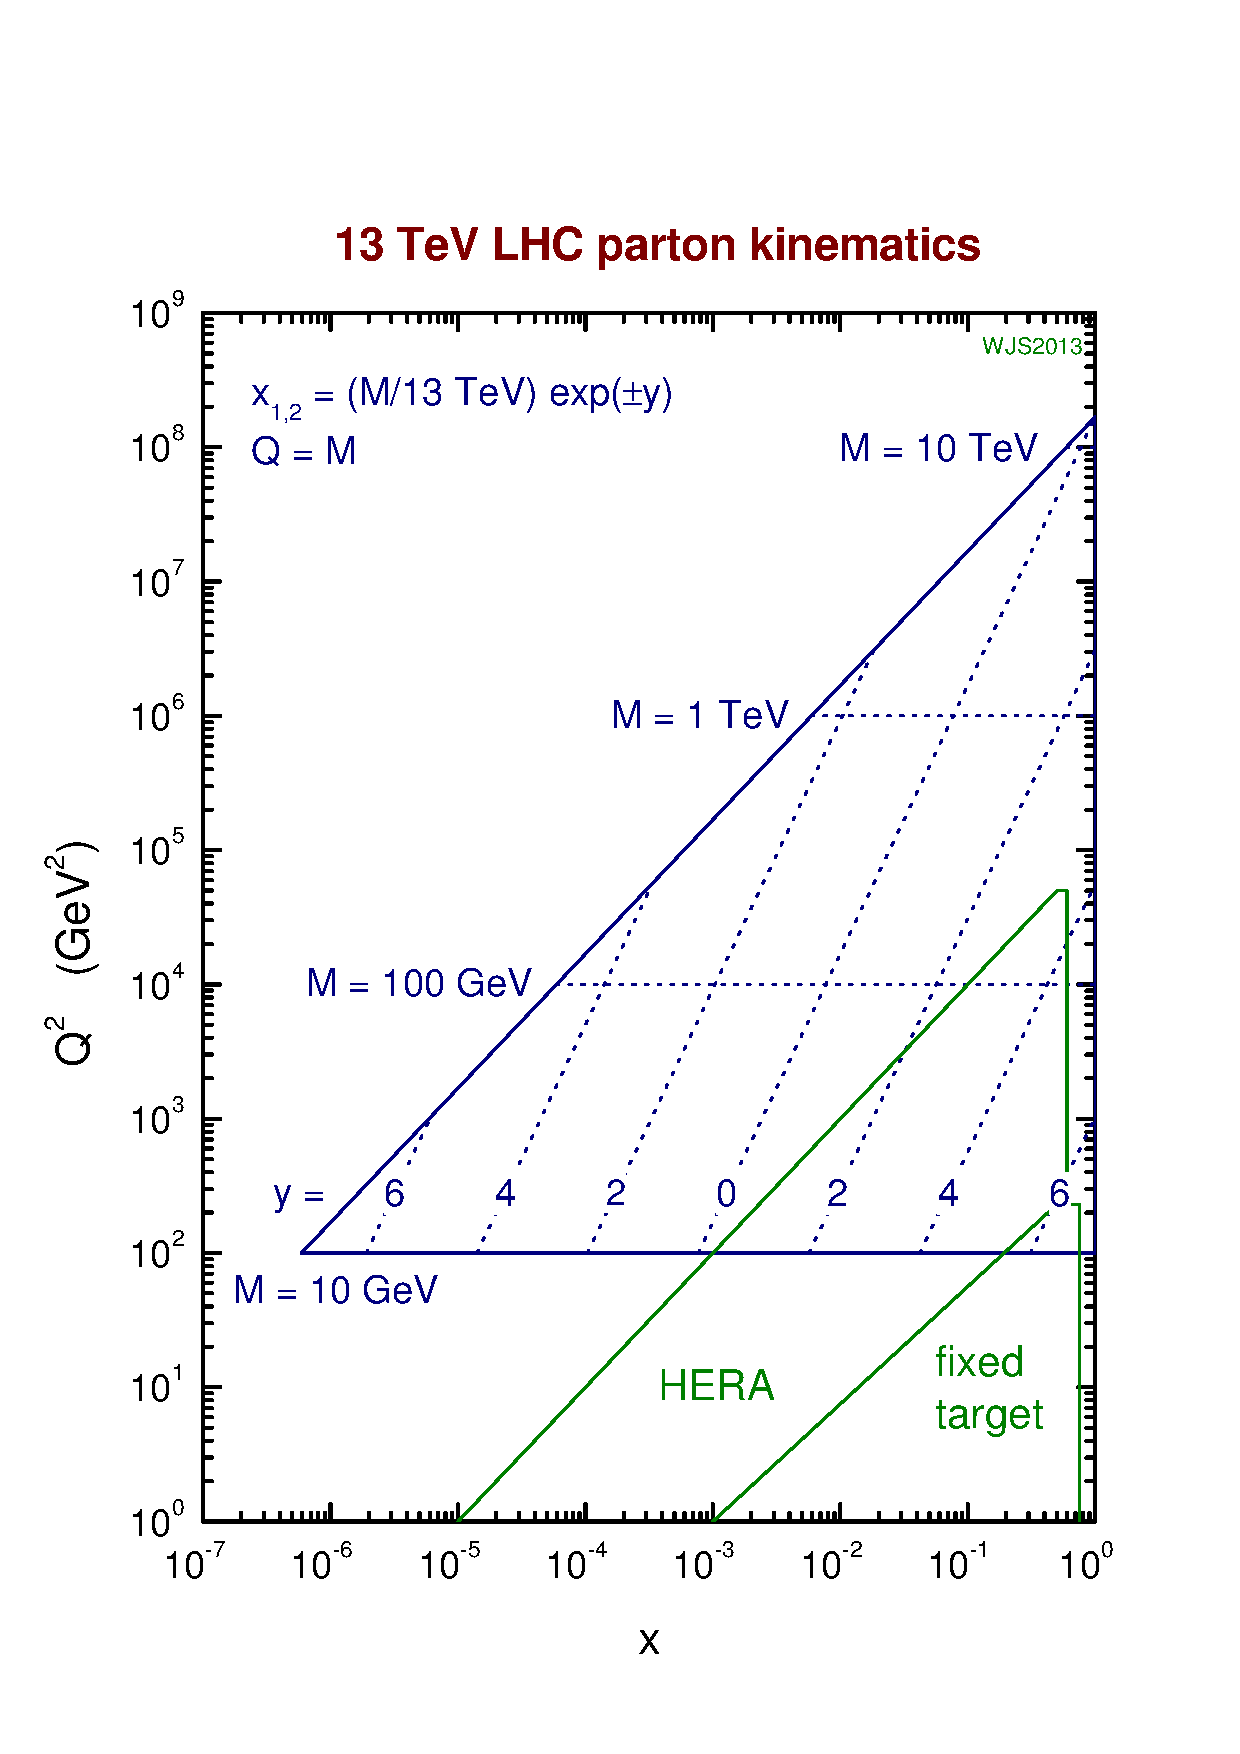
\includegraphics[width=0.49\columnwidth]{figures_chapter2/lhcgrid13}
\caption{Available kinematic plane in Bjorken-$x$ and the scale of the process $Q^2$ at the LHC centre-of-mass energy $\sqrt{s}=13~\TeV$. $M$ and $y$ are the mass and rapidity of the final state parton. The corresponding plane for the deep inelastic experiments is shown in green~\cite{sterling}. }
\label{fig:lhc_grid}
\end{figure} 

This is illustrated in Figure~\ref{lhc_grid}. Hence for the $W$ and $Z$ boson production with masses of $\mathcal{O} (100~\GeV)$ and rapidity $|y|<2.5$ the Bjorken-$x$ values are in the range of $10^{-3}$ to $0.1$. Theoretical predictions of the inclusive $W$ and $Z$ production cross sections are available at NNLO in perturbative QCD~\cite{Rijken:1994sh,Hamberg:1990np,vanNeerven:1991gh,Harlander:2002wh,PhysRevD.69.094008}. The precision of the predictions is limited by the uncertainties in PDFs and higher order QCD and EWK corrections. The energy scale of the process means that the sea quarks in the protons are mainly due to the gluon splitting $g \rightarrow q\bar{q}$ and therefore the uncertainty of the gluon PDFs plays a role as well.

The leptonic decays of the $W$ and $Z$ bosons provide a large dataset of relatively pure and isolated leptonic events. $Z \rightarrow \ell \ell$ events can be used to calibrate the detector as well as the luminosity stability of the proton-proton collisions. The inclusive total cross section measurements and ratios test the perturbative higher order corrections and constrain the PDFs of the protons. The importance of the higher order QCD corrections on the boson transverse momenta distribution was discussed in the last section. The better understanding of these effects allows to make precise measurements of the fundamental electroweak parameters such as the mass of the $W$ boson and the electroweak mixing angle. In addition the $W$ and $Z$ boson production is a background source for the SM Higgs boson studies and many BSM physics searches.


\begin{figure}[!h]
\centering
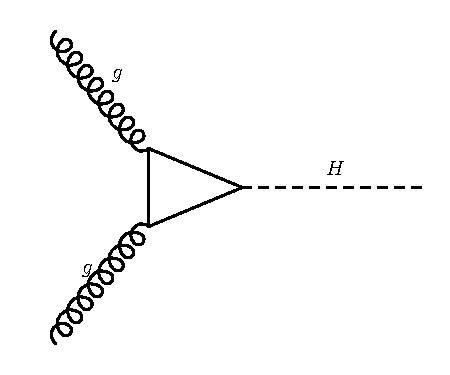
\includegraphics[width=0.49\columnwidth]{figures_chapter2/g_fusion}
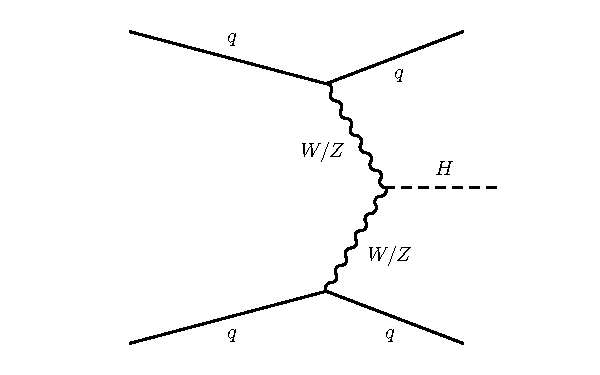
\includegraphics[width=0.49\columnwidth]{figures_chapter2/vbf}
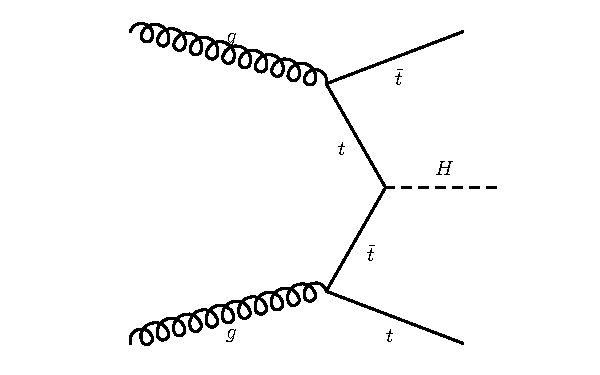
\includegraphics[width=0.49\columnwidth]{figures_chapter2/tth}
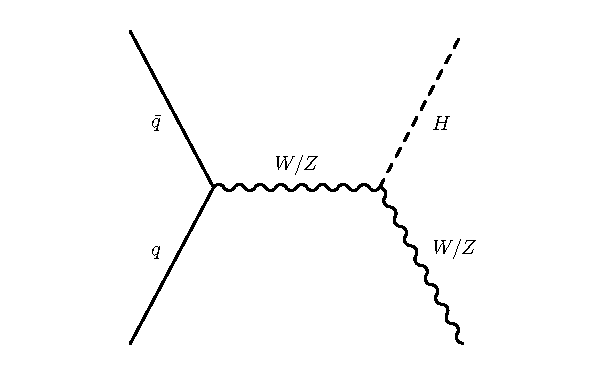
\includegraphics[width=0.49\columnwidth]{figures_chapter2/vh}
\caption{Leading order Feynman diagrams contributing to Higgs boson production at the LHC in gluon fusion (top left), vector boson fusion (top right), Higgsstrahlung (bottom left), and top quark associated production (bottom right). }
\label{fig:sm_higgs}
\end{figure} 


Figure~\ref{fig:sm_higgs} shows the main leading order Ferynman diagrams contributing to the SM Higgs boson production at the LHC. The gluon fusion production, where the Higgs is produced from an intermediate quark loop, is the dominant mode~\cite{Georgi:1977gs}. It is dominated by the top quark loop as the Higgs coupling to fermions is proportional to the mass of the fermion in question. The Vector Boson Fusion (VBF) production~\cite{Cahn:1983ip}, where the Higgs boson is produced from an intermediate $W/Z$ bosons radiated from the colliding quarks has an interesting experimental signature that can be exploited.  The VBF produced Higgs events are produced in association with two high energy forward jets (the jets are discussed in chapter $3$) in the opposite regions of the detector.  There is typically very little hadronic activity in the central region of the detector as there is no "color flow" between the quarks. Higgsstrahlung~\cite{Glashow:1978ab}, where the Higgs boson is radiated from a $W$ or $Z$ boson produced in $s$ channel at leading order, is the next largest Higgs boson production mode.  The Higgs bosons produced in VBF and Higgsstrahlung processes tend to have higher transverse momentum compared to Higgs bosons produced in the gluon fusion mode. The Higgs boson can also be produced in association with a top and anti-top pair~\cite{Raitio:1978pt,Ng:1983jm.Kunszt:1984ri,Marciano:1991qq}.There are other Higgs production modes, not relevant for the current Higgs boson studies, that will be important to consider at higher integrated luminosities at the LHC. The SM Higgs boson production cross sections are shown in Figure~\ref{fig:higgs_cross} as a function of the Higgs boson mass at $\sqrt{s}=8~\TeV$ and as a function of $\sqrt{s}$ for the Higgs mass of $125~\GeV$. The individual cross sections for the four Higss boson production mechanisms discussed above are shown. The calculations are done up to NNLO in QCD and NLO in EWK~\cite{Dittmaier:2011ti,Dittmaier:2012vm,Heinemeyer:2013tqa}. The gluon fusion predictions are also resummed to NNLL accuracy. Recent calculations to $N^{3}LO$ in QCD for the gluon fusion~\cite{Anastasiou:2016cez} and VBF production modes~\cite{Dreyer:2016oyx} have become available.

\begin{figure}[ht]
\centering
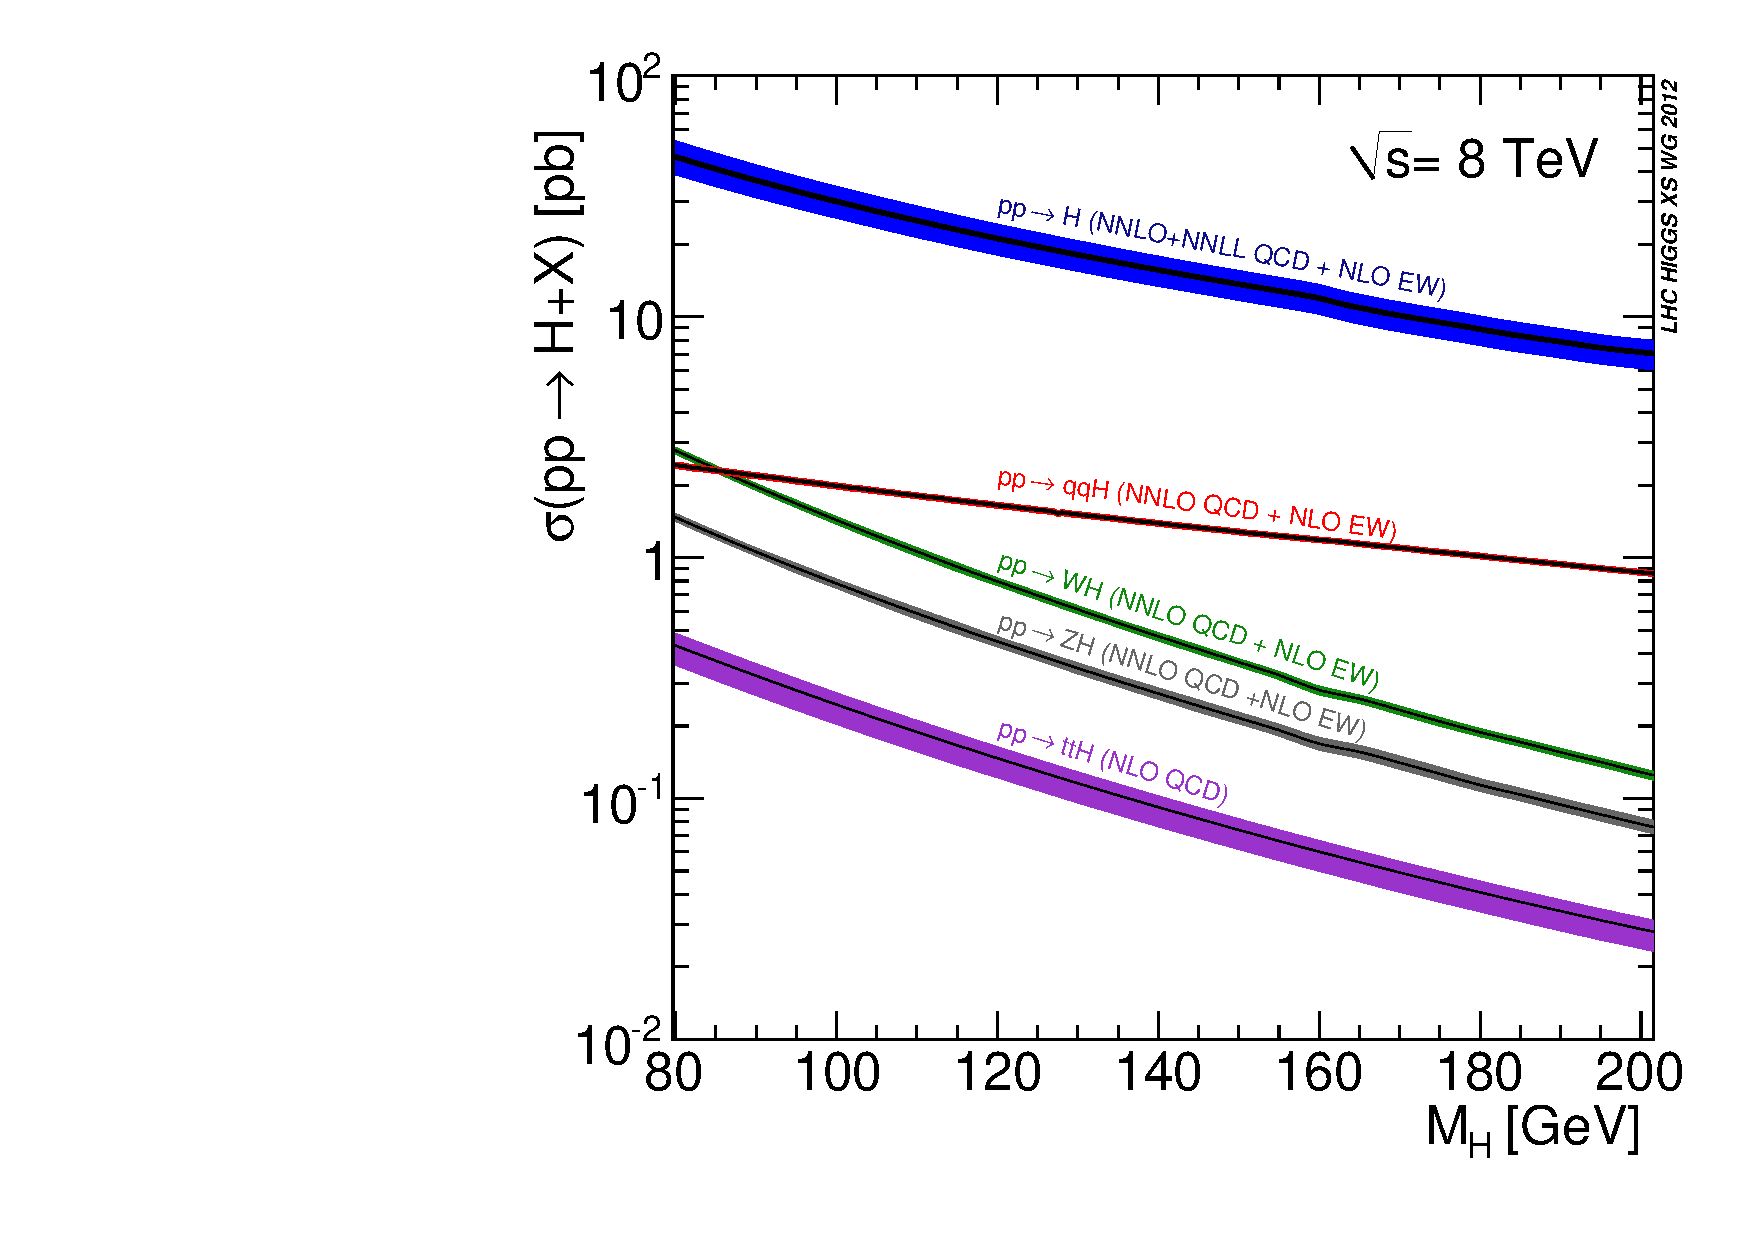
\includegraphics[width=0.49\columnwidth]{figures_chapter2/Higgs_XS_8TeV_LM200}
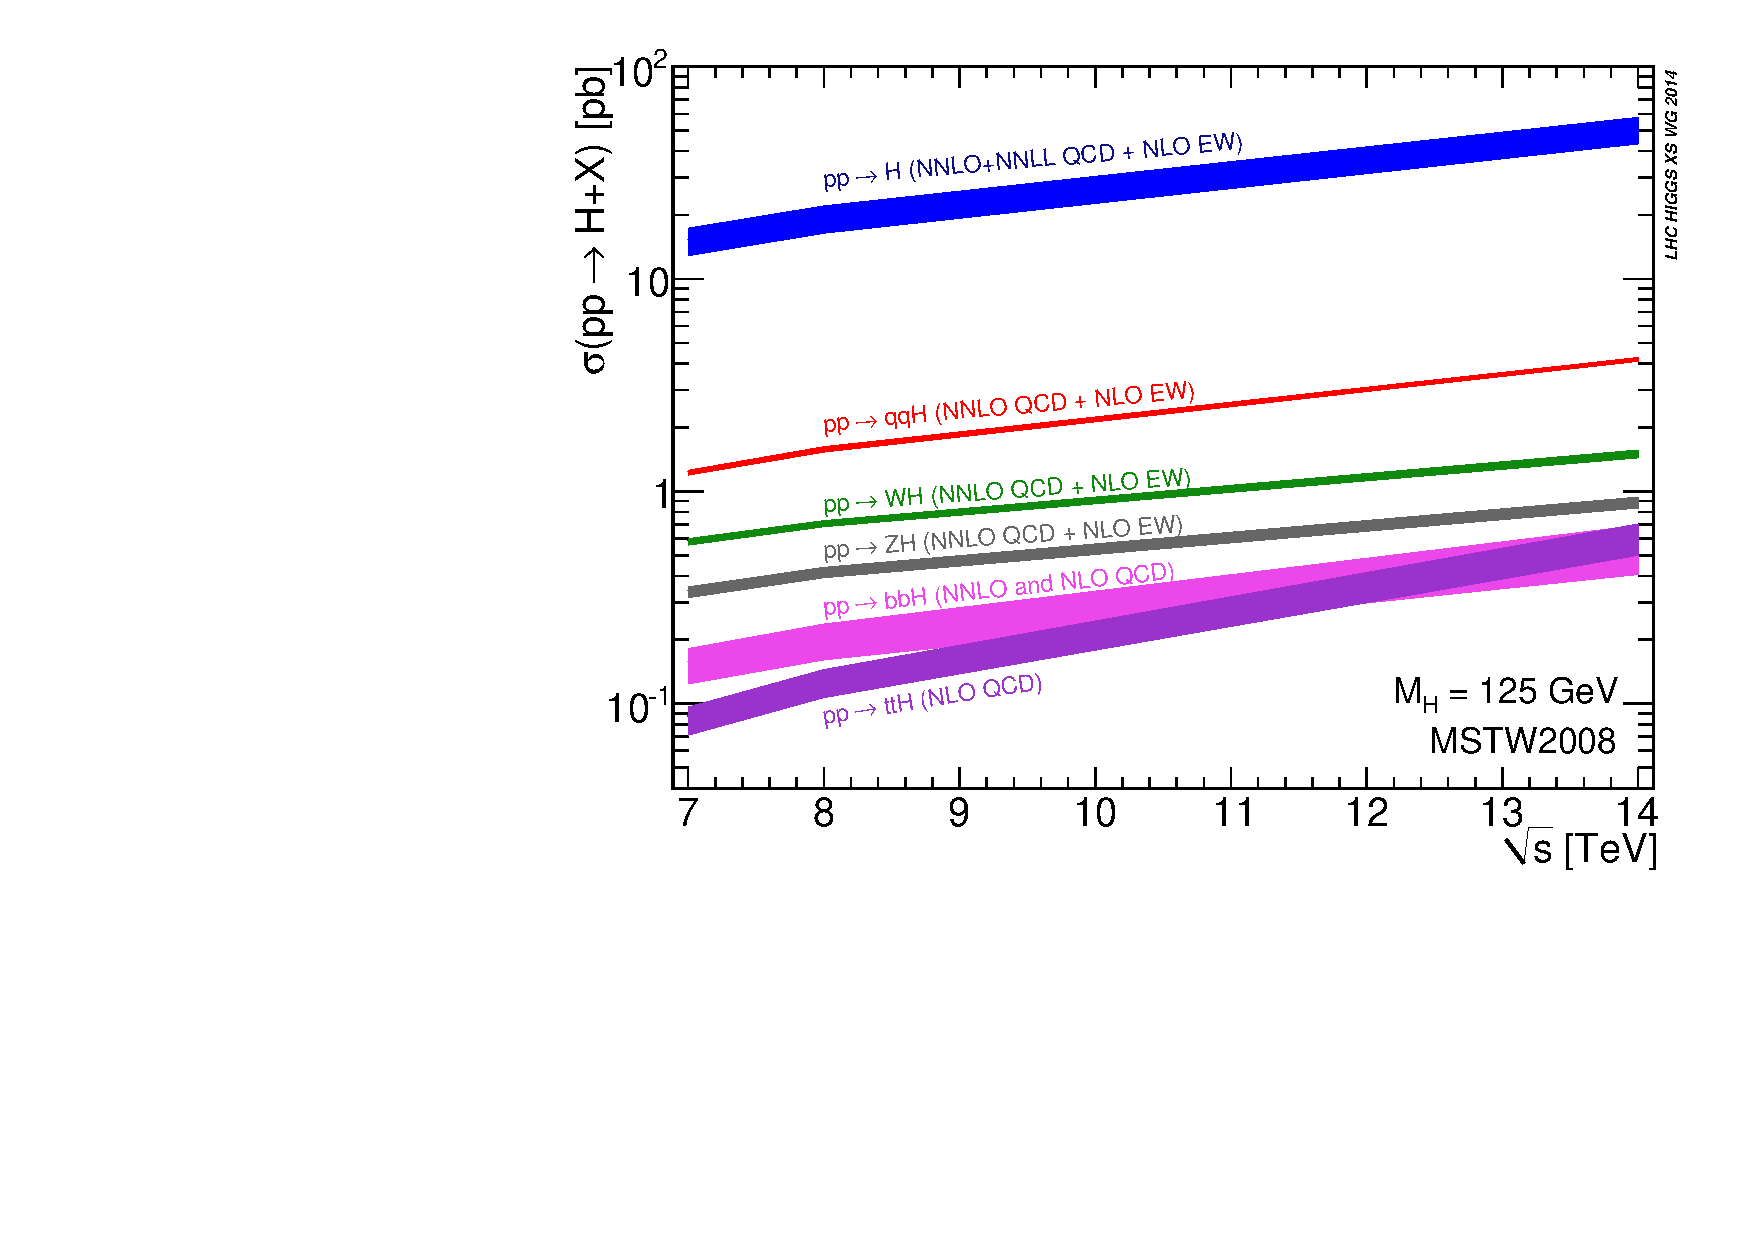
\includegraphics[width=0.49\columnwidth]{figures_chapter2/7-14}
\caption{Higgs boson production cross sections for the different production modes as a function of the Higgs mass at $\sqrt{s}=8~\TeV$ (left panel) and centre-of-mass energy $\sqrt{s}$ for the Higgs mass of $125~\GeV$ (right panel)~\cite{Dittmaier:2011ti,Dittmaier:2012vm,Heinemeyer:2013tqa}.}
\label{fig:higgs_cross}
\end{figure} 

The branching 

\begin{figure}[!h]
\centering
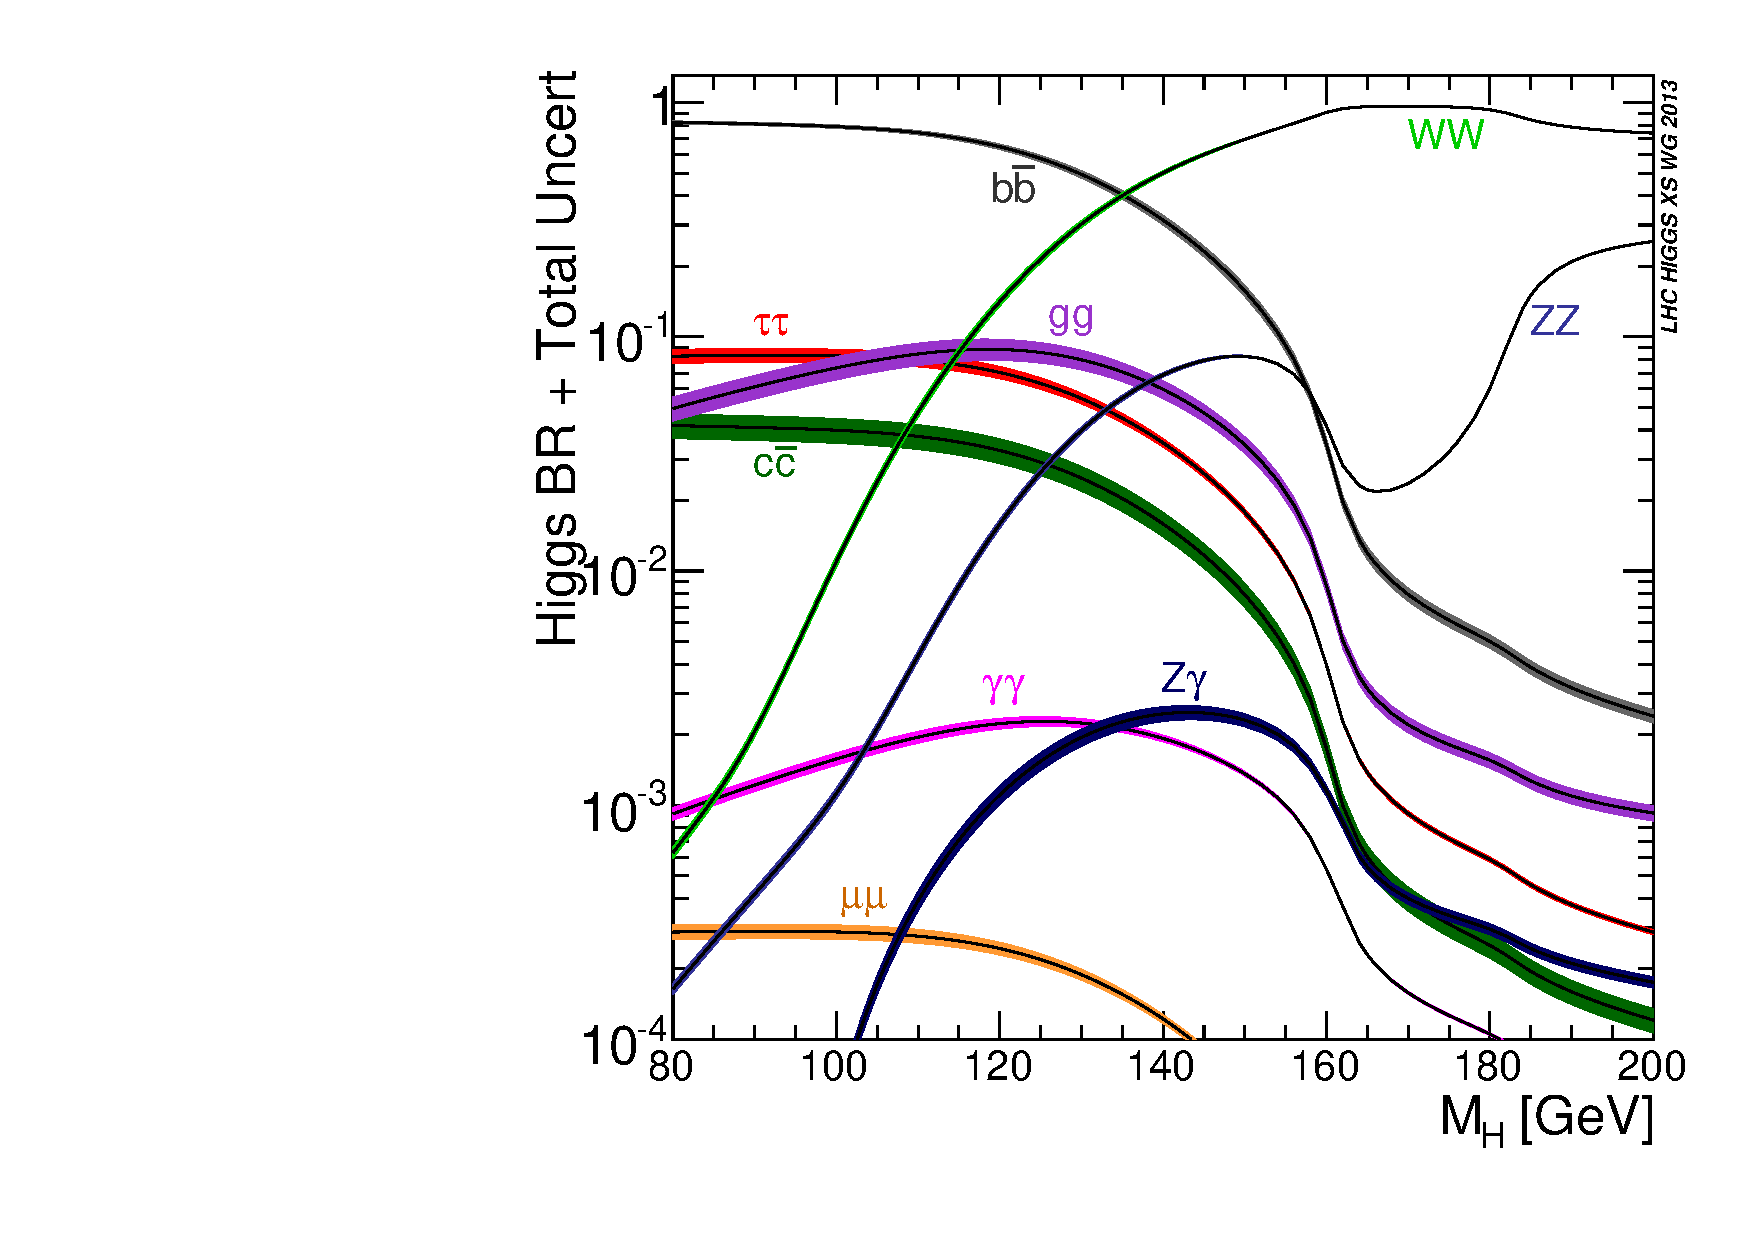
\includegraphics[width=0.49\columnwidth]{figures_chapter2/Higgs_BR_LM}
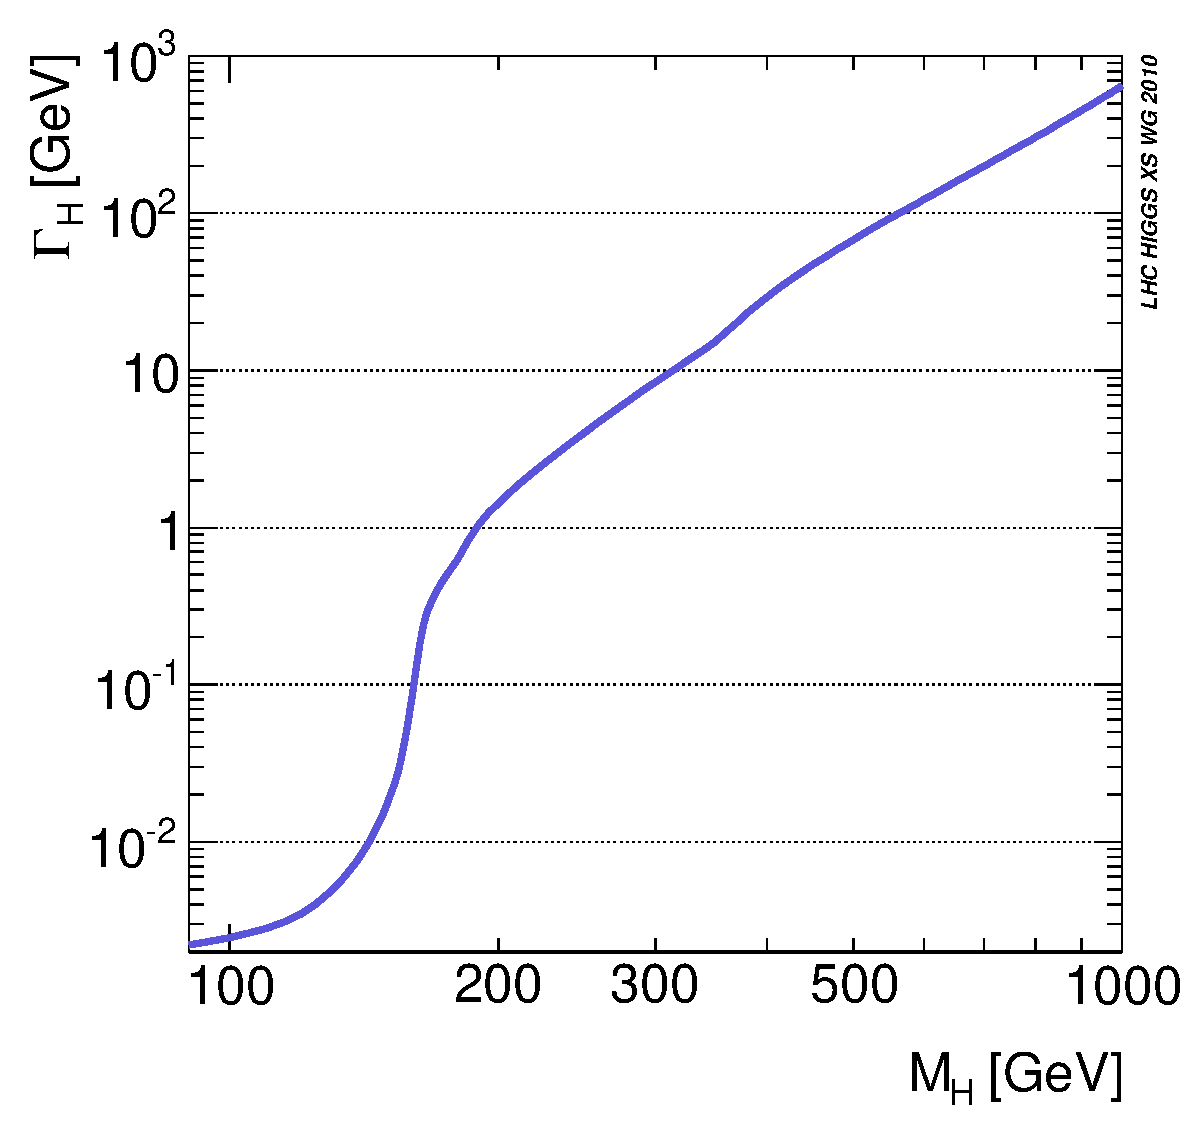
\includegraphics[width=0.49\columnwidth]{figures_chapter2/YRHXS_BR_fig2}
\caption{The largest Higgs boson branching ratios as a function (left panel) and total width as a function of the Higgs mass.~\cite{Dittmaier:2011ti,Dittmaier:2012vm,Heinemeyer:2013tqa}.} 
\label{fig:higgs_decay}
\end{figure} 

The SM Higgs boson pair production to be discussed.

\begin{figure}[!h]
\centering
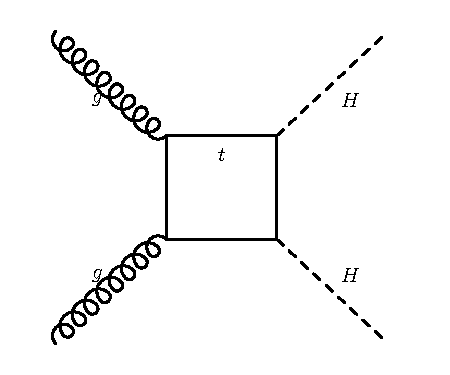
\includegraphics[width=0.49\columnwidth]{figures_chapter2/hhbox}
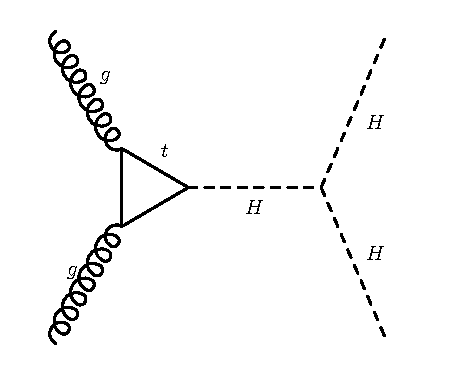
\includegraphics[width=0.49\columnwidth]{figures_chapter2/hhself}
\caption{Leading order Feynman diagrams contributing to the gluon fusion Higgs boson pair production at the LHC. The right diagram is the Higgs boson self-coupling contribution to the Higgs pair production.}
\label{fig:sm_dihiggs}
\end{figure} 

The MSSM Higgs boson production to be discussed.

\begin{figure}[!h]
\centering
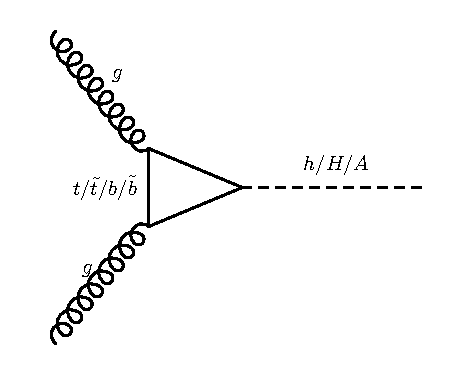
\includegraphics[width=0.49\columnwidth]{figures_chapter2/mssm_fusion}
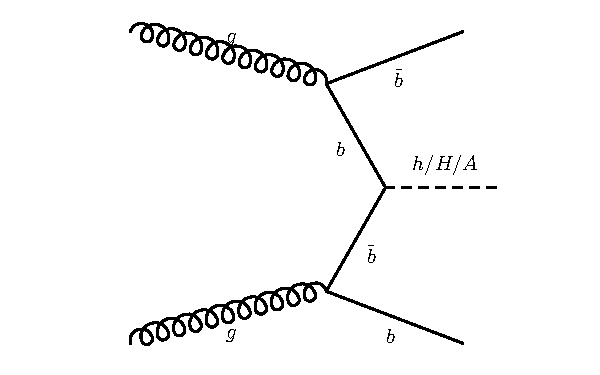
\includegraphics[width=0.49\columnwidth]{figures_chapter2/bbh_mssm}
\caption{Leading order Feynman diagrams contributing to the production of the MSSM Higgs bosons in gluon fusion (left) and b quark associated production (right).}
\label{fig:mssm_feynman}
\end{figure} 

\begin{figure}[!h]
\centering
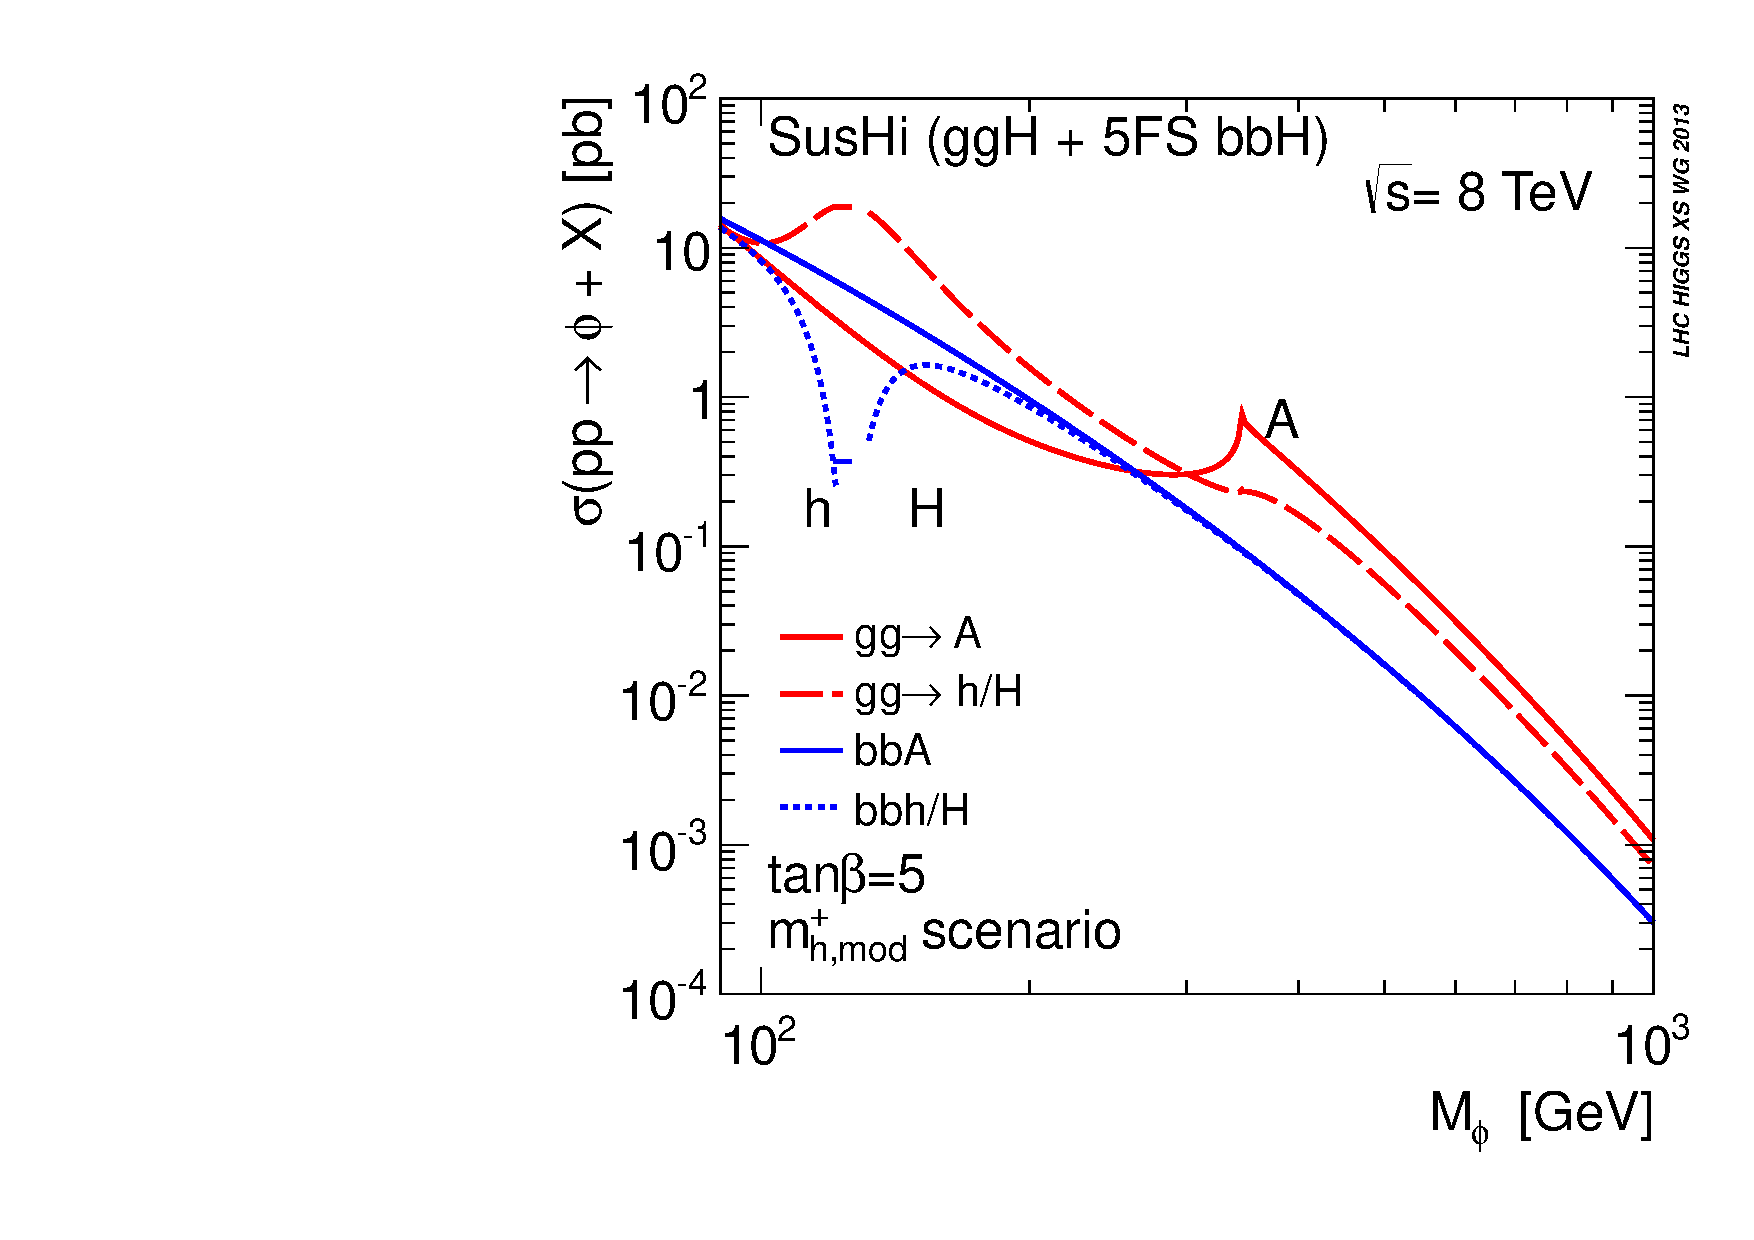
\includegraphics[width=0.49\columnwidth]{figures_chapter2/YR3HXS_XSectSummary_mhmodp_tanbeta5_SusHi}
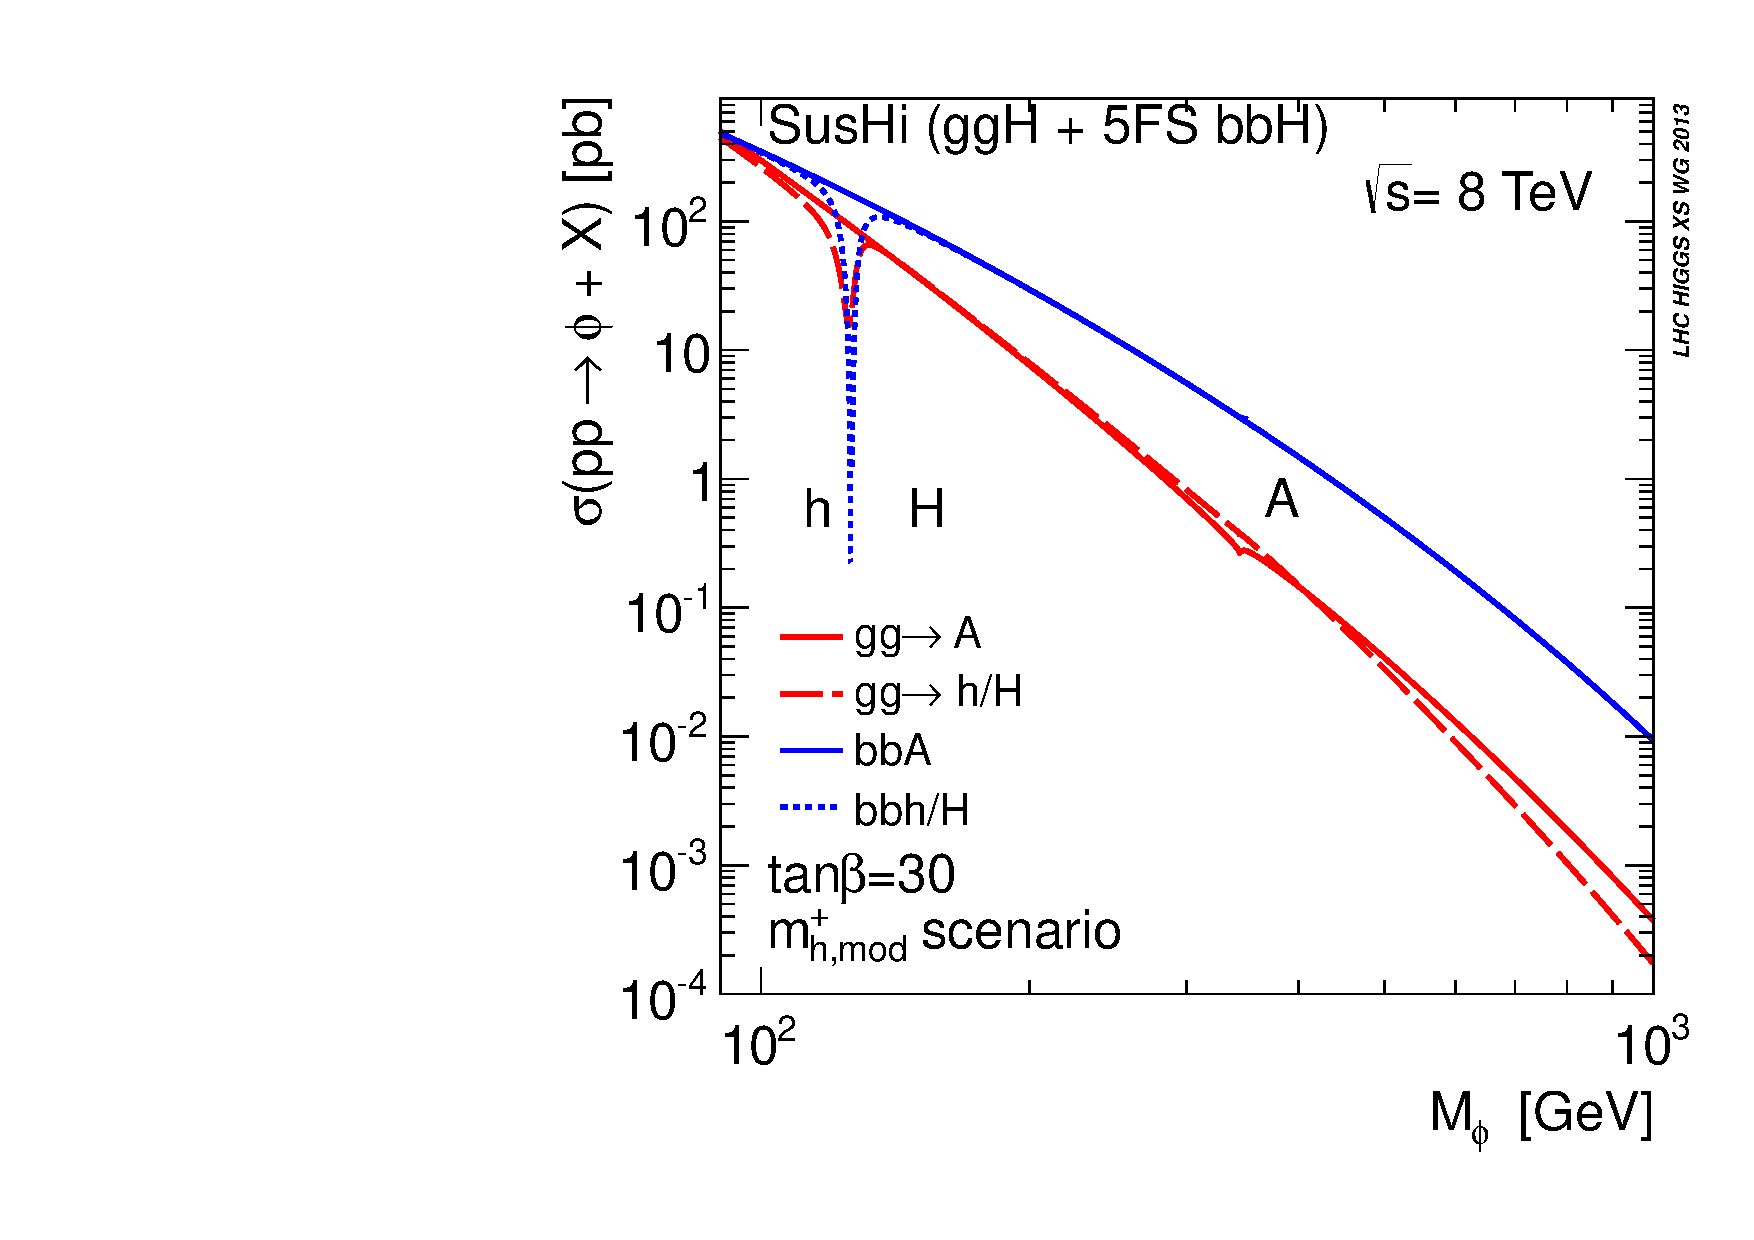
\includegraphics[width=0.49\columnwidth]{figures_chapter2/YR3HXS_XSectSummary_mhmodp_tanbeta30_SusHi}
\caption{Neutral Higgs boson production cross sections as a function of the CP-odd Higgs mass in the $m_{h}^{mod+}$ benchmark scenario with $\tan \beta = 5$ (left panel) and $\tan \beta = 30$ (right panel)~\cite{Dittmaier:2011ti,Dittmaier:2012vm,Heinemeyer:2013tqa}.} 
\label{fig:mssm_cross}
\end{figure} 

\begin{figure}[!h]
\centering
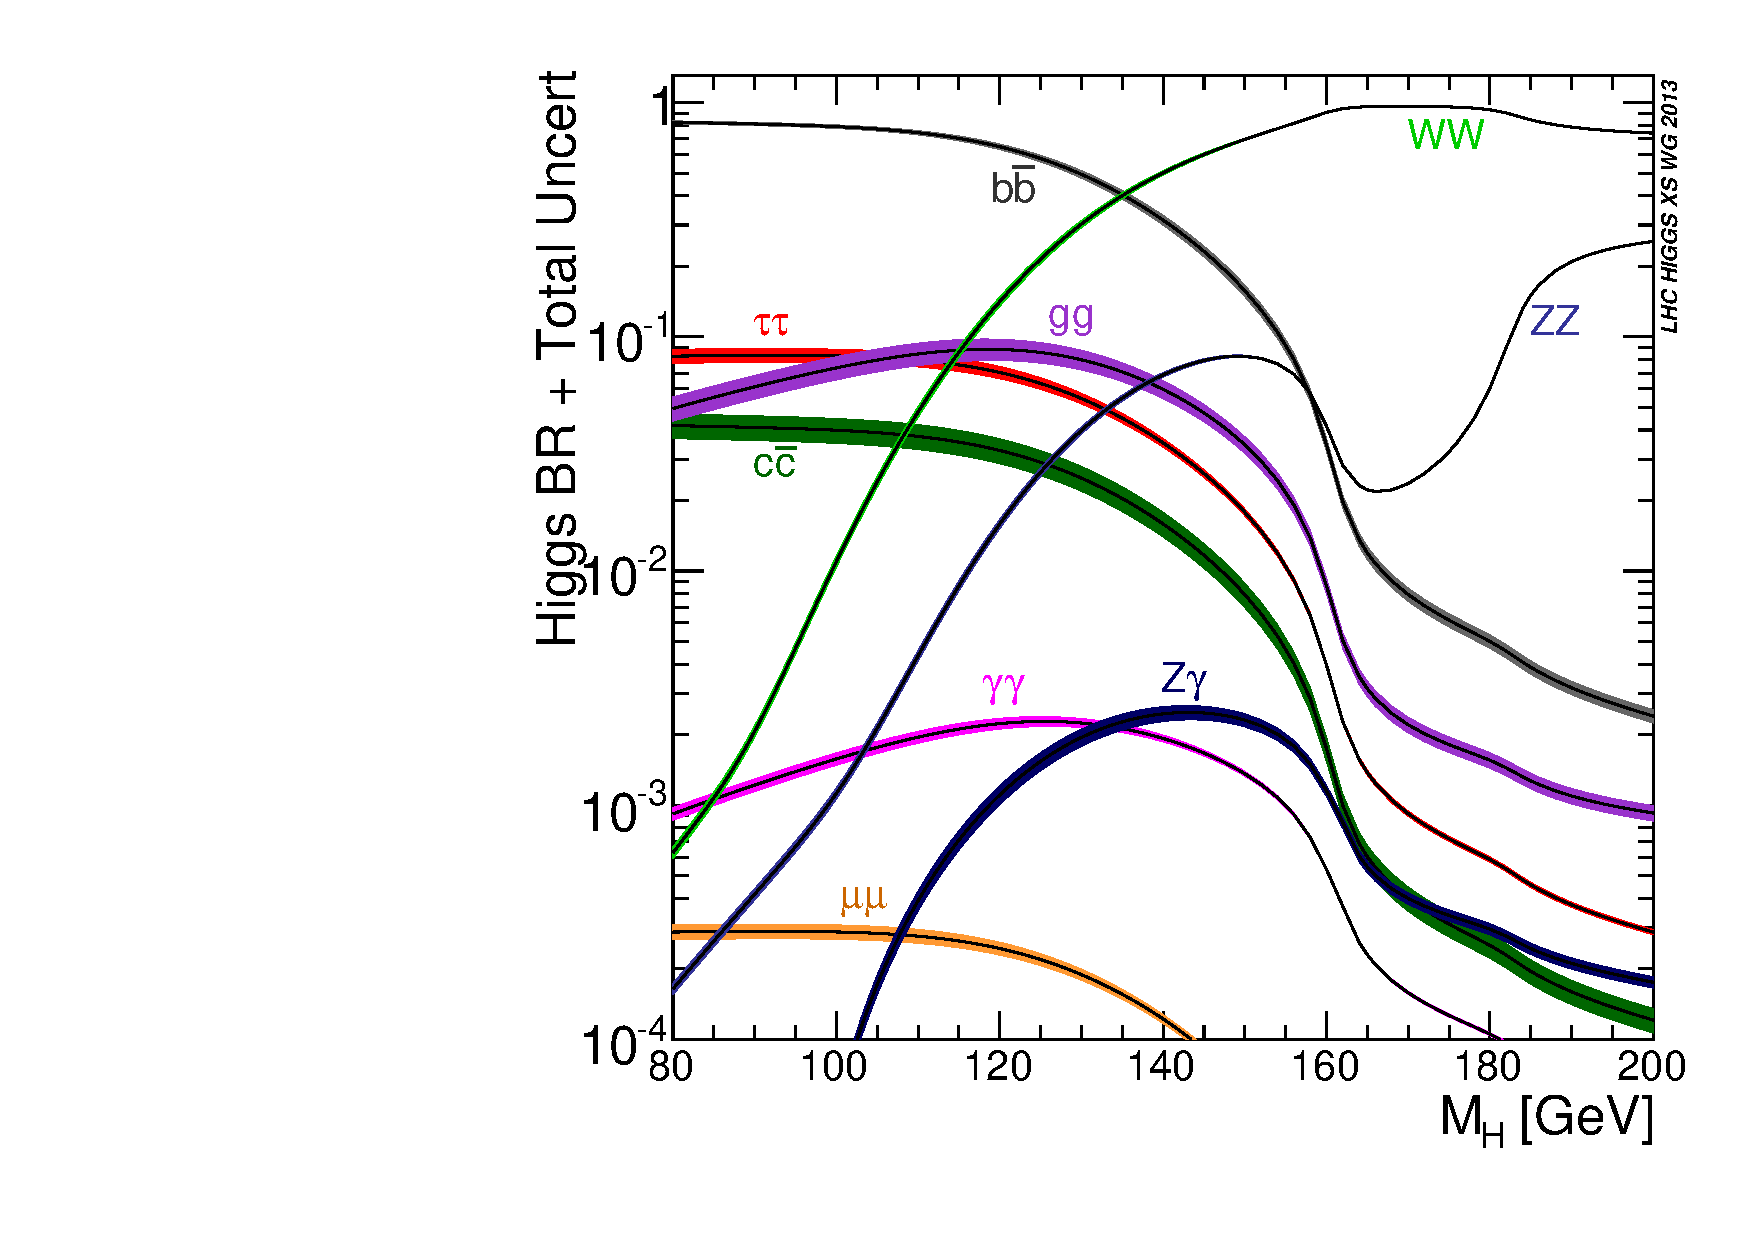
\includegraphics[width=0.49\columnwidth]{figures_chapter2/Higgs_BR_LM}
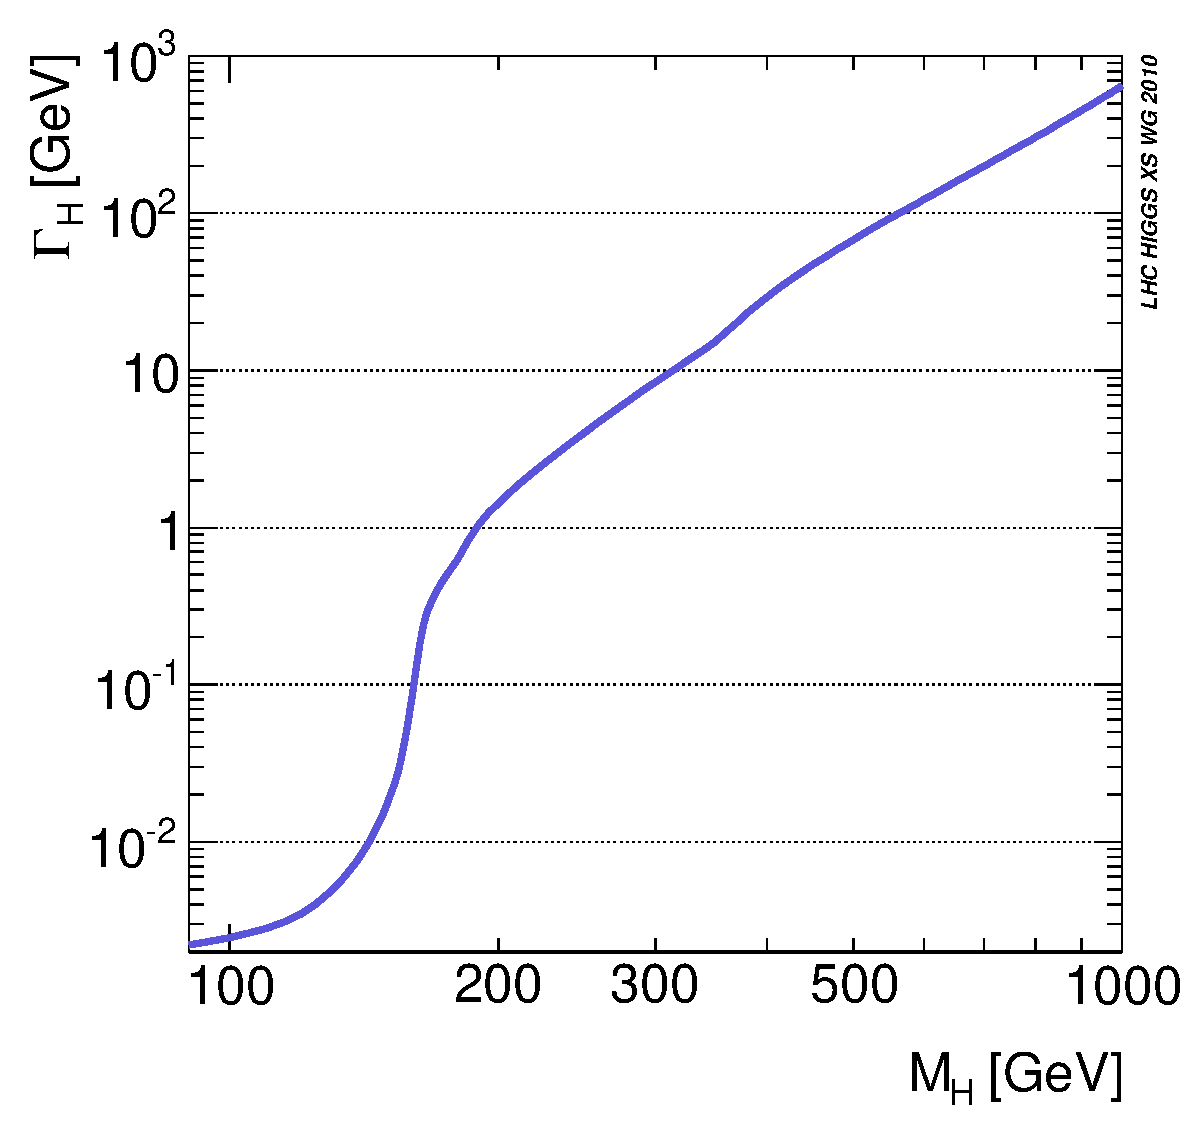
\includegraphics[width=0.49\columnwidth]{figures_chapter2/YRHXS_BR_fig2}
\caption{Neutral CP-odd Higgs boson branching fractions as a function of the mass in the $m_{h}^{mod+}$ benchmark scenario with $\tan \beta = 5$ (left panel) and $\tan \beta = 30$ (right panel)~\cite{Dittmaier:2011ti,Dittmaier:2012vm,Heinemeyer:2013tqa}} 
\label{fig:mssm_decay}
\end{figure} 








%% This is an example first chapter.  You should put chapter/appendix that you
%% write into a separate file, and add a line \include{yourfilename} to
%% main.tex, where `yourfilename.tex' is the name of the chapter/appendix file.
%% You can process specific files by typing their names in at the 
%% \files=
%% prompt when you run the file main.tex through LaTeX.
\chapter{The CMS experiment}
The major goal of the CMS detector\cite{Chatrchyan:2008aa} is to elucidate the EWSB through the discovery of the Higgs boson. However CMS is a general purpose detector enabling to perform precision SM measurements as well BSM physics searches at the $\TeV$ scale. The detector requirements, driven by the physics program, include good reconstruction and momentum resolution of charged particles, good electromagnetic energy resolution, as well as good di-jet mass and missing energy resolutions. The large number of charged particles per interactions and the additional pileup interactions require a high granularity detector to be able to reconstruct all the individual charged particles.  Furthermore, a bunch spacing of $25$ ns requires a detector with good time resolution to be able to resolve the individual bunch crossings.  

The overall layout of the CMS detector is shown in Figure~\ref{fig:cms}. The detector is composed of several sub-detector layers with a length of $22$ m and a diameter of $15$ m. It has a cylindrical geometry with concentric barrel shaped detectors in the central region and disc shaped detectors in the forward region. The main feature of the CMS detector is a $3.8$ Tesla superconducting solenoid magnet that provides a large bending power to the charged particles. The length of the solenoid is $13$ m and the inner diameter is $6$ m. The inner tracking detectors, electromagnetic, and hadron calorimeters are located inside the solenoid. The muon detectors are embedded in the steel flux-return yoke of the magnet providing a sufficient magnetic field for a large bending power of the muons inside the muon detectors. The total weight of the CMS detector is $12500$ tonnes.  

\begin{figure}[h]
\centering
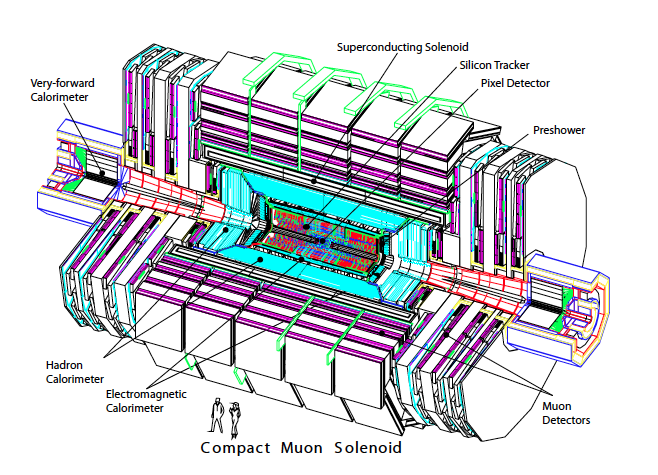
\includegraphics[width=1.0\columnwidth]{figures_chapter3/cms_detector}
\caption{A cutaway diagram of the CMS detector. The labels identify the different sub-detectors and the solenoid.}
\label{fig:cms}
\end{figure}

CMS uses the right-handed coordinate system. The origin is centered at the nominal collision point, x-axis is in the horizontal plane pointing towards the centre of the LHC tunnel, y-axis points vertically upwards, and the z-axis points along the beam direction toward the Jura mountains. It is convenient to employ the spherical coordinate system. The polar angle  $\theta$ is measured with respect to the positive z-axis and the azimuthal angle $\phi$ is measured from the positive x-axis in the x-y coordinate plane. The pseudorapidity is defined as $\eta = -\ln \tan(\frac{\theta}{2})$.  A useful consequence of this definition is that the difference between the pseudorapidities of two particles is Lorentz invariant with respect to a boost in the beam direction. The separation of two particles is defined by $\Delta R =\sqrt(\Delta \phi^2 + \Delta \eta^2)$. The momentum and energy transverse to the beam direction are denoted $p_{T}$ and $E_{T}$ respectively. The imbalance of the measured transverse energy is defined as a missing energy and denoted by $E_{T}^{miss}$.     

\section{Inner tracking detectors}

The inner tracking system\cite{Karim�ki:368412,addendum} surrounds the interaction point and has a length of $5.8$ m and a diameter of $2.5$ m. The goal of the inner tracking system is to make a precise and efficient measurement of the trajectories of charged particles as well as their momentum. In addition a precise reconstruction of secondary vertices is needed for the identification of heavy flavor particle decays. Tau lepton decays are identified by looking for one-prong and three-prong topologies in the inner tracker. A homogenous magnetic field of $3.8$ Tesla over the full volume of the tracker is provided by the CMS solenoid. 

There are $\mathcal{O}(1000)$ particles emerging from the interaction region at the nominal LHC luminosity for every $25$ ns bunch crossing. Therefore a high granular, fast, and radiation hard detector is required. On the other hand this implies a large power density of electronics and the corresponding cabling and cooling systems which increases the amount of material thereby enhancing the multiple scattering, photon conversions, and bremsstrahlung.    Silicon technology was chosen given the above considerations. Figure~\ref{fig:tracker} shows a schematic view of the inner tracking system in $r-z$ plane. The inner tracking detector covers a pseudorapidity range of up to $|\eta|=2.5$ and provides an average of $13-17$ measurements per charged particle depending on the $\eta$ region.

\begin{figure}[h]
\centering
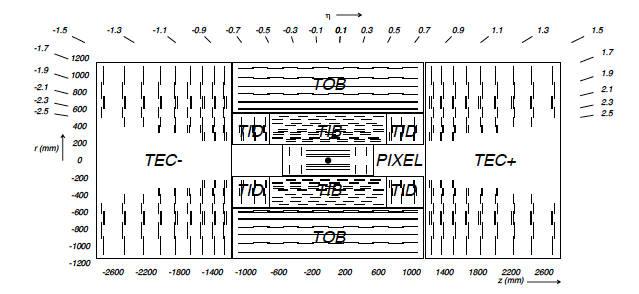
\includegraphics[width=1.0\columnwidth]{figures_chapter3/tracker_layout}
\caption{A schematic view of the CMS tracking system. Silicon pixel and strip detectors are shown. The double lines show back-to-back modules that deliver stereo hits.}
\label{fig:tracker}
\end{figure}

A pixelated detector has to be used close to the interaction region to keep the occupancy levels to less than $1\%$. The tracking system consists of three barrel layers and two endcap disks. The barrel layers are located at radii of $4.4$, $7.3$, and $10.2$ cm with a length of $53$ cm. The endcap pixel layers are located at $z=\pm 34.5$ and $z=\pm46.5$ cm covering approximately $6$ to $15$ cm in the radial direction. The pixel detector consists of $66$ million pixel elements covering a surface area of approximately of $1$ m$^2$. The pixel element size is $100\times150$ $\mu$m$^2$ providing a similar track resolution in both $r-\phi$ and $r-z$ directions. Each pixel is a $p-n$ semiconductor junction. When a charged particle passes through the depletion region of the junction an electron-hole pairs are created and subsequently collected by the readout electronics. The Lorentz drift in the CMS magnetic field leads to a charge spreading of the collected signal charge between adjacent pixels. Using an analog pulse height read out the charge sharing allows to reduce a single hit spatial resolution to $15-20$ $\mu$m.  

The outer tracker is occupied by a silicon strip tracker allowing two-dimensional measurements. Majority of the strips are oriented perpendicular to the $\phi$ direction, parallel to the beam direction in the barrel region and aligned radially in the endcap region. The tracker Inner Barrel (TIB) is located in the barrel region and extends from $20$ cm to $55$ cm in the radial direction. There are $6$ additional layers with an outer radius of $116$ cm composing the Tracker Outer Barrel (TOB) and extending in $|z|$ to $118$ cm. The Tracker Disk (TID) consists of $3$ layers located from $|z|$ of $80$ to $90$ cm. The Tracker EndCap (TEC) has nine layers and covers the region between $|z|$ of  $124$ and $282$ cm. These radial strips provide up to  $9$ $\phi$ measurements for each trajectory. The silicon strip tracker has a total of $9.3$ million strips and covers a surface area of $198$ m$^2$. The strip pitch varies between $80$ and $184$ $\mu$m depending on the region of interest. In addition, there is a second strip module mounted back-to-back with a stereo angle of $100$ mrad in the first layers. This allows a measurement of the $z$ and $r$ coordinates in the barrel and disks respectively. The corresponding resolution in z coordinate is $230$ to $530$ $\mu$m in TIB and TOB respectively.  

\section{Electromagnetic calorimeter}

The goal of the CMS electromagnetic calorimeter (ECAL)\cite{ecal,CMS:2002xia} is to measure the energy of electrons and photons. ECAL is a homogeneous and hermetic calorimeter made of $61200$ lead tungstate (PbWO$_4$) crystals in the central barrel region (EB) and $14648$ crystals in the endcap region (EE). A homogeneous calorimeter was chosen to achieve the best energy resolution as one of the driving criteria was the precise measurement of the decay of the Higgs boson to two photons. Incident photons and electrons initiate an electromagnetic shower in the PBWO$_4$ crystals. The particles in the shower produce blue-green scintillation light as they excite the crystals and the scintillation light is measured by the photodetectors to determine the energy deposited in the crystals.   

Lead tungstate high density ($8.3$ g/cm$^3$) crystals were chosen to satisfy the challenging operational requirements at the LHC. The scintillation decay time of these crystals is of the same order as the LHC bunch crossing with $80\%$ of the light emitted in $25$ ns. A short radiation length of $X_{0}=0.89$ cm and a small Moliere radius of $2.2$ cm allows to have a fine granular and a compact calorimeter while still containing the electromagnetic showers in longitudinal and transverse directions. The crystals are radiation hard but there is a transparency loss under exposure to an ionizing radiation with a dynamical recovery when there are no collisions. The transparency loss is corrected with a dedicated laser monitoring system. 

\begin{figure}[h]
\centering
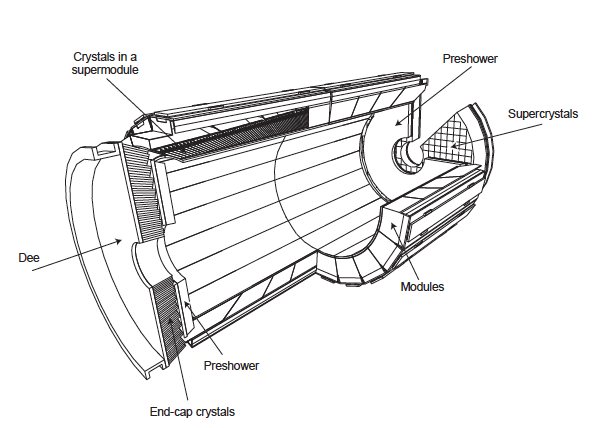
\includegraphics[width=1.0\columnwidth]{figures_chapter3/cms_ecal}
\caption{The layout of the CMS electromagnetic calorimeter. The barrel and endcap calorimeters are shown. The pre-shower detector sits in front of the endcap ecal.}
\label{fig:ecal}
\end{figure}

Figure~\ref{fig:ecal} shows the layout of the ECAL. The $61200$ crystals in EB are arranged in a $170\times360$ $\eta-\phi$ grid with a coverage up to $|\eta|=1.479$ in presudorapidity. The crystal front face cross section is approximately $0.0174\times0.0174$ in $\eta-\phi$ ($22-22$ mm$^2$) and $26-26$ mm$^2$ at the rear face. The increase in cross sectional area of the rear face is consistent with the small Moliere radius allowing to contain the transverse development of the electromagnetic shower within few crystals with respect to the central crystal. Each crystal has a length of $230$ mm corresponding to $25.8$ radiation lengths allowing to contain the longitudinal shower development with negligible levels of leakage. The crystals make an angle of $3$ degrees with respect to the particle trajectories incident from the interaction vertex to avoid cracks aligned with the trajectories. Two avalanche photodiodes (APDs) with an active are of $5\times5$ mm$^2$ are connected to the back of the crystals to convert the scintillation light to photo-electrons.   

The $14648$ crystals in EE are arranged in an $x-y$ grid with a front face cross section of $28.62\times28.62$ mm$^2$ and a rear face cross section of $30\times30$ mm$^2$. The length of the crystals is $220$ mm corresponding to $24.7$ radiation lengths. Vacuum phototriodes (VPTs) with an active area of approximately  $280$ mm$^2$, allowing large surface coverage, are used as photodetectors. An anode of very fine copper mesh allows to operate these devices in the $3.8$ Tesla magnetic field with only slight lose in gain. The EE extends the ECAL coverage from $|\eta|=1.479$ to $|\eta|=3.0$. A sampling preshower detector sits in front of the EE allowing the identification of neutral pions from $|\eta|=1.7$ to $|\eta|=2.6$. Two alternating layers of passive led and active silicon layers form a sampling calorimeter with approximately $3$ radiation lengths of the absorber material.  

The energy resolution of the ECAL can be parameterized as
\begin{equation} \label{eq:ecal_resol}
\frac{\sigma}{E} = \frac{S}{\sqrt{E}} \oplus  \frac{N}{E} \oplus C,
\end{equation}
where $E$ is the energy of the incident particle, $S$ is the stochastic term, $N$ is the noise term, and $C$ is the constant term. The longitudinal shower leakage is assumed to be negligible in (\ref{eq:ecal_resol}). Event-to-event fluctuations in the lateral shower containment and the photo-statistics of $2.1\%$ contribute to the stochastic term. The noise term is mostly due to the electronic and digitization noise while the constant term comes from intercalibration errors and a non-uniform light collection. Typical values found at an electron test beam are $S=0.029~\GeV^{\frac{1}{2}}$, $N=0.12~\GeV$, and $C=0.003$.    

\section{Hadron calorimeter}

The goal of the CMS hadron calorimeter (HCAL)\cite{hcal} is to measure the energy of charged and neutral hadrons. This is particularly important for the measurement of hadronic jets and transverse missing energy. Figure~\ref{fig:hcal} shows the layout of the hadron calorimeter components in the $r-z$ coordinate plane. The HCAL barrel calorimeter (HB) sits behind the ECAL between a radius of $r=1.77$ m and the inner extend of the magnetic coil ($r=2.95$ m). The HB is a sampling calorimeter extending to $|\eta|=1.3$ in pseudorapidity with $0.087\times0.087$ segmentation in $\eta-\phi$. The first layer of the absorbing material is a $40$ mm thick steel plate followed by eight $50.5$ mm thick brass plates with a last layer of $75$ mm thick steel plate. The chemical composition of the non-magnetic brass is $70\%$ Cu and $30\%$ Zn with a radiation length of $1.49$ cm. Thus the total absorber thickness is $5.8$ interaction lengths ($\lambda_{I}$) at $\eta=0$ and increasing to $10.6$ $\lambda_{I} $ at $|\eta|=1.3$. It has to be noted that the ECAL in front of HB adds about $1.1$ $\lambda_{I}$  of additional material.      

\begin{figure}[h]
\centering
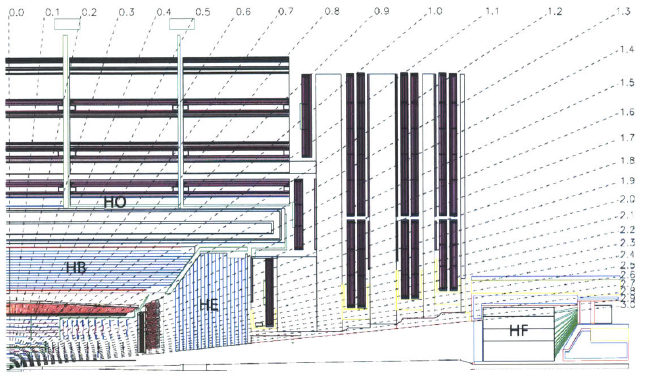
\includegraphics[width=1.0\columnwidth]{figures_chapter3/cms_hcal}
\caption{The layout of the CMS detector in the $r-z$ coordinate plane showing the location of the hadron barrel, endcap, outer, and forward calorimeters. The dashed lines show the extend of the coverage in pseudorapidity.}
\label{fig:hcal}
\end{figure}      

Plastic scintillators  ($3.7$ mm thick) are used for the active layers using a tile and wavelength shifting fiber setup to bring out the light. The first and last layers of the scintillators are $9$ mm thick where the latter serves to correct for the late developing hardon showers leaking out the back of the HB while the former serves to sample the hardon showers developed in the inert material between the EB and HB. Clear fibers are spliced onto the wavelength shifting fibers which are connected to optical fibers that take the light to an optical decoding unit (ODU). The role of the ODU is to arrange the fibers into read-out towers and bring the light to the hybrid photodiodes (HPDs)\cite{Cushman2000289}. The central component of the HPD is a photocathode held at a high voltage of $-8$ kV from a pixelated silicon photodiode.  The accelerated photo-electon from the cathode produces an ionization in the diode ($3.3$ mm away) with an overall gain of about $2000$. 

 The hadron endcap (HE) extends the pseudorapidity coverage to $|\eta|=3.0$ providing about $10$ $\lambda_{I}$ interaction lengths (including the ECAL crystals). The granularity of the HE is $0.087\times0.087$ in $\eta-\phi$ for $|\eta|<1.6$ and $0.17\times0.17$ for $|\eta|\geq 1.6$. The EB and HB absorbing power does not provide sufficient containment of the hadronic showers. An additional outer calorimeter (HO) that utilizes the solenoid  as an absorbing material is placed in the iron yoke (radial distance of $4.1$ m) that returns the solenoid magnetic field. There is an additional sensitive layer at a radial distance of $3.8$ m at $\eta=0$ as the HB has minimal absorbing length there. The total absorber thickness is increased to a maximum of $11.8$ $\lambda_{I}$ through the inclusion of the HO.
 
The forward calorimeter (HF) extends the pseudorapidity coverage to $|\eta|=5.2$. The HF is also responsible for the measurement of electromagnetic energy since the coverage of ECAL extends only to $|\eta|=3.0$.   
The particle flux in this region is extremely high; presenting a hostile conditions for the detector and requiring a radiation hard active material. Steel absorber layers and scintillating quartz fibers are used as the passive and active materials respectively. The absorption depth is approximately $10$ $\lambda_{I}$. Cherenkov light is generated in the quartz fibers when the charged shower particles are above the Cherenkov threshold. Thus the HF is mostly sensitive to the electromagnetic component of the showers. The HF has a longitudinal segmentation of two segments that allows to distinguish between incident electrons/photons and hadrons. This is accomplished by having two sets of fibers where one set only starts at a depth of $22$ cm from the front end of the detector. The transverse segmentation is $0.175\times0.175$ in $\eta-\phi$. The Cherenkov light is measured by a standard bialkaline  high gain photomultiplier tube with a borosilicate glass in the fringe magnetic field of the solenoid. 

\subsection{HCAL upgrades during the long shutdown $1$ and $2$}

There is a comprehensive program to upgrade the HCAL detectors to take advantage of technologies that have become available since the original design of the detector\cite{Mans:1481837}. The Phase $1$ upgrade of the CMS HCAL is designed to improve the performance of the calorimeters at high luminosities with mean number of about $50$ pileup events expected at the LHC. The HPDs in the HB and HE will be replaced by silicon photomultiplier (SIPM) devices while the single-channel phototubes in the HF will be replaced by multi-anode phototubes operated in a dual-anode configuration to reject spurious signals  present in the single-channel phototubes. The readout detectors of all the calorimeter detectors will be replaced as well. 

\begin{figure}[h]
\centering
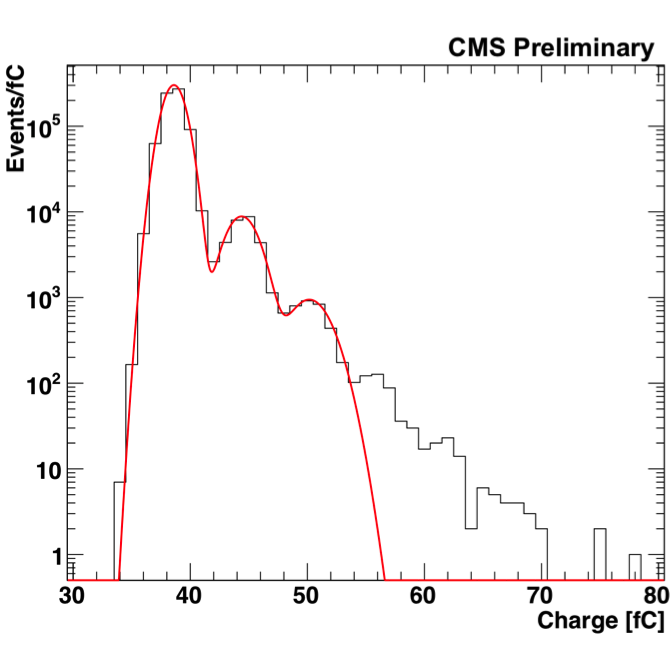
\includegraphics[width=0.6\columnwidth]{figures_chapter3/sipm2.png}
\caption{Charge distribution in a SIPM for events with no incident photons\cite{CMS-DP-2014-013}. The first peak is due to the leakage current while the subsequent peaks show the thermal avalanches of individual pixels. The red curve is a fit to the charge distribution.}
\label{fig:sipm}
\end{figure}

The Phase $1$ upgrade program will be carried out during the long shutdown $2$ (LS2) starting in $2018$. However, the HPDs in the HO calorimeter were already replaced by SIPMs during LS1. SIPMs are pixel arrays of avalanche photodiodes each operating in Geiger mode. Adding the signal of all the pixels together gives a measurement of the number of incident photons. SIPMs are compact devices that operate at about $2$ orders of magnitude lower voltages compared to the HPDs. The gain is similar to that of photomultipliers but the quantum efficiencies are a factor of $2$ higher compared to the HPDs. In addition, the SIPMs are not affected by magnetic fields of up to $4$ Tesla while about $10\%$ of the HPDs experience rapid breakdown at lower magnetic fields affecting the HO calorimeter in the fringe fields outside of the solenoid. 

SIPMs have an order of magnitude higher signal to noise ratios compared to the HPDs. The low signal to noise ratio is evident in Figure~\ref{fig:sipm} showing the thermal avalanches of individual pixels. The performance of the SIPM devices allows to increase the depth segmentation of the HB and HE calorimeters. The current depth segmentation is summarized in Figure~\ref{fig:depth}. The current HB calorimeter has a single longitudinal readout for most of the towers.  
 
\begin{figure}[h]
\centering
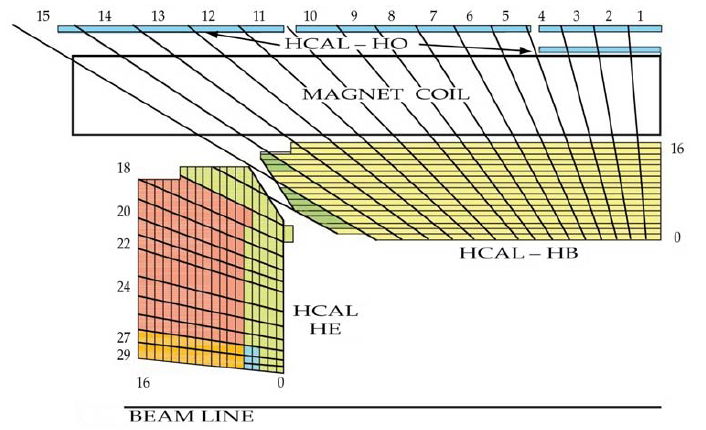
\includegraphics[width=1.0\columnwidth]{figures_chapter3/depth}
\caption{The current HCAL segmentation in the $r-z$ coordinate plane. The grouping of colors represents the optical grouping of the scintillator layers into different readouts.}
\label{fig:depth}
\end{figure} 
 
\section{Muon Detectors}

The goal of the CMS muon detectors~\cite{cms_muon} is threefold: muon triggering, identification, and the momentum measurement. Muons are minimum ionizing particles and there is little energy loss due to bremsstrahlung as muons have about $200$ times larger mass than electrons. Muons are detected in gas-ionization detectors embedded in the the steel return yoke outside of the solenoid. An appearance of a charged particle in the muon detectors is a strong indication of a muon particle as the charged hadrons, electrons, and photons are effectively stopped by the ECAL and HCAL.   

The layout of the CMS muon system is shown in Figure~\ref{fig:muon_layout} providing a pseudorapidity overage to $|\eta|=2.4$. Drift tube (DT) chambers with rectangular drift cells are used in the central barrel region with a pseudorapidity coverage to $|\eta|=1.2$. There are $4$ stations cylindrically interspersed in the layers of the flux return plates where the first $3$ stations contain $8$ chambers measuring the muon coordinate in the $r-\phi$ plane and $4$ chambers providing a measurement in the $z$ direction along the beam-line. The last station does not have the $z$ measurement plates. The gas used in the drift cells is a mixture of argon and carbon dioxide. The maximum drift time is $380$ ns in this mixture corresponding to a drift length of $21$ mm.  

\begin{figure}[h]
\centering
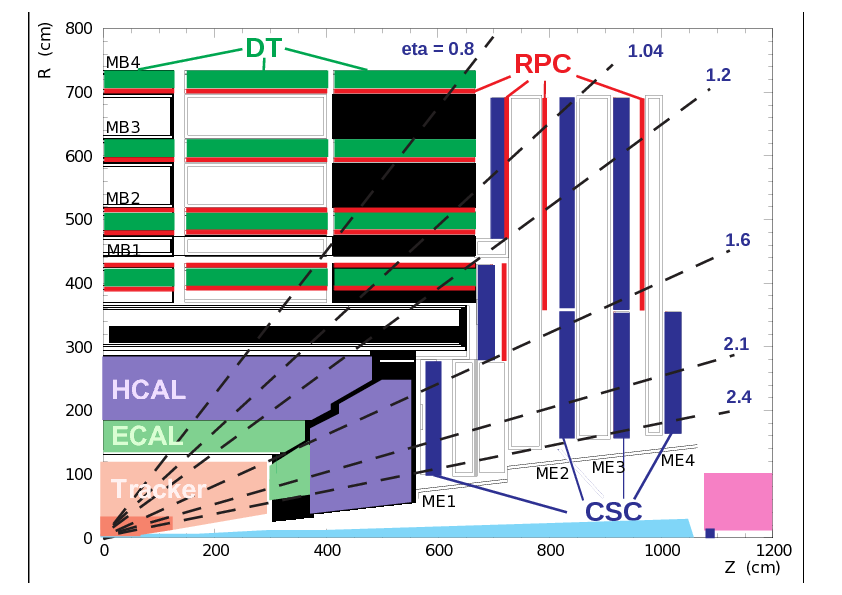
\includegraphics[width=1.0\columnwidth]{figures_chapter3/cms_muon_layout}
\caption{The layout of the CMS detector in the $r-z$ coordinate plane showing the location of the four DT chambers in the barrel (MB1-MB4) and the four CSC chambers in the endcap (ME1-ME4). The RPC stations are shown in red\cite{Chatrchyan:2012xi}. The dashed lines show the extend of the coverage in the pseudorapidity.}
\label{fig:muon_layout}
\end{figure}   

Cathode strip chambers (CSCs) are used in the endcap region, where the muon rates and background levels are higher, with a pseudorapidity coverage from $|\eta|=0.9$ to $|\eta|=2.4$. The CSCs are radiation resistant and have a fast response time and fine segmentation. There are $4$ stations with chambers positioned perpendicular to the beam line with the cathode strips of each chamber running radially outward to provide measurements in the $r-\phi$ plane. The anode wires are also read out. They run perpendicular to the strips and provide measurements in $\eta$. 

A dedicated trigger system consisting of resistive plate chambers (RPCs) is added covering up to $|\eta|=1.6$ in pseudorapidity. The RPCs are double-gap chambers that operate in avalanche mode. The response is very fast with a time resolution of about $1$ ns. They serve as an independent muon trigger system that can identify the correct bunch crossing time at the LHC nominal instantaneous luminosity. The position resolution of the RPCs is  poorer than the DTs and CSCs. 

\begin{figure}[h]
\centering
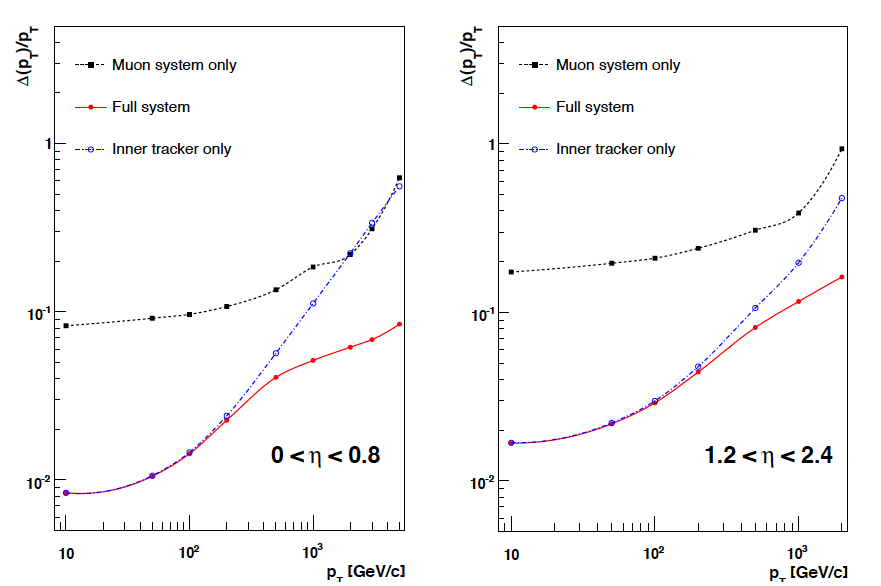
\includegraphics[width=1.0\columnwidth]{figures_chapter3/momentum_resolution}
\caption{The expected muon transverse momentum resolution as a function of the transverse momentum for $|\eta|<0.8$ (left panel) and $1.2<|\eta|<2.4$ (right panel)\cite{Chatrchyan:2008aa}. The performance for the muon system only (black), the inner tracker only (blue), and the full system (red) is shown.}
\label{fig:muon_resolution}
\end{figure}  

Figure~\ref{fig:muon_resolution} shows the expected muon transverse momentum resolution using the standalone muon system (black) and the inner tracking system (blue). A muon resolution of about $9\%$ for muon transverse momenta up to $200~\GeV$ is achieved. Multiple-scattering in the detector material before the first muon station limits the resolution achieved by the standalone muon system. An order of magnitude improvement in resolution is achieved using the inner tracker information in a global momentum fit, as described in the next chapter (red curves in Figure~\ref{fig:muon_resolution}).     

\section{Triggering and Data Acquisition}

The design $25$ ns bunch spacing at the LHC translates to a bunch crossing rate of $40$ MHz. This results in a total inelastic collision rate of order of $1$ GHz taking the additional inelastic proton-proton interactions per bunch crossing into account. A drastic rate reduction has to be achieved as it is impossible to store and process the resulting large amount of data. This is achieved by the triggering system. The triggering of the events in the CMS is achieved in two steps designated as Level One Trigger (L1)\cite{Bayatyan:706847,Khachatryan:2016bia} and High-Level Trigger (HLT)\cite{Khachatryan:2016bia,Cittolin:578006,Adam:2005zf}. The L1 trigger consists of a custom designed and largely programmable electronics while the HLT is a software system consisting of a farm of about one thousand commercial processors having a few thousand CPU cores. The L1 trigger takes the decision to either reject or accept the event for further evaluation by the HLT. Thus the events are readout and fully assembled only for the events that pass the L1 trigger. The readiness of the sub-detectors and the data acquisition (DAQ) system are considered in the L1 decision through the Timing, Trigger, and Control (TTC) system\cite{Varela:687458}. Finally the events are either discarded or passed to the offline computing system for storage and reconstruction depending on the HLT decision. The nominal output rate of the L1 trigger is $100$ kHz limited by the CMS readout electronic speed.  The HLT selects an average rate of $400$ Hz for storage and processing. However HLT accept rates of up to several kHz are possible if the data is not processed promptly. An extra $300-400$ Hz data was collected through special "parked" data stream\cite{CMS-DP-2012-022} during the $2012$ data taking period and reconstructed only at the end of the run. The overall output rate of the L1 trigger and HLT can also be adjusted by applying a pre-scale on the number of events that satisfy the selection criteria of specific algorithms. 

\begin{figure}[h]
\centering
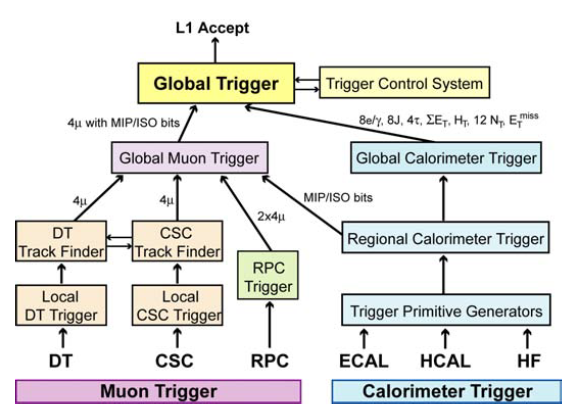
\includegraphics[width=0.8\columnwidth]{figures_chapter3/l1trig}
\caption{Level-1 trigger architecture showing the components of the trigger\cite{Chatrchyan:2008aa} .}
\label{fig:l1trig}
\end{figure}  

The L1 trigger uses coarsely segmented data from the calorimeters and the muon system. The full detector information is retained in the pipelined memory buffers of the front-end read-out electronics pending the L1 trigger decision. It has to be noted that no information from the inner tracking system is used in the L1 trigger as the number of channels and the speed of the readout electronics of the inner tracking detectors is currently prohibitive. The L1 hardware  is implemented in combination of Field Programmable Gate Arrays (FPGAs) and Application Specific Integrated Circuits (ASICs). A programmable memory lookup table (LUT) is also used where density and radiation requirements are important. The allowed latency is $3.2$ $\mu$s. Figure~\ref{fig:l1trig} shows the L1 trigger architecture and the information flow toward the L1 decision. The L1 trigger objects consist of clusters of the ECAL and HCAL deposits (photons/electrons, hadrons), muons, and global event information such as the summed transverse energy or the missing transverse energy. 

The HLT has access to the complete read-out data including the hit patterns from the inner tracking detector. Thus better position and momentum resolutions can be used compared to the L1 trigger objects. The HLT uses identical software framework to the one used in the offline processing. However optimized algorithms and configurations are used to manage the input rate of $100$ kHz. For example, reconstruction of the tracks in the inner tracking system is only performed after other selection criteria based on the calorimeter and muon detector information to reduce the CPU usage. In addition, the data is reconstructed in the regions of interest, defined by the L1 trigger information, to further reduce the processing time.  The output rate of the HLT is limited by event sizes and the capacity of the downstream systems to process the events. 

  




%% This is an example first chapter.  You should put chapter/appendix that you
%% write into a separate file, and add a line \include{yourfilename} to
%% main.tex, where `yourfilename.tex' is the name of the chapter/appendix file.
%% You can process specific files by typing their names in at the 
%% \files=
%% prompt when you run the file main.tex through LaTeX.
\chapter{Event Reconstruction}

The $W^{\pm}$ and $Z$ boson cross section measurements and $H \rightarrow \tau\tau$ searches rely on the precise reconstruction of the decay products. The presence of neutrinos in the leptonic $W$ decays and also in  $\tau$ decays requires an accurate reconstruction of all the detector deposits to infer the presence of the neutrinos from the momentum imbalance in the transverse plane. In addition, reconstruction of jets is important to capture the different production modes of the Higgs boson. The additional pileup interactions in the events present a challenge for a precise reconstruction of the events. This chapter summarizes the event reconstruction emphasizing the components relevant for the results that follow.

\section{Track Reconstruction}

The goal of the track reconstruction is to estimate the position and momentum parameters of charged particles from the reconstructed hits in the inner tracking detector. Reconstructing tracks at the LHC nominal instantaneous luminosities is a computationally challenging task due to a high occupancy environment. About $1000$ charged particles transverse the inner tracking detectors at each bunch crossing. Charged particles from prior or later bunch crossings can also be present due to finite detector time resolution.  The track reconstruction starts by clustering of zero-suppressed signals in the pixel and strip detectors into hits. Each hit provides an estimate of the cluster position and the corresponding uncertainty. The CMS track reconstruction algorithm is referred to as combinational track finder (CTF)~\cite{Adam:934067,Chatrchyan:2014fea}. The CTF is an adaptation of the combinatorial Kalman filter~\cite{BILLOIR1989390,BILLOIR1990219,MANKEL1997169}, which is an extension of the Kalman filter~\cite{FRUHWIRTH1987444}, combining pattern recognition and track fitting in the same framework. 

The CTF is performed iteratively six times to determine the collection of the tracks in an event. The aim of this iterative tracking is to first find the tracks that are easiest to find (tracks with high $p_{T}$ and near the interaction region) with subsequent iterations searching for the more challenging tracks (tracks with low $p_{T}$ and displaced from the interaction region). Hits associated with tracks are removed after each iteration thereby reducing the computational complexity. Each iteration has four steps:

\begin{description}
\item[$\bullet$ Seed generation:]  Initial track candidates are found using only two or three hits in the inner part of the tracker. One has to note that the seeds are not constructed from the outermost regions of the tracker where the track density is small. The high granularity of the pixel detector ensures that the channel occupancy is lower than the channel occupancy of the outer strip layers. In addition, significant fraction of charged pions undergo inelastic interaction in the track detectors while many electrons loose significant energy due to bremsstrahlung radiation as they transverse the inner tracker. Five parameters are needed to define the helical trajectory of the charged particles in the approximately uniform magnetic field. Two or three hits in combination with a constrain on the origin of the charged particle to be near the beam spot (the three dimensional profile of the luminous region of the collisions) is sufficient to extract these parameters.
\item[$\bullet$ Track finding:]  The Kalman filter algorithm is used to provide a coarse estimate of the track parameters starting from the seeds. A track candidate is built by adding hits from successive detector layers. A fast analytical propagator is used to find the hit layers. The track parameters are updated each time a new hit is found.
\item[$\bullet$ Track fitting:] The full information needed for the trajectory is only available once all the hits of the trajectory are identified. Therefore, the trajectory is once again re-fitted using a Kalman filter and smoother. A fourth-order Runge-Kutta method is used to extrapolate the trajectory between the successive hits. Material and inhomogeneous magnetic field effects are included.
\item[$\bullet$ Track selection:] Quality requirements are applied to reject fake tracks not originating from charged particles. 
\end{description}

The track reconstruction is effectively fully efficient for isolated muons with $2.5\%$ resolution in $p_{T}$ for $p_{T}$ of about $100~\GeV$~\cite{Chatrchyan:2014fea}. The longitudinal (with respect to the $z$ axis) and transverse impact parameter resolutions are $30$ $\mu$m and $10$ $\mu$m respectively. The efficiency for charged particles of $p_{T}$ greater than $0.9~\GeV$ in simulated $t\bar{t}$ events is $94\%$ ($85\%$) in the pseudorapidity region of $|\eta|<0.9$ ($0.9<|\eta|<2.4$). The main cause of the inefficiency is due to the hadrons undergoing nuclear interactions in the tracker material.   

\section{Primary Vertex Reconstruction}

The goal of the primary vertex reconstruction is to measure the position of each proton-proton interaction vertex in each event. The vertex reconstruction starts from the collection of the reconstructed tracks consistent with being produced near the beam spot. Additional quality requirements on the number of inner tracker layers associated to the track and the quality of the CTF fit are applied. There is no requirement on the $p_{T}$ of the tracks ensuring high vertex reconstruction efficiency.

A clustering algorithm based on the $z$ coordinates of closest approach of the tracks to the beam spot is used to resolve the vertices. The tradeoff is to be able to resolve the nearby vertices against the accidental splitting of a single vertex into more than one cluster of tracks.  A deterministic annealing (DA) algorithm~\cite{726788} is used for the clustering where the most probable vertex positions are found through a minimization of "free energy" $F$ at "temperature" $T$~\cite{Chatrchyan:2014fea}, 
\begin{equation} \label{eq:minimize}
F = -T \sum_{i}^{N_{T}} \ln \sum_{j}^{N_{V}} p_{ij} \rho_{j} \exp  \left[-\frac{1}{T}\frac{(z_{i}^{T}-z_{j}^{V})^2}{{\sigma_{i}^{z}}^2} \right],
\end{equation}
where $z_{i}^{T}$ and $\sigma_{i}^{z}$ are the $z$ coordinates of the points of the closest approach of the tracks to the $z$ and the corresponding uncertainties, $z_{j}^{V}$ are the vertex positions with vertex weights $\rho_{j}$, and $p_{ij}$ is the probability of assigning the track $i$ to the vertex $j$. The assignment of the probabilities is such that at very low temperatures every track is compatible with a single vertex while at very high temperatures all the tracks become compatible with a single vertex. The algorithm starts at a high temperature that gradually decreases ($F$ is minimized at each step) until a pre-defined minimum temperature is reached. Thereafter the temperature is further decreased to $T=1$ for the final assignment without further splitting of the vertices. 

\begin{figure}[h]
\centering
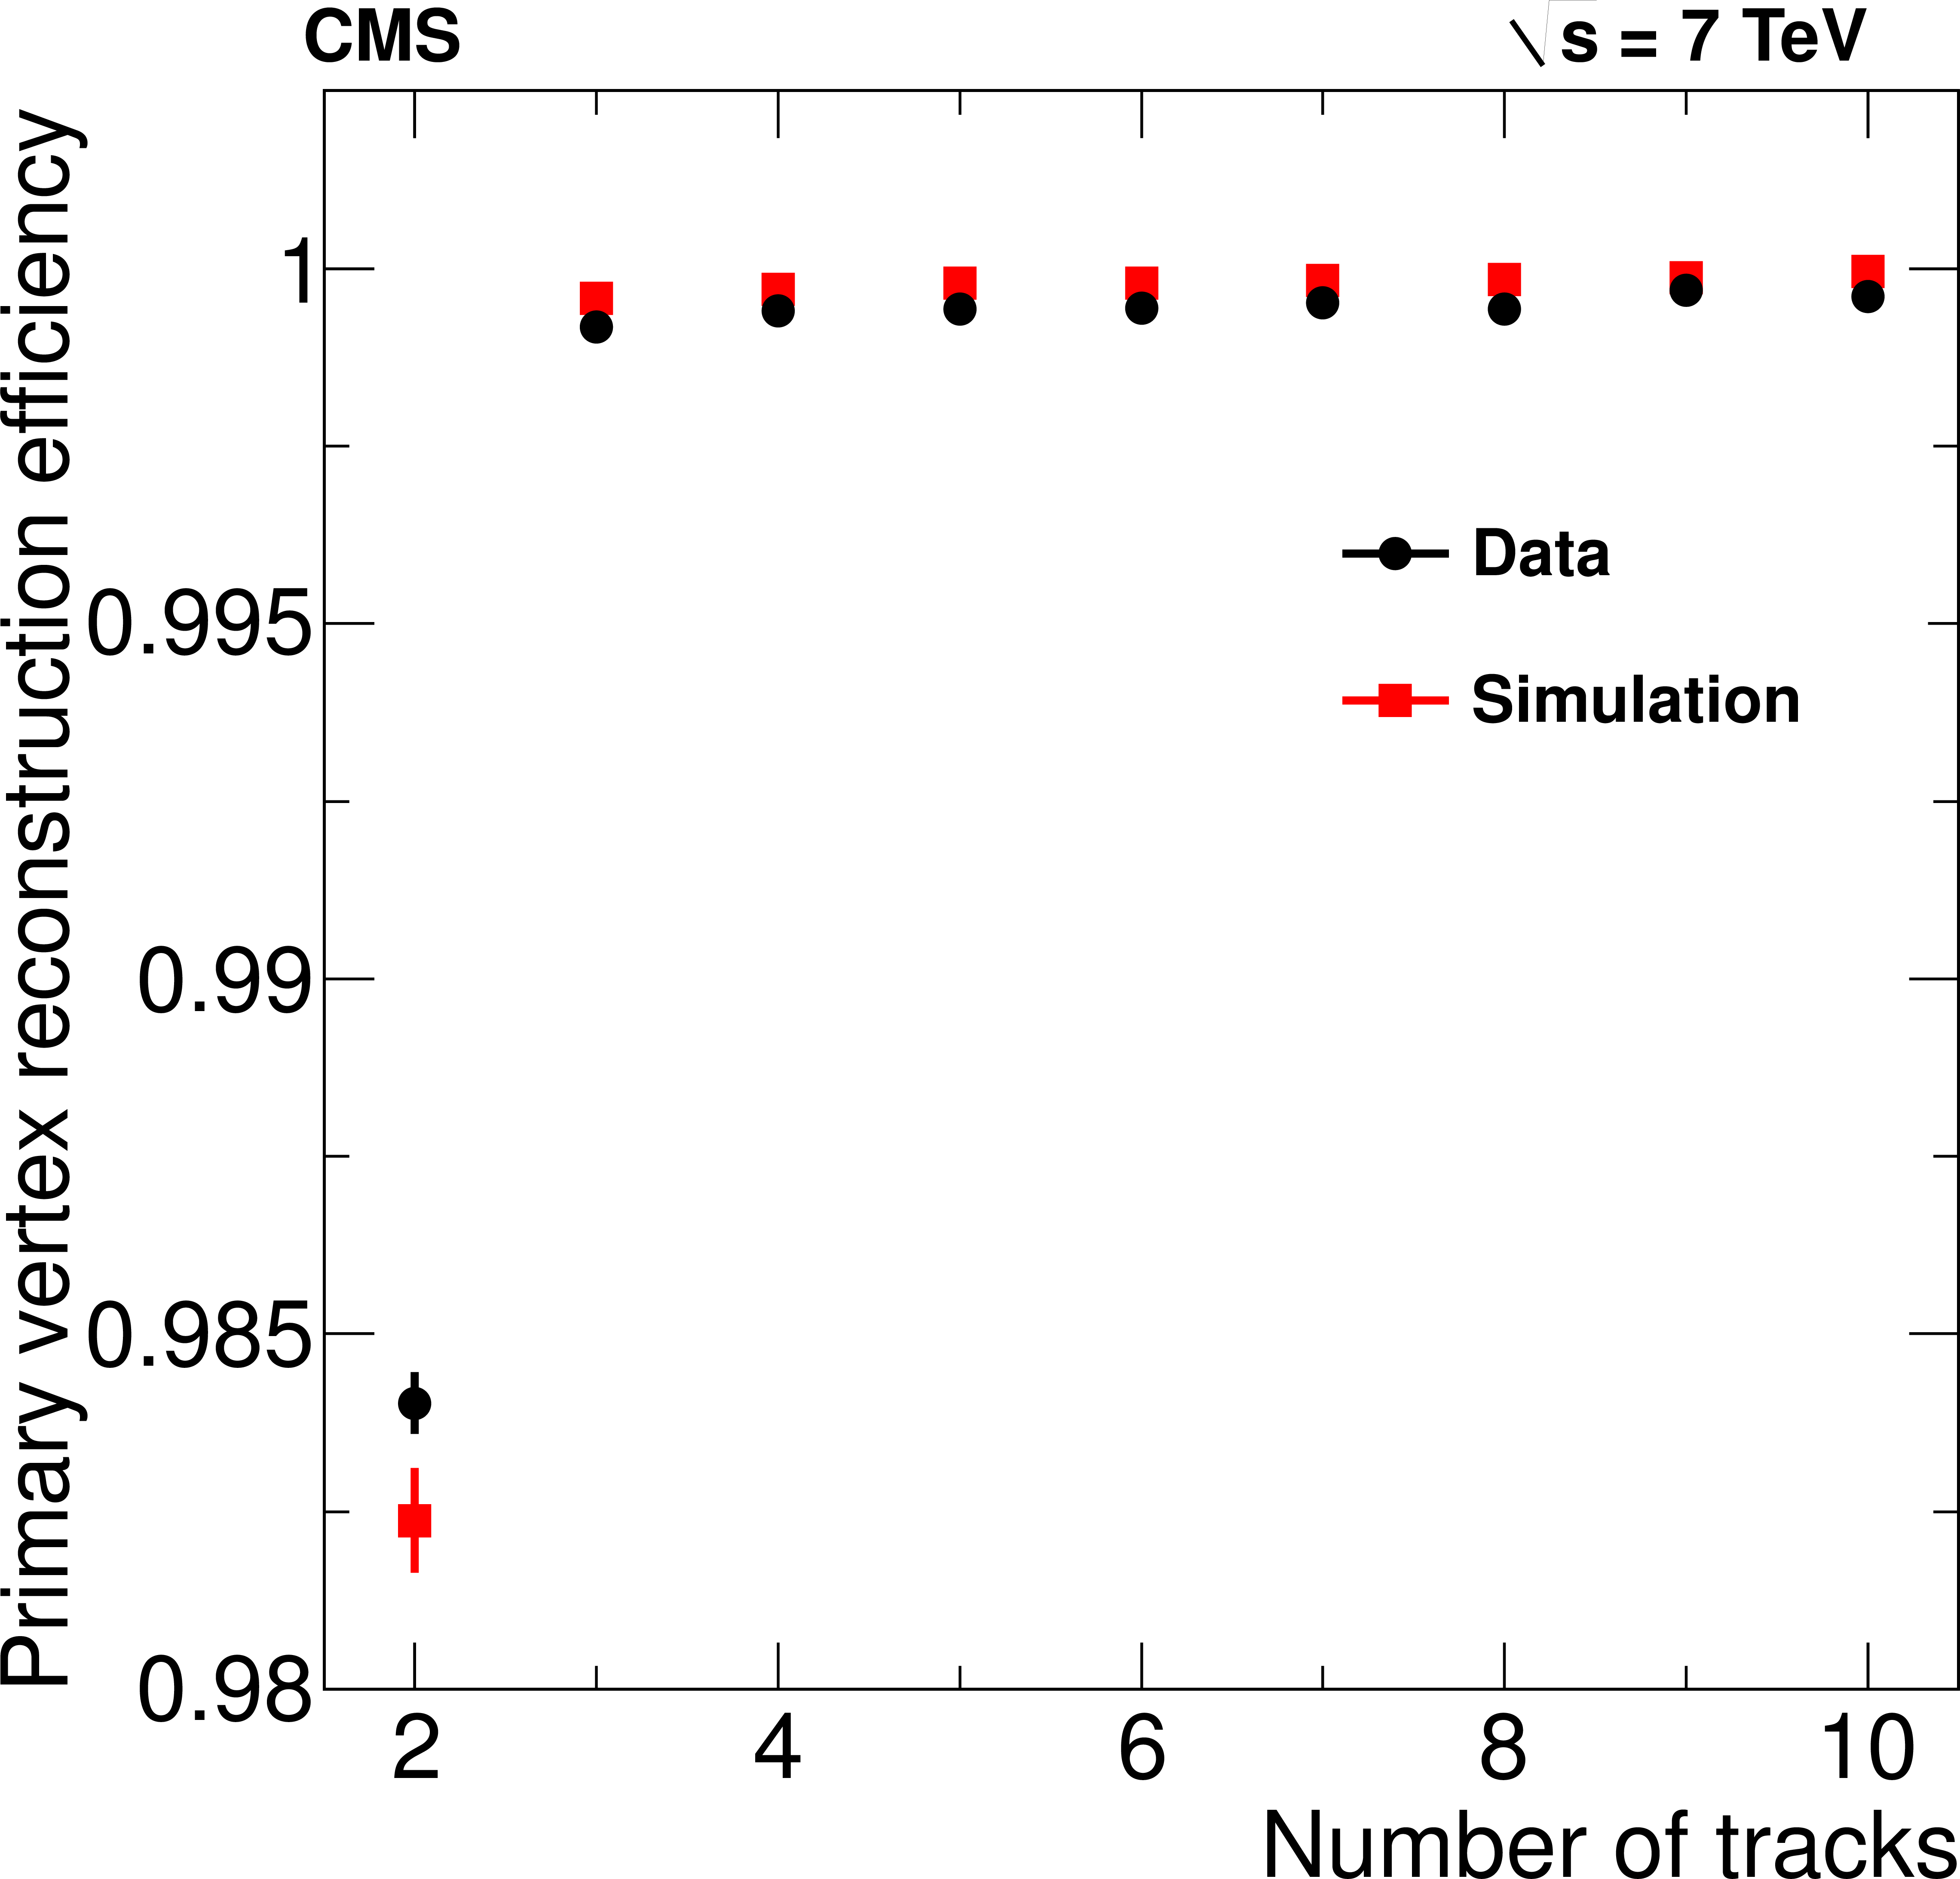
\includegraphics[width=0.49\columnwidth]{figures_chapter4/vertex_efficiency}
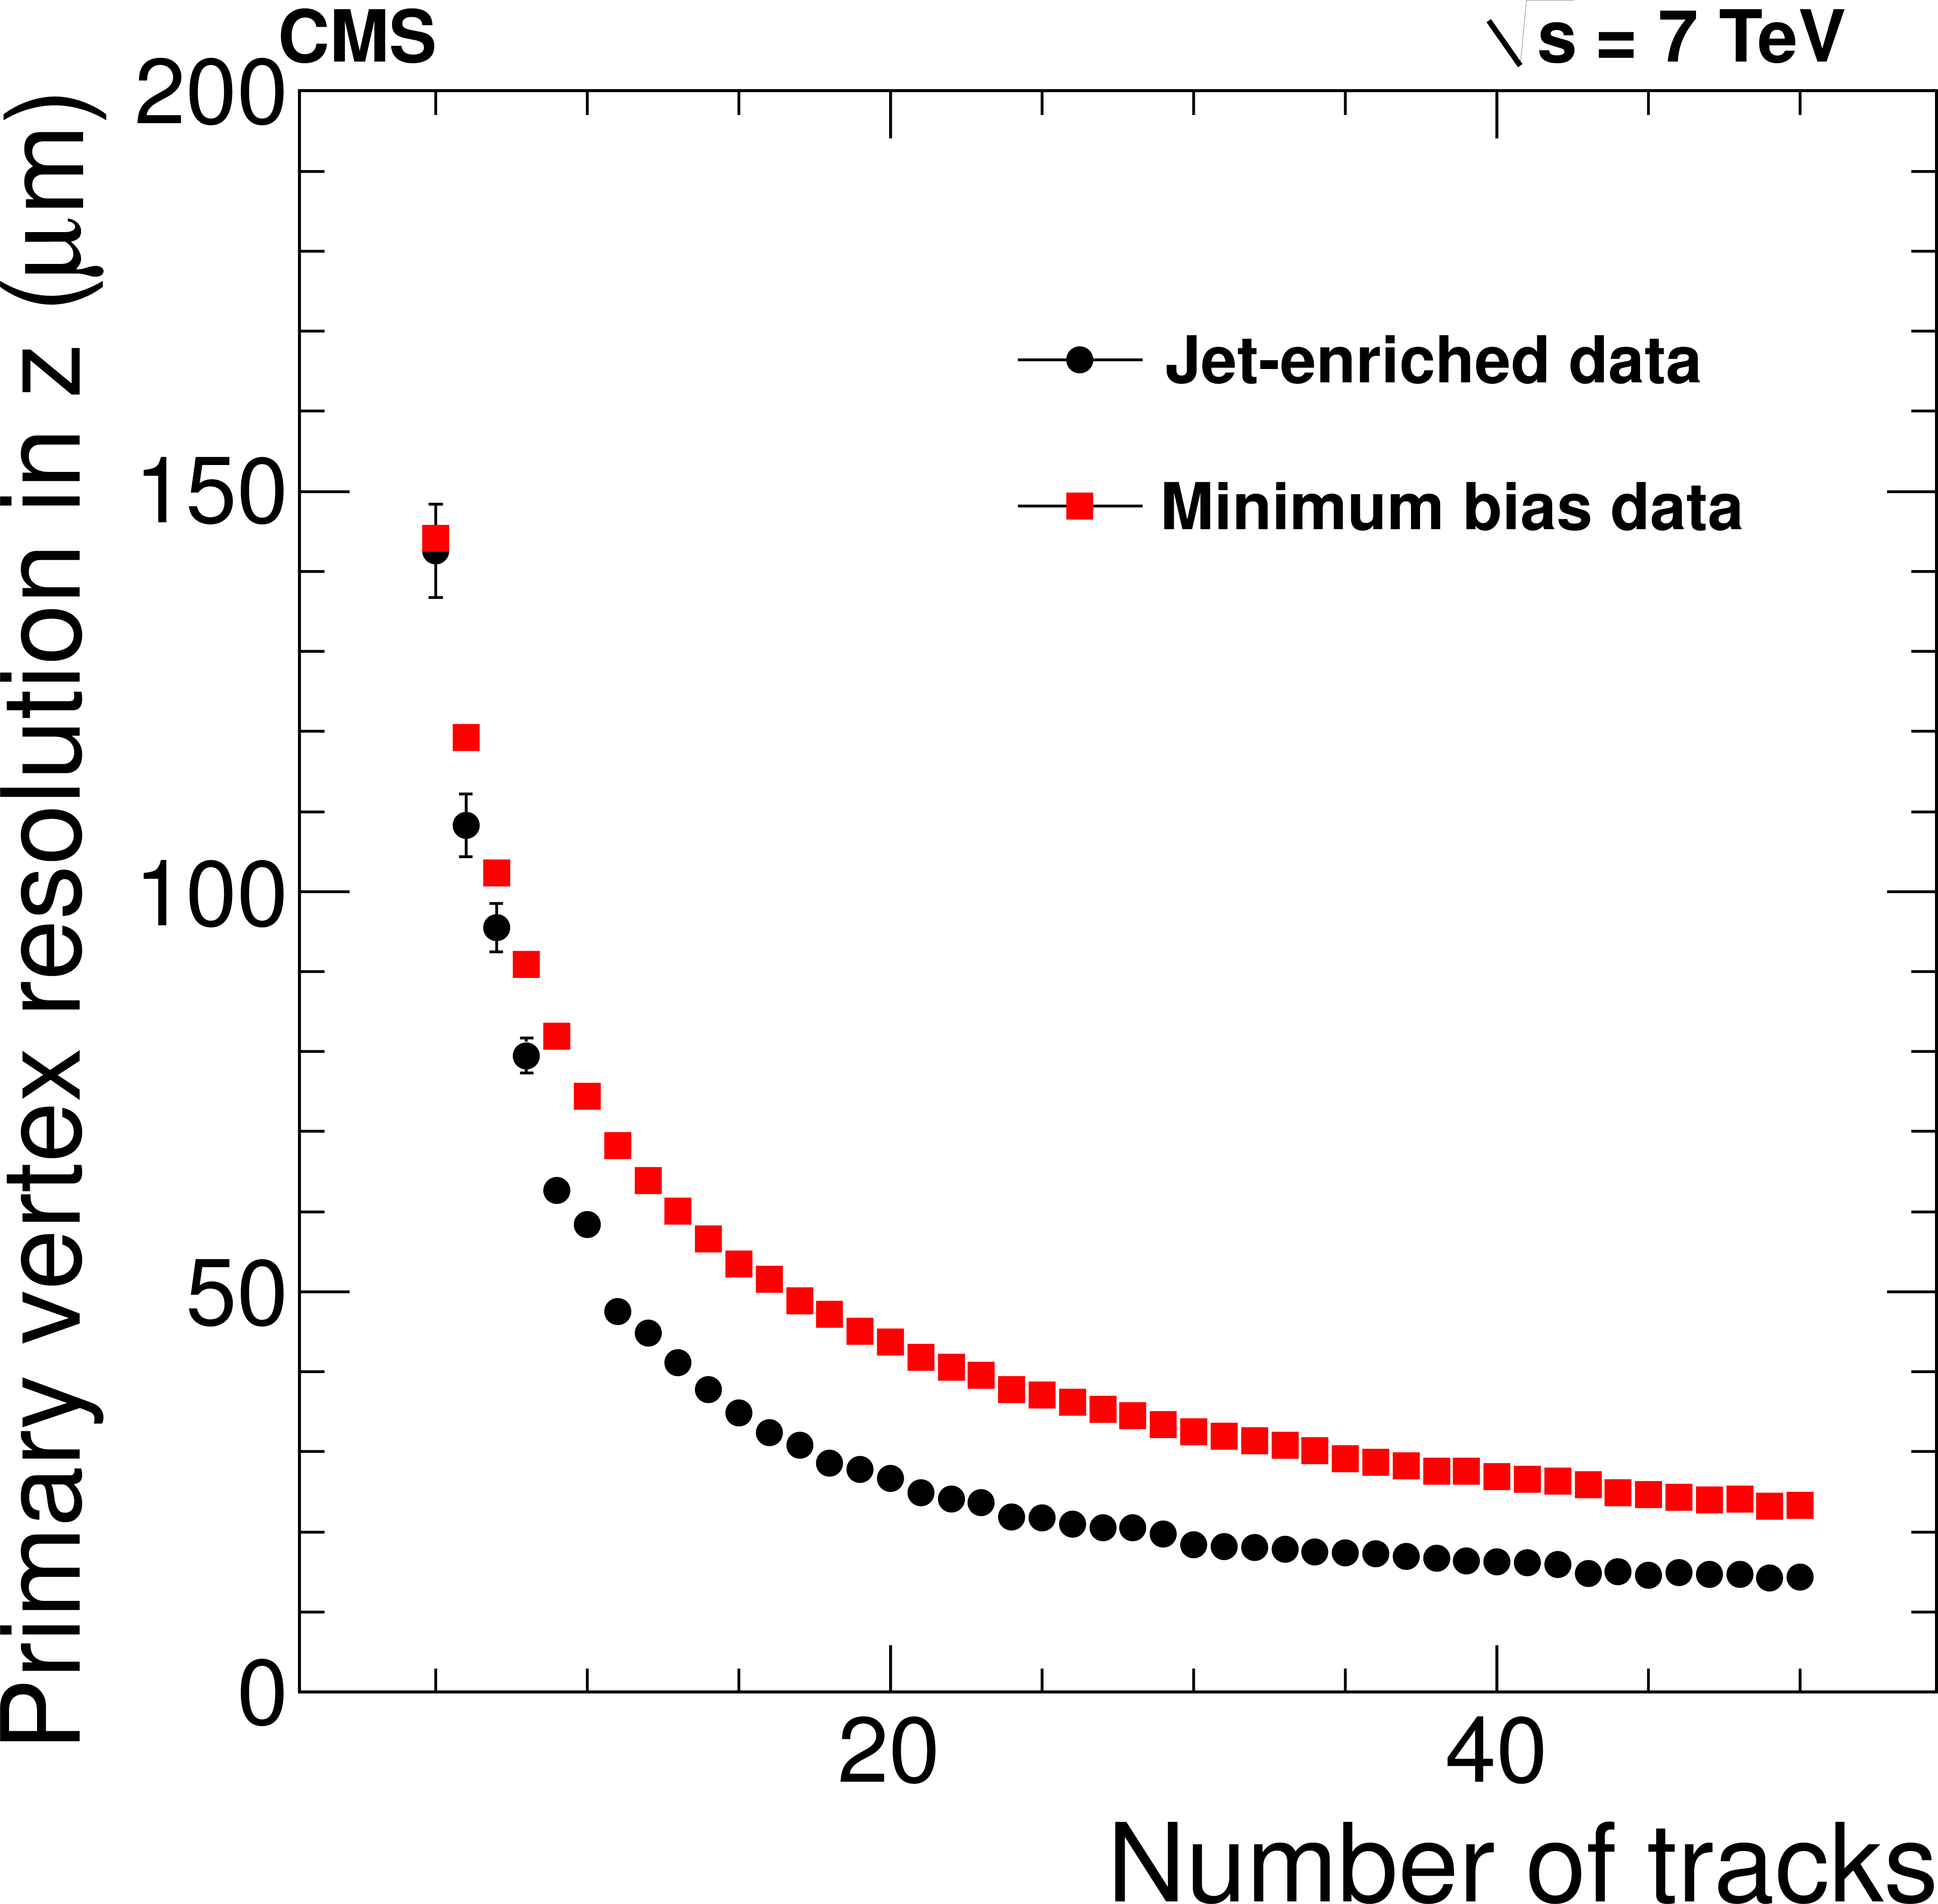
\includegraphics[width=0.49\columnwidth]{figures_chapter4/vertex_resolution}
\caption{Vertex reconstruction efficiency (left panel) as a function of the number of tracks in the vertex measured in minimum-bias data and in simulation. Vertex resolution (right panel) in the $z$ coordinate as a function of the number of tracks measured in minimum bias events (red) and jet-enriched events (black)~\cite{Chatrchyan:2014fea}.}
\label{fig:vertex}
\end{figure}

The candidate vertices determined by the DA clustering that contain at least two tracks are fitted using an adaptive vertex fitter~\cite{0954-3899-34-12-N01} to determine all the vertex parameters, including the $x$, $y$, and $z$ positions. Figure~\ref{fig:vertex} shows the vertex reconstruction efficiency (left) and vertex resolution in $z$ coordinate as a function of the number of tracks used to fit the vertex. The reconstruction efficiency is close to $100\%$ when there are more than two tracks used to reconstruct the vertex. The vertex resolution also depends on the number of tracks as well as the $p_{T}$ of the tracks. The vertex resolutions are shown for minimum bias data events (red), where loose triggers select inelastic pp collisions with as little bias as possible, and jet enriched data events, where the events are required to have a reconstructed jet with a transverse energy $E_{T}$ greater than $20~\GeV$ (black). The tracks in the jet enriched events have higher $p_{T}$ resulting in better vertex resolution. A resolution of approximately $10$ $\mu$m is achieved for high $p_{T}$ vertices with at least $50$ tracks.   

The vertex with the largest sum of the $p_{T}^2$ is defined to be the true hard-scattered pp vertex and is denoted as the primary vertex. The other vertices in the event are assumed to originate from the additional pileup interactions in the bunch crossing. Beam induced backgrounds can be rejected by applying compatibility requirements on the primary vertex with the nominal interaction point (the origin of the CMS coordinate system). The distance of the primary vertex in the $z$ direction (transverse direction) to the nominal interaction point is required to be less than $24$ cm ($2$ cm). The number of degrees of freedom of the primary vertex fit is also required to be greater than $3$.

\section{Muon Reconstruction and Identification}

Muon tracks are reconstructed not only in the CMS inner tracker but also independently in the muon system~\cite{Chatrchyan:2012xi}. The latter tracks are called standalone muon tracks. The standalone muon tracks are reconstructed from the hits in the muon chambers in a combined track fit using a Kalman filter. The "global muon" reconstruction refers to the combination and matching of the standalone muon tracks with the inner tracker tracks. A global muon track is fitted from these tracks again using a Kalman filter technique. The expected energy loss in the solenoid and support structures is taken into account in the fit. The global fit improves the momentum resolution for muons with $p_{T}$ greater than $200~\GeV$ compared to the inner tracker only resolution as demonstrated in Figure~\ref{fig:muon_resolution}.   

Another independent algorithm starts from the inner tracker and proceeds outward in the radial direction matching the hits in the muons chambers. This "tracker muon" reconstruction is more efficient for low momentum muons ($p < 5~\GeV$) compared to the global muon reconstruction as it only requires one muon segment hit in the muon chambers. The tracker muon reconstruction considers all the inner tracker tracks with $p_{T}$ greater than $0.5~\GeV$ as possible muon candidates. The average expected energy loses and multiple Coulomb scattering in the detector material are taken into account for the extrapolation to the muon system. 

\begin{figure}[h]
\centering
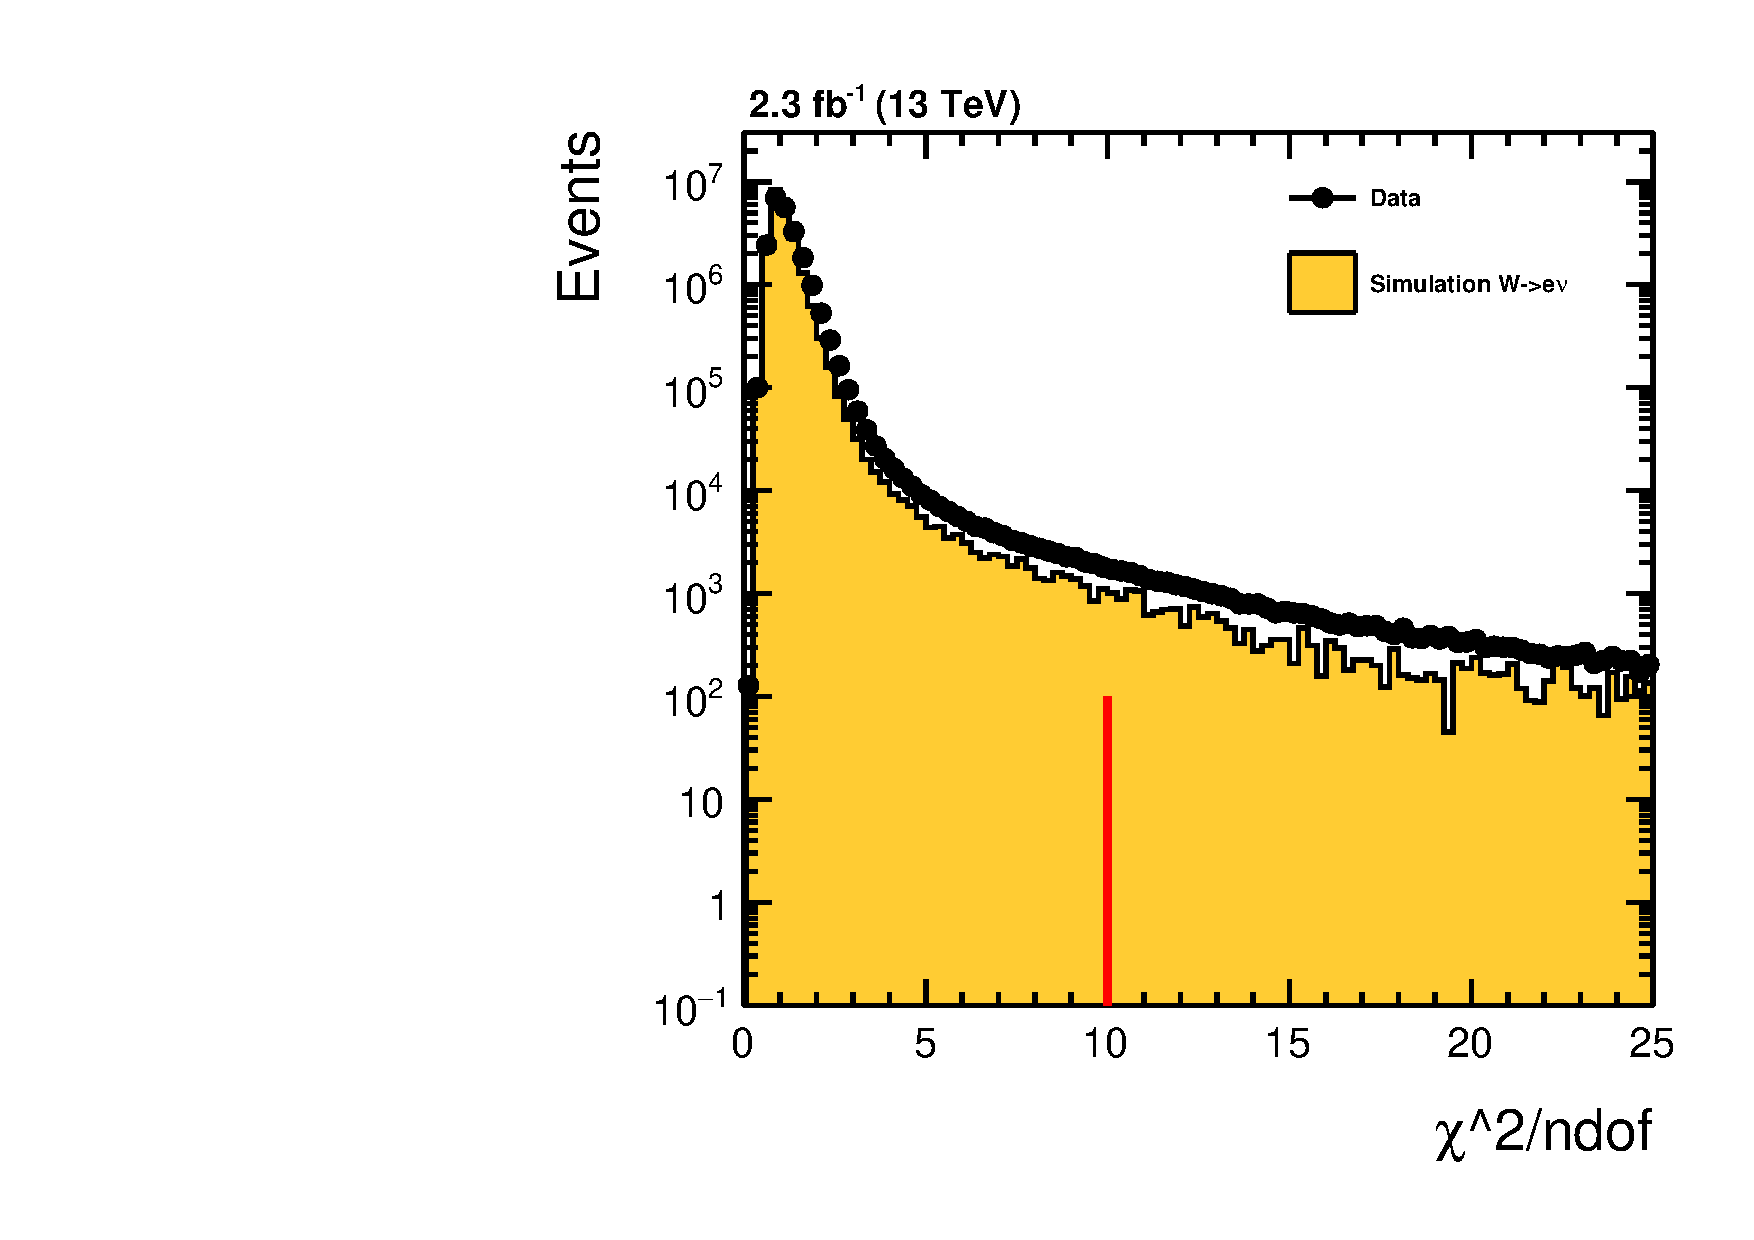
\includegraphics[width=0.49\columnwidth]{figures_chapter4/chi2_muon}
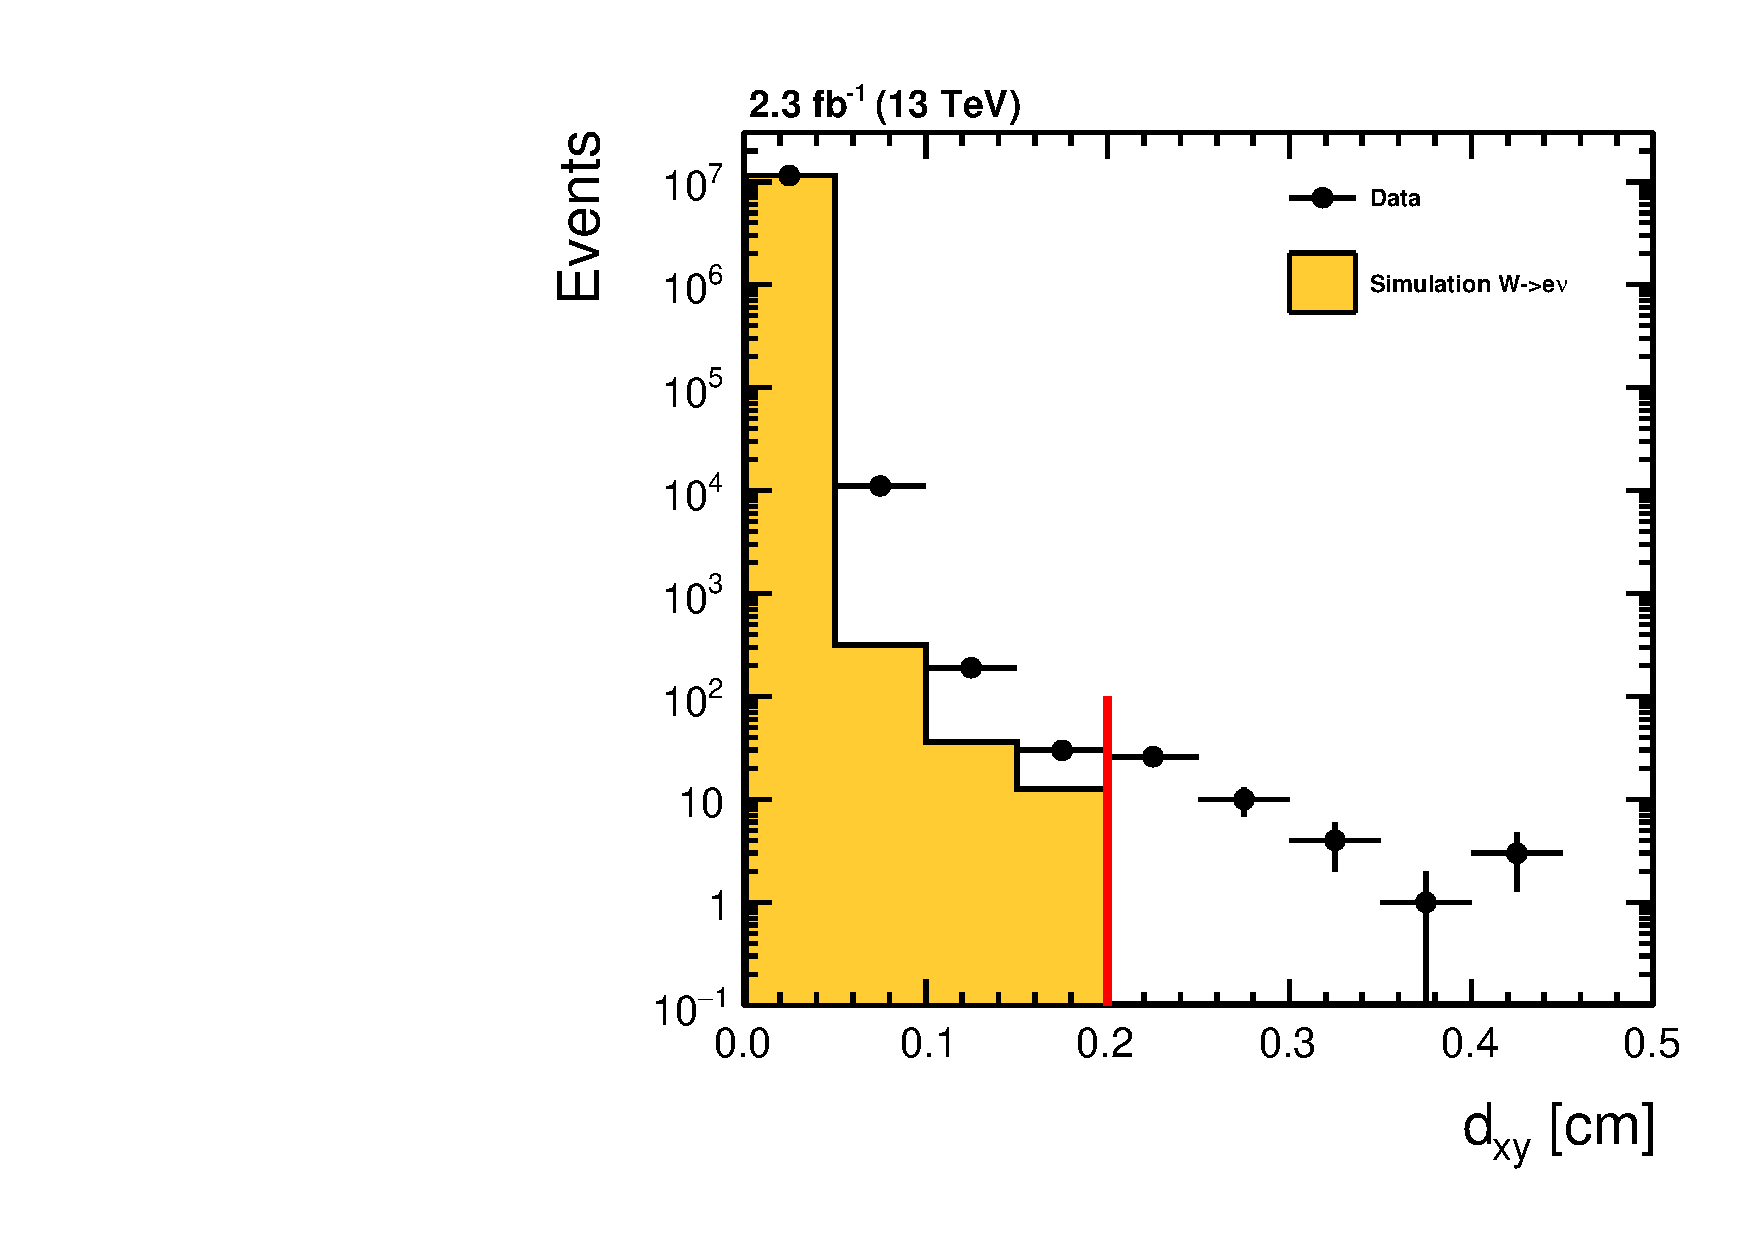
\includegraphics[width=0.49\columnwidth]{figures_chapter4/dxy_muon}
\caption{Distribution of $\chi^2$ per degree of freedom (left panel) and transverse impact parameter $d_{xy}$ (right panel) for data at $\sqrt{s}=13~\TeV$ taken during $2015$ data taking period. Simulated $W \rightarrow \mu \nu$ signal process normalized to the number of observed data evens is shown for comparison. The events satisfy all other selection requirements (including the isolation requirement to be discussed in Section 3.8) are satisfied except that on the shown variable. The red line illustrates the requirement on the variable for a selection optimized for that data-taking period.}
\label{fig:muon_id}
\end{figure}

Muon candidates selected in the results are required to be a global muon. Approximately $99\%$ of the muons in the fiducial volume (the geometrical acceptance) of the muon system are identified as either a tracker or a global muon. Muon candidates identified as both a global and a tracker muon are merged into a single candidate.  Additional quality requirements are imposed to reduce miss-identified muon candidates and so called non-prompt muons. Non-prompt muons originate from in-flight decays of light hadrons and semi-leptonic decays of the heavy flavor quarks. The miss-identified muon candidates originate from the punch-through of hadron showers to the muon system. The contribution is generally small for the global muons due to the minimum number of muon segment hits requirement. 

Figure~\ref{fig:muon_id} shows the distributions of few of the muon variables used for reduction of the non-prompt and miss-identified muons. The  $\chi^2$ per degree of freedom of the global track fit is required to be less than $10$. At least one segment in the muon stations must be included in the global fit to reduce the punch-through hadrons. The muons are required to have track segments in at least two muon stations. In addition, at least one hit in the pixel tracker and at least five tracking layers are required. Background originating from cosmic-ray muons transversing the CMS detector in coincidence with a pp collision is reduced by the impact parameter requirement. Figure~\ref{fig:muon_id} (right panel) shows the transverse impact parameter distribution $d_{xy}$ calculated with respect to the primary vertex. The candidates with large $d_{xy}$ originate mainly from the cosmic-ray muons. The excess of events with respect to the $W \rightarrow \mu\nu$ simulation is due to the in-flight decays of long lived particles in the QCD multi-jet background. There is also a requirement on the longitudinal impact parameter $d_{z}$ calculated with respect to the primary vertex of the event. 

\section{Electron Reconstruction and Identification}

Electrons are reconstructed by looking for a track in the inner tracker that is matched to energy deposits in the ECAL. Electron reconstruction is complicated due to \newline bremsstrahlung radiation emitted as the electrons transverse the inner tracker detector. These bremsstrahlung photons can subsequently undergo a pair-conversion before reaching the ECAL. As a result the electron energy reaching the ECAL is significantly spread in the azimuthal direction $\phi$ due to bending of the trajectories in the CMS magnetic field. Approximately $35\%$ of electrons radiate more than $70\%$ of their initial energy before reaching the ECAL~\cite{Chatrchyan:2014fea,Baffioni:2006cd}. A dedicated clustering algorithms are used to collect the bremsstrahlung energy taking the spreading in the $\phi$ direction into account~\cite{Meschi:687345}.  The spread in the $\eta$ direction is mostly negligible except for very low $p_{T}$ (less than $5~\GeV$).    

\begin{figure}
\centering
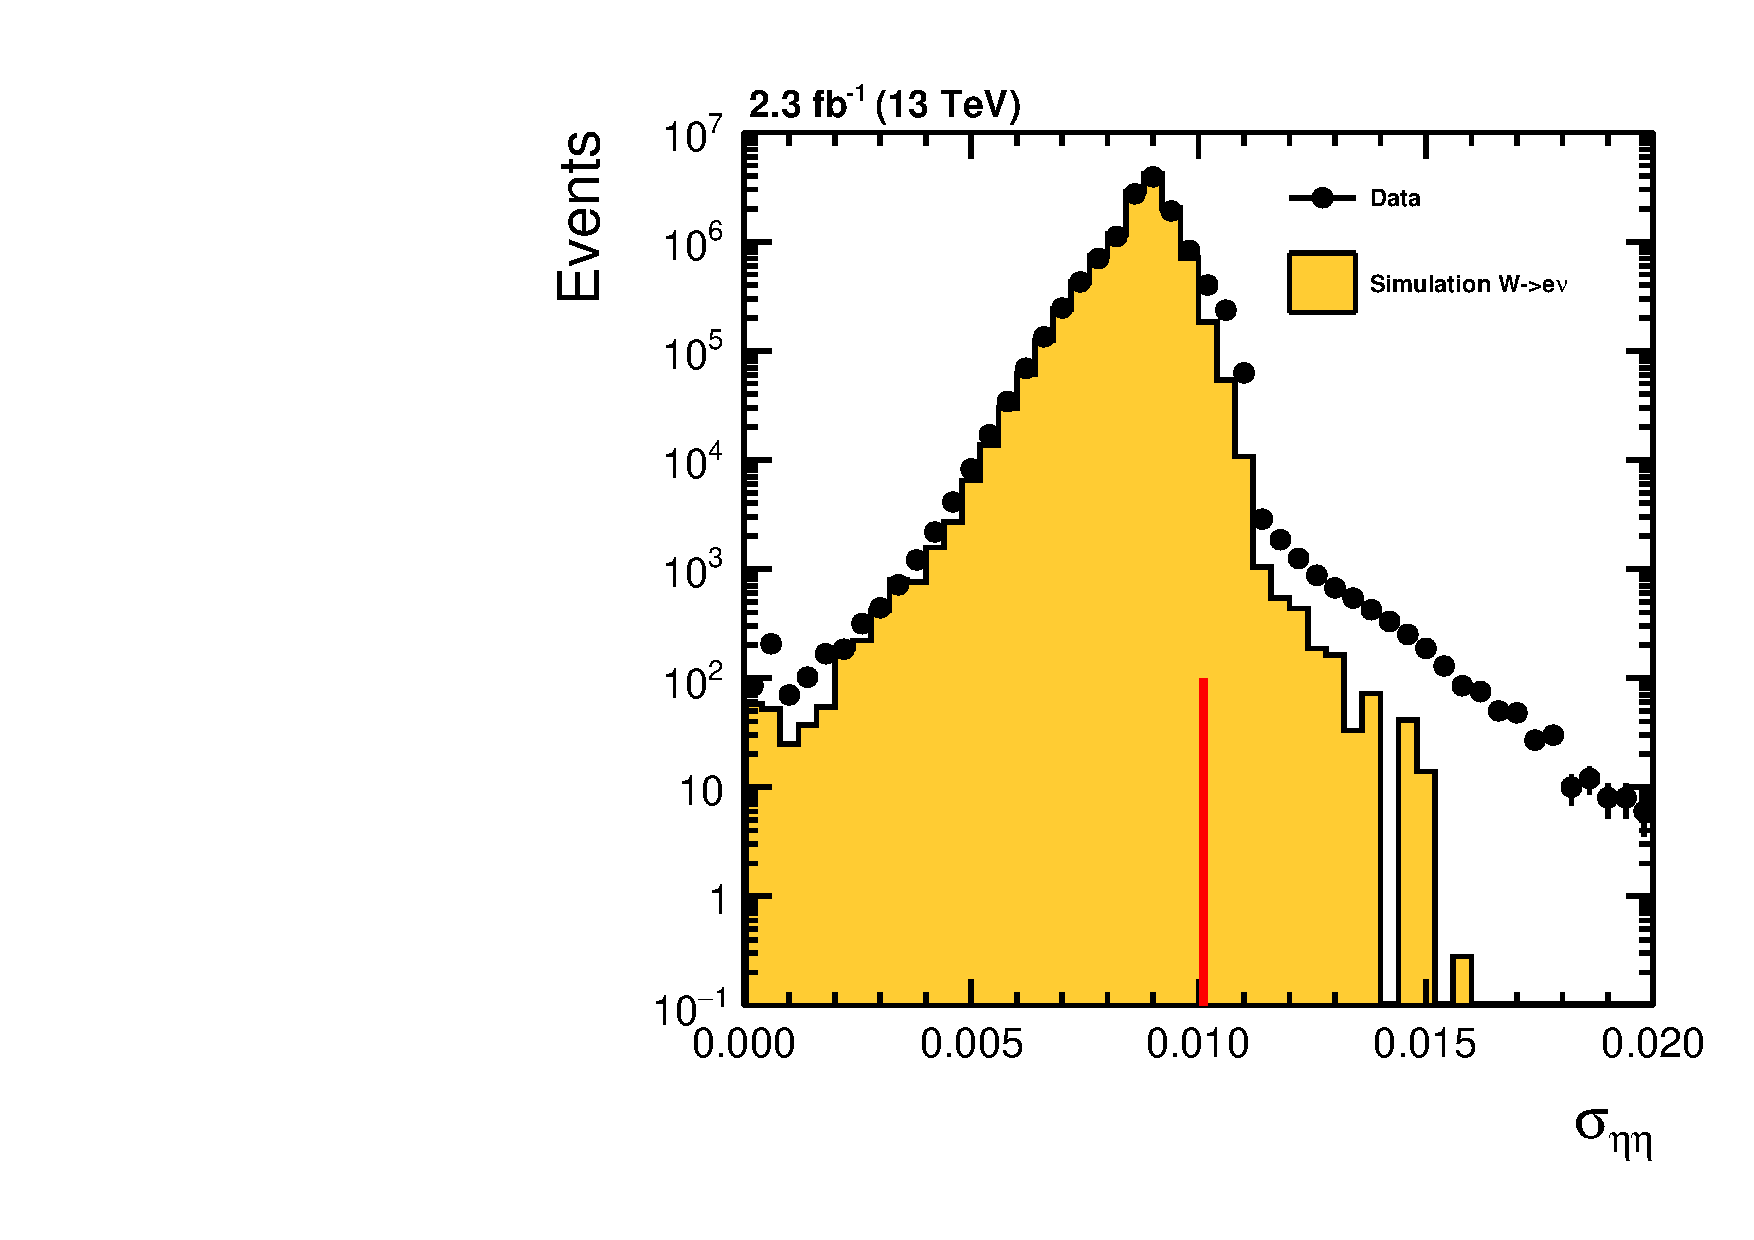
\includegraphics[width=0.44\columnwidth]{figures_chapter4/sigieie_barrel}
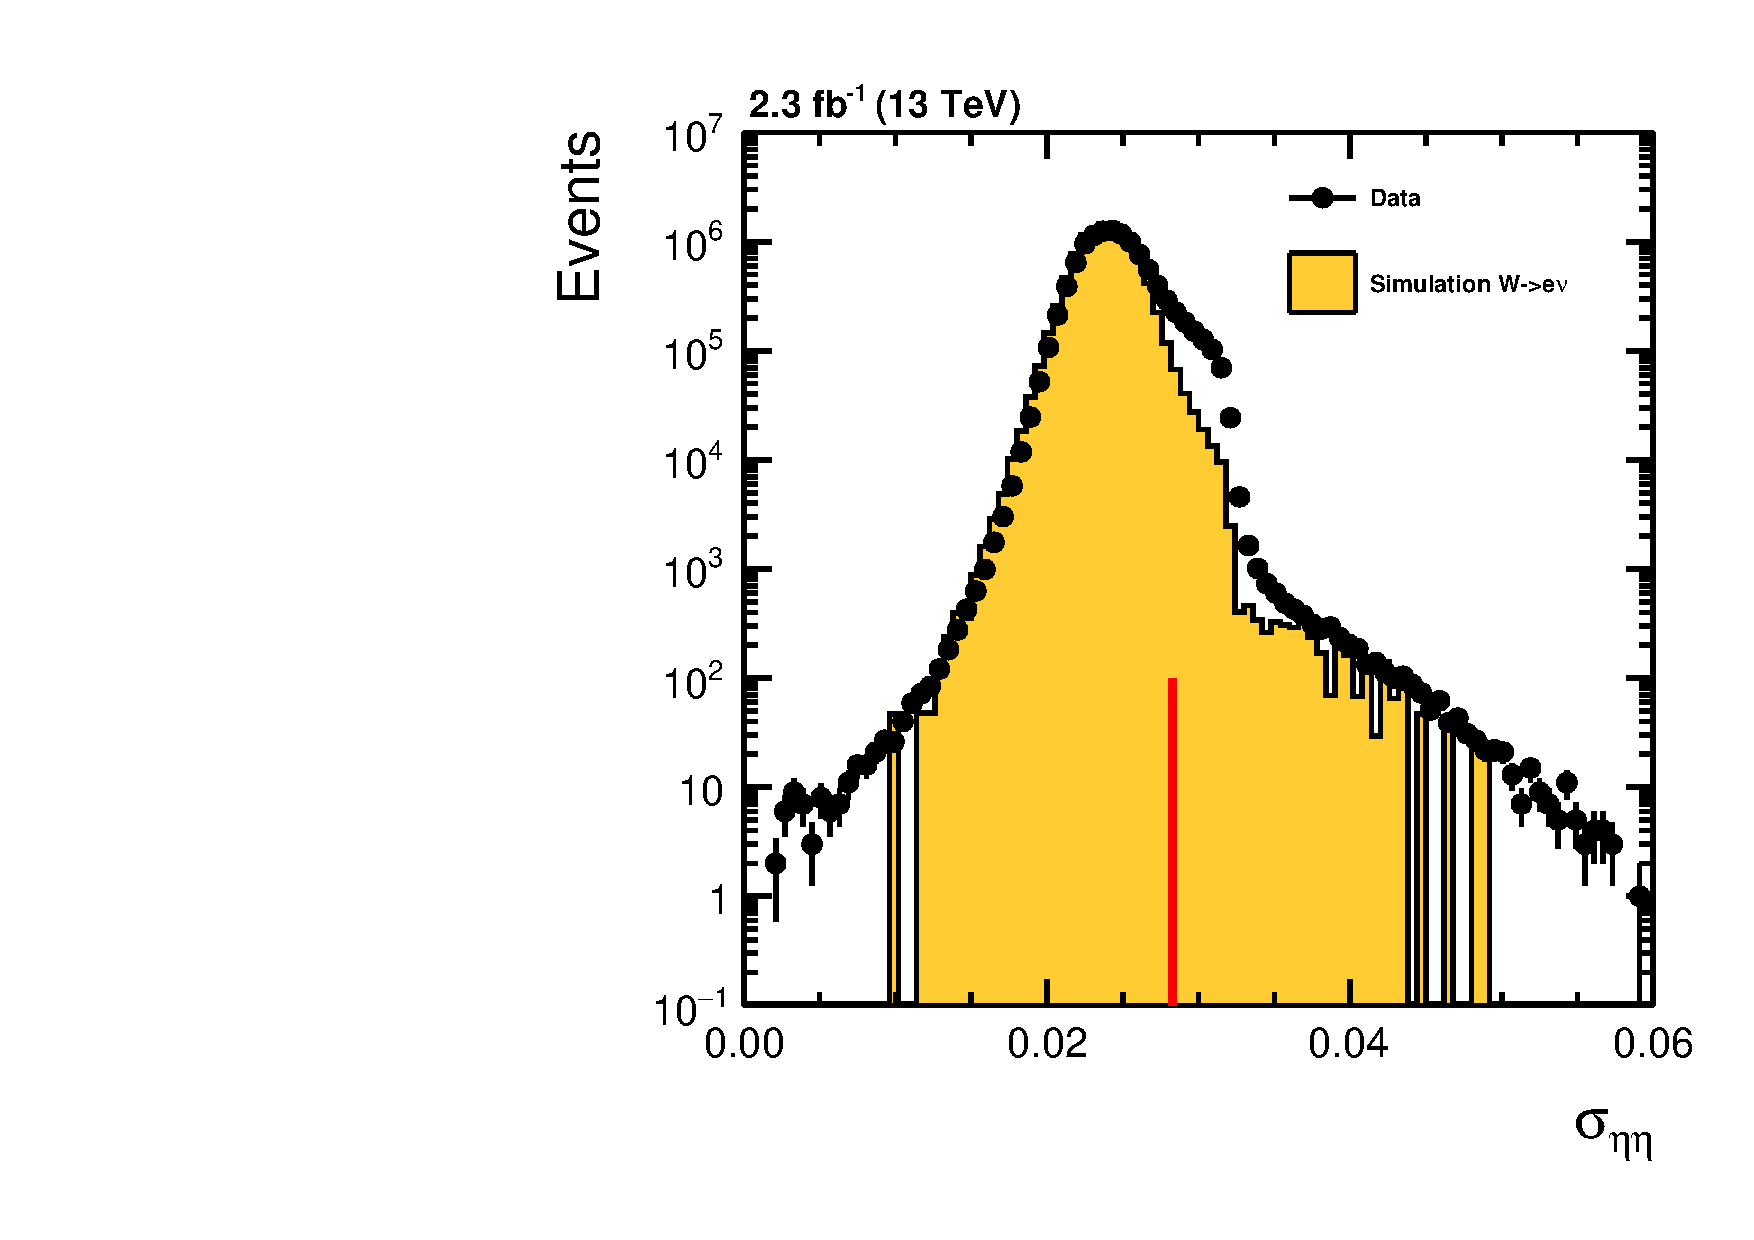
\includegraphics[width=0.44\columnwidth]{figures_chapter4/sigieie_endcap}
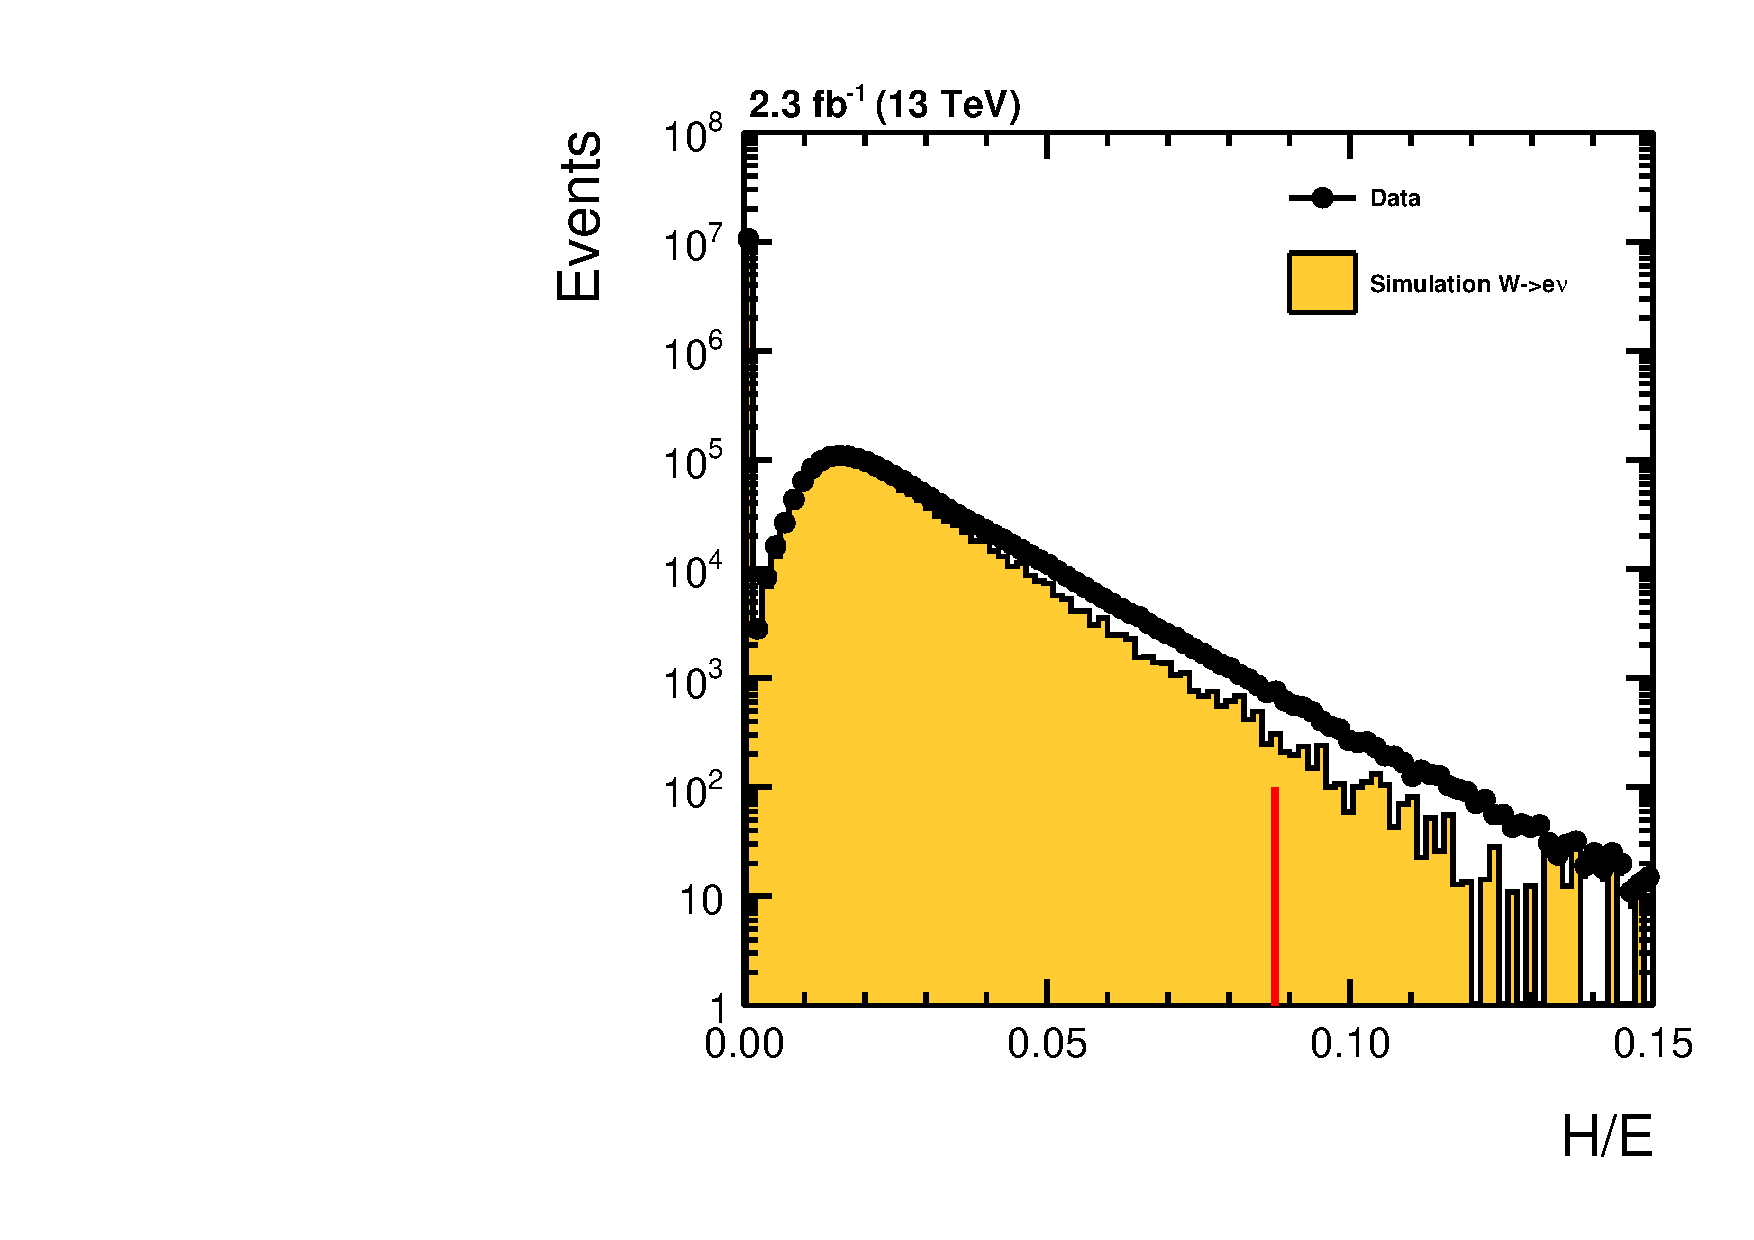
\includegraphics[width=0.44\columnwidth]{figures_chapter4/hovere_barrel}
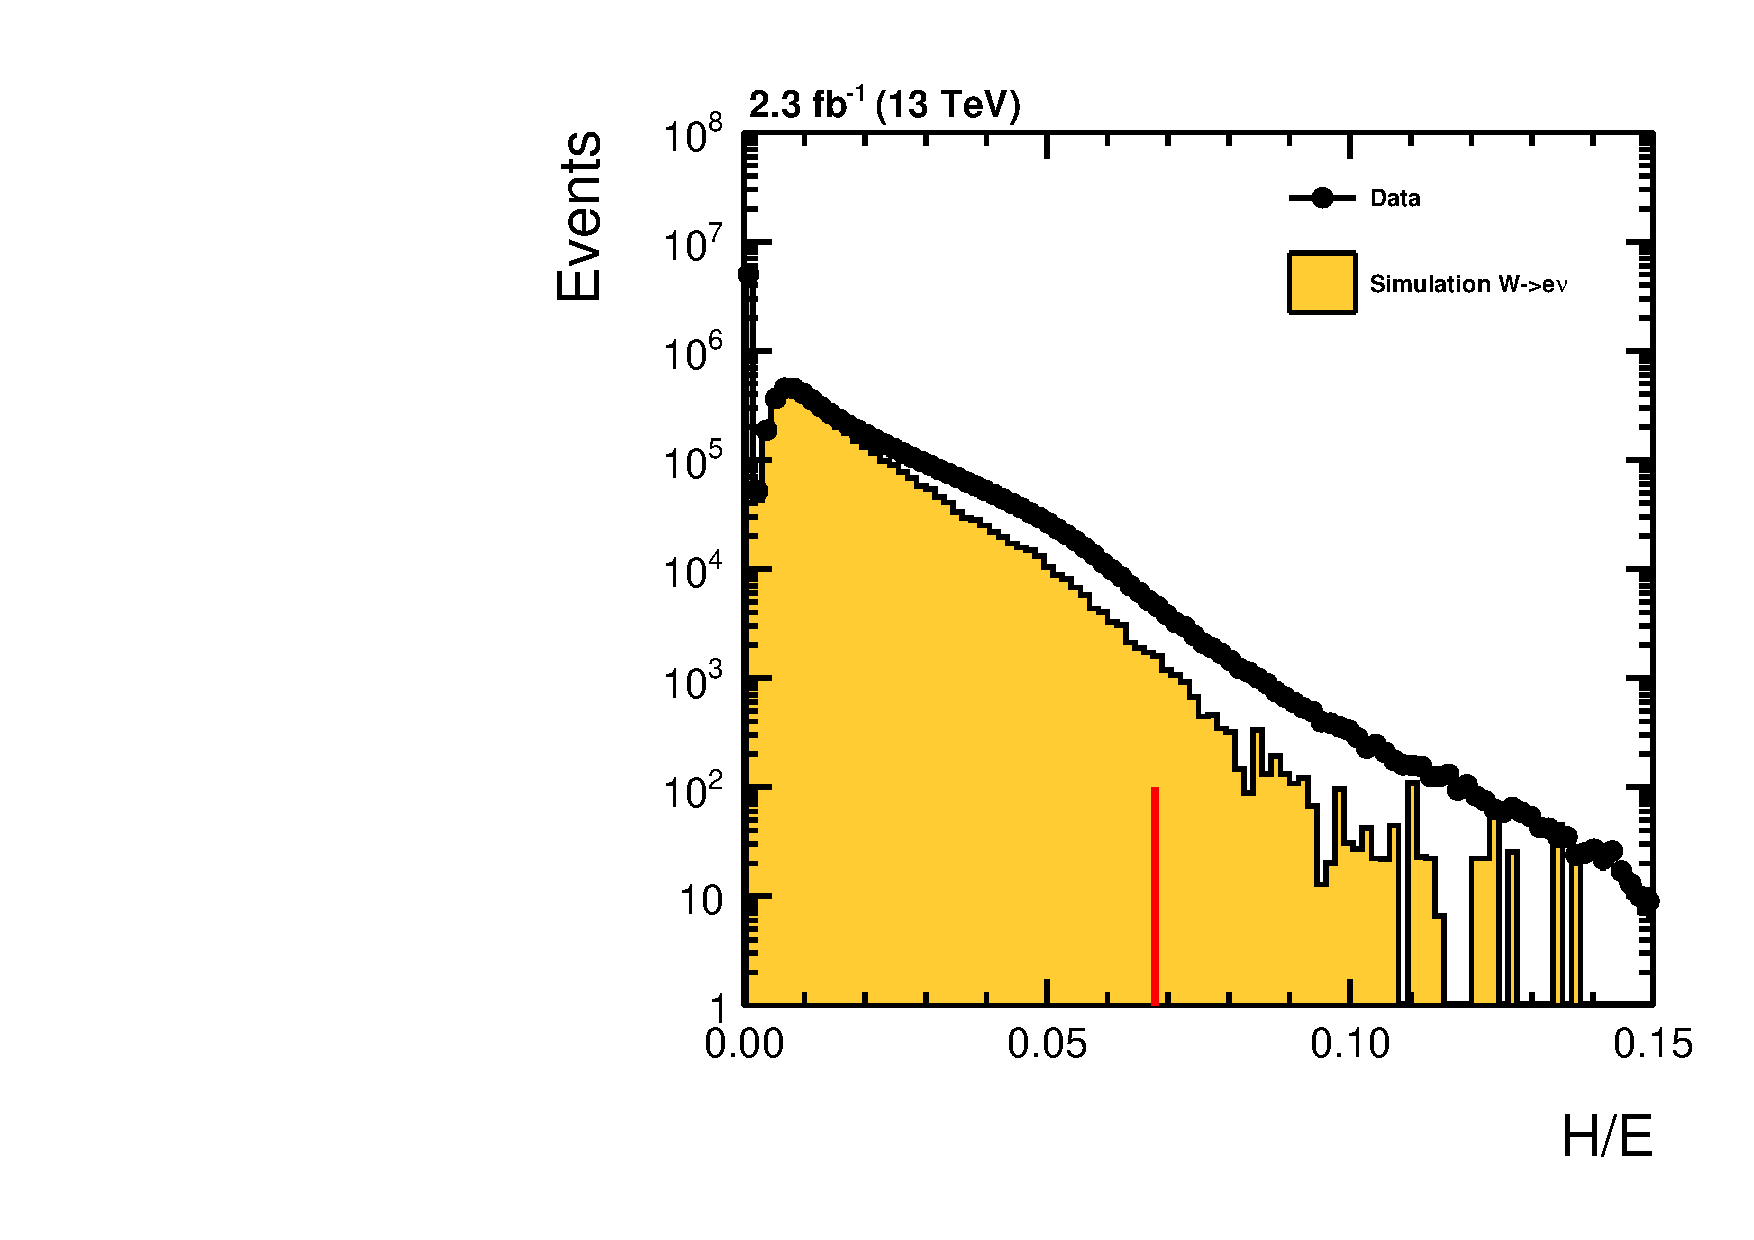
\includegraphics[width=0.44\columnwidth]{figures_chapter4/hovere_endcap}
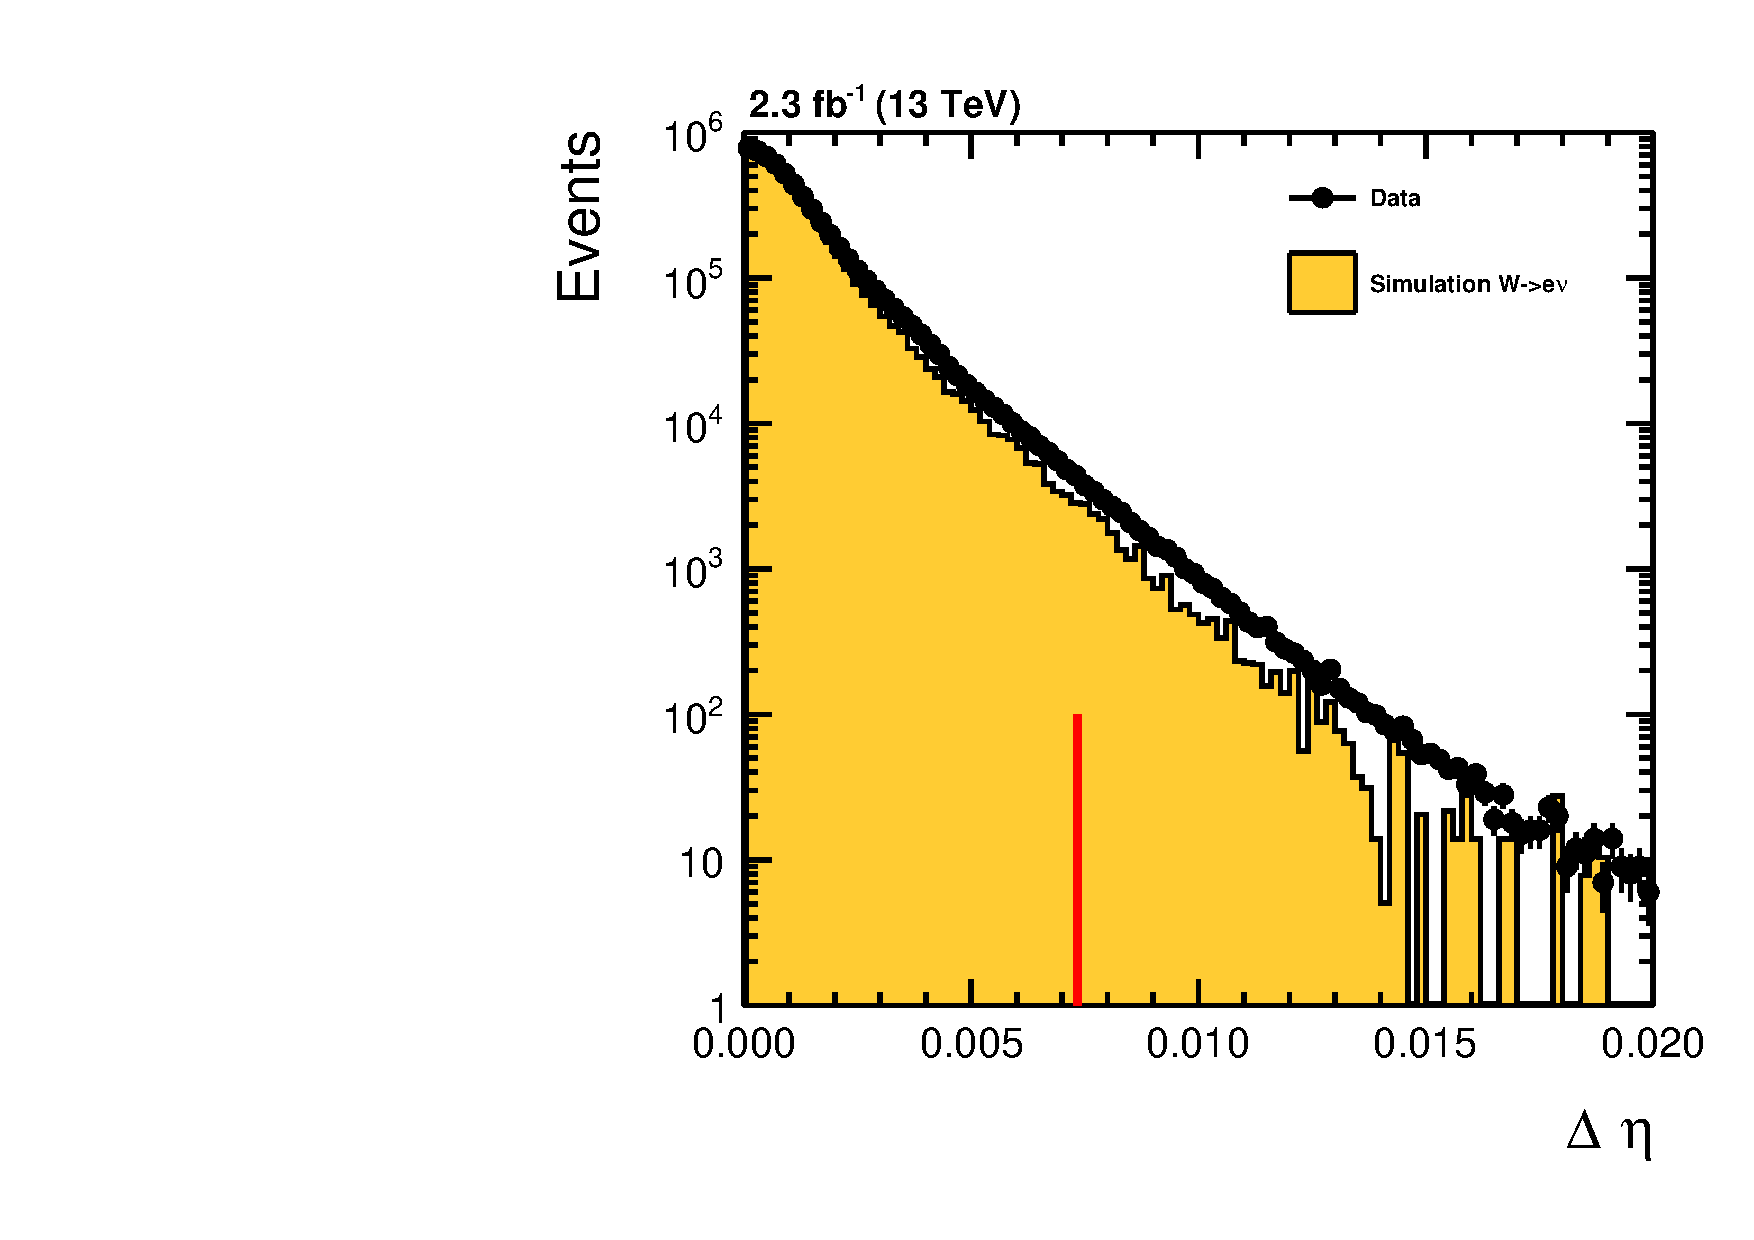
\includegraphics[width=0.44\columnwidth]{figures_chapter4/deta_barrel}
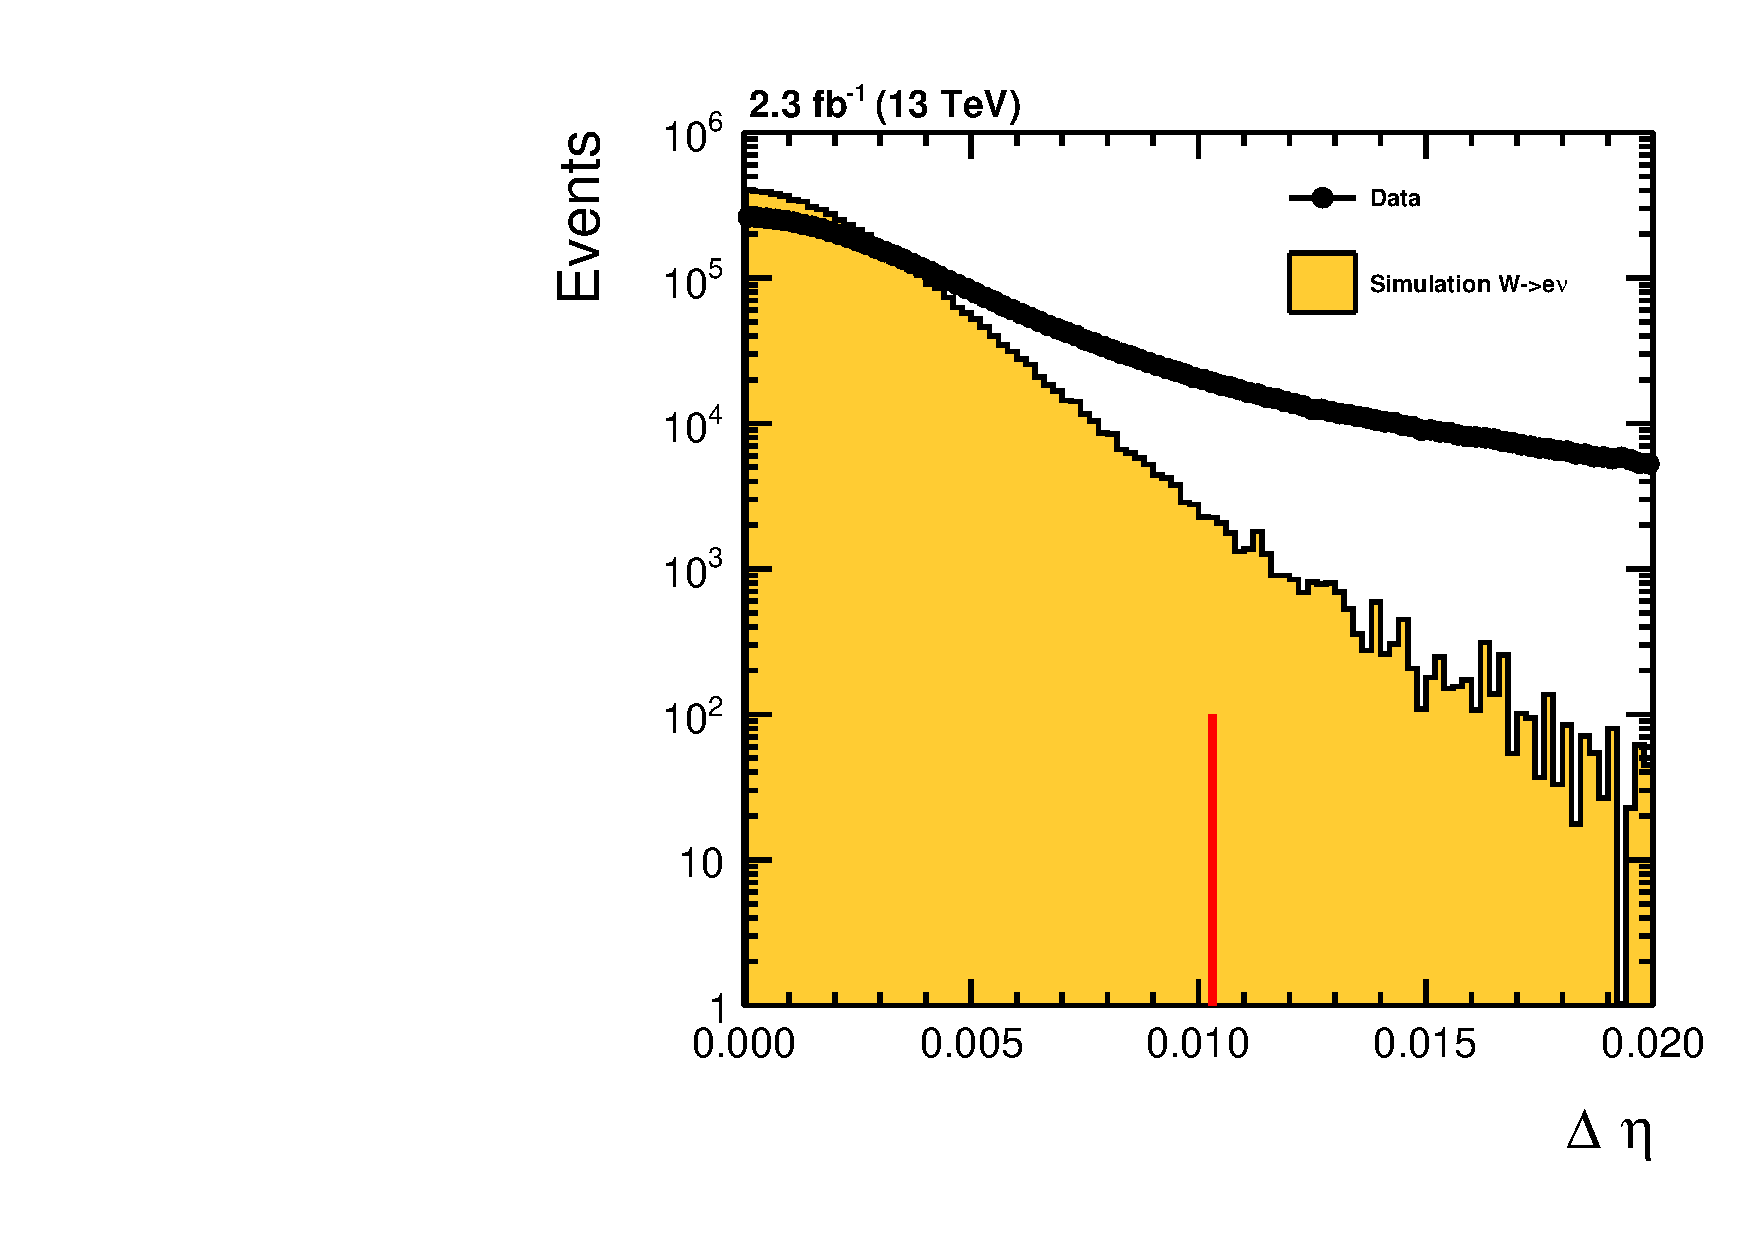
\includegraphics[width=0.44\columnwidth]{figures_chapter4/deta_endcap}
\caption{Distribution of shower shape $\sigma_{\eta \eta}$, H/E, and $\Delta \eta$ for data at $\sqrt{s}=13~\TeV$ taken during $2015$ data taking period for the barrel (left) and endcap (right). Simulated $W \rightarrow e \nu$ signal process normalized to the number of observed data evens is shown for comparison. The events satisfy all other selection requirements (including the isolation requirement to be discussed in Section 3.8) are satisfied except that on the shown variable. The red line illustrates the requirement on the variable for a selection optimized for that data-taking period.}
\label{fig:ele_id}
\end{figure}

In the ECAL barrel region the energy is collected in a small $\eta$ window with an extended window in $\phi$.  An array of $5\times1$ crystals in $\eta-\phi$ are formed around a seed crystal with transverse energy $E_{T}>1~\GeV$. The arrays are extended in both $\phi$ directions centered at the seed crystals up to $\Delta \phi$ of radius of $0.3$. The arrays with $E_{T}>0.1~\GeV$ are grouped to form a supercluster. In the ECAL endcap the supercluster is seeded by a $5\times5$ cluster in $\eta-\phi$ centered at the seed crystal. The supercluster energy corresponds to the sum of the energies of its clusters. 

Inner tracker seeds compatible with a reconstructed supercluster are searched in the pixel tracker (also in TEC to improve the efficiency). Electrons that suffer a small amount of bremsstrahlung radiation loss can be identified by extrapolating a standard reconstructed track to the ECAL and checking if it passes close to an ECAL cluster. On the other hand, a poor $\chi^2$ or few associated hits in the reconstructed tracks may come from an electron that suffered a significant bremsstrahlung energy loss. A modified version of the Kalman filter is used to perform the final fit of the track parameters as the Kalman filter is only optimal for Gaussian uncertainties whereas the bremsstrahlung energy loss is modeled by Bethe-Heitler model.  A gaussian approximation to the Bethe-Heitler model is crude and therefore a Gaussian-Sum filter (GSF)~\cite{Adam:815410} method is employed that approximates the Bethe-Heitler energy loss by a sum of Gaussian functions. The final electron momentum is derived from a weighted mean of the inner tracker measurements and the supercluster energy. 

There are few sources of electron backgrounds. An overlapping charged and neutral pions inside a hadronic jet or a charged pion showering early in the ECAL can be miss-identified as an electrons. Figure~\ref{fig:ele_id} shows the distributions of few of the electron identification variables used for reduction of these background processes:
 
\begin{description}
\item[$\bullet$]  $\sigma_{\eta\eta}$ is the energy weighted $\eta$ width of the cluster. As can be seen it is small for genuine electrons.  
\item[$\bullet$]  H/E is the ratio of the energy deposited in the HCAL to the electromagnetic energy near the seed cluster.
\item[$\bullet$]  $\frac{1}{E}-\frac{1}{p}$ quantifies the energy and momentum compatibility measured in the ECAL and inner tracker respectively.
\item[$\bullet$] $\Delta \eta$ and $\Delta \phi$ are the separations between the supercluster and track directions evaluated at the primary vertex in the $\eta$ and $\phi$ directions respectively.    
\end{description}

The conversion of a photon into an electron-positron pair is another source of background. Electron candidates with missing hits in the innermost layers of the inner tracker indicate a photon conversion. The identification of a vertex with a pair of tracks with no hits in the tracker layers between the vertex and the interaction point is also used to further suppress this background. 

\section{Jet Reconstruction}

Quarks and gluons produced at the LHC fragment and hadronize nearly immediately to a collimated spray of hadrons, known as jets. Jets may originate from a $2 \rightarrow 2$ scattering of the partons inside the colliding protons, decay of a heavy object, such as a top quark or a Higgs boson, and emission of gluons off some other partons in the event. Measuring the jet energy and direction provides information of the original parton. A detailed review of jet finding algorithms, a set of rules for grouping the hadrons into jets, at hadron colliders can be found in~\cite{Salam:2009jx}. So called sequential recombination jet algorithms are used at CMS as implemented in the FastJet package~\cite{Cacciari:2011ma}.  The usual approach of these algorithms is to introduce two distance measures $d_{ij}$ and $d_{iB}$ defined as:
\begin{eqnarray} \label{eq:jet_find}
d_{ij} = min(p_{ti}^{2p},p_{tj}^{2p})\frac{\Delta_{ij}^2}{R^2}, \\
d_{iB} = p_{ti}^{2p},
\end{eqnarray}
where $\Delta_{ij}^2 = (y_{i}-y_{j})^2 + (\phi_{i} -\phi_{j})^2$ and $k_{ti}$, $y_{i}$, and $\phi_{i}$ are the transverse momentum, rapidity, and azimuth of object $i$ in the event. $R$ is the distance parameter and $p$ is the power of the energy scale. From the above definitions it can be seen that $d_{ij}$ and $d_{iB}$ are invariant under a boost along the beam direction. The algorithm proceeds to identify the smallest distance measures in the events. If $d_{ij}$ is the smallest for a given pair of objects, then the two objects are combined into a single object by adding the momenta of the $i$ and $j$ objects. If $d_{iB}$ is the smallest distance then the object $i$ is denoted as a jet and removed from further consideration in the algorithm. The algorithm continues until there are no objects remaining in the event. The anti-$k_{t}$ algorithm~\cite{Cacciari:2008gp} with $p=-1$ is used for the results shown here. A distance parameter of $R=0.5$ or $R=0.4$ is used. The anti-${k_{t}}$ algorithm grows outward from hard "seeds" resulting in a cone-like jets in $\eta-\phi$. The resulting jet boundaries are resilient with respect to soft radiation while the algorithm is infra-red and collinear safe.  


\subsection{Jet Energy Scale}

The jet energy needs to be calibrated to obtain a more accurate estimate of the original parton energy. Corrections are needed to account for the additional energy due to pileup, non-uniformities in the detector response, and detector noise. The effect of additional energy due to pileup and detector noise is corrected on per-jet basis for each event using the median energy density $\rho$ and the jet area~\cite{Cacciari:2007fd}. The pseudorapidity and the jet transverse momentum dependent corrections are derived in simulated events with and without pileup overlay. "Zero-bias" triggered events (from randomly selected non-empty LHC bunch crossings) are used to correct for the residual differences between data and detector simulation.  The average jet energy scale is calibrated using the MC truth in simulation~\cite{1748-0221-6-11-P11002,Khachatryan:2016kdb}. Corrections are then applied to account for residual differences  between the detector simulation and data using the transverse momentum balancing in di-jet, $\gamma$-jet, and $Z$-jet events. The di-jet $p_{T}$ balancing method is used to correct the relative scale using the barrel region $|\eta|<1.3$ as a reference. The absolute scale is corrected using $\gamma$-jet and $Z$-jet events exploiting the excellent $p_{T}$ resolution of photons and leptons. 

\begin{figure}[h]
\centering
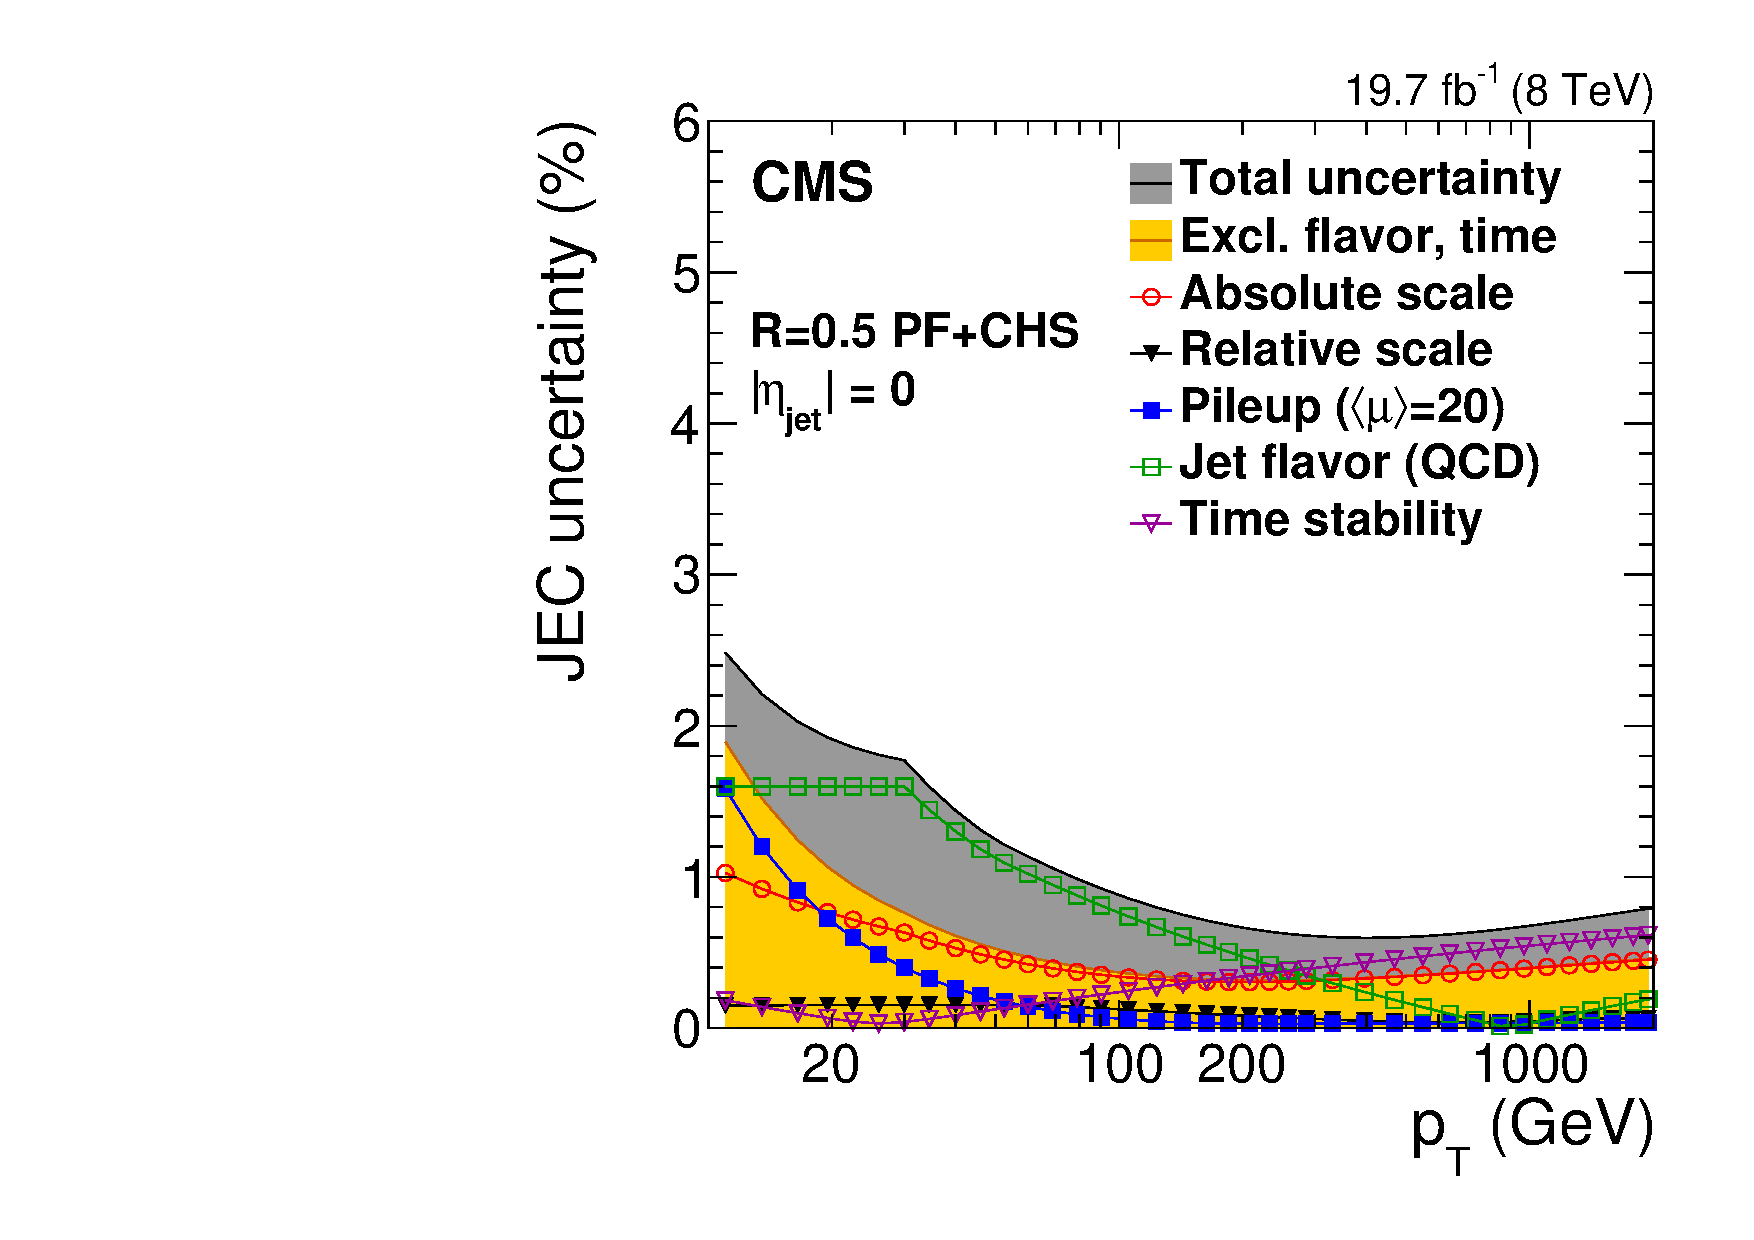
\includegraphics[width=0.49\columnwidth]{figures_chapter4/jec_unc}
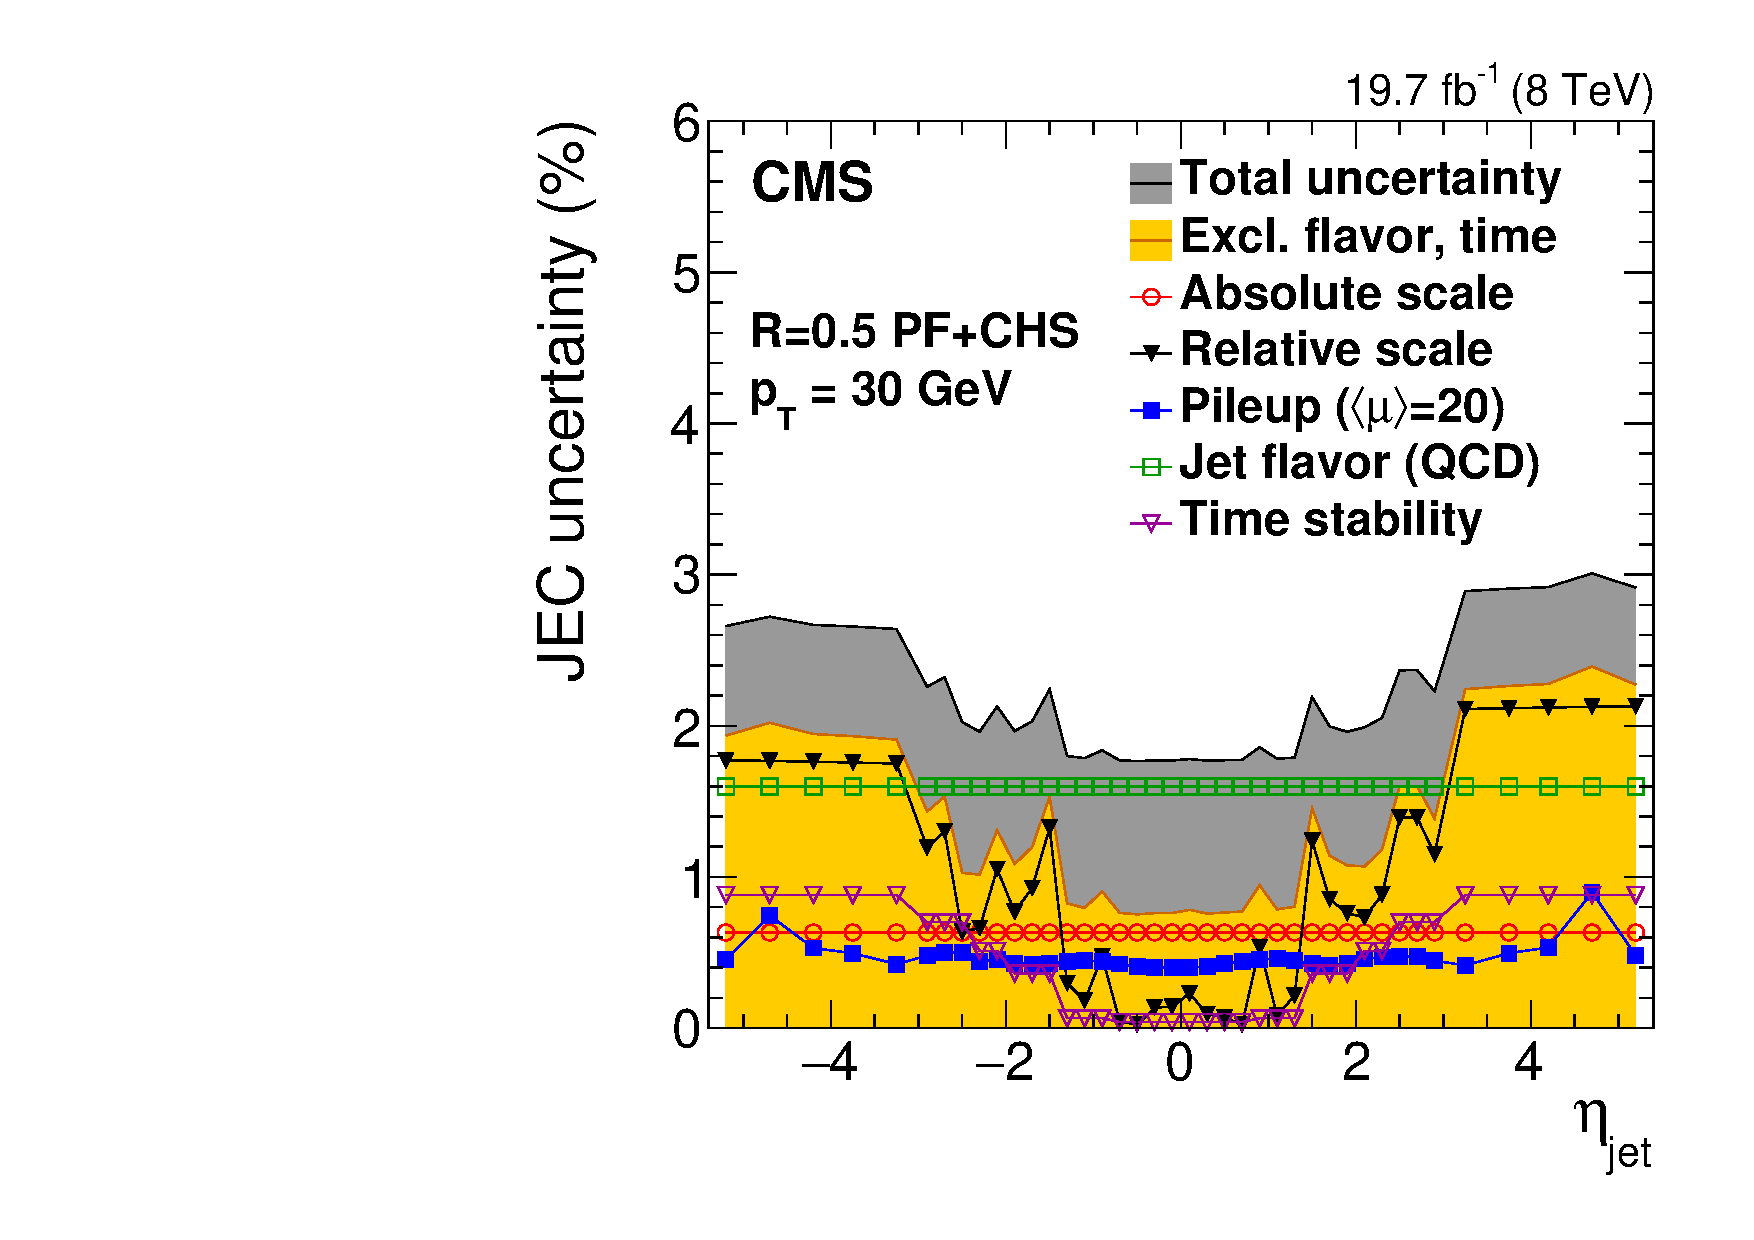
\includegraphics[width=0.49\columnwidth]{figures_chapter4/jec_unc2}
\caption{Summary of jet energy scale systematics as a function of jet $p_{T}$ for $|\eta|=0$ (left) and of jet $\eta$ for $p_{T}=30~\GeV$ at $\sqrt{s}=8~\TeV$ data taking period. The markers show the single effect of different sources and the gray dark band shows the cumulative total uncertainty. The total uncertainty, when excluding the effects of time dependence and flavor, is also shown in yellow light~\cite{Khachatryan:2016kdb}.}
\label{fig:jet_unc}
\end{figure}

Figure~\ref{fig:jet_unc} shows the summary of jet energy scale uncertainties as a function of jet $p_{T}$ and $\eta$ at $\sqrt{s}=8~\TeV$ data taking period. Jets selected for majority of the physics results are required to have a transverse momentum greater than $30~\GeV$ (the $p_{T}$ requirement is lower for jets originating from b quarks) with $|\eta|<4.7$.  The uncertainties on the jet energy scale are below $3\%$ across the phase space considered by most analyses and below $1\%$ in the barrel region when excluding the uncertainties due to jet flavor differences in the events used to derive the different stages of the jet energy scale corrections.

\subsection{Pileup Jet Identification}

The particles originating from pileup interactions can cluster into jets. The $p_{T}$ density due to pileup particles is roughly $0.7~\GeV$ per unit area in $\eta-\phi$ plane for one reconstructed primary vertex. While the pileup jets have low $p_{T}$ it is possible for these low $p_{T}$ jets to overlap and a form a single jet with relatively large $p_{T}$. The number of overlapping jets grows roughly quadratically with the number of pileup interactions and jet area~\cite{CMS-PAS-JME-13-005}.  
The goal of the pileup jet identification algorithm is to mitigate the background events due to the pileup jets. The charged particles in pileup jets generally do not point to the primary vertex of the event. In addition, jets originating from pileup tend to be more diffuse in shape compared to the jets from the hard scattering. These two characteristic signatures of the pileup jets are exploited. A Boosted Decision Tree (BDT) discriminant implemented in TMVA~\cite{H�cker:1019880} is used. It takes as an input the compatibility of the tracks inside the jet with the primary vertex of the event, variables exploiting the jet shape, and the number of charged and neutral constituents of the jet. The most discriminating track related variable ($\beta^{*}$) and jet shape variable ($<\Delta R^2>$) are defined as:
\begin{eqnarray} \label{eq:pujetid}
\beta^{*} = \frac{\sum_{i \notin \mathrm{PV}} p_{Ti}}{\sum_{i} p_{Ti}}, \\
<\Delta R^{2}> = \frac{\sum_{i \in \mathrm{jet}} \Delta R^{2} p_{Ti}^2 }{\sum_{i \in jet} p_{Ti}^2},
\end{eqnarray}
where the charged particle is defined to be coming from the primary vertex if $\Delta z<0.2$ cm in the $\beta^{*}$ definition and $\Delta R$ is the distance of the particle to the jet axis in the $<\Delta R^{2}>$ definition. The distributions of these variables for "real" and pileup jets are shown in Figure~\ref{fig:pu_jet}. The $<\Delta R^{2}>$ distributions are shown for jets with $|\eta|>3.0$ where there is a degradation of separation due to the coarse granularity of the HF calorimeter. 

\begin{figure}[h]
\centering
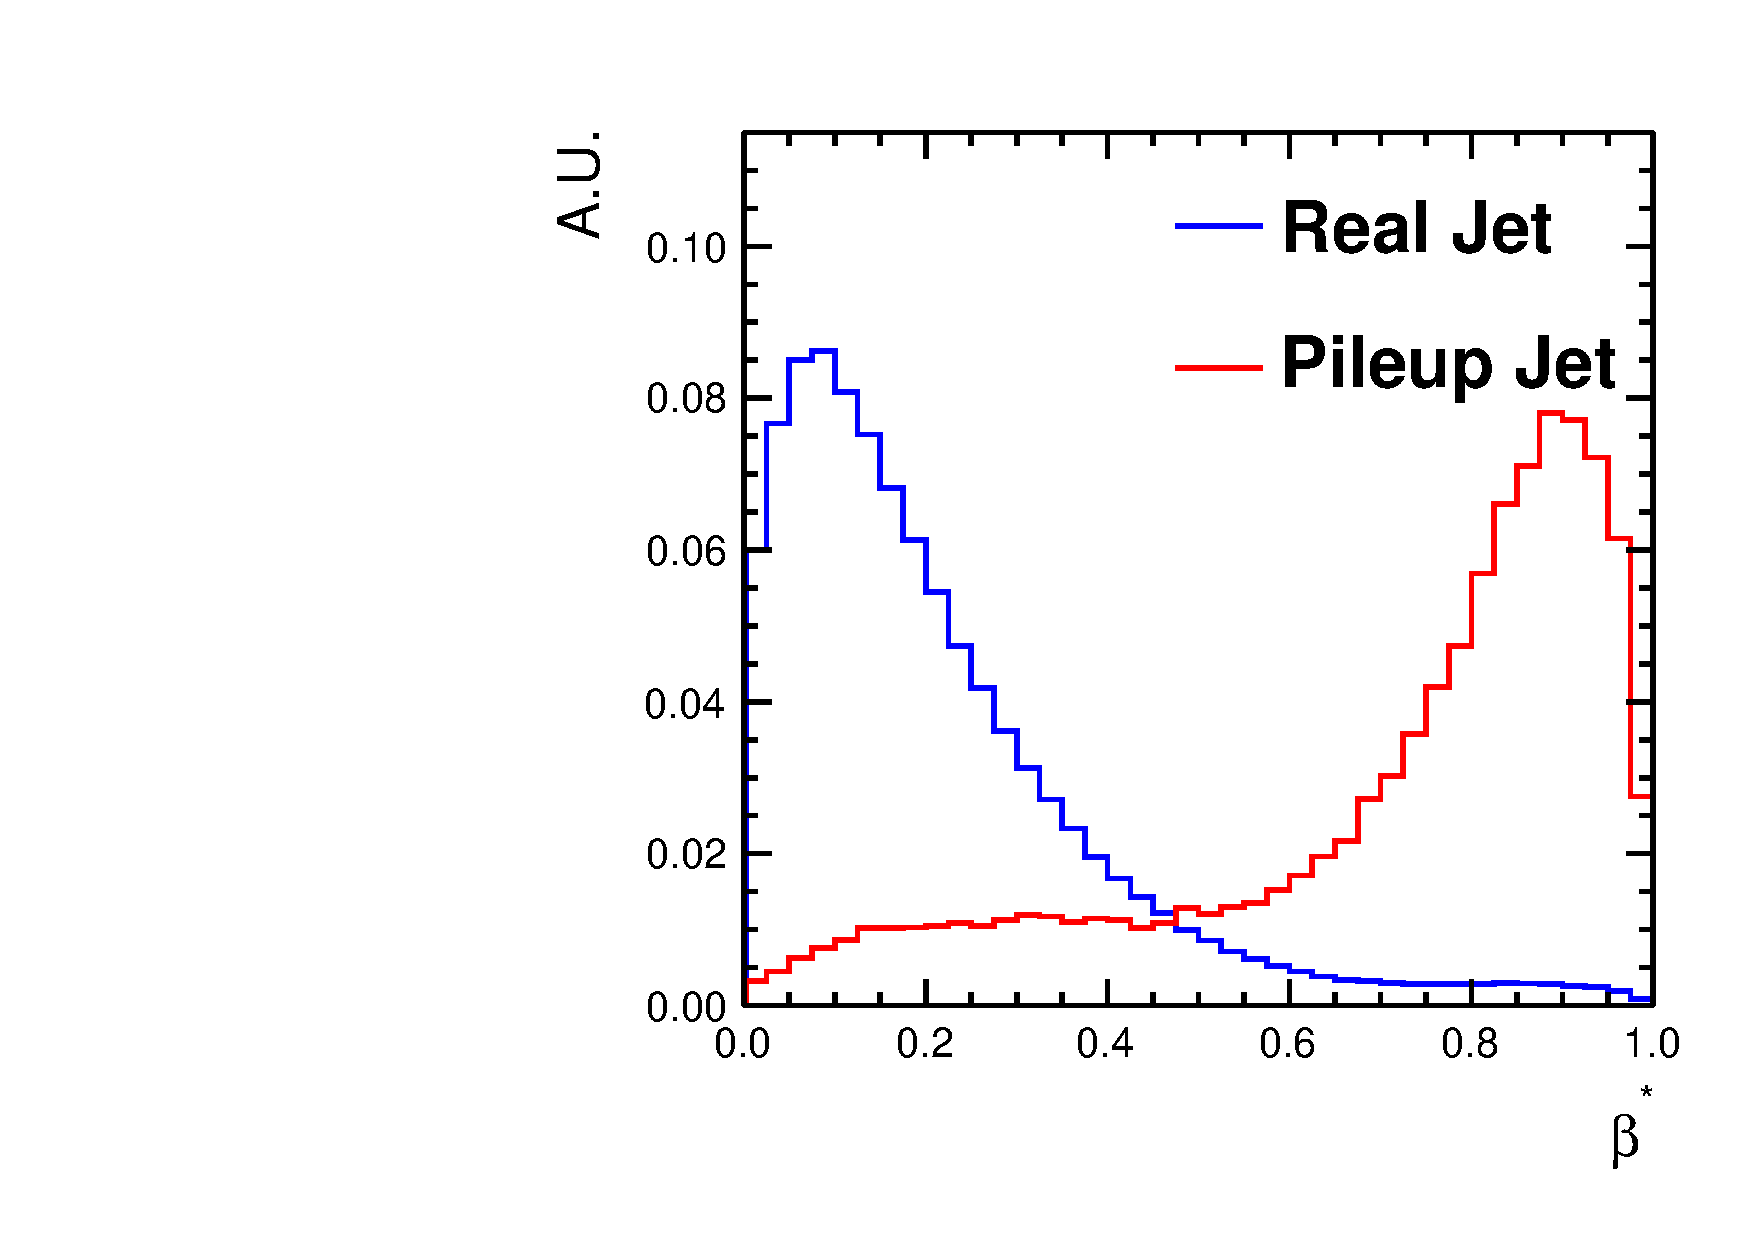
\includegraphics[width=0.49\columnwidth]{figures_chapter4/bstar}
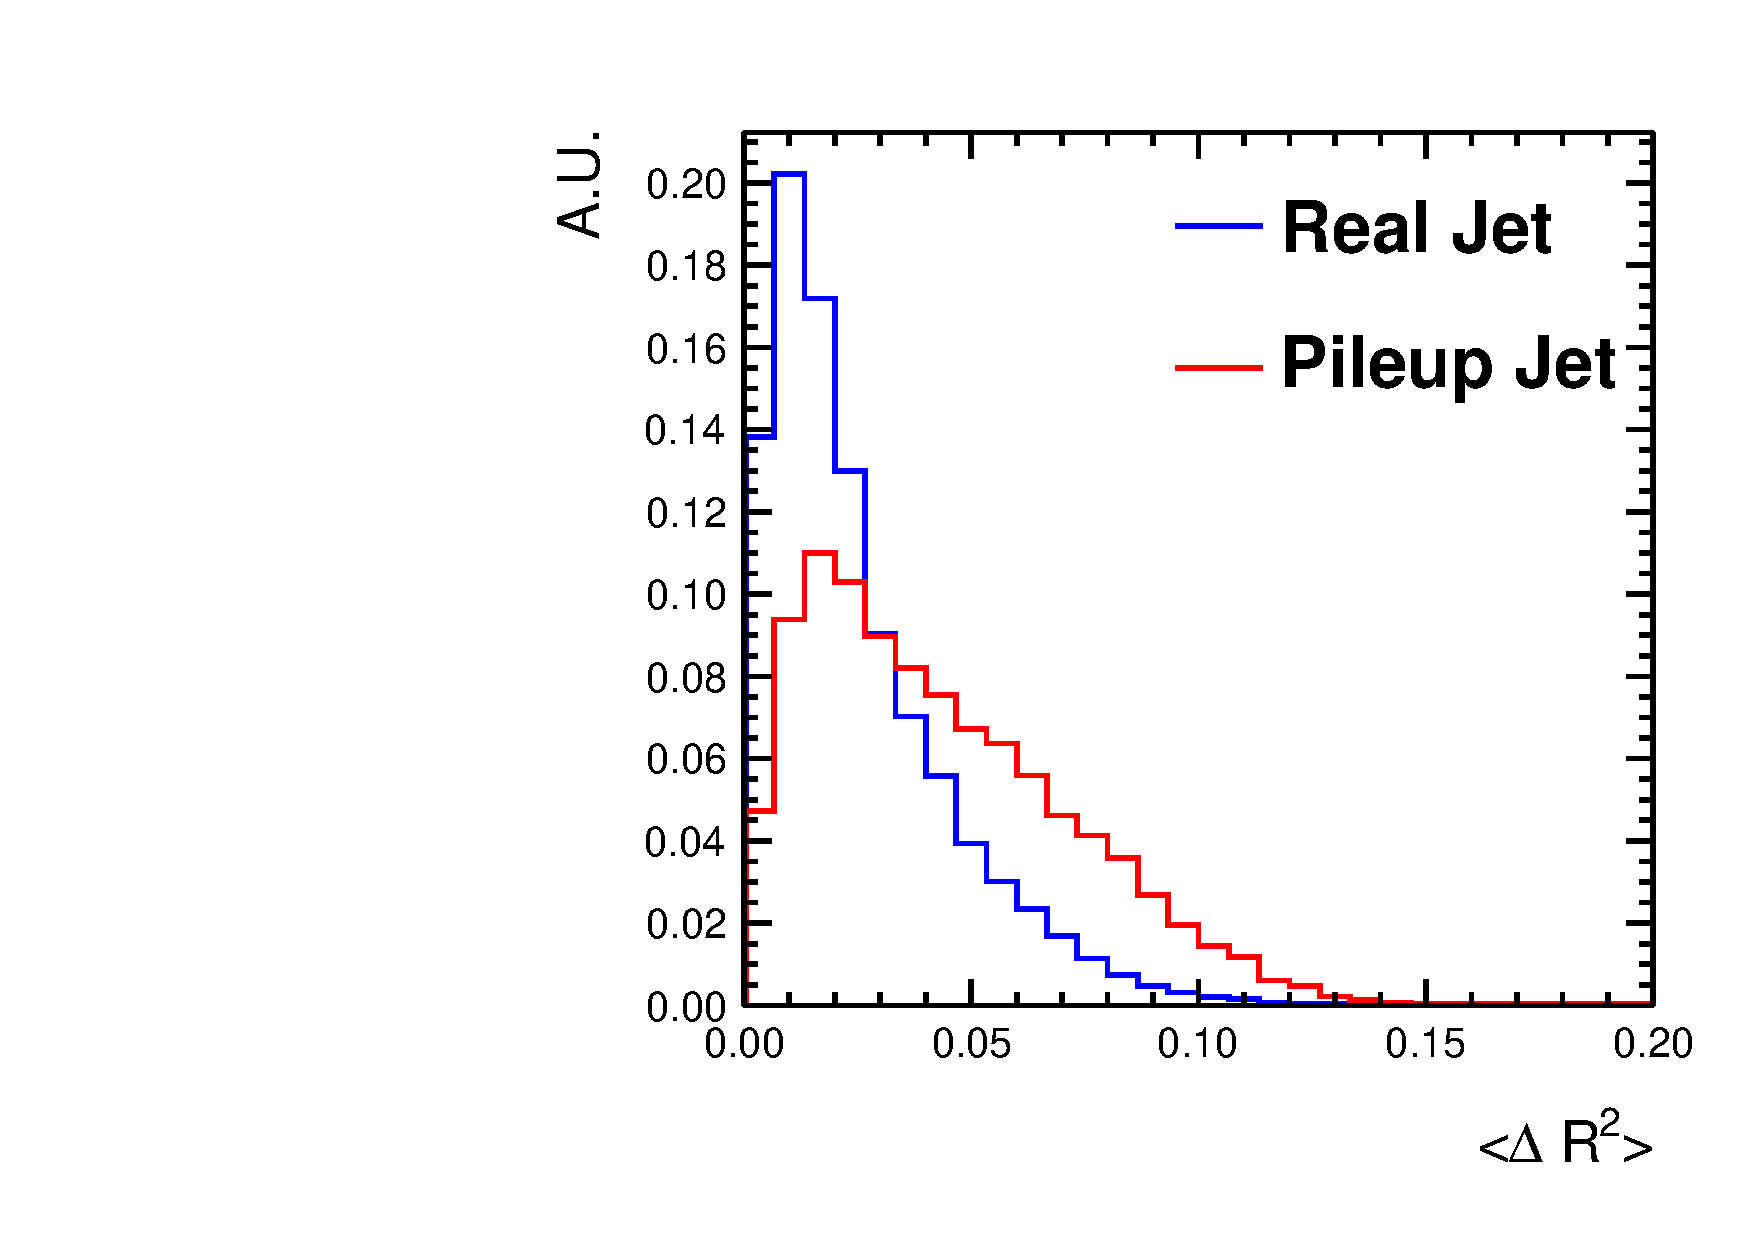
\includegraphics[width=0.49\columnwidth]{figures_chapter4/dr2}
\caption{Distributions of the $\beta^{*}$ (left panel) and $<\Delta R^{2}>$ (right panel) variables in simulation for jets matched to MC truth jet within a radius of $\Delta R<0.25$ (blue) and for jets with no match (red). Jets are required to have a $p_{T}$ greater than $25~\GeV$ and $|\eta|<2.5$ (left), and $|\eta|>3.0$ (right).}
\label{fig:pu_jet}
\end{figure}

The BDT discriminator is almost fully efficient for jets with $p_{T}>30\GeV$ in the inner tracker geometric acceptance ($|\eta|<2.4$) region with a pileup jet rejection rate of approximately $87\%$. The efficiency degrades outside of the inner tracker volume. It is about $90\%$ for "real" jets with a pileup jet rejection rate of about $40\%$ for jets with $3.0<|\eta|<5.0$.

\subsection{b-jet Identification}

The identification of jets originating from bottom quark hadronization (b-jet) is crucial to reduce the overwhelming background from processes involving jets originating from gluons, light flavored quarks, and charm quarks (c-jets).  b-jets are important signatures to study the top quark decays, the Higgs boson, and in searches for new physics. The main idea is to exploit the long lifetimes of the bottom and charm quarks and their relatively large mass. As a result, one can look for secondary vertices and/or tracks with large impact parameters.  For example, the CMS inner tracking detector allows to achieve an impact parameter resolution of about $15$ ($30$) $\mu$m for a track with $p_{T}$ of $100$ ($5$)~$\GeV$ while typical impact parameter values for tracks from the b-jets are at a level of a few $100$ $\mu$m~\cite{Chatrchyan:2012jua}. The so called Combined Secondary Vertex (CSV) algorithm~\cite{Chatrchyan:2012jua} is used to identify the b-jets. A likelihood discriminant is formed combining information about track impact parameters and secondary vertices. This means that the b-jets can only be identified within the inner tracker geometrical acceptance ($|\eta|<2.4$). A b-jet identification efficiency of about $75\%$ is achieved with a light-flavor jet miss-identification rate of about $1\%$. 

\section{Particle Flow}

CMS uses the so called particle flow (PF) approach to calorimetry~\cite{CMS-PAS-PFT-09-001,CMS-PAS-PFT-10-001,CMS-PAS-PFT-10-002}.  The basic idea of the PF approach is to combine information from all sub-detectors in order to reconstruct all the particles in the event using the best measurements possible. This is especially useful for jet energy measurements as roughly $62\%$ of the jet energy is carried by charged particles (mainly hadrons), around $27\%$ by photons, about $10\%$ by long lived neutral hadrons, and around $1.5\%$ by neutrinos~\cite{Thomson200925}. Thus, one can exploit the superior momentum (energy) resolution of the inner tracker (ECAL) to obtain the most accurate measurements for the charged hadrons (photons) inside the jet and within the inner tracker (ECAL) geometric acceptance. In addition, the high granularity ECAL makes it possible to separate photons from charged particle energy deposits. 

 The basic elements of the PF algorithm are tracks in the inner tracker, muon segments in the muon system, and energy clusters from the calorimeters. The calorimeter clustering allows to separate the neutral particles from the energy deposits of charged hadrons as well as to reconstruct and identify the electrons and the corresponding bremsstrahlung photons. The clustering starts from the cluster seed defined as a local energy maxima. The clusters are then grown from the seeds by including neighboring cells, with an energy in excess of a defined threshold, in the cluster. The threshold is defined to be two standard deviation of the electronic noise of the ECAL ($80~\MeV$ in the barrel and  approximately $300~\MeV$ in the endcap) and $800~\MeV$ in the HCAL. A linking algorithm is required as a given particle will result in several PF elements. This is achieved by defining a distance measure between each pair of PF elements. For example, the ECAL clusters of bremsstrahlung photons emitted by an electron are linked by extrapolating the tangents of the track at each intersection point with an inner tracking detector layer to the ECAL to form a PF block. It has to be noted that due to high granularity of the CMS detector the linked blocks typically contain only $1-3$ elements. The PF candidates are identified from these blocks. 
 
 The block and the corresponding PF elements are iteratively removed from further consideration once a PF candidate has been identified. A global muon is denoted as a PF muon if a track element is compatible with the global muon. The track is removed from further consideration and the expected energy deposits in the calorimeters are subtracted from the corresponding calorimeter clusters.  The GSF electron tracks are linked to the ECAL clusters using a discriminator against charged pions that utilizes information from the inner tracker and the ECAL. A PF electron is formed from the GSF tracks and the ECAL clusters (including the clusters identified as bremsstrahlung photons) in case of a positive match. The remaining inner tracker tracks are identified as charged hadrons. If the linked calorimeter cluster energy exceeds the tracker momentum (taking the relevant measurement uncertainties into account), the corresponding energy excess is identified as a neutral particle. In addition, a PF photon is identified if the excess energy is larger than the linked ECAL cluster while the remaining energy is assigned to a neutral hadron. The remaining ECAL (HCAL) clusters that do not have a linked track are denoted as PF photons (PF neutral hadrons).   
 
 The output of the PF algorithm are denoted as particle flow candidates and are classified as electrons, photons, muons, charged hadrons, or neutral hadrons. The particle flow candidates are used for the reconstruction of jets (referred as PF jets) described in the previous section. A special version of the PF algorithm is used in the HLT optimized to the HLT requirements. 

\section{Hadronic Tau Decays}

The $\tau$ lepton with a mass of $1.777~\GeV$~\cite{Agashe:2014kda} is the only lepton sufficiently heavy to be able to decay to hadrons.  Hadronic tau decays proceed via weak interaction into one or three charged pions or kaons with up to two neutral pions, and one tau neutrino ($\nu_{\tau}$). The $\nu_{\tau}$ escapes the detector resulting in a missing energy in the event. The $\pi_{0}$ meson decays almost exclusively to a pair of photons. Table~\ref{tab:tau_decay} summarizes the most common hadronic tau decays. The mean lifetime of the $\tau$ lepton is $2.9\times10^{-13}$ s~\cite{Agashe:2014kda} resulting in a significant (compared to the transverse impact parameter and secondary vertex resolution) displacement of the decay vertex from the production vertex for energetic taus. The hadronic tau decays are denoted as $\tau_{h}$ henceforth. The tau decays to muons and electrons are denoted as $\tau_{\mu}$ and $\tau_{e}$ respectively.  

\begin{table}[htbp]
\begin{center}
\begin{tabular}{lcc} 
\hline 
Decay Mode & Resonance  & Branching fraction $[\%]$   \\ 
\hline 
$\tau^{\pm} -> h^{\pm} \nu_{\tau}$                             &             & 11.5 \\
$\tau^{\pm} -> h^{\pm} \pi^{0} \nu_{\tau}$                    & $\rho(770)$ & 26.0 \\
$\tau^{\pm} -> h^{\pm} \pi^{0}  \pi^{0} \nu_{\tau}$            & $a_1(1260)$            & 10.8 \\
$\tau^{\pm} -> h^{\pm} h^{\pm} h^{\mp} \nu_{\tau} $            & $a_1(1260)$            & 9.8 \\
$\tau^{\pm} -> h^{\pm} h^{\pm} h^{\mp} \pi^{0} \nu_{\tau} $ &                         & 4.8 \\
Other hadronic modes &                         & 1.8 \\ 
\hline 
All hadronic modes &                         & 64.8 \\ 
\hline 
\end{tabular}
\caption{Approximate branching fractions of hadronic tau decay modes~\cite{Agashe:2014kda}. The intermediate meson resonances are indicated where appropriate. The symbol $h$ represents a charged pion or kaon.
}
\label{tab:tau_decay}
\end{center}
\end{table}

The visible decay products in the $\tau_{h}$ decays result in collimated jets with a relatively low particle multiplicity. The main idea of the $\tau_{h}$ reconstruction algorithm is to reconstruct the individual decay modes listed in Table~\ref{tab:tau_decay}. The hadron-plus-strip (HPS) algorithm~\cite{1748-0221-7-01-P01001} takes advantage of the PF algorithm using the reconstructed charged and neutral PF candidates.  The HPS algorithm starts with a PF jet of $p_{T}$ greater than $14~\GeV$ and $|\eta|<2.5$ using the anti-$k_{T}$ algorithm with distance parameter of $R=0.5$. The photons produced in $\pi^{0} \rightarrow \gamma\gamma$ decays are likely to convert to an electron-positron pair within the volume of the inner tracker. This is taken into account by clustering the electrons and photons (with $p_{T}>0.5~\GeV$)  in the jet into strips in the $\eta-\phi$ plane with a window size of $0.05\times0.20$ taking the direction of the bending of the charged trajectories into account. Strips with total $p_{T}$ sum larger than $2.5~\GeV$ are identified as $\pi^{0}$ candidates. 

$\tau_{h}$ candidates are formed by combining the clustered strips with the charged candidate constituents of the jets. The charged particles are required to have a $p_{T}$ greater than $0.5~\GeV$. The distance of closest approach to the charged particle of highest $p_{T}$ in the jet has to be less than $0.4$ cm in the $z$ direction and $0.03$ cm in the transverse plane~\cite{1748-0221-11-01-P01019}. The following decay hypotheses are considered:

\begin{description}
\item[$\bullet$ $h^{\pm}$:] A single charged particle with no $\pi^{0}$ candidates.  
\item[$\bullet$ $h^{\pm} \pi^{0}$:] One charged particle and one strip with a system mass of $0.3<m_{\tau_{h}}<1.3~\GeV$ for $p_{T}<200~\GeV$. The size of the mass window is enlarged for $\tau_{h}$ candidates with high $p_{T}$ to account for the inner tracker momentum resolution degradation. The mass cut utilizes the intermediate meson resonance ($\rho(770)$) mass in the decay. 
\item[$\bullet$ $h^{\pm} \pi^{0}  \pi^{0}$:] One charged particle combined with two strips. The mass cut requirement is $0.4<m_{\tau_{h}}<1.2~\GeV$ for $p_{T}<200~\GeV$ targeting the intermediate meson resonance decay of $a_{1} (1260)$.  The size of the mass window is enlarged for $\tau_{h}$ candidates with high $p_{T}$.
\item[$\bullet$ $h^{\pm} h^{\pm} h^{\mp}$:] A combination of three charged particles with a system mass of $0.8<m_{\tau_{h}
}<1.5~\GeV$. The sum of the charges is required to be $1$. The charged tracks are required to originate from the same event vertex ($\Delta z< 4$ mm).
\end{description}

\begin{figure}[h]
\centering
\includegraphics[width=0.80\columnwidth]{figures_chapter4/tau_mass}
\caption{Distribution of the $\tau_{h}$ masses in $Z/\gamma^{*} \rightarrow \tau\tau$ events selected in data during $\sqrt{s}=8~\TeV$ data taking period. Expected predictions from the simulation are also shown. The $Z \rightarrow \tau\tau$ prediction is split into the different expected $\tau_{h}$ decay modes. The electroweak background is mainly due to $W+$jets production~\cite{1748-0221-11-01-P01019}.}
\label{fig:tau_mass}
\end{figure}

An additional requirement is imposed on the separation of the charged hadrons and strips. All the charged hadrons and strips are required to be within a narrow cone of $\Delta R = 3.0 /p _{T}~[\GeV]$ around the jet axis to exploit the collimation of the decay products of energetic taus. When $\Delta R$ is smaller than $0.05$ or exceeds $0.10$, a cone size of $0.05$ or $0.10$ is used respectively. Figure~\ref{fig:tau_mass} shows the distribution of the mass of $\tau_{h}$ for $Z/\gamma^{*} \rightarrow \tau\tau$ events at $\sqrt{s}=8~\TeV$ data taking period. The individual decay modes are highlighted by splitting the simulated $Z/\gamma^{*} \rightarrow \tau\tau$ events according to the reconstructed $\tau_{h}$ decay mode. As one can see the $m_{\tau_h}$ distribution peaks around the intermediate meson resonance masses of $\rho(770)$ and $a_{1}(1260)$. The narrow peak near the charged pion mass is due to the single charged particle decay mode. 

Jets originating from quarks and gluons remain a large background to the $\tau_{h}$ reconstruction. This background is further reduced by requiring the selected $\tau_{h}$ candidates to be isolated. The $\tau_{h}$ candidate isolation is discussed in the next section. It is also possible for an electron or muon to be miss-identified as a $\tau_{h}$ candidate. For example, an electron with a radiated bremsstrahlung photon that undergoes a pair conversion is likely to be reconstructed as a $h^{\pm} \pi^{0}$ decay mode.  Miss-identified muons are rejected if track segments are found in at least two muon stations consistent with the direction of the $\tau_{h}$ candidate. There are also additional requirements on the expected energy deposits in the ECAL and HCAL. Miss-identified electrons are rejected by considering variables sensitive to the distribution of the energy deposits in the ECAL and the particle multiplicities to distinguish electromagnetic and hadron showers. Variables sensitive to the  bremsstrahlung radiation are also considered. For example, the amount of bremsstrahlung radiation can be quantified by $\frac{p_{in}-p_{out}}{p_{in}}$  where $p_{in}$ ($p_{out}$) is the measured momentum at the innermost (outermost) region of the inner tracker. A BDT discriminant is implemented taking as an input these variables. More details can be found in~\cite{1748-0221-11-01-P01019}. 

\section{Lepton Isolation}

Leptons originating from the decays of the $W$, $Z$, and Higgs bosons are expected to be isolated from additional hadronic activity in the vicinity of  the lepton. On the other hand, the leptons originating from the decays of the bottom and charm quarks and in-flight decays of the kaons and pions are surrounded by a significant contribution of additional hadrons present inside the jet. It is also possible for a charged hadron inside a jet to be miss-reconstructed as a lepton. Thus, in either of these cases the lepton candidates have a significant energy flow in the vicinity of the lepton trajectory and a requirement on the isolation reduces these lepton backgrounds.

The PF candidates are used to define the isolation metric as this ensures that the most accurate measurements are used. Moreover, the use of the PF candidates avoids a possible double counting where the energy deposits of the same particle in different sub-detectors are included in the isolation metric. The isolation metric for the muons and electrons is defined as:
\begin{eqnarray} \label{eq:isolation2}
I_{\ell} = \sum_{i \in \mathrm{PV}} p_{iT}^{\mathrm{charged}} + \sum_{i} (p_{iT}^{\mathrm{neutral}}+p_{iT}^{\gamma})-p_{T}^{\mathrm{PU}},
\end{eqnarray}
where the charged and neutral particles are required to be within a cone of radius $\Delta R=0.4$ around the lepton direction. The lepton, the neutral hadrons, and photons in the innermost region of the cone ($\Delta R<0.01$) are excluded from the isolation sum to take into account the radiation off the lepton. The isolation metric defined in Equation~(\ref{eq:isolation2}) is susceptible to the additional pileup interactions present in the event. The contribution of the charged particles originating from the pileup interactions are removed by considering only the charged particles associated to the primary vertex of the event. This is achieved by only including the charged particles within $0.1$ cm of the closest approach of the corresponding track to the primary vertex in the $z$ coordinate.

The last term in Equation~(\ref{eq:isolation2}) denotes the contribution of the neutral particles originating from the pileup interactions. Two methods are used to estimate the $p_{T}^{\mathrm{PU}}$. The first method is based on the observation that the rate of the charged particles originating from the pileup interactions is about two times larger than the corresponding rate of the neutral particles. Thus, the contribution due to the neutral particles originating from the pileup interactions can be estimated by determining the contribution of the charged particles not associated to the primary vertex: 
\begin{eqnarray} \label{eq:pu}
p_{T}^{\mathrm{PU}} = \frac{1}{2} \sum_{i \notin \mathrm{PV}} p_{iT}^{\mathrm{charged}}.
\end{eqnarray}
Only the charged particle contribution is included in the isolation sum in Equation~(\ref{eq:isolation2}) if the magnitude of the $p_{T}^{\mathrm{PU}}$ is larger than the neutral contributions. The second method is based on calculating the median energy density $\rho$ of the pileup interactions in the isolation cone similar to the jet area method discussed in Section 3.5.1. This method is used for the electron isolation metric~\cite{Khachatryan:2015hwa}. Selected electrons and muons are required to be isolated by applying a requirement on the relative isolation $\frac{I_{\ell}}{p_{T}^{\ell}}$ where $p_{T}$ is the lepton transverse momentum. A relative isolation values less than $0.10$ to $0.15$ are typically required for the selected lepton candidates depending on the $\eta$ region. The exact values are optimized for each data taking period.  

\begin{figure}[h]
\centering
\includegraphics[width=0.80\columnwidth]{figures_chapter4/tauiso}
\caption{Distribution of $\tau_{h}$ isolation for $\tau^{+}\tau^{-}$ candidates events with a muon and $\tau_{h}$ final state with $p_{T}>20~\GeV$. Points represent the data and the histograms show the expected contribution from different SM processes. The muon selection requirement on the isolation is $I_{\mathrm{rel}}<0.1$. The QCD multi-jet process contributions is estimated from same-sign charged muon and $\tau_{h}$ and the electroweak background is mainly due to $W+$jets production. The $W+$jet contribution is suppressed here by a selection requirement on the transverse mass of the muon and missing transverse energy system as discussed in the next chapter.}
\label{fig:tau_iso}
\end{figure}

The charged hadrons used to reconstruct the tau hadronic decays and the electrons and photons used to form the strips are excluded from the isolation sum for the $\tau_{h}$ isolation. The Equation~(\ref{eq:isolation}) is slightly modified for the $\tau_{h}$ isolation definition:
\begin{eqnarray} \label{eq:isolation}
I_{\tau_{h}} = \sum_{i \in \mathrm{PV}} p_{iT}^{\mathrm{charged}} + \mathrm{max} (0,\sum_{i} p_{iT}^{\gamma}-0.46 \sum_{i \notin \mathrm{PV}} p_{iT}^{\mathrm{charged}}),
\end{eqnarray}
where a cone size of $\Delta R=0.5$ around the $\tau_h$ direction is used and the $p_{T}$ of the charged hadrons and photons is required to be greater than $0.5~\GeV$. The track distance requirement to the primary vertex is $0.2$ cm in the $z$ direction and $\Delta r<0.03$ cm in the transverse direction. A cone size of $\Delta R=0.8$ around the $\tau_h$ direction is used to compute the contribution of the charged particles originating from the pileup interactions. The factor $0.46$ minimizes the dependance of the efficiency of the isolation to the pileup interactions. Figure~\ref{fig:tau_iso} shows the distribution of the $I_{\tau_h}$ for $\tau^{+}\tau^{-}$ candidate events with a muon and $\tau_{h}$ final state with $p_{T}>20~\GeV$. Events with large $I_{\tau_h}$ values mainly come from QCD multi-jet background and $W+$jet events where the $W$ decays to a muon and a jet is miss-identified as a $\tau_{h}$. The $W+$jet contribution is suppressed here by a selection requirement on the transverse mass of the muon and missing transverse energy system as discussed in the next chapter. The selected $\tau_{h}$ candidates are required to have $I_{\tau_h}$ values less than $1.0~\GeV$ for the $\tau_{h}\tau_{h}$ final states and $1.5~\GeV$ for the $\tau_{\ell}\tau_{h}$ final states. The efficiency to select the $\tau_{h}$ candidates ranges from $60\%$ to $70\%$ with a jet miss-identification probability of about $1\%$~\cite{1748-0221-11-01-P01019}.  Figure~\ref{fig:tau_iso} shows that relaxing the requirements on the lepton isolation provides a useful control region enriched with the background processes with a jet is miss-identified as a lepton.   

\section{Missing Transverse Energy}

Neutrinos and hypothetical neutral weakly interacting particles produce a momentum imbalance in the plane perpendicular to the beam direction. The missing transverse momentum $\vec{E}_{T}^{miss}$ is defined as the negative vectorial sum of all the visible particle transverse momenta in the event. The magnitude $E_{T}^{miss}$ is referred to as the missing transverse energy. A precise measurement of $E_{T}^{miss}$ is crucial for the $W$ boson cross section measurements and plays a key role in the Higgs boson searches decaying to $\tau\tau$ final states. Precise calibration of all the reconstructed physics objects in the event is important for an accurate $\vec{E}_{T}^{miss}$ measurement. Therefore, the PF candidates are used to reconstruct the $\vec{E}_{T}^{miss}$:
\begin{eqnarray} \label{eq:met}
\vec{E}_{T}^{miss} = - \sum_{i \in{\mathrm{PF candidates}}} \vec{p}_{Ti},
\end{eqnarray}
denoted as PF $\vec{E}_{T}^{miss}$. 

The  $\vec{E}_{T}^{miss}$ response and resolution can be degraded due to minimum energy thresholds and non-linear response in the calorimeters, and $p_{T}$ thresholds and inefficiencies in the inner tracker. By correcting the jet energy scale as described above one can reduce the biases in the response of $\vec{E}_{T}^{miss}$ introduced by these effects~\cite{Khachatryan:2014gga}. In addition, the $\vec{E}_{T}^{miss}$ is sensitive to the additional pileup interactions in the event. While contribution of genuine $\vec{E}_{T}^{miss}$ from the pileup interactions is small due to small probability to produce neutrinos in the inelastic $pp$ collisions, the nonlinearity and minimum thresholds of the calorimeters cause the $\vec{E}_{T}^{miss}$ to point on average in the direction of the vectorial $\vec{p}_{T}$ sum of the neutral particles. Each additional pileup interaction in a given event degrades the resolution of the PF $\vec{E}_{T}^{miss}$ by about $3.5~\GeV$ added in quadrature~\cite{Khachatryan:2014gga}. On the other hand the impact on the response of the PF $\vec{E}_{T}^{miss}$ is small as the additional pileup interactions are isotropic.  

\begin{figure}[h]
\centering
\includegraphics[width=0.49\columnwidth]{figures_chapter4/recoil}
\caption{Illustration of the recoil $\vec{u}_{T}$ definition in the transverse plane for $Z \rightarrow \ell \ell$ events~\cite{Khachatryan:2014gga}.}
\label{fig:recoil_def}
\end{figure}

Thus, it is crucial to mitigate the effect of the pileup interactions on the resolution of the $\vec{E}_{T}^{miss}$. Two methods are employed in the results shown in the next chapter. The main approach in both of these methods is to identify the particles that are likely to originate from the pileup interactions and the particles that are likely to originate from the hard scattering of interest. MVA PF $\vec{E}_{T}^{miss}$ method relies on a BDT regression algorithm as implemented in TMVA~\cite{H�cker:1019880}.  Consider a $W \rightarrow \ell \nu$ event. The hadronic recoil is defined as: 
\begin{eqnarray} \label{eq:met}
\vec{u}_{T} = - \vec{q}_{T} -\vec{E}_{T}^{miss},
\end{eqnarray}
where $\vec{q}_{T}$ is the transverse momentum of the $W$ boson. The recoil can be identically defined for the $Z \rightarrow \ell\ell$ events even though there is no genuine $\vec{E}_{T}^{miss}$ in this process. The $Z$ boson can be well measured in these events allowing to better understand the response and resolution of the recoil. The $\vec{q}_{T}$ of the $Z$ boson defines a unique axis in the event. The hadronic recoil is projected onto this axis to obtain the parallel $u_{\parallel}$ and perpendicular  $u_{\bot}$  components of the recoil. This is illustrated in Figure~\ref{fig:recoil_def}. The BDT regression first corrects the recoil direction to the true hadronic recoil direction. The magnitude of the $\vec{u}_{T}$ is corrected in the second step using simulated $Z \rightarrow \mu\mu$ and $\gamma+$jets events. The BDT utilizes $5$ different constructions of the recoil ($\vec{E}_{T}^{miss}$):  
\begin{figure}[h]
\centering
\includegraphics[width=0.49\columnwidth]{figures_chapter4/mva_met}
\caption{The resolution of the perpendicular component of the recoil as a function of the number of vertices for $Z \rightarrow \mu\mu$ data events shown for the PF $\vec{E}_{T}^{miss}$ in black triangles and MVA MVA PF $\vec{E}_{T}^{miss}$ in blue open circles for the $\sqrt{s}=8~\TeV$ data taking period. The MVA Unity PF $\vec{E}_{T}^{miss}$ and No-PU PF $\vec{E}_{T}^{miss}$ are additional pileup mitigation techniques not discussed here~\cite{Khachatryan:2014gga}.}
\label{fig:resolution}
\end{figure}
\begin{description}
\item[$\bullet$] The negative sum $\vec{p}_{T}$ of all the PF candidates, i.e. the PF $\vec{E}_{T}^{miss}$. 
\item[$\bullet$] The negative sum $\vec{p}_{T}$ of all the charged PF candidates associated to the primary vertex of the event.   
\item[$\bullet$] The negative sum $\vec{p}_{T}$ of all the charged PF candidates and all the neutral PF candidates inside jets satisfying the pileup jet identification requirement discussed in Section  3.5.2.
\item[$\bullet$] The negative sum $\vec{p}_{T}$ of all the charged PF candidates not associated to the primary vertex of the event and all the neutral PF candidates within jets not satisfying the pileup jet identification requirement.
\item[$\bullet$] The negative sum $\vec{p}_{T}$ of all the charged PF candidates associated to the primary vertex of the event and all the neutral PF candidates. In addition, the PF candidates within jets not satisfying the pileup jet identification requirement are added to this sum $\vec{p}_{T}$.
\end{description}
Figure~\ref{fig:resolution} shows the the resolution of the perpendicular component of the recoil as a function of the number of reconstructed vertices in $Z \rightarrow \mu\mu$ data events at $\sqrt{s}=8~\TeV$ data taking period. The black triangles show the PF $\vec{E}_{T}^{miss}$ and the blue open circles show the MVA $\vec{E}_{T}^{miss}$. As it can be seen the resolution of the PF $\vec{E}_{T}^{miss}$ is significantly degraded with additional pileup interactions in the event while the MVA PF $\vec{E}_{T}^{miss}$ resolution is significantly better compared to the PF $\vec{E}_{T}^{miss}$ resolution. For example, for the $\sqrt{s}=8~\TeV$ data taking period the average number of pileup interactions is $20$ (Figure~\ref{fig:pu}) resulting in the improvement of the MVA PF $\vec{E}_{T}^{miss}$ resolution by a factor of two with respect to the PF $\vec{E}_{T}^{miss}$ resolution. 

The second method used to mitigate the effect of the additional pileup interactions in the event is called pileup per particle identification (PUPPI)~\cite{Bertolini:2014bba}. The main idea consists of defining a shape variable that encodes the collinear versus soft diffuse structure around a given particle. The charged particles within the inner tracker acceptance region not associated to the primary vertex are used to compute the shape variable distribution for each event. An assumption is made that this distribution is representative of all the particles originating from the pileup interactions. The shape variable is then used to define a weight associated with each particle giving the probability of that particle to originate from a pileup interaction. The charged particles associated to the primary vertex are assigned a weight of $1$ while the charged particles not associated to the primary vertex are assigned a weight of $0$. The weights are then used to rescale the four-momenta of the particles. The particles with very small weights or transverse momenta are discarded. The PUPPI $\vec{E}_{T}^{miss}$ is determined by the negative $\vec{p}_T$ sum of the rescaled four-momenta of the PF candidates. The PUPPI $\vec{E}_{T}^{miss}$ resolution is comparable to the resolution obtained using the MVA $\vec{E}_{T}^{miss}$ technique.

\subsection{Recoil Calibration}

Discrepancies between simulation and data in the response and resolution of the recoil are calibrated using the $Z \rightarrow \mu\mu$ data events. Figure~\ref{fig:resolution} shows the simulation and data differences in the lower panel of the figure. The differences are due to imperfect simulation of the underlying event, and  differences in the calorimeter response and resolution. The distributions of the parallel and perpendicular components of the recoil in the $Z \rightarrow \mu\mu$ data and simulation events are fitted with a double Gaussian. This is done as a function of the $Z$ boson $p_{T}$ and the number of reconstructed jets in the event. Figure~\ref{fig:recoil} shows a typical fit for the recoil parallel (left panel) and perpendicular (right panel) components in the $Z \rightarrow \mu\mu$ data events at $\sqrt{s}=13~\TeV$ data taking period.   
\begin{figure}[h]
\centering
\includegraphics[width=0.49\columnwidth]{figures_chapter4/pfu1fit_1}
\includegraphics[width=0.49\columnwidth]{figures_chapter4/pfu2fit_1}
\caption{Double Gaussian fits to the distributions of the parallel (left panel, denoted as $u_{1}$) and perpendicular (right panel, denoted as $u_{2}$) components of the recoil in $Z\rightarrow\mu\mu$ data events at $\sqrt{s}=13~\TeV$ data taking period. The fits are shown for the $Z$ $p_{T}$ in the range of $10$ to $20~\GeV$. The PUPPI algorithm is used for the recoil distributions shown here. The $\sigma_i$ and $\mu_{i}$ parameters are the standard deviations and means of the two Gaussian distributions respectively. The $\sigma$ and $\mu$ are the weighted average values of the $\sigma_i$ and $\mu_{i}$.}
\label{fig:recoil}
\end{figure}
The ratios of the data to simulation fit parameters are used to calibrate the recoil response and resolution. For example, the recoil in $W \rightarrow \ell \nu$  or $H$ simulated events are corrected in this way as a function of the simulated truth of the boson or scalar $p_{T}$. The  $\vec{E}_{T}^{miss}$ is then obtained by adding back the energy of the lepton to the corrected recoil. The statistical uncertainties of the fit parameters are propagated to the $\vec{E}_{T}^{miss}$ as a systematic uncertainty. The corrections are also derived as a function of the boson rapidity to take into account the differences in kinematics of the $Z$ and $W$ bosons. An additional systematic uncertainty is included to take these differences into account. 

\subsection{Covariance Matrix}

The covariance matrix $V$ of the $\vec{E}_{T}^{miss}$  is computed from the covariance matrix of each object in the event given by: 
\begin{eqnarray} \label{eq:met}
\begin{aligned}
U_{i} = \left(\begin{array}{cc}\sigma_{p_{iT}^2}  & 0 \\ 0 & p_{iT}^2 \sigma_{i\phi}^2  \end{array} \right),
\end{aligned}
\end{eqnarray}
where Gaussian uncertainties are assumed~\cite{Chatrchyan:2011tn}. It is assumed that there is no correlation between the $\sigma_{p_{T}}$ and $\sigma_{\phi}$. This equation gives $U_{i}$ in the coordinate system with one axis aligned with the direction of the $\vec{E}_{iT}$. A rotation in the $\phi$ direction is performed to obtain the covariance matrix $V$ in the $x-y$ coordinate system of the CMS detector:
\begin{eqnarray} \label{eq:cov}
\begin{aligned}
V = \sum_{i} R(\phi_{i})U_{i}R^{-1}_{i},
\end{aligned}
\end{eqnarray}
where $R$ is the rotation matrix. 


\section{Luminosity Calibration}

The absolute calibration of the dataset is the leading systematic uncertainty of the $W$ and $Z$ cross section measurements. Several detectors are used to monitor and measure the instantaneous luminosity based on the rate of events recorded by these detectors during the LHC collisions. The count of the number of reconstructed clusters in the inner silicon pixel detector is used for the calibration of the total integrated luminosity recorded by CMS~\cite{CMS-PAS-LUM-13-001,CMS-PAS-LUM-15-001}. The low occupancy and good stability of the pixel detector make it an ideal candidate for this measurement as the rate of the clusters is proportional to the instantaneous luminosity.  The absolute calibration is performed by utilizing the Van der Meer (VdM) scan technique~\cite{vanderMeer:1968zz}. The proton beams are scanned by moving the beams in the transverse direction in a dedicated LHC machine setup. The beam profiles are determined by analyzing the collected data in the VdM scan determining the calibration constants relating the instantaneous luminosity to the rate of the reconstructed clusters in the pixel detector.

The pixel cluster acceptance effects can introduce time and pileup dependent variations of the calibration constants. There are also dependencies on the number of bunches of the beam and on the LHC filling schemes. These variations in the calibration constants are taken into account. The largest sources of the systematic uncertainties in the total integrated luminosity are due to the length-scale calibration of the beam-beam separation and the assumptions on the proton densities in each bunch during the VdM scans. The systematic uncertainty in the total integrated luminosity obtained with this technique is $2.2\%$ for the $2011$, $2.6\%$ for the $2012$, and $2.7\%$ for the $2015$ data taking periods. 





%%% This is an example first chapter.  You should put chapter/appendix that you
%% write into a separate file, and add a line \include{yourfilename} to
%% main.tex, where `yourfilename.tex' is the name of the chapter/appendix file.
%% You can process specific files by typing their names in at the 
%% \files=
%% prompt when you run the file main.tex through LaTeX.
\chapter{Results and Interpretations}

This chapter summarizes four results using events recorded by the CMS detector at the LHC proton-proton collisions in $2011$, $2012$, and $2015$ data taking periods. The measurements of inclusive $W$ and $Z$ boson production cross sections in proton-proton collisions at $\sqrt{s}=8~\TeV$ and $\sqrt{s}=13~\TeV$ are described in section 5.1. The total and fiducial inclusive production cross sections and ratios are reported. The measured cross section values agree with NNLO QCD calculations. The leptonic branching ratio and the total width of the $W$ boson are extracted from the $W/Z$ cross section ratio measurement. The search for the SM Higgs boson decaying into a pair of tau leptons in proton-proton collisions at $\sqrt{s}=7~\TeV$ and $\sqrt{s}=8~\TeV$ is described in section 5.2. An excess of events with respect to the expected background contributions at the mass of the SM Higgs boson around $125~\GeV$ are reported. The search for heavy neutral resonances decaying into a pair of tau leptons in the context of the MSSM Higgs bosons is described in section 5.3. No excess is observed with respect to the background predictions and upper limits are set on the production cross sections times branching fractions for resonances produced in gluon fusion and b quark associated production. The results are interpreted in the context of the MSSM model with different benchmark scenarios.  
 
\section{Inclusive W and Z Production Cross Sections}

The inclusive $W$ and $Z$ boson production cross sections and their ratios have been previously measured at the LHC by the ATLAS and CMS collaborations at the LHC proton-proton collisions at $\sqrt{s}=7~\TeV$~\cite{CMS:2011aa,Chatrchyan:2011nv,Aad:2011dm}. The corresponding measurement performed at the LHC proton-proton collisions at $\sqrt{s}=8~\TeV$ by CMS is described in this section~\cite{Chatrchyan:2014mua}. ATLAS and CMS collaborations have also performed this measurement at the LHC proton-proton collisions at $\sqrt{s}=13~\TeV$~\cite{CMS-PAS-SMP-15-004,Aad:2016naf}. The CMS preliminary measurement at the LHC collisions at $\sqrt{s}=13~\TeV$ is also described in this section. A systematic uncertainty of $4.8\%$ in total integrated luminosity was reported in~\cite{CMS-PAS-SMP-15-004}. An update to the integrated luminosity  reducing the systematic uncertainty to $2.7\%$ was reported in~\cite{CMS-PAS-LUM-15-001}. The results shown in this section include the updated integrated luminosity value and systematic uncertainty.

The electron and muon final states are used to observe the $W$ and $Z$ bosons. The $Z$ boson candidates are required to have a dilepton mass in the range of $60$ to $120~\GeV$. The inclusive total cross section is given by:  
\begin{equation} \label{eq:xsec2}
\sigma = \frac{N}{\varepsilon A \mathcal{L}},
\end{equation}
where $A$ is the fiducial kinematic and geometric acceptance, $\varepsilon$ is the efficiency to reconstruct and identify the boson candidate, $N$ is the number of observed $W$ or $Z$ boson candidates, and $\mathcal{L}$ is the total integrated luminosity of the data sample (discussed in section 3.10).  The $W$ and $Z$ production cross sections and ratios are also measured within the fiducial kinematic and geometric acceptance of the CMS detector.  Section 5.1.2 describes the data samples and simulation of the events used in the results. Section 5.1.3 describes the selection of the candidate $W$ and $Z$ events. Section 5.1.4 describes the geometrical and kinematic acceptance and associated theory uncertainties. Section 5.1.5 describes the measurements of the lepton reconstruction, selection, and trigger efficiencies. Section 5.1.6 describes the $W$ and $Z$ boson signal extraction methods. Section 5.1.7 describes the measured inclusive total and fiducial cross section measurements and ratios.  

\subsection{Data and Simulated Samples}

The $W$ and $Z$ candidate events in proton-proton collisions at $\sqrt{s}=13~\TeV$ are selected from data samples collected in July 2015, corresponding to an integrated luminosity of $\mathcal{L}=43.0\pm1.2~\ipb$. Data samples collected in May 2012, corresponding to an integrated luminosity of $\mathcal{L}=18.2\pm0.5~\ipb$, are used to select the $W$ and $Z$ candidate events at $\sqrt{s}=8~\TeV$. The instantaneous luminosity reached at the LHC during the full $2012$ data taking period presents a challenging environment to perform the $W \rightarrow \ell nu$ cross section measurement due to the degradation of the $E_{T}^{miss}$ resolution arising from the additional pileup interactions in the events (Figure~\ref{fig:pu}). The impact of the pileup interactions on the $E_{T}^{miss}$ resolution was discussed in section 3.9. The collisions in May 2012 were low pileup with an average of $4$ additional pileup interactions per bunch crossing compared with the average of $20$ pileup interactions during the full data taking period . This was achieved in a special configuration where the separation of the proton beams was adjusted during the data taking to achieve a stable low instantaneous luminosity. The special low pileup collisions were not performed in $2015$ and the measurement was performed by employing the PUPPI pileup mitigation technique discussed in section 3.9.

The candidate events selected by the CMS trigger require the presence of at least one electron or muon candidate with a threshold requirement on the energy and pseudorapidity. The muon candidates are triggered if there is at least one muon candidate present with transverse momentum $p_{T}$ greater than $20~\GeV$ ($15~\GeV$) and with $|\eta|$ less than $2.4$ ($2.1$) during the $2015$ ($2012$) data taking period. There is a loose isolation and identification requirement for the $2015$ data taking period to cope with the limited bandwidth for data processing. The electron candidates are triggered if there is at least one electron candidate present with transverse energy $E_{T}$ greater than $23~\GeV$ (22~\GeV) and with $|\eta|<2.5$, during the $2015$ ($2012$) data taking period with loose isolation and identification requirements.

Several MC event generators are used to simulate the signal $W$ and $Z$ and background processes. The signal samples used for the $\sqrt{s}=13~\TeV$ measurement are generated using MadGraph5\_aMC@NLO~\cite{Alwall:2007st} generator with matrix element calculations having up to two extra partons in the final state with the NNPDF3.~\cite{Ball:2014uwa} NLO PDFs. The matrix element calculation is merged with the parton shower simulation using the FxFx merging scheme~\cite{Frederix:2012ps}. PYTHIA~8~\cite{Sjostrand:2006za,Sjostrand:2014zea}  with tune CUETP8M1~\cite{Skands:2014pea} is used for the simulation of the parton shower, hadronization, and the underlying event.  The signal samples for the $\sqrt{s}=8~\TeV$ measurement are generated using POWHEG~\cite{POWHEG-V, POWHEG1, POWHEG2, POWHEG3} generator interfaced with PYTHIA~6.4~\cite{Sjostrand:2006za}. The PYTHIA parameters for the description of the underlying event are set to the $Z2^{*}$ tune~\cite{CMS-PAS-FSQ-12-020}. The  $\sqrt{s}=13~\TeV$ ($\sqrt{s}=8~\TeV$) diboson background samples are generated with POWHEG and PYTHIA~8 (PYTHIA~6). The $t\bar{t}$ background is generated with MadGraph5\_aMC@NLO. The PYTHIA~6 used for the  $\sqrt{s}=8~\TeV$ samples are interfaced with TAUOLA to simulate the decays of polarized tau leptons. For all the generated processes the additional pileup interactions and the detector response are simulated as described in section 2.6.

\subsection{Event Selection}

The $Z \rightarrow \ell\ell$ decays are characterized by two energetic and isolated leptons. The $Z$ boson candidates are required to have a reconstructed dilepton mass between $60$ to $120~\GeV$. $W \rightarrow \ell \nu$ decays are characterized by an energetic and isolated lepton with a significant missing transverse energy $E_{T}^{miss}$. There is no requirement on the minimum reconstructed $E_{T}^{miss}$. The $E_{T}^{miss}$ distribution is used as a discriminant against backgrounds from multi-jet events where a jet is miss-identified as a lepton.

The muon and electron candidates are reconstructed and identified as described in chapter 4. It is also required that the selected lepton candidate triggered the event in the $W\rightarrow \ell\ell$ candidate selection while at least one of the selected leptons is required to trigger the event for the $Z\rightarrow \ell\ell$ event candidates. The kinematic and geometric fiducial acceptance regions are defined as follows. The muon candidates are required to have a transverse momentum greater than $25~\GeV$ and $|\eta|<2.4$. The electron candidates are required to have a transverse energy $E_{T}$ greater than $25~\GeV$ with $|\eta|<1.444$ and $1.556<|\eta|<2.5$.  The transition region between the ECAL barrel and endcap regions, $1.444<|\eta|<1.556$, is excluded as the reconstruction clusters have lower quality there due to services and cables exiting between the ECAL barrel and endcap. The two muon candidates in the  $Z\rightarrow \mu\mu$ candidate selection are required to be oppositely charged.

The following background processes are considered:
\begin{description}
\item[$\bullet$ QCD multi-jet:] The lepton isolation requirements reduce this background where a jet is miss-identified as a lepton as discussed in section 3.8.  
\item[$\bullet$ Drell-Yan:] Events with a second lepton with $p_{T}>10~\GeV$ and satisfying loose identification requirements in the $W \rightarrow \ell\nu$ candidate event selection are vetoed to reduce this background.The Drell-Yan lepton pair where one of the leptons is not within the fiducial region or is not reconstructed is a background source for the $W \rightarrow \ell\nu$ candidate events. 
\item[$\bullet$ $W\rightarrow \tau\nu$ and $Z\rightarrow \tau\tau$:] The leptonic decays of the $\tau$ lepton(s) from the $W$ and $Z$ boson decays constitutes a background. 
\item[$\bullet$ Boson and top-quark pair:] The production of the $WW$, $WZ$, and $ZZ$ processes constitutes a background as the $W$ and $Z$ bosons originating from these processes are not considered in the signal definition. There is also non-negligible contribution from the $t\bar{t}$ events with at least one lepton in the final state.
\end{description}    

The QCD multi-jet process is the dominant background for the $W \rightarrow \ell\nu$ candidate events and is simply denoted as "QCD" background.  The other background processes, except the $t\bar{t}$ process, are denoted as "EWK" background. The EWK and $t\bar{t}$ background contributions are estimated from the simulation. For the simulated background samples the calculated cross sections are taken at NNLO in QCD if available (calculations at NLO is used otherwise). The  Drell-Yan and $W\rightarrow \tau\tau$ background processes have sizable contribution in the $W \rightarrow \ell\nu$ candidate events, while the $t\bar{t}$ and diboson contribution is small. The QCD multi-jet background contribution is negligible in the $Z \rightarrow \ell\ell$ events with a dilepton mass between $60$ to $120~\GeV$.    

\subsection{Efficiency}

The efficiency of lepton selection is a key component of the cross section measurement as can be seen from Eq.~(\ref{eq:xsec2}). The single lepton efficiencies are measured from the $Z \rightarrow \ell\ell$ data events referred to as the tag-and-probe method. The idea is to identify a "tag" lepton candidate satisfying the identification, isolation, and triggering requirements and a "probe" lepton candidate in the dilepton mass window requirement. The mass window requirement gives a relatively pure selection of  $Z \rightarrow \ell\ell$ data events. The probe is required to pass a specific requirement depending on the efficiency under study. The efficiency $\varepsilon$ is then given by:
\begin{equation} \label{eq:eff}
\sigma = \frac{N_{\mathrm{pass}}}{N_{\mathrm{pass}}+N_{\mathrm{fail}}},
\end{equation}
where $N_{\mathrm{pass}}$ and $N_{\mathrm{fail}}$ denote the number of passing and failing probes respectively. The efficiencies are measured in data and in simulation. This allows to correct for the imperfect simulation through data-to-simulation scale factors.   

The lepton efficiencies are measured as a function of the lepton transverse energy and $\eta$. This allows to propagate the efficiencies measured in the $Z$ candidate events to the $W$ cross section measurement. The muon and electron selection efficiencies are determined as follows: 
\begin{eqnarray} \label{eq:eff2}
\begin{aligned}
\varepsilon_{\mu} &=  \varepsilon_{\mathrm{trig}}\varepsilon_{\mathrm{sta}}\varepsilon_{\mathrm{track-id}}, \\
\varepsilon_{e} &=  \varepsilon_{\mathrm{trig}}\varepsilon_{\mathrm{gsf-id}},
\end{aligned}
\end{eqnarray}
where $\varepsilon_{\mu}$ and $\varepsilon_{e}$ are the muon and electron selection efficiencies respectively. The $\varepsilon_{\mathrm{trig}}$ denotes the trigger efficiency with the probe lepton candidate satisfying the identification and isolation requirement. The  $\varepsilon_{\mathrm{sta}}$ denotes the standalone muon reconstruction efficiency with where the probe lepton candidate is a track in the inner tracker. Similarly, the $\varepsilon_{\mathrm{track-id}}$ denotes the muon track reconstruction (inner tracker),  identification, and isolation efficiency where the probe lepton candidate is a standalone muon track (section 3.3). The $\varepsilon_{\mathrm{gsf-id}}$ denotes the electron reconstruction, identification, and isolation efficiency where the probe lepton candidate is an ECAL supercluster. The ECAL supercluster reconstruction efficiency is taken from the simulation as the $\frac{\varepsilon_{\mathrm{data}}}{\varepsilon_{\mathrm{sim}}}$ ratio is found to be consistent with $1$. 
\begin{figure}[h]
\centering
\includegraphics[width=0.49\columnwidth]{figures_chapter5/wz/passetapt_mu}
\includegraphics[width=0.49\columnwidth]{figures_chapter5/wz/failetapt_mu}
\includegraphics[width=0.49\columnwidth]{figures_chapter5/wz/passetapt_ele}
\includegraphics[width=0.49\columnwidth]{figures_chapter5/wz/failetapt_ele}
\caption{Examples of the fits to the dilepton mass distributions ito determine the lepton reconstruction and identification efficiencies . The "passing" (left) and "failing" (right) probe categories of the simultaneous fits are shown for the $Z\rightarrow \mu\mu$ (top) and $Z\rightarrow ee$ (bottom) data events taken during the $2015$ LHC data taking period. The fits for the electron probes with $E_{T}$ in the range of $25$ to $40~\GeV$ and $-0.5<\eta<0.0$, and muon probes with $p_{T}$ greater than $40~\GeV$ and $-0.9<\eta<0.0$ are shown. The dashed red curves denote the fitted background contributions while the solid blue lines denote the sum of the fitted signal and background contributions.}
\label{fig:tgp}
\end{figure}

The background contribution is negligible in the selected $Z \rightarrow \ell\ell$ candidate events used to measure the trigger efficiency. For the remaining efficiencies defined in Eq.~(\ref{eq:eff2}) there is a sizable background contribution and a simultaneous fit to the dilepton mass distributions in the "passing" and "failing" event categories, where the probe passes and fails the criteria of interest respectively, is performed. Figure~\ref{fig:tgp} shows a representative example of the simultaneous fit for the $\varepsilon_{\mathrm{track-id}}$ (top) and $\varepsilon_{\mathrm{gsf-id}}$ (right) in the $\sqrt{s}=13~\TeV$ data events.     
\begin{figure}[h]
\centering
\includegraphics[width=0.49\columnwidth]{figures_chapter5/wz/muon_idiso}
\includegraphics[width=0.49\columnwidth]{figures_chapter5/wz/muon_trigger}
\includegraphics[width=0.49\columnwidth]{figures_chapter5/wz/ele_idiso}
\includegraphics[width=0.49\columnwidth]{figures_chapter5/wz/ele_trigger}
\caption{Single muon (top) and electron (bottom) efficiencies in data (red circle) and simulation (blue square) for the reconstruction, identification, and isolation (left) and trigger (trigger) as a function of the corresponding lepton pseudorapidities. The shown data events are taken during the $2015$ LHC data taking period with muon probes with $25<p_{T}<40~\GeV$ and electron $E_{T}>55~\GeV$. Scale factors are derived to correct the simulated events used in the results.}
\label{fig:eff_fit}
\end{figure}
The signal model is derived by convolving the dilepton mass shape obtained from the simulation with a Gaussian distribution. Taking the mass shape from the simulation takes into account the detector and the lepton final state radiation effects on the distribution. The convoluted Gaussian accounts for the imperfect simulation of the lepton scale and resolution. An exponential function is used to model the background contribution. Figure~\ref{fig:eff_fit} shows a representative example of the measured reconstruction, identification, and isolation (left) and trigger (right) efficiencies as a function of the probe pseudorapidity for the muons (top) and electrons (bottom) in $2015$ data and simulation.

Systematic uncertainties in the efficiency measurement are determined by considering alternative signal and background shape models. Breit-Wigner with nominal $Z$ mass and width convolved with an asymmetric resolution function is used as an alternative signal model and a power law model is used as an alternative background model. The statistical uncertainties in the efficiencies are propagated as systematic uncertainty in the cross section measurement. The biases in the efficiency measurement due to the tag lepton candidate selection and dilepton mass requirement are negligible. The systematic uncertainties are summarized in section 4.1.6.    

\subsection{Acceptance}

The kinematic and fiducial acceptance for the $W$ or $Z$ boson events is the  

\subsection{Signal Extraction}

\begin{figure}[h]
\centering
\includegraphics[width=.49\columnwidth]{figures_chapter5/wz/zmmlog}
\includegraphics[width=.49\columnwidth]{figures_chapter5/wz/zeelog}
\caption{The dilepton mass distributions for $Z$ boson candidate events in the muon (left) and electron (right) final states in proton-proton collisions at $\sqrt{s}=13~\TeV$ data taking period. The points with error bars represent the observed data events.
\label{fig:z13}}
\end{figure}

\begin{figure}[h]
\centering
        \includegraphics[width=.49\columnwidth]{figures_chapter5/wz/wenu}
        \includegraphics[width=.49\columnwidth]{figures_chapter5/wz/wmunu}
       \caption{The missing transverse energy distributions for
         $W^+$  (left) and $W^-$  (right) boson candidate events in the electron (top)
       and muon (bottom) final states in proton-proton collisions at $\sqrt{s}=8~\TeV$ data taking period. The dotted orange lines shows the distribution of the $W$ boson signal. The variable $\chi$ shown in the lower plot is defined as $(N_{\text{obs}}-N_{\text{exp}})/\sqrt{N_{\text{obs}}}$, where $N_{\text{obs}}$ is the number of observed events and $N_{\text{exp}}$ is the total of the fitted signal and background yields.
       %The variable $\chi$ shown in the lower plot is defined as $(N_{\text{obs}}-N_{\text{exp}})/\sqrt{N_{\text{obs}}}$, where $N_{\text{obs}}$ is the number of observed events and $N_{\text{exp}}$ is the total of the fitted signal and background yields.
       \label{fig:W8}}
\end{figure}


\begin{figure}[h]
\centering
        \includegraphics[width=.49\columnwidth]{figures_chapter5/wz/fitmetp_enu}
        \includegraphics[width=.49\columnwidth]{figures_chapter5/wz/fitmetm_enu}\\
        \includegraphics[width=.49\columnwidth]{figures_chapter5/wz/fitmetp_munu}
        \includegraphics[width=.49\columnwidth]{figures_chapter5/wz/fitmetm_munu}
       \caption{The missing transverse energy distributions for
         $W^+$  (left) and $W^-$  (right) boson candidate events in the electron (top)
       and muon (bottom) final states in proton-proton collisions at $\sqrt{s}=13~\TeV$ data taking period. The dotted orange lines shows the distribution of the $W$ boson signal. 
       %The variable $\chi$ shown in the lower plot is defined as $(N_{\text{obs}}-N_{\text{exp}})/\sqrt{N_{\text{obs}}}$, where $N_{\text{obs}}$ is the number of observed events and $N_{\text{exp}}$ is the total of the fitted signal and background yields.
       \label{fig:W13}}
\end{figure}

\subsection{Results and Summary}

\begin{table}[htbp]
\centering
\small
\begin {tabular}  {lcccccccc}
\hline
Source & $W^+$ & $W^-$ & $W$ & $W^+/W^-$ & $Z$ & $W^+/Z$ & $W^-/Z$ & $W/Z$ \\
\hline
Lepton charge, reco. \& id. [\%] & $2.1$ & $2.0$ & $2.1$ & $0.6$ & $2.5$ & $1.2$ & $1.0$ & $1.0$ \\
Bkg. subtraction / modeling [\%] & $1.4$ & $1.4$ & $1.4$ & $0.9$ & $0.6$ & $1.5$ & $1.5$ & $1.5$ \\ 
$E_{T}^{miss}$ scale and resolution  & \multicolumn{4}{c}{shape}  & NA & \multicolumn{3}{c}{shape}  \\ 
Electron scale and resolution & \multicolumn{4}{c}{shape}  & NA & \multicolumn{3}{c}{shape}  \\ 
\hline
Total experimental [\%] & $2.5$ & $2.5$ & $2.5$ & $1.1$ & $2.6$ & $1.9$ & $1.8$ & $1.8$ \\
\hline
Theoretical uncertainty [\%] & $1.6$ & $1.4$ & $1.4$ & $1.9$ & $1.6$ & $1.9$ & $1.9$ & $1.7$ \\
\hline
Lumi [\%] & $4.8$ & $4.8$ & $4.8$ & NA & $4.8$ & NA & NA & NA \\
\hline
Total [\%] & $5.6$ & $5.6$ & $5.6$ & $2.1$ & $5.7$ & $2.7$ & $2.6$ & $2.5$ \\
\hline
\end {tabular} 
\caption[.]{ \label{tab:syst_el}
Systematic uncertainties in percent for the electron channel. ``NA'' means that the source either does not apply or is negligible.}
\end{table}


\begin{table}[htbp]
\centering
\small
\begin {tabular}  {lcccccccc}
\hline
Source & $W^+$ & $W^-$ & $W$ & $W^+/W^-$ & $Z$ & $W^+/Z$ & $W^-/Z$ & $W/Z$ \\
\hline
Lepton charge, reco. \& id. [\%] & $1.9$ & $1.7$ & $1.8$ & $0.3$ & $2.2$ & $0.6$ & $0.6$ & $0.6$ \\
Bkg. subtraction / modeling [\%] & $0.6$ & $0.6$ & $0.6$ & $0.4$ & $0.6$ & $0.8$ & $0.8$ & $0.8$ \\ 
$E_{T}^{miss}$ scale and resolution  & \multicolumn{4}{c}{shape}  & NA & \multicolumn{3}{c}{shape}  \\ 
Muon scale and resolution & \multicolumn{4}{c}{shape}  & NA & \multicolumn{3}{c}{shape}  \\ 
\hline
Total experimental [\%] & $2.0$ & $1.8$ & $1.9$ & $0.5$ & $2.3$ & $1.1$ & $1.1$ & $1.1$ \\
\hline 
Theoretical Uncertainty [\%] & $2.0$ & $1.7$ & $1.3$ & $2.3$ & $1.5$ & $2.0$ & $1.9$ & $1.6$ \\
\hline
Lumi [\%] & $4.8$ & $4.8$ & $4.8$ & NA & $4.8$ & NA & NA & NA \\
\hline
Total [\%] & $5.6$ & $5.4$ & $5.3$ & $2.3$ & $5.5$ & $2.3$ & $2.2$ & $1.9$ \\
\hline
\end {tabular}
\caption[.]{ \label{tab:syst_mu}
Systematic uncertainties in percent for the muon channel. ``NA'' means that the source either does not apply or is negligible.}
\end{table} 



\begin{table*}[tbhp]
\centering
\begin {tabular} {lllr}
\hline
\multicolumn{2}{c}{Channel} & \multicolumn{1}{c}{$\sigma \times \mathcal{B}$
[pb] (total)} & \multicolumn{1}{c}{NNLO [pb]} \\
\hline
% $\PW$ plus
      & $e^{+}\nu$ & $11330 \pm 90 \mathrm{(stat)}\pm 340 \mathrm{(syst)} \pm 310 \mathrm{(lumi)}$ &
      \\
$W^{+}$ & $\mu^+\nu$ & $11290 \pm 60 \mathrm{(stat)}\pm 320 \mathrm{(syst)} \pm 300 \mathrm{(lumi)}$
& $11330^{+320}_{-270}$\\
      & $\ell^+\nu$ & $11310  \pm 50 \mathrm{(stat)}\pm 230 \mathrm{(syst)} \pm 300 \mathrm{(lumi)}$
      & \\\hline
% $\PW$ minus
      & $e^{-}\nu$ & $8640 \pm 80 \mathrm{(stat)}\pm 240 \mathrm{(syst)} \pm 230 \mathrm{(lumi)}$ &
      \\
$W^{-}$ & $\mu^-\nu$ & $8470 \pm 60 \mathrm{(stat)}\pm 210 \mathrm{(syst)} \pm 230 \mathrm{(lumi)}$ &
$8370^{+240}_{-210}$\\
      & $\ell^-\nu$ & $8540 \pm 50\mathrm{(stat)}\pm 160 \mathrm{(syst)} \pm 230 \mathrm{(lumi)}$ &
      \\\hline
% $\PW$
      & $e\nu$ & $19970 \pm 120 \mathrm{(stat)}\pm 570 \mathrm{(syst)} \pm 540 \mathrm{(lumi)}$ &
      \\
$W$  & $\mu\nu$ & $19760 \pm 80 \mathrm{(stat)}\pm 460 \mathrm{(syst)} \pm 530 \mathrm{(lumi)}$ &
$19700^{+560}_{-470}$ \\
      & $\ell\nu$ & $19840  \pm 70 \mathrm{(stat)}\pm 360 \mathrm{(syst)} \pm 540 \mathrm{(lumi)}$ &
      \\\hline
% Z
    & $e^+e^-$ & $1910  \pm 10 \mathrm{(stat)}\pm 60 \mathrm{(syst)} \pm 50 \mathrm{(lumi)}$ & \\
$Z$& $\mu^+\mu^-$ & $1890\pm 10 \mathrm{(stat)}\pm 50 \mathrm{(syst)} \pm 50 \mathrm{(lumi)}$
& $1870^{+50}_{-40}$\\
    & $\ell^+\ell^-$& $1900 \pm 10 \mathrm{(stat)}\pm 40 \mathrm{(syst)} \pm 50 \mathrm{(lumi)}$ & \\\hline
\multicolumn{2}{c}{Quantity} & \multicolumn{1}{c}{Ratio (total)} &
\multicolumn{1}{c}{NNLO} \\ \hline
% W+/W-
& $e$ & $1.313 \pm 0.016 \mathrm{(stat)}\pm 0.028 \mathrm{(syst)}$ & \\
$R_{W^+/W^-}$ & $\mu$ & $1.334 \pm 0.011 \mathrm{(stat)}\pm 0.031 \mathrm{(syst)}$ & $1.354^{+0.011}_{-0.012}$ \\
  & $\ell$ & $1.323 \pm 0.010 \mathrm{(stat)}\pm 0.021 \mathrm{(syst)}$ & \\
\hline
% W+/Z
             & $e$   & $5.94 \pm 0.07 \mathrm{(stat)}\pm 0.16 \mathrm{(syst)}$ &
             \\
$R_{W^{+}/Z}$   & $\mu$ & $5.98 \pm 0.05 \mathrm{(stat)}\pm 0.14 \mathrm{(syst)}$ & $6.06^{+0.04}_{-0.05}$ \\
             & $\ell$ & $5.96 \pm 0.04 \mathrm{(stat)}\pm 0.10 \mathrm{(syst)}$ &  \\
\hline
% W-/Z
             & $e$   & $4.52 \pm 0.06 \mathrm{(stat)}\pm 0.12 \mathrm{(syst)}$ &
             \\
$R_{W^{-}/Z}$   & $\mu$ & $4.49 \pm 0.04 \mathrm{(stat)}\pm 0.10 \mathrm{(syst)}$ & $4.48^{+0.03}_{-0.02}$ \\
             & $\ell$ & $4.50 \pm 0.03 \mathrm{(stat)}\pm 0.08 \mathrm{(syst)}$ &  \\
\hline
% W/Z
             & $e$   & $10.46 \pm 0.11 \mathrm{(stat)}\pm 0.26 \mathrm{(syst)}$ &
             \\
$R_{W/Z}$   & $\mu$ & $10.47 \pm 0.08 \mathrm{(stat)}\pm 0.20 \mathrm{(syst)}$ & $10.55^{+0.07}_{-0.06}$ \\
             & $\ell$ & $10.46 \pm 0.06 \mathrm{(stat)}\pm 0.16 \mathrm{(syst)}$ &  \\
\hline
\end{tabular}
\caption{ \label{tab:results13}
Summary of total inclusive $W^{+}$, $W^{-}$, $W$, and $Z$ production cross sections times
branching fractions, $W^{+}$,  $W^{-}$, and $W$ to $\Z$ and $W^{+}$ to $W^{-}$ ratios, and their
theoretical predictions. The values in the electron and muon final states are also shown individually.}
\end{table*}

\begin{table*}[tbhp]
\centering
\begin {tabular} {lccccc}
\hline
 & \multicolumn{1}{c}{NNPDF3.0} & \multicolumn{1}{c}{CT14} & \multicolumn{1}{c}{MMHT2014} & \multicolumn{1}{c}{ABM12LHC} & \multicolumn{1}{c}{HERAPDF15} \\  \hline
$\sigma^{tot}_{W^+}$~[pb] & $11330^{+320}_{-270}$ & $11500^{+330}_{-310}$ & $11580^{+260}_{-210}$ & $11730^{+150}_{-130}$ & $11780^{+570}_{-250}$\\ 
$\sigma^{tot}_{W^-}$~[pb]  & $8370^{+240}_{-210}$ & $8520^{+230}_{-240}$ & $8590^{+190}_{-170}$ & $8550^{+110}_{-90}$ & $8700^{+400}_{-170}$\\ 
$\sigma^{tot}_{W}$~[pb]  & $19700^{+560}_{-470}$ & $20020^{+560}_{-550}$ & $20170^{+430}_{-390}$ & $20280^{+260}_{-220}$ & $20480^{+960}_{-410}$ \\ 
$\sigma^{tot}_{Z}$~[pb]  & $1870^{+50}_{-40}$ & $1900^{+50}_{-50}$ & $1920^{+40}_{-40}$ & $1920^{+20}_{-20}$ & $1930^{+90}_{-40}$ \\ 
$\sigma^{tot}_{W^+}/\sigma^{tot}_{W^-}$ & $1.354^{+0.011}_{-0.012}$ &
$1.350^{+0.014}_{-0.014}$ & $1.348^{+0.011}_{-0.008}$ &
$1.371^{+0.003}_{-0.004}$ & $1.353^{+0.014}_{-0.013}$\\
$\sigma^{tot}_{W^+}/\sigma^{tot}_{Z}$ & $6.06^{+0.04}_{-0.05}$ & $6.06^{+0.06}_{-0.06}$ & $6.04^{+0.05}_{-0.05}$ & $6.11^{+0.02}_{-0.01}$ & $6.10^{+0.06}_{-0.06}$ \\ 
$\sigma^{tot}_{W^-}/\sigma^{tot}_{Z}$ & $4.48^{+0.03}_{-0.02}$ & $4.49^{+0.03}_{-0.03}$ & $4.48^{+0.03}_{-0.04}$ & $4.46^{+0.02}_{-0.01}$ & $4.51^{+0.04}_{-0.03}$ \\ 
$\sigma^{tot}_{W}/\sigma^{tot}_{Z}$ & $10.55^{+0.07}_{-0.06}$ & $10.55^{+0.09}_{-0.09}$ & $10.53^{+0.08}_{-0.09}$ & $10.56^{+0.04}_{-0.02}$ & $10.61^{+0.11}_{-0.09}$ \\ 
\hline
\end{tabular}
\caption{ \label{tab:pdfXsec}
Summary of predicted total inclusive cross sections and their ratios in proton-proton collisions at $\sqrt{s}=13~\TeV$. The predictions were calculated with FEWZ at NNLO. The PDF uncertainty and scale uncertainty are given for each prediction.}
\end{table*}


\begin{figure}[h]
\centering
\includegraphics[width=0.80\columnwidth]{figures_chapter5/wz/rat_el_mu}
\caption{Work on the caption.}
\label{fig:lepton_univ}
\end{figure}


\begin{figure}[h]
\centering
\includegraphics[width=0.80\columnwidth]{figures_chapter5/wz/xsecSummary13TeV}
\caption{Summary of the total inclusive $W^+$, $W^-$, $W$, and $Z$ production cross sections times branching fractions and $W^+$ to $W^-$, and $W$ to $Z$ ratios in proton-proton collisions at $\sqrt{s}=13~\TeV$. The theoretical predictions with FEWZ using the NNPDF3.0 PDF set are also shown. The inner error bars (blue) represent the measurement uncertainties while the outer error bars (green) also include the uncertainties on the theoretical predictions. The shaded box denotes the uncertainty in the total integrated luminosity measurement.}
\label{fig:13tev}
\end{figure}

\begin{figure}[h]
\centering
\includegraphics[width=0.80\columnwidth]{figures_chapter5/wz/xsecSummary8TeV}
\caption{Summary of the total inclusive $W^+$, $W^-$, $W$, and $Z$ production cross sections times branching fractions and $W^+$ to $W^-$, and $W$ to $Z$ ratios in proton-proton collisions at $\sqrt{s}=8~\TeV$. The theoretical predictions with FEWZ using the MSTW2008 PDF set are also shown. The inner error bars (blue) represent the measurement uncertainties while the outer error bars (green) also include the uncertainties on the theoretical predictions. The shaded box denotes the uncertainty in the total integrated luminosity measurement.}
\label{fig:8tev}
\end{figure}

\begin{figure}[h]
\centering
\includegraphics[width=0.60\columnwidth]{figures_chapter5/wz/xsecFidMuonSummary13TeV}
\includegraphics[width=0.60\columnwidth]{figures_chapter5/wz/xsecFidElectronSummary13TeV}
\caption{Summary of the fiducial inclusive $W^+$, $W^-$, $W$, and $Z$ production cross sections times branching fractions and $W^+$ to $W^-$, and $W$ to $Z$ ratios for the muon (top) and electron (bottom) final states in proton-proton collisions at $\sqrt{s}=13~\TeV$. The acceptance used in the theory prediction is taken from the $\mathrm{MadGraph5}\_\mathrm{aMC@NLO}$ while the inclusive total production cross section prediction is taken from FEWZ. The inner error bars (blue) represent the measurement uncertainties while the outer error bars (green) also include the uncertainties on the theoretical predictions. The shaded box denotes the uncertainty in the total integrated luminosity measurement.}
\label{fig:fid}
\end{figure}


\begin{figure}[h]
\centering
\includegraphics[width=0.49\columnwidth]{figures_chapter5/wz/pdf-wp-tot}
\includegraphics[width=0.49\columnwidth]{figures_chapter5/wz/pdf-wm-tot}
\includegraphics[width=0.49\columnwidth]{figures_chapter5/wz/pdf-w-tot}
\includegraphics[width=0.49\columnwidth]{figures_chapter5/wz/pdf-z-tot}
\caption{Summary of the fiducial inclusive $W^+$, $W^-$, $W$, and $Z$ production cross sections times branching fractions and $W^+$ to $W^-$, and $W$ to $Z$ ratios for the muon (top) and electron (bottom) final states in proton-proton collisions at $\sqrt{s}=13~\TeV$. The acceptance used in the theory prediction is taken from the $\mathrm{MadGraph5}\_\mathrm{aMC@NLO}$ while the inclusive total production cross section prediction is taken from FEWZ. The inner error bars (blue) represent the measurement uncertainties while the outer error bars (green) also include the uncertainties on the theoretical predictions. The shaded box denotes the uncertainty in the total integrated luminosity measurement.}
\label{fig:pdf_tot}
\end{figure}


\begin{figure}[h]
\centering
\includegraphics[width=0.49\columnwidth]{figures_chapter5/wz/pdf-wpr-tot}
\includegraphics[width=0.49\columnwidth]{figures_chapter5/wz/pdf-wmr-tot}
\includegraphics[width=0.49\columnwidth]{figures_chapter5/wz/pdf-wz-tot}
\includegraphics[width=0.49\columnwidth]{figures_chapter5/wz/pdf-rpm-tot}
\caption{Summary of the fiducial inclusive $W^+$, $W^-$, $W$, and $Z$ production cross sections times branching fractions and $W^+$ to $W^-$, and $W$ to $Z$ ratios for the muon (top) and electron (bottom) final states in proton-proton collisions at $\sqrt{s}=13~\TeV$. The acceptance used in the theory prediction is taken from the $\mathrm{MadGraph5}\_\mathrm{aMC@NLO}$ while the inclusive total production cross section prediction is taken from FEWZ. The inner error bars (blue) represent the measurement uncertainties while the outer error bars (green) also include the uncertainties on the theoretical predictions. The shaded box denotes the uncertainty in the total integrated luminosity measurement.}
\label{fig:pdf_rat}
\end{figure}

\begin{figure}[h]
\centering
\includegraphics[width=0.80\columnwidth]{figures_chapter5/wz/colliders}
\caption{Don't forget the caption.}
\label{fig:collider}
\end{figure}


\section{Evidence for a Higgs boson in Tau decays}

\subsection{Event selection and categorization}

\subsection{$\tau$-pair mass reconstruction}

\subsection{Signal Extraction}

\subsection{Background Estimation}

\subsection{Systematic uncertainties}

\subsection{Results}

\section{MSSM Higgs boson search in Tau decays}

\subsection{Event selection and categorization}

\subsection{Systematic uncertainties}

\subsection{Results and Interpretations}



%%% This is an example first chapter.  You should put chapter/appendix that you
%% write into a separate file, and add a line \include{yourfilename} to
%% main.tex, where `yourfilename.tex' is the name of the chapter/appendix file.
%% You can process specific files by typing their names in at the 
%% \files=
%% prompt when you run the file main.tex through LaTeX.

%\providecommand{\phasezero}{Phase-0\xspace}
%\providecommand{\phaseone}{Phase-I\xspace}
%\providecommand{\phasetwo}{Phase-II\xspace}

\providecommand{\phasezero}{Phase-0 }
\providecommand{\phaseone}{Phase-I }
\providecommand{\phasetwo}{Phase-II }

\chapter{Higgs Pair Production at the HL-LHC}

The discovery of a HIggs boson opens a new era in particle physics, the era of precision Higgs studies. The LHC is expected to undergo major updates resulting in a significant increase in the instantaneous luminosity~\cite{Apollinari:2116337}.  The injector chains will be upgraded to provide high intensity and low emittance bunches. The quadrupole magnets that focus the beam at the ATLAS and CMS interaction regions will also be upgraded along with additions of crab cavities to improve the bunch overlap at the interaction region. These upgrades will allow proton-proton collisions with a peak instantaneous luminosity of $2\times10^{35}$ cm$^2$ s$^{-1}$. This high luminosity operation period is known as the \phasetwo or HL-LHC. 

A total integrated luminosity of about $3000~\ifb$ in proton-proton collisions at $\sqrt{s}=14~\TeV$ is expected by the end of $2035$. This large dataset will allow to make precise measurements of the Higgs boson couplings and search for its rare SM and BSM decays. The discovered boson has so far shown a consistent picture with the SM Higgs boson as discussed in section 1.1. Figure~\ref{fig:coupling} shows the current CMS Higgs coupling measurements (left) and the projected measurements of the couplings in the HL-LHC dataset (right) as a function of the the corresponding boson and fermion masses.      
\begin{figure}[hbtp]
  \begin{center}
    \includegraphics[width=0.49\textwidth]{figures_chapter6/current}
    \includegraphics[width=0.49\textwidth]{figures_chapter6/future}       
    \caption{The SM Higgs boson couplings measured at the LHC Run $1$ data taking period (left) and the projected measurements to $3000~\ifb$ expected luminosity at the HL-LHC (right) as a function of the corresponding boson and fermion masses~\cite{Butler:2020886}.}
    \label{fig:coupling}
  \end{center}
\end{figure}
A percent level measurement can be performed for the majority of the Higgs couplings. In addition, the Higgs coupling to the second generation fermions will be accessible via the Higgs boson decays to the muon pair final state. 

It is also possible to study the SM Higgs boson trilinear coupling by considering the Higgs pair production as discussed in section 1.4. This chapter describes the studies of the Higgs boson pair production at the HL-LHC in $bb\gamma\gamma$ and $bb\tau\tau$ final states with the upgraded CMS detector~\cite{CMS-PAS-FTR-15-002}. The gluon fusion production cross section for the Higgs boson pair production at a center of mass energy of $14$~TeV has been calculated to next-to-next-to-leading-order to be $40.7$~fb~\cite{Dawson:1998py,Grigo:2014jma}. Other production modes potentially add another $10\%$ to the total production cross section, but have not been included in this study. The signal events that are expected to be produced per experiment at the HL-LHC are approximately $320$ and  $9000$ events for the $bb\gamma\gamma$ and $bb\tau\tau$ final states respectively.

\section{CMS \phasetwo Detector and Simulation}

The increased instantaneous luminosity is expected to be accompanied by a significant increase in the number of additional pileup interactions. The HL-LHC is expected to operate with an average of $140$ pileup events per bunch crossing. This presents a serious challenge to the experiments in their ability to deal with this increased level of activity and energy flow, and to preserve the detector performance under this environment.  As part of a comprehensive strategy to address these issues, CMS has released a technical proposal for the \phasetwo upgrade~\cite{Butler:2020886} program. The expected performance of this detector at the HL-LHC is assumed for these studies and is discussed in the following sections. The impact of some of the individual components of the \phasetwo upgrade on the results are highlighted where it is appropriate. In addition, the $bb\gamma\gamma$ results are also described assuming the detector performance of the so called \phaseone CMS upgrade~\cite{Collaboration:1355706} detector after an assumed integrated luminosity of $1000$~$\mathrm{fb}^{-1}$; configuration hereafter denoted as ``\phaseone aged''.

At present, the \phasetwo detector simulation includes the upgraded outer tracker, muon systems, and calorimetry. The inner pixel detector upgrade, however, is still not finalized and the simulation contains the \phaseone pixel detector in the barrel and an extended version of the current pixel detector in the forward detector to provide an ability of tracking at higher $|\eta|$ values of up to $4.0$. The primary and secondary vertex reconstruction and identification performance will certainly be better than what is assumed in these studies and should be viewed as a conservative estimate.

It is crucial that the \phasetwo detector can cope with the challenging environment at the HL-LHC as pileup mitigation, b-tagging, tau reconstruction and identification, photon identification efficiencies, and mass  resolutions are fundamental to perform these measurements. Triggers are assumed to be $100\%$ efficient in these studies. The \textsc{Delphes} fast simulation framework~\cite{deFavereau:2013fsa} can be used to model the \phasetwo detector response. The parameterized response of the \phasetwo detector in Delphes is taken from the corresponding GEANT4 based fully simulated samples. The $bb\gamma\gamma$ analysis uses the MC generator truth information with smearing functions to model the response of the detector. A combination of the two approaches mentioned above is used for the $bb\tau\tau$ final state.  

The signal samples are generated using the MadGraph5\_aMC@NLO generator with LO accuracy in QCD, using the results from~\cite{Frederix2014142}. PYTHIA 6 is used to model the parton showering and hadronization. The generator is also interfaced with TAUOLA for the simulation of the tau lepton decays. The pileup events are simulated in the Delphes samples by randomly placing minimum-bias interactions along the beam axis according to the longitudinal spread derived from the fully simulated samples.

\section{$bb\gamma\gamma$ final state}

The signal events of interest contain two high transverse momentum ($p_{T}$) photon candidates and two high $p_{T}$ jets originating from b quarks. The photons are rejected if an electron is reconstructed within a distance $\Delta R$ of $0.1$ to the photon.  A $p_{T}$ and $\eta$ dependent efficiency is applied to the photons to model the identification and isolation efficiency. The efficiency is about $80\%$ in the barrel, and about $55\%$ in the endcap. The lower efficiency in the endcap is primarily due to the electron veto requirement.  The jets are reconstructed using the anti-kt algorithm with a resolution parameter of $0.5$. The processes involving jets faking photons are among the dominant backgrounds. The rate to misidentify photons, typically referred to as the fake rate, is about $1 \times 10^{-4}$ for gluon jets and about $5\times 10^{-4}$ for quark jets. The rate to misidentify electrons as photons is taken to be as $1\%$ ($3\%$) in the barrel (endcap). Di-photon mass width of $1.2$~GeV is achieved with the upgraded detector, for the events where both photons are in the barrel, using sophisticated multivariate techniques to calibrate the photon energy.  Jets are tagged as originating from a b quark on the basis of the presence of secondary vertices and large impact parameter tracks, which are exploited for b-tagging in the CSV discriminator as discussed in section 3.5.3. The chosen working point of the CSV discriminator gives, on average, b-tagging efficiencies of about $75\%$ and $65\%$ in the central and forward regions, respectively; with mistagging rates for light and charm jets of about $1\%$ and $20\%$, respectively. Di-jet mass resolution of about $20$~GeV is achieved with the upgraded detector. 

Electrons and muon candidates with $p_{T}>10$~GeV are selected for the purpose of vetoing events with signatures consistent with a Higgs boson produced in association with a top and anti top quark pair ($t\bar{t}H$). This process contributes significantly to the total background after signal event selection requirements. A non-negligible fraction of such background events contain leptons and can be rejected on this basis. Very loose selection requirements with efficiency in the range between $90\%$ and $95\%$ are placed on the electron and muon candidates in order to suppress this background as much as possible.

\subsection{Signal and background estimation}
\label{sec:bkgestimation}
The signal process of interest is the production of two Higgs bosons, one of which decays to a pair of b quarks, and the other decaying to a pair of photons. The main resonant backgrounds are $ZH$, where a Higgs boson is produced in association with a Z boson which subsequently decays to two b-jets, $t\bar{t}H$, where a Higgs boson is produced in association with a top and anti-top quark pair, and $b\bar{b}H$, where a Higgs boson is produced in association with a b and anti-b quark pair. The non-resonant backgrounds include QCD production  of $b \bar{b} \gamma\gamma$, QCD production of $jj \gamma\gamma$ with light jets mistagged  as b-jets, QCD production of $b \bar{b} j \gamma$ and $b \bar{b} jj$ with one and two jets mis-identified as photons respectively, and QCD production of four jets with two jets mis-identified  as photons and two jets mistagged as b-jets, dominated by mistagged charm jets. 
These background processes have cross sections that are several orders of magnitude larger than the resonant backgrounds, but are suppressed
by the low rate for mistags and mis-identified photons.  It is computationally impossible to fully simulate these background events ue to their large cross sections. Instead, we adopt the approach of producing generator particle truth level Monte Carlo (MC) samples and weighting the events by the corresponding efficiencies and fake rates for selecting the constituent particles. Finally, the SM  production of $t\bar{t}(\gamma)$ enters as background for the signal event selection for events where both top quarks decay semi-leptonically to electrons where one (or both) of the electrons are mis-identified as photons. A sample of di-electron decays of the $t\bar{t}(\gamma)$ events are weighted by the corresponding electron to photon mis-identification rates to estimate the background contribution.

The cross sections for the non-resonant background processes are summarized in Table~\ref{tab:CrossSections}. Recent studies of the non-resonant background production of the $b \bar{b} \gamma\gamma$ show that the rate is significantly enhanced when full next-to-leading order (NLO) simulation is performed~\cite{Azatov:2015oxa}. The NLO simulation includes both the real and virtual corrections. The k-factor of about $2$ is included in the table.  


\begin{table}[!ht]
\begin{center} 
\begin{tabular}{|c|c|}
\hline
Process                                           &   Cross Section (fb)   \\ \hline
$b \bar{b} \gamma\gamma$                          &   $272$                            \\
$jj \gamma\gamma$                                 &   $2.2 \times 10^{4}$              \\
$bb j\gamma$                                      &   $8.1 \times 10^{5}$              \\
$cc j\gamma$                                      &   $2.5 \times 10^{6}$              \\
$bb jj$                                           &   $6.1 \times 10^{8}$              \\
$cc jj$                                           &   $6.5 \times 10^{8}$              \\
$jjjj$                                            &   $2.0 \times 10^{10}$             \\ \hline
\end{tabular}
\caption{ The production cross sectiona of the non-resonant background processes at a center of mass energy 
of $14$~TeV.}
\label{tab:CrossSections}
\end{center}
\end{table}

\subsection{Event selection}
\label{sec:eventselection}
 
Events containing two photons with $p_{T}$ greater than $25$~GeV
and $|\eta|<2.5$, and two b-tagged jets with $p_{T}$ greater than $30$~GeV and $|\eta|<2.4$ are selected. While the \phasetwo upgrades allow b-jet tagging capabilities up to $|\eta|$ of $3.0$, the b-tagged jets with $p_{T}$ greater than $30$~GeV for the signal events are predominantly central and therefore b-tagged jets with $|\eta|<2.4$ is required. One of the two photons is required to have $p_{T} > 40$~GeV. Due to the large amount of background from jets faking photons in the endcap region of the detector the event sample is split into two categories: one with both photons and in the barrel and one with at least one photon in the endcap. To suppress $t\bar{t}H$ background events, it is required that there are no electrons or muons passing the veto selection and that  the number of jets with $p_{T}>30$~GeV and $|\eta|<2.5$ is less than four. 

A number of different additional kinematic requirements were investigated in order to improve the signal to background ratio. It is required that the $\Delta R$ between the two photons and the $\Delta$R between the two b-jets are less than $2.0$, and that the minimum of the  $\Delta R$ between photons and b-jets is larger than $1.5$. With the above kinematic selection requirements, a signal to background ratio of about $1:3$ is achieved.

The expected event yields for the signal and resonant background processes, and the  non-resonant background processes for various stages of the event selection
are shown in Table~\ref{tab:EventYields}. For the event category with both photons in the barrel, the dominant backgrounds are $bb\gamma\gamma$, $jj\gamma\gamma$ primarily consisting of mis-tagged charm jets, and $bbj\gamma$ with one fake photon, while for the event category with at least one photon in the endcap the dominant backgrounds are $bbj\gamma$ and $bbjj$ with one or two fake photons.

\begin{table}[!ht]
\begin{center} 
\begin{tabular}{|c|c|c|c|c|}
\hline
Process / Selection Stage            &  $HH \rightarrow b\bar{b}\gamma\gamma$  &  $ZH \rightarrow b\bar{b}\gamma\gamma$ &  $t\bar{t}H \rightarrow W W b \bar{b}\gamma\gamma$ &  $b\bar{b}H$                   \\  \hline
Object Selection \&                  &  \multirow{2}{*}{23.8 (6.27)}            &  \multirow{2}{*}{30.5 (12.0)}           &  \multirow{2}{*}{184 (47.2)}                      &  \multirow{2}{*}{6.53 (2.61)}    \\ 
Fit Mass Window                      &                                         &                                        &                                                    &                                \\ 

Kinematic Selection                  &  13.4 (3.27)                             &  15.1  (4.44)                            &  3.39  (1.04)                                        &  2.09 (0.78)       \\ 
Mass Windows                         &  9.00 (1.91)                              &  3.39  (0.26)                            &  1.57 (0.26)                                         &  0.78 (0.26)       \\  \hline

\end{tabular}

\vspace{2mm}

\begin{tabular}{|c|c|c|}
\hline
Process / Selection Stage           &  $b \bar{b} \gamma\gamma$   & $jj \gamma\gamma$            \\  \hline
Object Selection \&                 &  \multirow{2}{*}{2767 (1363)} & \multirow{2}{*}{954 (552)} \\ 
Fit Mass Window                     &                             &                              \\ 
Kinematic Selection                 &  162  (88.8)                 &  30.2  (19.7)                      \\ 
Mass Windows                        &  10.4 (5.70)                &  2.1 (1.2)                     \\  \hline
\end{tabular}

\vspace{2mm}

\begin{tabular}{|c|c|c|c|c|c|}
\hline
Process / Selection Stage           &  $bb j\gamma$                  &  $ccj\gamma$                  & $bb jj$                    &  $ccjj$                       & $t\bar{t}(\gamma)$                \\  \hline
Object Selection \&                 &  \multirow{2}{*}{1592 (5145)}   &  \multirow{2}{*}{27.2 (46.3)}   & \multirow{2}{*}{279 (1622)} &  \multirow{2}{*}{7.8 (44.4)}  &  \multirow{2}{*}{597 (705)} \\ 
Fit Mass Window                     &                                &                               &                            &                               &                           \\ 
Kinematic Selection                 &  96.9  (351)                     &  0.7  (3.7)                   & 19.6 (137)                   &  0.2 (2.1)                    &  21.5 (20.3)                \\ 
Mass Windows                        &  6.3 (17.2)                     &  0.0  (0.2)                   & 1.1 (7.9)                 &  0.02 (0.1)                   &  1.2 (1.2)                \\  \hline
\end{tabular}
\caption{ The expected event yields of the signal and background processes
for $3000$~$\mathrm{fb}^{-1}$ of integrated luminosity at various stages of the cut-based selection for 
the category with both photons in the barrel. The event yields for the category with at least one photon in the endcap are shown inside the brackets. A large fit mass
window, $105$~GeV to $145$~GeV for $\mathrm{M}_{\gamma\gamma}$ and $70$~GeV to $200$~GeV for $\mathrm{M}_{bb}$,
is used for the likelihood fit analysis described in Section~\ref{sec:signalextraction}. }
\label{tab:EventYields}
\end{center}
\end{table}


\subsection{Signal extraction}
\label{sec:signalextraction}

To extract the signal cross section, the kinematic selection requirements from Section~\ref{sec:eventselection} are applied, and a two dimensional maximum
likelihood fit on the di-photon and di-bjet mass distributions is performed. Probability density functions (PDFs) are derived for the di-photon mass, $\mathrm{M}_{\gamma\gamma}$, and di-bjet mass, $\mathrm{M}_{bb}$
distributions for the signal, the resonant background, and the non-resonant background by 
fitting the distributions from the Monte Carlo simulation samples to a particular parametrization 
of the line-shape for $\mathrm{M}_{\gamma\gamma}$ and $\mathrm{M}_{bb}$. The distributions of the signal and resonant backgrounds are fitted with a Crystal Ball distribution, while for
the non-resonant backgrounds are fitted to a decaying exponential. The jet energy resolution parameter is then appropriately increased to model the degraded jet energy resolution under the HL-LHC pileup conditions,

The correlations between $\mathrm{M}_{\gamma\gamma}$ and $\mathrm{M}_{bb}$ are assumed to be negligible. Therefore, the two dimensional PDFs are simply the product of the one dimensional PDFs. The expected number of events within the fit mass window is used to weight the PDFs for the signal, the resonant background, and the non-resonant background to build the full model for the signal region sample.

Toy MC experiments are randomly drawn from the full model and two dimensional fits are performed, where the yields of the signal, the resonant background, and the non-resonant background are the parameters.  Figure~\ref{fig:twoDfullFitProjection} shows the projection of one example toy experiment and the fitted result. 
The average fit uncertainty of the cross section measurement using the two dimensional fit is about $67\%$. The expected significance is about $1.6$ standard deviations. 
\begin{figure}[h]
  \centering
  \includegraphics[width=0.9\textwidth]{figures_chapter6/hh_bbgg_mgg.pdf}
  \caption{Projection of a two dimensional fit on the di-photon mass for one representative
  toy experiment is shown. The signal, the resonant background, and the non-resonant background components are shown in 
  red, yellow, and gray, respectively.}
  \label{fig:twoDfullFitProjection}
\end{figure}
The statistical uncertainties dominate over the systematic uncertainties with $3000$~$\mathrm{fb}^{-1}$ of integrated luminosity. The systematic uncertainty in the non-resonant background modeling is evaluated by  performing toy MC experiments where the assumed non-resonant background model used is the product of an exponential and a fourth-degree polynomial fitted to the expected non-resonant background distribution, while an exponential function is used to perform the fit. This results in an
average bias of about $12\%$. The theoretical uncertainties in the Higgs boson pair production cross section coming from the missing higher order perturbative corrections, uncertainties in the $\alpha_{s}$ and the PDFs~\cite{Baglio:2012np} is about $11\%$. The systematic uncertainties in the jet and photon energy resolutions are negligible compared to the statistical uncertainty.

\subsection{Upgrade scenarios}
\label{sec:scenarios}

It is critical to achieve a robust reconstruction of the detector objects at the HL-LHC pileup condition as discussed in section 5.q. As the measurement is primarily limited by the number of selected signal candidate events, improving the object selection efficiency is very important to improve the results. To explore the effect of the object selection efficiencies and to provide a general goal for the detector upgrade, Figure~\ref{fig:PhotonEffImprovementScan} shows the sensitivity as a function of the relative improvement on the photon selection efficiency and the b-tagging efficiency, respectively, over the current performance estimate at the HL-LHC pileup conditions. It is seen that the measurement can be significantly improved with even a modest improvement in the photon candidate selection efficiency or b-tagging efficiency. 

\begin{figure}[h]
  \centering
  \includegraphics[width=0.49\textwidth]{figures_chapter6/XSUncertaintyVsPhotonEffRatio.pdf}
  \includegraphics[width=0.49\textwidth]{figures_chapter6/XSUncertaintyVsBtagEffRatio.pdf}
  \caption{ The average expected relative uncertainty in the Higgs pair production cross section measurement as a function of the relative improvement in the photon (left) and b-tagging (right) selection efficiency with respect to the current performance estimate at the HL-LHC pileup conditions.}
  \label{fig:PhotonEffImprovementScan}
\end{figure}


Finally, the analysis sensitivity as a function of the total integrated luminosity (left) and the relative contribution of the non-resonant background (right) is shown in Figure~\ref{fig:LumiScan}.

\begin{figure}[h]
  \centering
  \includegraphics[width=0.48\textwidth]{figures_chapter6/XSUncertaintyVsLumi.pdf}
 \includegraphics[width=0.48\textwidth]{figures_chapter6/XSUncertaintyVsNonResBkgScaleFactor.pdf} 
  \caption {The average expected relative uncertainty in the Higgs pair production cross section measurement is shown  as a function of the integrated luminosity (left) and the relative contribution of the non-resonant background.}
  \label{fig:LumiScan}
\end{figure}


\section{$bb\tau\tau$ final state}

The signal events of interest contain two high $p_{T}$ taus and two high $p_{T}$ jets originating from b quarks. Di-tau final states $\tau_{\mu}\tau_{h}$, and $\tau_{h}\tau_{h}$, where $h$ denotes hadronic tau decays, and $\mu$ denotes tau decays to muons, are considered. The jets are reconstructed using the anti-kt algorithm with a resolution parameter of $0.4$. A simple jet pileup identification is developed in Delphes using the track related and jet shape variables described in section 3.5.2. The efficiency of the jet pileup identification is $0.95$ with a pileup jet rate of $0.20$. The $\vec{E}_{T}^{miss}$ resolution is critical for the di-tau mass reconstruction. Without pileup mitigation the PF $\vec{E}_{T}^{miss}$ resolution is on average $50$~GeV with $140$ pileup interactions. With the PUPPI pileup mitigation the $\vec{E}_{T}^{miss}$ resolution in Delphes is reduced to about $25$~GeV.  The efficiency of selecting jets originating from b quarks and tau hadronic decays are parameterized in Delphes. To further reduce the background events with light jets mimicking the hadronic tau decays it is required that jets originating from hadronic tau decays contain an isolated track. With the upgraded \phasetwo detector and this selection, a tau identification efficiency of about $55\%$ is possible while keeping the miss-tag rates to be less than $0.5\%$. The working point used for the b-tagging has an average efficiency of $0.68$ with $0.1$ and $0.01$ mistag rates from the c-quarks and light quarks respectively.  The muon efficiencies and resolutions are parameterized in Delphes and efficiencies of about $95\%$ are assumed.

\subsection{Event selection and background estimation}
Events are selected containing two b-tagged jets with $p_{T}>30$~GeV
and $|\eta|<2.4$, and two taus with $p_{T}>60$~GeV, or $p_{T}>90$~GeV
for the leading tau and $p_{T}>45$~GeV for sub-leading tau, and
$|\eta|<2.1$ for the $\tau_{h}\tau_{h}$ di-tau final state, $p_{T}>30$~GeV
and $|\eta|<2.1$  for the $\tau_{h}$ and $p_{T}>30$~GeV and $|\eta|<2.5$
for the $\tau_{\mu}$ in $\tau_{\mu}\tau_{h}$ di-tau final states. 

The background samples are simulated using the techniques that were developed for the Snowmass 2013 Energy Frontier for the future hadron colliders~\cite{Avetisyan}. The existing samples were reconstructed using Delphes. A similar approach to the $bb\gamma\gamma$ analysis is adopted by producing a generator particle level $t\bar{t}$ sample and weighting the events by their corresponding efficiencies for selecting the constituent particles. The resolution effects of the detector are also taken into account. The main background is $t\bar{t}$ production with fully leptonic decays. Another source of large background is the Drell-Yan
production of a $Z$ boson decaying into a pair of tau leptons
produced in association with jets, where the light jets are mis-tagged as b-jets. The important single Higgs boson backgrounds are the $ZH$ and  $t\bar{t}H$ processes. The remaining backgrounds considered are the single top and $t\bar{t}$ produced in association with a vector boson, and di-boson processes.
The QCD multi-jet background is negligible in the signal region, as verified by studying the LHC data available at $\sqrt{s} = 8$~TeV. A likelihood based mass reconstruction technique (described in section 4.2) to reconstruct the di-tau mass is used. It is a powerful tool to discriminate against background processes containing a $Z$ boson that subsequently decays to tau leptons. 

\subsection {Signal extraction}
 Selections are applied on the di-tau mass, $M_{\tau\tau}$, and the di-b-jet mass, $M_{bb}$, distributions to identify
the Higgs boson decays to tau and b pairs, respectively. The requirement for the $m_{bb}$ is $90$~GeV$<m_{bb}<130$~GeV, and
$110$~GeV$<m_{\tau\tau}<140$~GeV for the $m_{\tau\tau}$. The event selection is summarized in Table~\ref{tab:event_selection} 

\begin{table}[!ht]
\begin{center} 
\begin{tabular}{|c|c|}
\hline
Event selection                                    \\ \hline
$\geq 2$ b-tagged jets with $p_{T}>30$~GeV, $|\eta|<2.4$ \\ \hline
$\tau_{h}\tau_{h}$ final state                     \\ 
$\geq 2$ isolated $\tau_{h}$-s with $p_{T}>60$~GeV or $p_{T}>90/45$~GeV, $|\eta|<2.1$  \\ \hline
$\tau_{\mu}\tau_{h}$ final state                     \\ 
An isolated $\tau_{h}$ with $p_{T}>30$~GeV, $|\eta|<2.1$ and an isolated $\tau_{\mu}$ with  $p_{T}>30$~GeV, $|\eta|<2.5$ \\ \hline 
 $90$~GeV$<m_{bb}<130$~GeV and $110$~GeV$<m_{\tau\tau}<140$~GeV \\ \hline
\end{tabular}
\caption{ Event selection summary for the bb$\tau\tau$ final state.}
\label{tab:event_selection}
\end{center}
\end{table}

A kinematic bounding variable, $m_{T2}$, is introduced to further
discriminate the dominant $t\bar{t}$ background from the Higgs pair signal~\cite{smt}. By construction, $m_{T2}$ is 
bounded above by the top quark mass for $t\bar{t}$ background events
while it is unbounded for di-Higgs boson signal events. For the
$\tau_{\mu}\tau_{h}$ di-tau final states a boosted decision tree (BDT) discriminant was trained to further exploit the boosted kinematics of the Higgs boson pair production. The input variables are the masses, transverse momenta, and $\Delta R$ distances of the di-tau, di-b-jet, and di-Higgs systems. The $m_{T2}$ variable is also included in the training.

Figure~\ref{fig:bdtout} shows the predicted distributions of the $m_{T2}$ variable (left) for the $\tau_{h}\tau_{h}$ final state and the BDT discriminant variable (right) for the $\tau_{h}\tau_{\mu}$ final state after the mass window requirements. Both variables provide good discrimination between the signal and background. As expected the $t\bar{t}$ background is bounded above by the top quark mass taking into account the detector resolution effects. Table~\ref{tab:hhsig} and Table~\ref{tab:mhsig} show the expected event yields with $3000 \mathrm{fb}^{-1}$ integrated luminosity at various stages of the event selection for the $\tau_{h}\tau_{h}$, and $\tau_{\mu}\tau_{h}$ final states, respectively. 

\begin{figure}[hbtp]
\begin{center}
\includegraphics[width=0.49\textwidth]{figures_chapter6/thth_mt2.pdf}   
\includegraphics[width=0.49\textwidth]{figures_chapter6/tmth_bdt.pdf}
\caption{$m_{T2}$ (left) and BDT score (right) distributions in  the $\tau_{h}\tau_{h}$ and  $\tau_{\mu}\tau_{h}$ channels, respectively. The yields are the expected SM 
contributions.}
\label{fig:bdtout}
\end{center}
\end{figure}

The expected significance for the Higgs boson pair production is $0.5$ and $0.7$ standard deviations, for the $\tau_{\mu}\tau_{h}$ and $\tau_{h}\tau_{h}$ di-tau final states, respectively. For the combination, $0.9$ standard deviations are expected. The resulting expected uncertainty in the signal strength is approximately $105\%$. Theoretical uncertainties in the Higgs boson production are
included in this result. Renormalization and factorization scale
uncertainties in the Higgs boson pari-production signal are $20\%$ for NNLO
calculation. The PDF uncertainty is $9\%$. The systematic uncertainty in
the luminosity is taken to be $2.6\%$. Energy scale uncertainties on jets, tau leptons, and missing energy are also included. A scale uncertainty of $2\%$ is assumed which is comparable to the corresponding uncertainty with the current CMS detector performance. The effect of the jet energy scale uncertainty in the result is about $5\%$.       

\begin{table}[!ht]
\begin{center} 
\begin{tabular}{|c|c|c|c|c|}
\hline
Selection  & $HH$ & $ZH$ & $t\bar{t}H$ & $Z\rightarrow \tau\tau$  \\  \hline
Baseline selection & $23.6\pm0.5$ & $104.7\pm3.5$ & $204.6\pm5.8$ & $479.3\pm7.7$  \\
Mass windows  & $8.3\pm0.3$ & $10.1\pm1.0$ & $9.8\pm1.3$ & $60.3\pm3.3$ \\ 
Signal  & $4.9\pm0.2$ & $6.2\pm0.8$ &  $3.8\pm0.8$ & $14.7\pm1.6$ \\ \hline
\end{tabular}

\vspace{2mm}

\begin{tabular}{|c|c|c|c|c|}
\hline
Selection   & $t\bar{t}$ & $tW$ & $t\bar{t}V$ & $VV(V)$  \\  \hline
Baseline selection & $7662\pm69$ & $734.4\pm19.4$ & $189.4\pm10.0$ & $128.9\pm16.7$  \\
Mass windows  & $88.4\pm7.5$ & $4.8\pm1.6$ & $2.7\pm0.9$ & $2.1\pm0.7$ \\ 
Signal  & $3.2\pm1.4$ & $0.1\pm0.1$ & $1.3\pm0.7$ & $1.0\pm0.5$ \\ \hline
\end{tabular}

\caption{ The expected signal yields at $3000$~$\mathrm{fb}^{-1}$ of integrated luminosity are shown at various stages of the  selection in the $\tau_{h}\tau_{h}$ channel. A loose mass window cut is applied on the $t\bar{t}$ sample at the  generation level. For the signal selection stage the $m_{T2}$ is required to be greater than $180$~GeV. The full $m_{T2}$ distribution is used for the signal extraction.}
\label{tab:hhsig}
\end{center}
\end{table}


\begin{table}[!ht]
\begin{center} 
\begin{tabular}{|c|c|c|c|c|}
\hline
Selection  & $HH$ & $ZH$ & $t\bar{t}H$ & $Z\rightarrow \tau\tau$  \\  \hline 
Baseline selection & $39.2\pm0.6$ & $213.7\pm4.7$ & $1175.8\pm12.9$ & $3711.7\pm34.1$  \\
Mass window  & $13.1\pm0.4$ & $24.4\pm1.5$ & $37.7\pm2.3$ & $234.5\pm8.6$  \\ 
Signal  & $6.1\pm0.3$ & $8.6\pm0.9$ & $4.5\pm0.8$ & $9.7\pm1.7$ \\ \hline
\end{tabular}

\vspace{2mm}

\begin{tabular}{|c|c|c|c|c|}
\hline
Selection  & $t\bar{t}$ & $tW$ & $t\bar{t}V$ & $VV(V)$  \\  \hline
Baseline selection & $(3.84\pm0.00)\times10^{5}$ & $(3.72\pm0.00)\times10^{4}$ & $4154\pm39$ & $1418\pm90$ \\
Mass window   & $(2.3\pm0.0)\times10^{4}$ & $1232\pm33$ & $119.4\pm7.4$ & $49.6\pm2.3$   \\ 
Signal   & $63.5\pm7.3$ & $29.2\pm4.8$ & $3.9\pm1.3$  & $2.7\pm0.7$ \\ \hline
\end{tabular}

\caption{ The expected signal yields at $3000$~$\mathrm{fb}^{-1}$ of integrated luminosity are shown at various stages of the selection in the $\tau_{\mu}\tau_{h}$ channel. A loose mass window cut is applied on the $t\bar{t}$ sample at the generation level. For the signal selection stage we require the BDT variable to be greater than $0.05$. The full BDT distribution is used for the signal extraction.}
\label{tab:mhsig}
\end{center}
\end{table}

\subsection{Trigger performance}
The performance of the trigger system is crucial to achieve the result
described above, in particular the capability to trigger on charged
particles at Level-1. For the $\tau_{h}\tau_{h}$ final state, the
di-tau trigger has an offline threshold of $56$~GeV on both tau legs,
and the single tau trigger threshold is $88$~GeV for the Level-1 sample menu
described in this document. These thresholds are significantly higher
without the track trigger, $95$~GeV on both tau legs for the di-tau
trigger and $138$~GeV for the single tau trigger. Considering these less
performant thresholds, the signal and background yields are reduced by about a factor of
two. For the $\tau_{\mu}\tau_{h}$ final state the situation is similar. The single-muon trigger
threshold is $18$~GeV with the track trigger and $50$~GeV without the track
trigger. The thresholds for the muon-tau trigger legs are significantly
higher as well. Again, the signal and background yields are reduced by a factor of two
by requiring $50$~GeV cut on the $p_T$ of the muon and hadronic tau.
Thus, in both final states the effect of the trigger performance on the sensitivity of this analysis is significant. The overall sensitivity is
reduced by 40\%, the equivalent of  using only half of 3000~fb$^{-1}$.

\section{Results and Summary}
A combination of the  $bb\gamma\gamma$ and $bb\tau\tau$ results is performed by performing a simultaneous fit to the generated pseudo-data. A test statistic based on the profile likelihood ratio is used. Systematic uncertainties are incorporated through nuisance parameters and are treated according to frequentist paradigm. A detailed description of the methodology is given in~\cite{CMS-NOTE-2011-005,Chatrchyan201226}. The expected uncertainty in the signal yield is approximately $54\%$. The expected significance for the Higgs boson pair production is $1.9$ standard deviations.  

To summarize, studies  of the Higgs boson pair production and decays into $bb\gamma\gamma$ and $bb\tau\tau$ final states are presented. The studies are performed assuming the operational conditions of the HL-LHC, with an integrated luminosity of 3000~$\mathrm{fb}^{-1}$, and the upgraded CMS detector. Combining the studies of the  $bb\gamma\gamma$ and $bb\tau\tau$ final states, the expected significance for the Higgs boson pair production is 1.9 standard deviation. The resulting expected uncertainty in the signal yield is $54\%$.  The benefits of the CMS \phasetwo upgrades to meet the challenges presented by high luminosity environment are emphasized. Further improvements of the sensitivity are possible by using more sophisticated reconstruction and analysis techniques. Additional Higgs boson pair production boson production and decay modes remain unexplored. Among these the bbbb final state promises the largest potential for improvement.

%%% This is an example first chapter.  You should put chapter/appendix that you
%% write into a separate file, and add a line \include{yourfilename} to
%% main.tex, where `yourfilename.tex' is the name of the chapter/appendix file.
%% You can process specific files by typing their names in at the 
%% \files=
%% prompt when you run the file main.tex through LaTeX.
\chapter{Conclusions and Outlook}

Measurements of total inclusive and fiducial W and Z boson production cross sections at $\sqrt{s}=8~\TeV$  and $\sqrt{s}=13~\TeV$ center-of-mass energies are described. Muon and electron final states are considered in a data sample corresponding to an integrated luminosity of $18.2~\ipb$ at $8~\TeV$ and $43~\ipb$ at $13~\TeV$. A dilepton mass in the range of $60$ to $120~\GeV$ is required for the Z boson results. The measured total inclusive cross sections times branching fractions agree with next-to-next-to-leading-order QCD cross section calculations. Ratios of cross sections with a precision of $2\%$ are also reported. Indirect determination of the total $W$ boson width and $\mathcal{B}(W\rightarrow\ell\nu)$ is performed.

A search for a Standard Model Higgs boson decaying to a pair of tau leptons produced in proton-proton collisions at the Large Hadron Collider at $\sqrt{s}=7~\TeV$ and $\sqrt{s}=8~\TeV$ center-of-mass energies is described. Final states with at least one hadronic tau are described with a data sample collected with the CMS detector corresponding to an integrated luminosity of $19.7~\ifb$ at $8~\TeV$ and $4.9~\ifb$ at $7~\TeV$. A statistically significant excess of events with respect to the background prediction is observed corresponding to $3.1$ standard deviations for a Higgs boson mass hypothesis of $125~\GeV$. This result establishes evidence of the $125~\GeV$ Higgs boson decay to a pair of tau leptons. 

Additional searches for neutral resonances decaying to a pair of tau leptons in gluon-fusion and b-quark associated production modes are performed. No significant excess of events is observed and exclusion limits on the production cross section times branching ratios are given for neutral resonances with mass hypotheses ranging from $90~\GeV$ to $1~\TeV$. The results are also interpreted in the context of neutral Higgs boson production in the minimal supersymmetric extension of the Standard Model. 

Studies of the Standard Model Higgs boson pair production at the High-Luminosity LHC with an expected data sample corresponding to an integrated luminosity of $3000~\ifb$ are described. Higgs boson decays resulting in $b\bar{b}\gamma\gamma$ and $b\bar{b}\tau^{+}\tau^{-}$ final states are considered. These are the first detailed studies of the Higgs boson pair production assuming the expected performance of the upgraded CMS detector at the High-Luminosity LHC. The expected significance for the Standard Model Higgs boson pair production signal is $1.9$ standard deviations corresponding to an expected uncertainty of $54\%$ in the signal yield. 

The discovery of the new boson with a SM-like Higgs boson properties opens a new era towards our understanding of the fundamental interactions. The LHC will continue to explore the nature of the electroweak symmetry breaking in the coming years. Performing precise measurements of the observed SM-like Higgs boson is one of the main goals of the HL-LHC. Deviations from the SM predictions will provide hints on the BSM physics. Indeed, the SM theory of elementary particles has so far been remarkably successful in describing the present experimental observations. There are number of existing BSM theories, introduced to explain the limitations of the SM, patiently waiting for an opportunity to step forward. But perhaps, non of the existing BSM theories provides the correct fundamental equations describing nature. It is feasible that we will discover something unexpected that will guide us toward the ultimate theory of nature.

\epigraph{\textit{Who ordered that?}}{I. I. Rabi}



%\appendix
%\chapter{Tables}

\begin{table}
\caption{Armadillos}
\label{arm:table}
\begin{center}
\begin{tabular}{||l|l||}\hline
Armadillos & are \\\hline
our	   & friends \\\hline
\end{tabular}
\end{center}
\end{table}

\clearpage
\newpage

%\chapter{Figures}

\vspace*{-3in}

\begin{figure}
\vspace{2.4in}
\caption{Armadillo slaying lawyer.}
\label{arm:fig1}
\end{figure}
\clearpage
\newpage

\begin{figure}
\vspace{2.4in}
\caption{Armadillo eradicating national debt.}
\label{arm:fig2}
\end{figure}
\clearpage
\newpage

%% This defines the bibliography file (main.bib) and the bibliography style.
%% If you want to create a bibliography file by hand, change the contents of
%% this file to a `thebibliography' environment.  For more information 
%% see section 4.3 of the LaTeX manual.
\begin{singlespace}
\bibliography{main}
%\bibliographystyle{plain}
\bibliographystyle{unsrt}
\end{singlespace}

\end{document}

